\documentclass{ldbc}

\usepackage{multirow}
\usepackage{float}
\usepackage{amsfonts}
\usepackage{rotating}
\usepackage{pifont}
\usepackage{rotating}
\usepackage{subfigure}
\usepackage{amsmath}
\usepackage{longtable}
\usepackage{tabularx}
\usepackage{varwidth}
\usepackage{hyperref}
\usepackage{xspace}
\usepackage[table]{xcolor}
\usepackage{listings}
\providecommand{\tightlist}{%
	\setlength{\itemsep}{0pt}\setlength{\parskip}{0pt}}
\usepackage[export]{adjustbox}
\usepackage{array}
\usepackage{enumitem}
\usepackage{todonotes}
\presetkeys{todonotes}{inline}{}
\usepackage[normalem]{ulem}
\usepackage{cellspace}
\usepackage{rotate}
\usepackage{wasysym}
\usepackage{xifthen}

\setlist[]{noitemsep, topsep=5pt}

\newcommand{\asc}{\uparrow}
\newcommand{\desc}{\downarrow}

\newcommand{\patternscale}{0.43}

\newcommand{\note}[1]{\noindent \textbf{Note.} #1}

\newcommand{\datagen}{DATAGEN\xspace}
\newcommand{\ldbcsnb}{LDBC SNB\xspace}

% tt font 
\usepackage[scale=0.85,ttdefault=true]{AnonymousPro}

\newcommand{\yes}{\CIRCLE\xspace}
\newcommand{\somewhat}{\LEFTcircle\xspace}
\newcommand{\no}{\Circle\xspace}

% colors from Color Brewer 2.0, Set1: http://colorbrewer2.org/#type=qualitative&scheme=Set1&n=3
\definecolor{parameter}{HTML}{e41a1c}
\definecolor{result}{HTML}{377eb8}
\definecolor{sort}{HTML}{4daf4a}

% colors from Color Brewer 2.0, PRGn: http://colorbrewer2.org/#type=diverging&scheme=PRGn&n=7
\definecolor{BI}{HTML}{e7d4e8}
\definecolor{IA}{HTML}{d9f0d3}
\definecolor{Interactive}{HTML}{d9f0d3}

\reversemarginpar
\newcommand{\currentQueryCard}{0}
\newcommand{\queryRefCard}[3]{%
	\ifthenelse{
		\equal{Interactive}{#2}
	}{%
		\queryRefCardInternal{#1}{IA}{#3}%
	}{%
		\queryRefCardInternal{#1}{#2}{#3}%
	}%
}

\newcommand{\queryRefCardInternal}[3]{%
	\ifthenelse{
		\equal{\currentQueryCard}{#3}
	}{%
		\colorbox{white}{\tt #2 #3}%
	}{%
		\hyperref[section:#1]{\colorbox{#2}{\tt #2 #3}}%
	}%
}

\newcommand{\attributeColumnWidth}{2.5cm}
\newcommand{\typeColumnWidth}{2.7cm}
\newcommand{\descriptionColumnWidth}{10.3cm}
\newcommand{\largeDescriptionColumnWidth}{13cm}

\newcommand{\tableHeaderFirst}[1]{\multicolumn{1}{|c|}{\bf #1}}
\newcommand{\tableHeader}[1]{\multicolumn{1}{c|}{\bf #1}}

% using camelCase notation is not conventional in LaTeX, but it helps readability a lot, so I decided to use it anyways [szarnyasg]

\newcommand{\queryCardWidth}{17cm}
\newcommand{\queryPropertyCell}{\small \sf \centering}
\newcommand{\queryPropertyCellWidth}{1.48cm}

\newcommand{\attributeCardWidth}{14.66cm}
\newcommand{\typeWidth}{2.04cm}

\newcommand{\paramNumberCell}{\cellcolor{parameter}\color{white}\footnotesize}
\newcommand{\resultNumberCell}{\cellcolor{result}\color{white}\footnotesize}
\newcommand{\sortNumberCell}{\cellcolor{sort}\color{white}\footnotesize}

\newcommand{\directionCell}{\cellcolor{gray!20}}
\newcommand{\resultOriginCell}{\tt}
\newcommand{\edgeDirectionCell}{\tt}

% for hyphenating tt text, see also https://tex.stackexchange.com/a/44362/71109
\newcommand{\varNameText}{\tt}
\newcommand{\varNameCell}{\varNameText}

\newcommand{\typeText}{\footnotesize\sf}
\newcommand{\typeCellBase}{\cellcolor{gray!20}\typeText}
\newcommand{\typeCell}{\typeCellBase\raggedright}

\newcommand{\chokePoint}[1]{\hyperref[choke_point_#1]{#1}}

\newcommand{\innerCardVSpace}{\vspace{1.1ex}}
\newcommand{\queryCardVSpace}{\vspace{2ex}}

% tabularx magic
% https://tex.stackexchange.com/a/89932/71109
\newcolumntype{Y}{>{\raggedright\arraybackslash}X}
% https://tex.stackexchange.com/questions/252385/mixing-m-and-x-in-tabularx#comment602205_252388
\renewcommand{\tabularxcolumn}[1]{m{#1}}
% https://tex.stackexchange.com/a/4712/71109
%\newcolumntype{M}{>{\begin{varwidth}{7.8cm}}l<{\end{varwidth}}}

% https://tex.stackexchange.com/a/385069/71109
\setlength\cellspacetoplimit{3pt}
\setlength\cellspacebottomlimit{3pt}
\newcolumntype{M}{>{\begin{varwidth}{7.8cm}}Sl<{\end{varwidth}}}

\newcommand{\attributeTable}[3]{
	\vspace{1ex}
	\begin{tabularx}{\linewidth}{|l|Y|}
	\hline
	\bf Attribute   & \varNameCell  #1 \\ \hline
	\bf Type        & \typeCellBase #2 \\ \hline % using typeCellBase as we cannot use \raggedright here
	\bf Description &               #3 \\
	\hline
	\end{tabularx}}

\newcommand{\tpch}[1]{{\color{gray}(Related TPC-H choke point: #1)}}

\definecolor{lightgray}{RGB}{242,242,242}
\definecolor{keywordcolor}{RGB}{0,0,160}
\definecolor{commentcolor}{RGB}{0,128,64}


\lstset{
%	numbers=left,
%	numberstyle=\scriptsize\ttfamily,
	stepnumber=1,
	numbersep=5pt,
	%
	basicstyle=\ttfamily\small,
	keywordstyle=\color{keywordcolor}\bfseries\ttfamily,
	commentstyle=\color{commentcolor}\ttfamily,
	stringstyle=\color{stringcolor}\ttfamily,
	identifierstyle=,
	stringstyle=\scriptsize,
	%
	showstringspaces=false,
	columns=flexible,
	keepspaces=true,
	breaklines=true,	
	captionpos=b,
	tabsize=2,
	frame=single,
}

\lstdefinelanguage{cypher}
{
	morekeywords={
		MATCH, OPTIONAL, WHERE, NOT, AND, OR, XOR, RETURN, DISTINCT, ORDER, BY, ASC, ASCENDING, DESC, DESCENDING, UNWIND, AS, UNION, WITH, ALL, CREATE, DELETE, DETACH, REMOVE, SET, MERGE, SET, SKIP, LIMIT, IN, IS, NULL,
		% some legacy rules
		INDEX, DROP, UNIQUE, CONSTRAINT, EXPLAIN, PROFILE, START, CASE, WALKS, TRAILS, OPEN, CLOSED
	},
	sensitive=true,
	morecomment=[l]{//},
	morecomment=[s]{/*}{*/},
	morestring=[b]{"},
}

\lstdefinelanguage{sparql}{
	morekeywords={SELECT, DISTINCT, WHERE, OPTIONAL, FILTER, NOT, EXISTS, MINUS, sameTerm, bound},
}


% Alex Averbuch: used internally only, to make missing/erroneous sections stand out
%\newcommand{\alert}[1]{\textit{\textbf{{\color{red}#1}}}}

% todo change the following information as appropriate
%\WP{N/A}
\renewcommand{\wpIDText}{N/A}
\WPTitle{Social Network Benchmark Task Force}

%\delID{}
\newcommand{\ldbcspecversion}{}
\renewcommand{\delIDText}{}
\delName{\ldbcsnbdoctitle}

%dissemination level
\dissPU % Public
%\dissRE % Restricted to group
%\dissPP % Restricted to programme
%\dissCO % Consortium-only

%nature
\natR % Report
%\natP % Prototype
%\natD % Demonstrator
%\natO % Other

\author{LDBC Social Network Benchmark Task Force}
%\author{[Arnau Prat (UPC)]}
%\authorPartner{Arnau Prat (UPC)}
%\responsibleAuthor{Arnau Prat}
%\responsiblePartner{UPC}
%\responsiblePhone{+34934054032}
%\responsibleEmail{aprat@ac.upc.edu}

% comment the following out if there are no contributors beside the main authors
%\contributor{[Peter Boncz (VUA), Josep Llu\'is Larriba (UPC), Renzo Angles (TALCA), Alex Averbuch (NEO), Orri Erling (OGL), Andrey Gubichev (TUM), Mirko Spasi\'c (OGL)], Minh-Duc Pham (VUA), Norbert Mart\'inez (SPARSITY)}

\keywords{benchmark, choke points, dataset generator, graph database, query set, RDF, workload, auditing rules, publication rules, scale factors}

% for version numbers, use 2 digits separated by a dot (First digit is
% 0 for ``draft'', 1 for ``project approved'', 2 for ``further revisions''
% such as when the EC rejected version 1

\sloppy

\setcounter{secnumdepth}{2}

\renewcommand{\sectionautorefname}{Section}
\renewcommand{\subsectionautorefname}{Section}
\renewcommand{\subsubsectionautorefname}{Section}

\abstract{
LDBC's Social Network Benchmark (\ldbcsnb) is an effort intended to test
various functionalities of systems used for graph-like data management. For this,
\ldbcsnb uses the recognizable scenario of operating a social network, characterized by
its graph-shaped data.

\ldbcsnb consists of two workloads that focus on different
functionalities: the Interactive workload (interactive transactional queries)
and the Business Intelligence workload (analytical queries). 

This document contains the definition of both workloads. This includes a detailed
explanation of the data used in the \ldbcsnb benchmark, a detailed description
for all queries, and instructions on how to generate the data and run the
benchmark with the provided software.
}

\execSummary{

The new data economy era, based on complexly structured, distributed and large
datasets, has brought on new demands on data management and analytics.  As a
consequence, new industry actors have appeared, offering technologies specially
built for the management of graph-like data. Also, traditional database
technologies, such as relational databases, are being adapted to the new
demands to remain competitive.

LDBC's Social Network Benchmark (\ldbcsnb) is an industrial and academic
initiative, formed by principal actors in the field of graph-like data
management. Its goal is to define a framework where different graph based
technologies can be fairly tested and compared, that can drive the
identification of systems' bottlenecks and required functionalities, and can
help researchers to open new research frontiers.

The philosophy around which \ldbcsnb is designed is to be easy to
understand, flexible and cheap to adopt. For all these reasons,
\ldbcsnb will propose different workloads representing all the usage scenarios
of graph-like database technologies, hence, targeting systems of different
nature and characteristics.  In order increase its adoption by industry and
research institutions, \ldbcsnb provides all necessary software, which are
designed to be easy to use and deploy at a small cost.

This document contains:
\begin{itemize}
\item A detailed specification of the data used in the whole \ldbcsnb benchmark.
\item A detailed specification of the workloads.
\item A detailed specification of the execution rules of the benchmark.
\item A detailed specification of the auditing rules and the full disclosure
  report's required contents.
\end{itemize}
}


\begin{document}

\maketitle

\chapter*{Acknowledgments}
Special thanks to all the people that have contributed to the development of this benchmark suite:
\begin{itemize}
  \item Renzo Angles (Universidad de Talca)
  \item J\'anos Benjamin Antal (Budapest University of Technology and Economics)
  \item Alex Averbuch (Neo4j)
  \item Altan Birler (TUM)
  \item Peter Boncz (Vrije Universiteit Amsterdam, CWI)
  \item M\'arton B\'ur (McGill University)
  \item Orri Erling (OpenLink Software)
  \item Andrey Gubichev (Technische Universit\"at M\"unchen)
  \item Vlad Haprian (Oracle Labs)
  \item Moritz Kaufmann (Technische Universit\"at M\"unchen)
  \item Josep Llu\'is Larriba Pey (Universitat Polit\`ecnica de Catalunya)
  \item Norbert Mart\'inez (Huawei Technologies)
  \item J\'ozsef Marton (Budapest University of Technology and Economics)
  \item Marcus Paradies (SAP, DLR)
  \item Minh-Duc Pham (Altran)
  \item Arnau Prat-P\'erez (DAMA UPC, Sparsity Technologies)
  \item David P\"uroja (CWI)
  \item Mirko Spasi\'c (OpenLink Software)
  \item Benjamin A. Steer (Queen Mary University of London, Pometry)
  \item D\'avid Szak\'allas
  \item G\'abor Sz\'arnyas (MTA-BME Lend\"ulet Research Group on Cyber-Physical Systems, Budapest University of Technology and Economics, CWI)
  \item Jack Waudby (Newcastle University)
  \item Mingxi Wu (TigerGraph)
  \item Yuchen Zhang (TigerGraph)
\end{itemize}


%\listoffigures
%\listoftables

\chapter*{Definitions}

This section defines fundamental concepts used in the LDBC benchmark terminology. Part of the definitions below are repeated from the LDBC benchmark specification document.

\begin{description}
    \item[\ldbcsnb] The Linked Data Benchmark Council's Social Network Benchmark suite which currently consists of the Interactive workload and a preliminary version of the Business Intelligence workload.
    
    \item[System Under Test (SUT)] This is the totality of the hardware and software that participates in a benchmark run, excluding parts that are exclusively used for driving the workload. If the parts driving the workload are collocated on the same operating system instance as the SUT, then this is also considered a part of the SUT. In client-server configurations where the test driver is not on a machine hosting any DBMS function the SUT is not considered to encompass the hardware or software which exclusively serves to drive the test workload.
    
    \item[\datagen] This module is provided by LDBC SNB and produces the standard benchmark datasets to be loaded into the SUT for the benchmark. The data generation phase is not part of running the benchmark.
 
    \item[Test Driver (Benchmark Driver, Driver)] The test driver refers to the parts of the benchmark run that coordinate query execution and, if prescribed by a given benchmark, data loading.
    
    \item[Workload (Benchmark)] This is the totality of the tasks a particular benchmark performs against an SUT. This includes data loading as well as the query/update workload. This does not include preparatory stages such as generating benchmark data with a data generator or transferring the data to the platform constituting the SUT. 
    The terms workload and benchmark are synonyms in this context. 

    \item[Time Compression Ratio (TCR)]
    This parameter of the Interactive workload compresses (or stretches) durations between operation start times to increase (or decrease) operation rate, thereby allowing systems to reach their maximum throughput for a given workload. The smaller this number is, the higher compression ratio it represents (\eg 2.0 means run benchmark 2x slower, while 0.1 = run benchmark 10x faster). Systems are expected to compete on achieving high $\text{TCR}^{-1}=\frac{1}{\text{TCR}}$.
    
    \item[Query mix] The ratio of read and update queries of a workload, and the frequency at which they are issued.
    
    \item[Scale Factor (SF)] The \ldbcsnb is designed to target systems of different size and scale. The scale factor determines the size of the data used to run the benchmark. The scale factor refers to the measured size of the data in Gigabytes when serialised in CsvSingularProjectedFK.

    \item[Validation Step] The benchmark specifies a scale factor for which ACID test cases are executed and the query results are compared to a reference result set (\ie expected output). This step is required to use the very same set of queries and data structures (this includes both PDS, IADS and EADS -- defined below) that are used in the actual benchmark runs. 
    
    \item[Schema (Database Schema)] A schema is the totality of the non-built-in declarations which are fed into the SUT prior to running a workload. For a relational system, the schema consists of tables, indices, views, materialised views and declarative constraints (\eg foreign key and not null constraints). An ontology for an RDF system counts as a schema if it is loaded on the SUT. An RDF SUT may have no schema at all and still run the workload. However, any declaration or setting (\eg indices) that is not on by default in the SUT, but is used in at least one case of the benchmark run counts as part of the schema.
    The schema does not include stored procedures, triggers, or other imperative (procedural) application specific code that may reside on the SUT and could impact the benchmark results. The schema is required to be the same across all benchmark runs using the same scale factor for a given workload.

    \item[Primary Data Structure (PDS)] 
    This is anything that may influence the result of a database query or may be changed by an update of the database. These may be resident in RAM or durable media or both. Examples of data structures are database base tables and adjacency lists.

    \item[Implicit Auxiliary Data Structure (IADS)] This is a data structure for providing more efficient access to all or parts of the primary data structure. IADS are created by the DBMS automatically and the system may allow them to be turned off. 
    \begin{quote}
        Some systems, such as many RDF stores have multiple covering indices on the primary data structure. The definition in this case is that the primary data structure consists of all the differently ordered full copies of the base table; a table of subject predicate object graph (SPOG) in the RDF case. In this same instance, Auxiliary data structures comprise any data structure which materialise a subset of the SPOG.    
    \end{quote}
    
    \item[Explicit Auxiliary Data Structure (EADS)] These are any application or workload profile specific structures that are declared in addition to the PDSs and IADSs managed by the SUT. These duplicate the data and are created with explicit statements. Secondary indices, materialised views, with or without aggregates, are all examples of this in a relational context. 
    %In an RDF context an EADS is a data structure which holds some of the triples/quads in whole or in part but does not hold some others. 
    The decision about the used EADS is always part of the schema declaration.
    \begin{quote}
        In the case of relational systems, an ADS may be an index from primary key values to a heap table, if the system in question has such concepts. 
        A secondary index of a relational table, in its memory based and durable media based manifestations is an example for EADS. Such a secondary index is not considered an ADS since it must be declared, which makes its creation explicit. An ADS must be implicit and not created by any specific DDL statement or directive. In the case of RDF systems, if the implementation supports user definable index schemes, as long as these are defined once and apply to all triples/quads, such structures are designated as ADS. If an RDF system selectively makes data structures which apply to some quads but not to others, then such structures are designated as EADS.
    \end{quote}

    \item[SUT-Resident Logic] This is any application specific code that is resident on the SUT, whether by static linking, dynamic loading, JIT, interpretation or any other means of embedding application specific logic into a generic DBMS. Examples of this are stored procedures, hosting Java, CLR or other run times in the SUT process (or processes), loading application specific libraries to extend native functions or data structures etc. A special case is that of a database exclusively accessed via an in-process API. In these cases, any code that is not the test driver or a workload implementation expressed against a generally supported API of the DBMS is deemed SUT resident logic in addition to any other code which may fit the above definitions.

    \item[Test Sponsor] The party which initiates an audit of a benchmark implementation over an SUT. This is typically the vendor of a key component of the SUT, \eg DBMS or hardware.

    \item[Full Disclosure Report (FDR)] This is a document which allows reproduction of any audited benchmark result by a third party. It contains complete description of the circumstances of the benchmark run, including version and configuration of SUT, dataset and test driver.
    
\end{description}


\chapter{Introduction}
\label{sec:introduction}

%%%%%%%%%%%%%%%%%%%%%%%%%%%%%%%%%%%%%%%%%%%%%%%%%%%%%%%%%%%%%%%%%%%%%%%%%%%%%%
%%%%%%%%%%%%%%%%%%%%%%%%%%%%%%%%%%%%%%%%%%%%%%%%%%%%%%%%%%%%%%%%%%%%%%%%%%%%%%
%%%%%%%%%%%%%%%%%%%%%%%%%%%%%%%%%%%%%%%%%%%%%%%%%%%%%%%%%%%%%%%%%%%%%%%%%%%%%%

\section{Motivation for the Benchmark}

The new era of data economy, based on large, distributed, and complexly
structured datasets, has brought on new and complex challenges in the field of
data management and analytics. These datasets, usually modeled as large
graphs, have attracted both industry and academia, due to new
opportunities in research and innovation they offer. This situation has also
opened the door for new companies to emerge, offering new non-relational and
graph-like technologies that are called to play a significant role in upcoming
years.

The change in the data paradigm calls for new benchmarks to test these new
emerging technologies, as they set a framework where different systems can
compete and be compared in a fair way, they let technology providers identify
the bottlenecks and gaps of their systems and, in general, drive the research
and development of new information technology solutions. Without them, the
uptake of these technologies is at risk by not providing the industry with
clear, user-driven targets for performance and functionality.

The LDBC Social Network Benchmark (\ldbcsnb) aims at being a comprehensive
benchmark by setting the rules for the evaluation of graph-like data management
technologies.  \ldbcsnb is designed to be a plausible look-alike of all the
aspects of operating a social network site, as one of the most representative
and relevant use cases of modern graph-like applications.

\ldbcsnb includes the Interactive
Workload~\cite{DBLP:conf/sigmod/ErlingALCGPPB15}, which consists of user-centric
transactional-like interactive queries, and the Business Intelligence Workload,
which includes analytic queries to respond to business-critical questions.
Initially, a graph analytics workload was also included in the roadmap of
\ldbcsnb, but this was finally delegated to the Graphalytics benchmark
project~\cite{DBLP:journals/pvldb/IosupHNHPMCCSAT16,DBLP:journals/corr/abs-2011-15028}, which was adopted as an official LDBC graph
analytics benchmark. \ldbcsnb and Graphalytics combined target a broad range of
systems with different nature and characteristics.  \ldbcsnb and Graphalytics
aim at capturing the essential features of these scenarios while
abstracting away details of specific business deployments.

This document contains the definition of the Interactive Workload and the first
draft of the Business Intelligence Workload. This includes a detailed
explanation of the data used in the \ldbcsnb benchmark, a detailed description
for all queries, and instructions on how to generate the data and run the
benchmark with the provided software.

%%%%%%%%%%%%%%%%%%%%%%%%%%%%%%%%%%%%%%%%%%%%%%%%%%%%%%%%%%%%%%%%%%%%%%%%%%%%%%
%%%%%%%%%%%%%%%%%%%%%%%%%%%%%%%%%%%%%%%%%%%%%%%%%%%%%%%%%%%%%%%%%%%%%%%%%%%%%%
%%%%%%%%%%%%%%%%%%%%%%%%%%%%%%%%%%%%%%%%%%%%%%%%%%%%%%%%%%%%%%%%%%%%%%%%%%%%%%

\section{Relevance to the Industry}

\ldbcsnb is intended to provide the following value to different stakeholders:

\begin{itemize}
 \item For \textbf{end users} facing graph processing tasks, \ldbcsnb provides
     a recognizable scenario against which it is possible to compare merits of
     different products and technologies.  By covering a wide variety of scales
     and price points, \ldbcsnb can serve as an aid to technology selection.
 \item For \textbf{vendors} of graph database technology, \ldbcsnb provides a
     checklist of features and performance characteristics that helps in
     product positioning and can serve to guide new development.
 \item For \textbf{researchers}, both industrial and academic, the \ldbcsnb
     dataset and workload provide interesting challenges in multiple
     choke point areas, such as query optimization, (distributed) graph
     analysis, transactional throughput, and provides a way to objectively
     compare the effectiveness and efficiency of new and existing technology in
     these areas.
\end{itemize}

The technological scope of \ldbcsnb comprises all systems that one might
conceivably use to perform social network data management tasks:

\begin{itemize}
 \item \textbf{Graph database systems} (\eg Neo4j, InfiniteGraph, Sparksee,
     Titan/JanusGraph) are novel technologies aimed at storing directed and labeled
     graphs. They support graph traverals, typically by means of APIs, though
     some of them also support dedicated graph-oriented query languages (\eg
     Neo4j's Cypher). These systems' internal structures are typically designed
     to store dynamic graphs that change over time.  They offer support for
     transactional queries with some degree of consistency, and value-based
     indices to quickly locate nodes and edges. Finally, their architecture is
     typically single-machine (non-cluster). These systems can
     potentially implement all three workloads, though Interactive and Business Intelligence
     workloads are where they will presumably be more competitive.\todo{mention property graphs}
 \item \textbf{Graph processing frameworks} (\eg Giraph, Signal/Collect,
     GraphLab, Green Marl) are designed to perform global graph
     computations, executed in parallel or in a lockstep fashion. These computations are typically
     long latency, involving many nodes and edges and often consist of approximation
     answers to NP-complete problems. These systems expose an API, sometimes following
     a vertex-centric paradigm, and their architecture targets both single-machine and
     cluster systems. These systems will likely implement the Graph Analytics workload.
 \item \textbf{RDF database systems} (\eg OWLIM, Virtuoso, BigData, Jena TDB,
     Stardog, AllegroGraph) are systems that implement the SPARQL~1.1 query
     language, similar in complexity to \mbox{SQL-92}, which allows for structured
     queries, and simple traversals. RDF database systems often come with
     additional support for simple reasoning (sameAs, subClass), text search, and
     geospatial predicates.  RDF database systems generally support
     transactions, but not always with full concurrency and serializability and
     their supposed strength is integrating multiple data sources (\eg
     DBpedia). Their architecture is both single-machine and clustered, and
     they will likely target Interactive and Business Intelligence workloads.
\item \textbf{Relational database systems} (\eg Postgres, MySQL, Oracle, IBM DB2,
     Microsoft SQL Server, Virtuoso, MonetDB, Vectorwise, Vertica, but also Hive and
     Impala) treat graph data relationally, and queries are formulated in SQL and/or
     PL/SQL. Both single-machine and cluster systems exist. They do not
     normally support recursion or stateful recursive algorithms, which makes     them not at home in the Graph Analytics workloads.
 \item \textbf{NoSQL database systems} (\eg key-value stores such as HBase,
     Redis, MongoDB, CouchDB, or even MapReduce systems like Hadoop and Pig)
     are cluster-based and scalable. Key-value stores could possibly implement
     the Interactive Workload, though its navigational aspects would pose some
     problems as potentially many key-value lookups are needed. MapReduce
     systems could be suited for the Graph Analytics workload, but their query
     latency would presumably be so high that the Business Intelligence
     workload would not make sense, though we note that some of the key-value
     stores (\eg MongoDB) provide a MapReduce query functionality on the data
     that it stores which could make it suited for the Business Intelligence workload.
\end{itemize}

%%%%%%%%%%%%%%%%%%%%%%%%%%%%%%%%%%%%%%%%%%%%%%%%%%%%%%%%%%%%%%%%%%%%%%%%%%%%%%
%%%%%%%%%%%%%%%%%%%%%%%%%%%%%%%%%%%%%%%%%%%%%%%%%%%%%%%%%%%%%%%%%%%%%%%%%%%%%%
%%%%%%%%%%%%%%%%%%%%%%%%%%%%%%%%%%%%%%%%%%%%%%%%%%%%%%%%%%%%%%%%%%%%%%%%%%%%%%

\section{General Benchmark Overview}

\ldbcsnb aims at being a complete benchmark, designed with the following goals in mind:

\begin{itemize}
 \item \textbf{Rich coverage.} \ldbcsnb is intended to cover most demands
     encountered in the management of complexly structured data.
 \item \textbf{Modularity.} \ldbcsnb is broken into parts that can be
     individually addressed. In this manner \ldbcsnb
     stimulates innovation without imposing an overly high threshold for
     participation.
 \item \textbf{Reasonable implementation cost.} For a product offering relevant
     functionality, the effort for obtaining initial results with SNB should be
     small, in the order of days.
 \item \textbf{Relevant selection of challenges.} Benchmarks are known to
     direct product development in certain directions. \ldbcsnb is informed by
     the state-of-the-art in database research so as to offer optimization
     challenges for years to come while not having a prohibitively high
     threshold for entry.
 \item \textbf{Reproducibility and documentation of results.} \ldbcsnb
     will specify the rules for full disclosure of benchmark execution and for
     auditing of benchmark runs in accordance with the LDBC Byelaws~\cite{ldbc_byelaws}.
     The workloads may be run on any equipment
     but the exact configuration and price of the hardware and software must be
     disclosed.
\end{itemize}

\ldbcsnb benchmark is modeled around the operation of a real social network
site. A social network site represents a relevant use case for the following
reasons:

\begin{itemize}
    \item It is simple to understand for a large audience, as it is
        arguably present in our every-day life in different shapes and forms.
    \item It allows testing a complete range of interesting
        challenges, by means of different workloads targeting systems of
        different nature and characteristics.
    \item A social network can be scaled, allowing the design of a
        scalable benchmark targeting systems of different sizes and budgets.
\end{itemize}

In \autoref{sec:data}, \ldbcsnb defines the schema of the data used in
the benchmark. The schema represents a realistic social network, including
people and their activities in the social network during a period of time.
Personal information of each person, such as name, birthday, interests
or places where people work or study, is included. A person's activity is
represented in the form of friendship relationships and content sharing (\ie
messages and pictures). \ldbcsnb provides a scalable synthetic data generator
based on the MapReduce paradigm, which produces networks with the
described schema with distributions and correlations similar to those expected
in a real social network. Furthermore, the data generator is designed to be
user-friendly. The proposed data schema is shared by all the different proposed
workloads, those we currently have, and those that will be proposed in the future.

In \autoref{sec:workloads}, the Interactive Workload and the first draft of
the Business Intelligence workload are proposed. Workloads are designed to mimic
the different usage scenarios found in operating a real social network site, and
each of them targets one or more types of systems.  Each workload defines a set
of queries and query mixes, designed to stress the SUTs in different choke point
areas, while being credible and realistic. The Interactive workload reproduces the
interaction between the users of the social network by including lookups and
transactions, which update small portions of the database. These queries are
designed to be interactive and target systems capable of responding to such queries
with low latency for multiple concurrent users. The Business Intelligence workload
represents analytic queries a social network company would
like to perform in the social network, to take advantage of the data and to
discover new business opportunities. This workload explores moderate to large
portions of the graph from different entities, and performs more resource-intensive
operations.

\ldbcsnb provides an execution test driver, which is responsible for executing
the workloads and gathering the results. The driver is designed with simplicity
and portability in mind to ease the implementation on systems with different
nature and characteristics at a low implementation cost. Furthermore, it
automatically handles the validation of the queries by means of a validation
dataset provided by LDBC.  The overall philosophy of \ldbcsnb is to provide
the necessary software tools to run the benchmark, and therefore to reduce the
benchmark's entry point as much as possible.

%%%%%%%%%%%%%%%%%%%%%%%%%%%%%%%%%%%%%%%%%%%%%%%%%%%%%%%%%%%%%%%%%%%%%%%%%%%%%%
%%%%%%%%%%%%%%%%%%%%%%%%%%%%%%%%%%%%%%%%%%%%%%%%%%%%%%%%%%%%%%%%%%%%%%%%%%%%%%
%%%%%%%%%%%%%%%%%%%%%%%%%%%%%%%%%%%%%%%%%%%%%%%%%%%%%%%%%%%%%%%%%%%%%%%%%%%%%%

\section{Related Projects}

Along the Social Network Benchmark, LDBC~\cite{DBLP:journals/sigmod/AnglesBLF0ENMKT14} provides other benchmarks as well:

\begin{itemize}
	\item The Semantic Publishing Benchmark (SPB)~\cite{DBLP:conf/semweb/SpasicJP16} measures the performance of \emph{semantic databases} operating on RDF datasets.
	\item The Graphalytics benchmark~\cite{DBLP:journals/pvldb/IosupHNHPMCCSAT16} measures the performance of \emph{graph analysis} operations (\eg PageRank, local clustering coefficient).
\end{itemize}

%%%%%%%%%%%%%%%%%%%%%%%%%%%%%%%%%%%%%%%%%%%%%%%%%%%%%%%%%%%%%%%%%%%%%%%%%%%%%%
%%%%%%%%%%%%%%%%%%%%%%%%%%%%%%%%%%%%%%%%%%%%%%%%%%%%%%%%%%%%%%%%%%%%%%%%%%%%%%
%%%%%%%%%%%%%%%%%%%%%%%%%%%%%%%%%%%%%%%%%%%%%%%%%%%%%%%%%%%%%%%%%%%%%%%%%%%%%%

\section{Participation of Industry and Academia}

The list of institutions that take part in the definition and development
of \ldbcsnb is formed by relevant actors from both the industry and academia in
the field of linked data management. All the participants have contributed with
their experience and expertise in the field, making a credible and relevant
benchmark, which meets all the desired needs. The list of participants is the
following:

\begin{itemize}
    \item FOUNDATION FOR RESEARCH AND TECHNOLOGY HELLAS
    \item MTA-BME LENDUELET RESEARCH GROUP ON CYBER-PHYSICAL SYSTEMS
    \item NEO4J
    \item ONTOTEXT
    \item OPENLINK
    \item TECHNISCHE UNIVERSITAET MUENCHEN
    \item UNIVERSITAET INNSBRUCK
    \item UNIVERSITAT POLITECNICA DE CATALUNYA
    \item VRIJE UNIVERSITEIT AMSTERDAM
\end{itemize}

\begin{figure}
\end{figure}

Besides the aforementioned institutions, during the development of the
benchmark several meetings with the technical and users community have been
conducted, receiving an invaluable feedback that has contributed to the whole
development of the benchmark in every of its aspects.

%%%%%%%%%%%%%%%%%%%%%%%%%%%%%%%%%%%%%%%%%%%%%%%%%%%%%%%%%%%%%%%%%%%%%%%%%%%%%%
%%%%%%%%%%%%%%%%%%%%%%%%%%%%%%%%%%%%%%%%%%%%%%%%%%%%%%%%%%%%%%%%%%%%%%%%%%%%%%
%%%%%%%%%%%%%%%%%%%%%%%%%%%%%%%%%%%%%%%%%%%%%%%%%%%%%%%%%%%%%%%%%%%%%%%%%%%%%%

\section{Software components}

The source code of this specification and the software components discussed here are available open-source:

\begin{itemize}
    \item Specification: \url{https://github.com/ldbc/ldbc_snb_docs}
    \item Interactive workload:
        \begin{itemize}
            \item Datagen (Hadoop-based): \url{https://github.com/ldbc/ldbc_snb_datagen_hadoop}
            \item Driver: \url{https://github.com/ldbc/ldbc_snb_interactive_driver}
            \item Reference implementations (in Cypher and SQL): \url{https://github.com/ldbc/ldbc_snb_interactive_impls}
        \end{itemize}
    \item Business Intelligence (BI) workload:
        \begin{itemize}
            \item Datagen (Spark-based): \url{https://github.com/ldbc/ldbc_snb_datagen_spark}
            \item Driver and reference implementations (in Cypher and SQL): \url{https://github.com/ldbc/ldbc_snb_bi}
        \end{itemize}
\end{itemize}

Repositories have two distinguished branches:
\texttt{stable} contains the code for the v0.3 benchmark, while
\texttt{dev} contains the code for the v0.4 (work-in-progress) benchmark.

%%%%%%%%%%%%%%%%%%%%%%%%%%%%%%%%%%%%%%%%%%%%%%%%%%%%%%%%%%%%%%%%%%%%%%%%%%%%%%
%%%%%%%%%%%%%%%%%%%%%%%%%%%%%%%%%%%%%%%%%%%%%%%%%%%%%%%%%%%%%%%%%%%%%%%%%%%%%%
%%%%%%%%%%%%%%%%%%%%%%%%%%%%%%%%%%%%%%%%%%%%%%%%%%%%%%%%%%%%%%%%%%%%%%%%%%%%%%

\section{Technical report}

This technical report is available on arXiv~\cite{DBLP:journals/corr/abs-2001-02299} and is updated upon new releases of the SNB.


\chapter{Benchmark Specification}
\label{section:benchmark-specification}

\section{Requirements}

\ldbcsnb is designed to be flexible and to have an affordable entry point.
From small single node and in memory systems to large distributed multi-node
clusters have its own place in \ldbcsnb.  Therefore, the requirements to
fulfill for executing \ldbcsnb are limited to pure software requirements to be
able to run the tools. All the software provided by \ldbcsnb have been
developed and tested under Linux-based operating systems.

\ldbcsnb does not impose the usage of any specific type of system, as it
targets systems of different nature and characteristics, from graph databases,
graph processing frameworks and RDF systems, to traditional relational database
management systems. Consequently, any language or API capable of expressing the
proposed queries can be used. Similarly, data can be stored in the most
convenient manner the test sponsor may decide.

%, as long as it conforms with the
%execution rules. Finally, in order to have an official benchmark execution, the
%results will have to be audited and all the required information disclosed.

%%%%%%%%%%%%%%%%%%%%%%%%%%%%%%%%%%%%%%%%%%%%%%%%%%%%%%%%%%%%%%%%%%%%%%%%%%%%%%
%%%%%%%%%%%%%%%%%%%%%%%%%%%%%%%%%%%%%%%%%%%%%%%%%%%%%%%%%%%%%%%%%%%%%%%%%%%%%%
%%%%%%%%%%%%%%%%%%%%%%%%%%%%%%%%%%%%%%%%%%%%%%%%%%%%%%%%%%%%%%%%%%%%%%%%%%%%%%

\section{Software and Useful Links}

\begin{itemize}
	\item \textbf{LDBC Driver -- \url{https://github.com/ldbc/ldbc_driver}}: The driver
	responsible for executing the \ldbcsnb workload.
	\item \textbf{\datagen -- \url{https://github.com/ldbc/ldbc_snb_datagen}}: The data
	generator used to generate the datasets of the benchmark.
\end{itemize}

%%%%%%%%%%%%%%%%%%%%%%%%%%%%%%%%%%%%%%%%%%%%%%%%%%%%%%%%%%%%%%%%%%%%%%%%%%%%%%
%%%%%%%%%%%%%%%%%%%%%%%%%%%%%%%%%%%%%%%%%%%%%%%%%%%%%%%%%%%%%%%%%%%%%%%%%%%%%%
%%%%%%%%%%%%%%%%%%%%%%%%%%%%%%%%%%%%%%%%%%%%%%%%%%%%%%%%%%%%%%%%%%%%%%%%%%%%%%

\section{Data}
\label{section:data}

This section introduces the data used by \ldbcsnb. This includes the different
data types, the data schema, how it is generated and the different scale
factors.

\subsection{Data Types}
\autoref{table:types} describes the different data types used in the benchmark.

\begin{table}[h]
\centering
\begin{tabular}{|>{\typeCell}p{\attributeColumnWidth}|p{\largeDescriptionColumnWidth}|}
    \hline
    \tableHeaderFirst{Type} & \tableHeader{Description} \\
    \hline
    ID &  integer type with 64-bit precision. All IDs within a single entity type (\eg Post) are unique, but different entity types (\eg a Forum and a Post) might have the same ID.\\
    \hline
    32-bit Integer &  integer type with 32-bit precision\\
    \hline
    64-bit Integer &  integer type with 64-bit precision\\
    \hline
    String & variable length text of size 40 Unicode characters\\
    \hline
    Long String & variable length text of size 256 Unicode characters\\
    \hline
    Text &  variable length text of size 2000 Unicode characters\\
    \hline
    Date &  date with a precision of a day, encoded as a string with the following format: \textit{yyyy-mm-dd}, where \textit{yyyy} is a four-digit integer representing the year,
    the year, \textit{mm} is a two-digit integer representing the month and \textit{dd} is a two-digit integer representing the day. \\
    \hline
    DateTime &  date with a precision of milliseconds, encoded as a string with the following format: \textit{yyyy-mm-ddTHH:MM:ss.sss+0000}, where \textit{yyyy} is a four-digit integer representing the year,
    the year, \textit{mm} is a two-digit integer representing the month and \textit{dd} is a two-digit integer representing the day, \textit{HH} is a two-digit integer representing the hour, \textit{MM} is a two
    digit integer representing the minute and \textit{ss.sss} is a five digit fixed point real number representing the seconds up to millisecond precision. Finally, the \textit{+0000} of the end represents the
    timezone, which in this case is always GMT.\\
    \hline
    Boolean &  logical type, taking the value of either True of False\\
    \hline
\end{tabular}
\caption{Description of the data types.}
\label{table:types}
\end{table}


\subsection{Data Schema}

\autoref{figure:schema} shows the data schema in UML. The schema defines the
structure of the data used in the benchmark in terms of entities and their
relations. Data represents a snapshot of the activity of a social network
during a period of time. Data includes entities such as Persons, Organisations,
and Places. The schema also models the way persons interact, by means of the
friendship relations established with other persons, and the sharing of content
such as messages (both textual and images), replies to messages and likes to
messages.  People form groups to talk about specific topics, which are
represented as tags.

\ldbcsnb has been designed to be flexible and to target systems of different
nature and characteristics. As such, it does not force any particular internal
representation of the schema. The \datagen component
% described in \autoref{section:data_generation}
supports multiple output data formats to
fit the needs of different types of systems, including RDF, relational DBMS and
graph DBMS.

\begin{figure}[htbp]
	\centering
	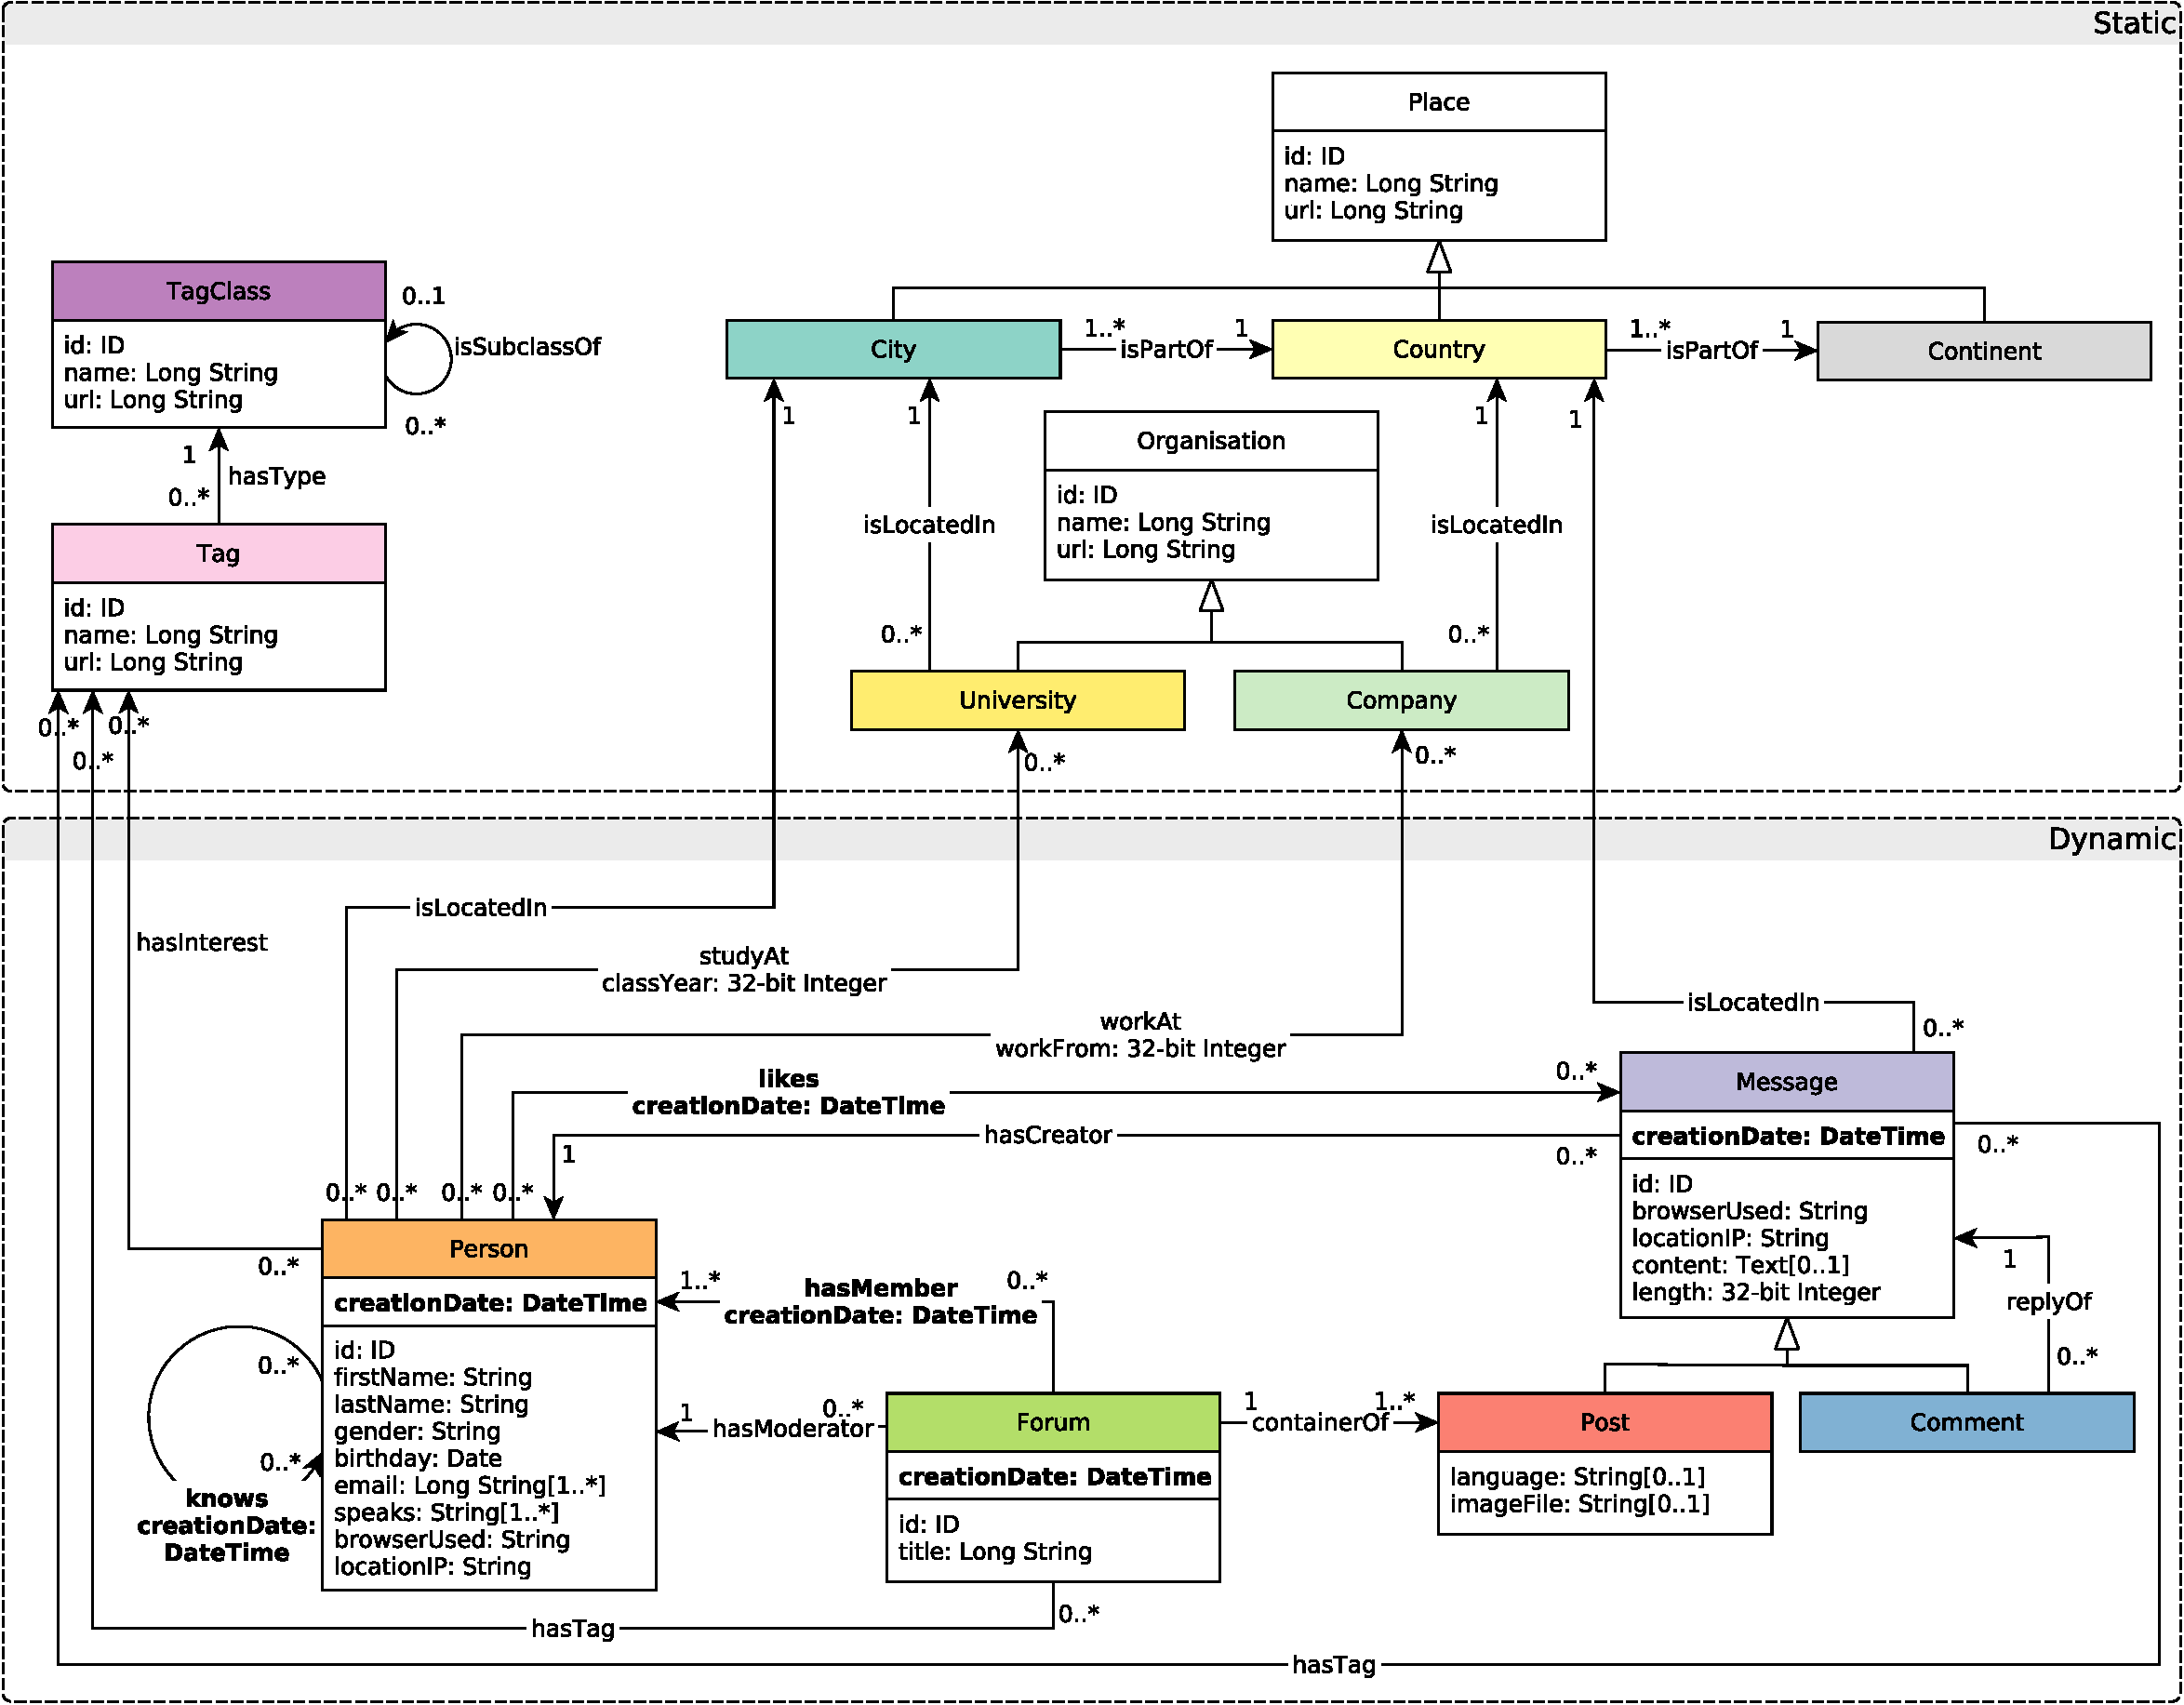
\includegraphics[width=\linewidth]{figures/schema-comfortable}
	\caption{The \ldbcsnb data schema}
	\label{figure:schema}
\end{figure}

The schema specifies different entities, their attributes and their relations.
All of them are described in the following sections.

{\flushleft \textbf{Textual Restrictions and Notes}}
\begin{itemize}
    \item Posts have content or imageFile. They have one of them but not both. The one they do not have is an empty string.
    \item Posts in a forum can be created by a non-member person if and only if that person is a modeartor.
\end{itemize}

\subsubsection{Entities}

{\flushleft \textbf{City:}} a sub-class of a Place, and represents a
city of the real world. City entities are used to specify where persons live,
as well as where universities operate.

{\flushleft \textbf{Comment:}} a sub-class of a Message, and represents a
comment made by a person to an existing message (either a Post or a Comment).

{\flushleft \textbf{Company:}} a sub-class of an Organisation, and represents a company where persons work.


{\flushleft \textbf{Country:}} a sub-class of a Place, and represents a continent of the real world.


{\flushleft \textbf{Forum:}} a meeting point where people
post messages. Forums are characterized by the topics (represented as tags)
people in the forum are talking about. Although from the schema's perspective
it is not evident, there exist three different types of
forums: persons' personal walls, image albums, and groups. They are
distinguished by their titles. \autoref{table:forum} shows the attributes
of Forum entity.

\begin{table}[H]
    \begin{tabular}{|>{\varNameCell}p{\attributeColumnWidth}|>{\typeCell}p{\typeColumnWidth}|p{\descriptionColumnWidth}|}
        \hline
        \tableHeaderFirst{Attribute} & \tableHeader{Type} & \tableHeader{Description} \\
        \hline
        id & ID  & The identifier of the forum.\\
        \hline
        title & Long String  & The title of the forum.\\
        \hline
        creationDate & DateTime  & The date the forum was created.\\
        \hline
    \end{tabular}
    \caption{Attributes of Forum entity.}
    \label{table:forum}
\end{table}

{\flushleft \textbf{Message:}} an abstract entity that represents a message
created by a person. \autoref{table:message} shows the attributes of Message
abstract entity.

\begin{table}[H]
    \begin{tabular}{|>{\varNameCell}p{\attributeColumnWidth}|>{\typeCell}p{\typeColumnWidth}|p{\descriptionColumnWidth}|}
        \hline
        \tableHeaderFirst{Attribute} & \tableHeader{Type} & \tableHeader{Description} \\
        \hline
        id & ID  & The identifier of the message.\\
        \hline
        browserUsed & String  & The browser used by the Person to create the message.\\
        \hline
        creationDate & DateTime  & The date the message was created.\\
        \hline
        locationIP & String  & The IP of the location from which the message was created.\\
        \hline
        content & Text[0..1]  & The content of the message.\\
        \hline
        length & 32-bit Integer  & The length of the content.\\
        \hline
    \end{tabular}
    \caption{Attributes of Message interface.}
    \label{table:message}
\end{table}

{\flushleft \textbf{Organisation:}} an institution of the real
world. \autoref{table:organisation} shows the attributes of Organisation
entity.

\begin{table}[H]
    \begin{tabular}{|>{\varNameCell}p{\attributeColumnWidth}|>{\typeCell}p{\typeColumnWidth}|p{\descriptionColumnWidth}|}
        \hline
        \tableHeaderFirst{Attribute} & \tableHeader{Type} & \tableHeader{Description} \\
        \hline
        id & ID  & The identifier of the organisation.\\
        \hline
        name & Long String  & The name of the organisation.\\
        \hline
        url & Long String  & The URL of the organisation.\\
        \hline
    \end{tabular}
    \caption{Attributes of Organisation entity.}
    \label{table:organisation}
\end{table}

{\flushleft \textbf{Person:}} the avatar a real world person creates
when he/she joins the network, and contains various information about the
person as well as network related information. \autoref{table:person} shows
the attributes of Person entity.

\begin{table}[H]
    \begin{tabular}{|>{\varNameCell}p{\attributeColumnWidth}|>{\typeCell}p{\typeColumnWidth}|p{\descriptionColumnWidth}|}
        \hline
        \tableHeaderFirst{Attribute} & \tableHeader{Type} & \tableHeader{Description} \\
        \hline
        id & ID  & The identifier of the person.\\
        \hline
        firstName & String  & The first name of the person.\\
        \hline
        lastName & String  & The last name of the person.\\
        \hline
        gender & String  & The gender of the person.\\
        \hline
        birthday & Date  & The birthday of the person.\\
        \hline
        email & Long String[1..*]  & The set of emails the person has.\\
        \hline
        speaks & String[1..*]  & The set of languages the person speaks.\\
        \hline
        browserUsed & String  & The browser used by the person when he/she registered to the social network.\\
        \hline
        locationIP & String  & The IP of the location from which the person was registered to the social network.\\
        \hline
        creationDate & DateTime  & The date the person joined the social network.\\
        \hline
    \end{tabular}
    \caption{Attributes of Person entity.}
    \label{table:person}
\end{table}


{\flushleft \textbf{Place:}} a place in the world.
\autoref{table:place} shows the attributes of Place entity.

\begin{table}[H]
    \begin{tabular}{|>{\varNameCell}p{\attributeColumnWidth}|>{\typeCell}p{\typeColumnWidth}|p{\descriptionColumnWidth}|}
        \hline
        \tableHeaderFirst{Attribute} & \tableHeader{Type} & \tableHeader{Description} \\
        \hline
        id & ID  & The identifier of the place.\\
        \hline
        name & Long String  & The name of the place.\\
        \hline
        url & Long String  & The URL of the place.\\
        \hline
    \end{tabular}
    \caption{Attributes of Place entity.}
    \label{table:place}
\end{table}

{\flushleft \textbf{Post:}} a sub-class of Message, that is posted in a
forum. Posts are created by persons into the forums where they belong.
Posts contain either content or imageFile, always one of them but never both.
The one they do not have is an empty string.
\autoref{table:post} shows the attributes of Post entity.

\begin{table}[H]
    \begin{tabular}{|>{\varNameCell}p{\attributeColumnWidth}|>{\typeCell}p{\typeColumnWidth}|p{\descriptionColumnWidth}|}
        \hline
        \tableHeaderFirst{Attribute} & \tableHeader{Type} & \tableHeader{Description} \\
        \hline
        language & String[0..1]  & The language of the post.\\
        \hline
        imageFile & String[0..1]  & The image file of the post.\\
        \hline
    \end{tabular}
    \caption{Attributes of Post entity.}
    \label{table:post}
\end{table}

{\flushleft \textbf{Tag:}} a topic or a concept. Tags are used to
specify the topics of forums and posts, as well as the topics a person is
interested in. \autoref{table:tag} shows the attributes of Tag entity.

\begin{table}[H]
    \begin{tabular}{|>{\varNameCell}p{\attributeColumnWidth}|>{\typeCell}p{\typeColumnWidth}|p{\descriptionColumnWidth}|}
        \hline
        \tableHeaderFirst{Attribute} & \tableHeader{Type} & \tableHeader{Description} \\
        \hline
        id & ID  & The identifier of the tag.\\
        \hline
        name & Long String  &  The name of the tag.\\
        \hline
        url & Long String  &  The URL of the tag.\\
        \hline
    \end{tabular}
    \caption{Attributes of Tag entity.}
    \label{table:tag}
\end{table}

{\flushleft \textbf{TagClass:}} a class or a category used to build
a hierarchy of tags. \autoref{table:tagclass} shows the attributes of TagClass
entity.

\begin{table}[H]
    \begin{tabular}{|>{\varNameCell}p{\attributeColumnWidth}|>{\typeCell}p{\typeColumnWidth}|p{\descriptionColumnWidth}|}
        \hline
        \tableHeaderFirst{Attribute} & \tableHeader{Type} & \tableHeader{Description} \\
        \hline
        id & ID  & The identifier of the tagclass.\\
        \hline
        name & Long String  &  The name of the tagclass.\\
        \hline
        url & Long String  &  The URL of the tagclass.\\
        \hline
    \end{tabular}
    \caption{Attributes of TagClass entity.}
    \label{table:tagclass}
\end{table}

{\flushleft \textbf{University:}} a sub-class of Organisation,
and represents an institution where persons study.

\subsubsection{Relations}

Relations connect entities of different types. Entities are defined by their ''id'' attribute.

\begin{longtable}{|>{\varNameCell}p{2.5cm}|>{\typeCell}p{2.5cm}|>{\typeCell}p{2.5cm}|>{\edgeDirectionCell}c|p{6.5cm}|}
       \hline
        \tableHeaderFirst{Name} & \tableHeader{Tail} & \tableHeader{Head} & \tableHeader{Type} & \tableHeader{Description} \\
        \hline
        containerOf & Forum[1] & Post[1..*] & D & A Forum and a Post contained in it\\
        \hline
        hasCreator & Message[0..*] & Person[1] & D & A Message and its creator (Person)\\
        \hline
        hasInterest & Person[0..*] & Tag[0..*] & D & A Person and a Tag representing a topic the person is interested in\\
        \hline
        hasMember & Forum[0..*] &  Person[1..*] & D & A  Forum and a member (Person) of the forum

        \attributeTable{joinDate}{DateTime}{The Date the person joined the forum}

        \\
        \hline
        hasModerator & Forum[0..*] & Person[1] & D & A Forum and its moderator (Person) \\
        \hline
        hasTag & Message[0..*] & Tag[0..*] & D & A Message and a Tag representing the message's topic \\
        \hline
        hasTag & Forum[0..*] & Tag[0..*] & D & A Forum and a Tag representing the forum's topic \\
        \hline
        hasType & Tag[0..*] & TagClass[1] & D & A Tag and a TagClass the tag belongs to \\
        \hline
        isLocatedIn & Company[0..*] & Country[1] & D & A Company and its home Country \\
        \hline
        isLocatedIn & Message[0..*] & Country[1] & D & A Message and the Country from which it was issued \\
        \hline
        isLocatedIn & Person[0..*] & City[1] & D & A Person and their home City \\
        \hline
        isLocatedIn & University[0..*] & City[1] & D &  A University and the City where the university is \\
        \hline
        isPartOf & City[1..*] & Country[1] & D & A City and the Country it is part of \\
        \hline
        isPartOf & Country[1..*] & Continent[1] & D & A Country and the Continent it is part of \\
        \hline
        isSubclassOf & TagClass[0..*] & TagClass[0..1] & D & A TagClass and its parent TagClass \\
        \hline
        knows & Person[0..*] & Person[0..*] & U & Two Persons that know each other

        \attributeTable{creationDate}{DateTime}{The date the knows relation was established}

        \\
        \hline
        likes & Person[0..*] & Message[0..*] & D & A Person that likes a Message

		\attributeTable{creationDate}{DateTime}{The date the like was issued}

        \\
        \hline
        replyOf & Comment[0..*] & Message[1] & D & A Comment and the Message it replies \\
        \hline
        studyAt & Person[0..*] & University[0..*] & D & A Person and a University it has studied

		\attributeTable{classYear}{32-bit Integer}{The year the person graduated}

        \\
        \hline
        workAt & Person[0..*] & Company[0..*] & D & A Person and a Company it works

		\attributeTable{workFrom}{32-bit Integer}{The year the person started to work at that company}

        \\
        \hline
        \caption{Description of the data relations.}
        \label{table:relations}
\end{longtable}

\subsubsection{Domain Concepts}

A \emph{thread} consists of Messages, starting with a single Post and Comments that transitively reply to that Post.

\subsection{Data Generation}
\label{section:data_generation}

\ldbcsnb provides \datagen (Data Generator), which produces synthetic
datasets following the schema described above. Data
produced mimics a social network's activity during a period of time. Three
parameters determine the generated data: the number of persons, the number of
years simulated, and the starting year of simulation. \datagen is defined by the
following characteristics:

\begin{itemize}
    \item \textbf{Realism.} Data generated by \datagen mimics the
        characteristics of those found in a real social network. In \datagen,
        output attributes, cardinalities, correlations and distributions have
        been finely tuned to reproduce a real social network in each of its
        aspects On the one hand, it is aware of the  data and link distributions
        found in a real social network such as Facebook. On the other hand, it
        uses real data from DBpedia, such as property dictionaries, which are
        used to ensure that attribute values are realistic and correlated.
    \item \textbf{Scalability.} Since \ldbcsnb targets systems of different
        scales and budgets, \datagen is capable of generating datasets of
        different sizes, from a few Gigabytes to Terabytes. \datagen is
        implemented following the MapReduce parallel paradigm, allowing the
        generation of small datasets in single node machines, as well as large
        datasets on commodity clusters.
    \item \textbf{Determinism.} \datagen is deterministic regardless of the number
        of cores/machines used to produce the data. This important feature
        guarantees that all Test Sponsors will face the same dataset,
        thus, making the comparisons between different systems fair and the
        benchmarks' results reproducible.
    \item \textbf{Usability.} \ldbcsnb is designed to have an affordable entry
        point. As such, \datagen's design is  severely influenced by this
        philosophy, and therefore it is designed to be as easy to use as
        possible.
\end{itemize}


\subsubsection{Resource Files}

\datagen uses a set of resource files with data
extracted from DBpedia. Conceptually, \datagen generates attribute's
values following a property dictionary model that is defined by

\begin{itemize}
    \item a dictionary $D$
    \item a ranking function $R$
    \item a probability function $F$
\end{itemize}

Dictionary D is a fixed set of values. The ranking function R is a bijection
that assigns to each value in a dictionary a unique rank between 1 and |$D$|.
The probability density function $F$ specifies how the data generator chooses
values from dictionary $D$ using the rank for each term in the dictionary. The
idea to have a separate ranking and probability function is motivated by the
need of generating correlated values: in particular, the ranking function is
typically parameterized by some parameters: different parameter values result
in different rankings. For example, in the case of a dictionary of property
firstName, the popularity of first names, might depend on the gender, country
and birthday properties. Thus, the fact that the popularity of first names in
different countries and times is different, is reflected by the different ranks
produced by function $R$ over the full dictionary of names.  \datagen uses a
dictionary for each literal property, as well as ranking functions for all
literal properties. These are materialized in a set of resource files, which
are described in \autoref{table:property_dictionaries}.

\begin{table}[H]
\begin{tabular}{|p{4cm}|p{12cm}|}
    \hline
    \tableHeaderFirst{Resource Name} & \tableHeader{Description} \\
    \hline
    Browsers & Contains a list of web browsers and their probability to be used. It is used to set the browsers used by the users.\\
    \hline
    Cities by Country & Contains a list of cites and the country they belong. It is used to assign cities to users and universities.\\
    \hline
    Companies by Country & Contains the set of companies per country. It is used to set the countries where companies operate.\\
    \hline
    Countries & Contains a list of countries and their populations. It is used to obtain the amount of people generated for each country.\\
    \hline
    Emails & Contains the set of email providers. It is used to generate the email accounts of persons.\\
    \hline
    IP Zones & Contains the set of IP ranges assigned to each country. It is used to assign the IP addresses to users.\\
    \hline
    Languages by Country & Contains the set of languages spoken in each country. It is used to set the languages spoken by each user.\\
    \hline
    Name by Country & Contains the set of names and the probability to appear in each country. It is used to assign names to persons, correlated with their countries.\\
    \hline
    Popular places by Country & Contains the set of popular places per country. These are used to set where images attached to posts are taken from.\\
    \hline
    Surnames' by Country & Contains the set of surnames and the probability to appear in each country. It is used to assign surnames to persons, correlated with their countries.\\
    \hline
    Tags by Country & Contains a set of tags and their probability to appear in each country. It is used to assign the interests to persons and forums.\\
    \hline
    Tag Classes & Contains, for each tag, the classes it belongs to.\\
    \hline
    Tag Hierarchies & Contains, for each tagClass, their parent tagClass.\\
    \hline
    Tag Matrix & Contains, for each tag, the correlation probability with the other tags. It is used enrich the tags associated to messages.\\
    \hline
    Tag Text & Contains, for each tag, a text. This is used to generate the text for messages.\\
    \hline
    Universities by City & Contains the set of universities per city. It is used to set the cities where universities operate.\\
    \hline
\end{tabular}
    \caption{Resource files}
    \label{table:property_dictionaries}
\end{table}

\subsubsection{Graph Generation}

\autoref{figure:generation_process} conceptually depicts the full data
generation process. The first step loads all the dictionaries and resource
files, and initializes the \datagen parameters.  Second, it generates all the
Persons in the graph, and the minimum necessary information to operate. Part of
these information are the interests of the persons, and the number of knows
relationships of every person, which is guided by a degree distribution
function similar to that found in Facebook~\cite{facebook_anatomy}.

The next three steps are devoted to the creation of knows relationships.  An
important aspect of real social networks, is the fact that similar persons
(with similar interests and behaviors) tend to be connected. This is known as
the Homophily principle~\cite{mcpherson2001birds,DBLP:journals/socnet/BaroneC18}, and implies the presence of
a larger amount of triangles than that expected in a random network. In order
to reproduce this characteristic, \datagen generates the edges by means of
correlation dimensions.  Given a person, the probability to be connected to
another person is typically skewed with respect to some similarity between the
persons. That is, for a person $n$ and for a small set of persons that are
somehow similar to it, there is a high connectivity probability, whereas for
most other persons, this probability is quite low. This knowledge is
exploited by \datagen to reproduce correlations.

\begin{figure}[H]
    \centering
    \includegraphics[width=1\linewidth]{figures/sndg/execution.pdf}
    \caption{The \datagen generation process.}
    \label{figure:generation_process}
\end{figure}

Given a similarity function $M(x) : n \rightarrow [0, \infty]$ that gives a score to a person,
with the characteristic that two similar persons will have similar scores, we
can sort all the persons by function $M$ and compare a person $n$ against only the
$W$ neighboring persons in the sorted array. The consequence of this approach is
that similar persons are grouped together, and the larger the
distance between two persons indicates a monotonic increase in their similarity
difference. In order to choose the persons to connect, \datagen uses a geometric
probability distribution that provides a probability for picking persons to
connect, that are between 1 and $W$ positions apart in the similarity
ranking.

Similarity functions and probability distribution functions over ranked
distance drive what kind of persons will be connected with an edge, not how
many. As stated above, the number of friends of a person is determined by a
Facebook-like distribution. The edges that will be connected to a person $n$,
are selected by randomly picking the required number of edges according to the
correlated probability distributions as discussed before. In the case that
multiple correlations exist, another probability function is used to divide the
intended number of edges between the various correlation dimensions. In \datagen,
three correlated dimensions are chosen: the first one depends on where the
person studied and when, and the second correlation dimension depends on the
interests of the person, and the third one is random (to reproduce the random
noise present in real data). Thus, \datagen has a Facebook-like distributed node
degree, and a predictable (but not fixed) average split between the reasons for
creating edges.

In the next step, person's activity, in the form of forums, posts and comments
is created. \datagen reproduces the fact that people with a larger number of
friends have a higher activity, and hence post more photos and comments to a
larger number of posts. Another important characteristic of real users'
activity in social network, are time correlations.  Usually, users' posts
creation in a social network is driven by real world events.  For
instance, one may think about an important event such as the elections in a
country, or a natural disaster. Around the time these events occur, network
activity about these events' topics sees an increase in volume. \datagen
reproduces these characteristics with the simulation of what we name as
flashmob events.  Several events are generated randomly at the beginning of the
generation process, which are assigned a random tag, and are given a time and
an intensity which represents the repercussion of the event in the real world.
When persons' posts are created, some of them are classified as flashmob posts,
and their topics and dates are assigned based on the generated flashmob events.
The volume of activity around this events is modeled following a model similar
to that described in~\cite{DBLP:conf/kdd/LeskovecBKT08}. Furthermore, in order to reproduce the
more uniform every day's user activity, \datagen also generates post uniformly
distributed along all the simulated time.

Finally, in the last step the data is serialized into the output files.

\subsubsection{Implementation Details}

\datagen is implemented using the MapReduce parallel paradigm. In MapReduce, a
Map function runs on different parts of the input data, in parallel and on many
node clusters. This function processes the input data and produces for each
result a key. Reduce functions then obtain this data and Reducers run in
parallel on many cluster nodes. The produced key simply determines the Reducer
to which the results are sent. The use of the MapReduce paradigm allows the
generator to scale considerably, allowing the generation of huge datasets by
using clusters of machines.

In the case of \datagen, the overall process is divided into three MapReduce jobs.
In the first job, each mapper generates a subset of the persons of the graph. A
key is assigned to each person using one of the similarity functions described
above. Then, reducers receive the the key-value pairs sorted by the key,
generate the knows relations following the described windowing process, and
assign to each person a new key based on another similarity function, for the
next MapReduce pass.  This process can be successively repeated for additional
correlation dimension.  Finally, the last reducer generates the remaining
information such as forums, posts and comments.

\subsection{Output Data}

\datagen produces outputs three different items:
\begin{itemize}
  \item \textbf{Dataset}: The dataset to be bulk loaded by the SUT. It
    corresponds to roughly the 90\% of the total generated network.
  \item \textbf{Update Streams}: A set of update streams containing update
    queries, which are used by the driver to generate the update queries of the
    workloads. This update
    streams correspond to the remaining 10\% of the generated dataset.
  \item \textbf{Substitution Parameters}: A set of files containing the
    different parameter bindings that will be used by the driver to generate the
    read queries of the workloads.
\end{itemize}

The SUT has to take care only of the generated Dataset to be bulk loaded.
The formats currently supported by \datagen are the following:

\subsubsection{Dataset}

\begin{itemize}
  \item \textbf{CSV variants:}
    \begin{itemize}
      \item \textbf{CsvBasic:} Data output in CSV format, one file per different entity and on file
        per different relation. Also, there is a file for those attributes whose
        cardinality is larger than one, \ie \texttt{Person.email}, \texttt{Person.speaks}.
      \item \textbf{CsvMergeForeign:} Similar to the CSV format, but the 
        relations of the form 1-to-1 and 1-to-N are stored in the entity files as
        a foreign keys.
      \item \textbf{CsvComposite:} Similar to the CsvBasic format, but uses composite attributes for storing the \texttt{Person.email}, and \texttt{Person.speaks} attributes.
      \item \textbf{CsvCompositeMergeForeign:} Has the traits of both the CsvComposite and the CsvMergeForeign formats.
    \end{itemize}
  \item \textbf{Turtle:} Dataset in Turtle format for RDF systems.
\end{itemize}



\paragraph{CsvBasic}

This is a comma separated format. Each entity, relation and properties with a
cardinality larger than one, are output in a separate file. Generated files are
summarized at \autoref{table:csv_basic}.  Depending on the number of threads used
for generating the dataset, the number of files varies, since there is a file
generated per thread. The * in the file names indicates a number between 0 and
$\mathsf{NumberOfThreads}-1$.

\begin{table}[htb]
    \scriptsize
    \centering
    \begin{tabular}{|c|p{4.6cm}|p{9.8cm}|}
    	\hline
    	\tableHeaderFirst{C}    & \tableHeader{File}                      & \tableHeader{Content}                                                                   \\
    	\hline\hline
        N                       & organisation\_*.csv                     & id | type({"university", "company"}) | name | url                                       \\
        E                       & organisation\_isLocatedIn\_place\_*.csv & Organisation.id | Place.id                                                              \\
        \hline
        N                       & place\_*.csv                            & id | name | url | type({"city", "country", "continent"})                                \\
        E                       & place\_isPartOf\_place\_*.csv           & Place.id | Place.id                                                                     \\
        \hline
        N                       & tag\_*.csv                              & id | name | url                                                                         \\
        E                       & tag\_hasType\_tagclass\_*.csv           & Tag.id | TagClass.id                                                                    \\
        \hline
        N                       & tagclass\_*.csv                         & id | name | url                                                                         \\
        E                       & tagclass\_isSubclassOf\_tagclass\_*.csv & TagClass.id | TagClass.id                                                               \\
        \hline\hline
        N                       & comment\_*.csv                          & id | creationDate | locationIP | browserUsed | content | length                         \\
        E                       & comment\_hasCreator\_person\_*.csv      & Comment.id | Person.id                                                                  \\
        E                       & comment\_hasTag\_tag\_*.csv             & Comment.id | Tag.id                                                                     \\
        E                       & comment\_isLocatedIn\_place\_*.csv      & Comment.id | Place.id                                                                   \\
        E                       & comment\_replyOf\_comment\_*.csv        & Comment.id | Comment.id                                                                 \\
        E                       & comment\_replyOf\_post\_*.csv           & Comment.id | Post.id                                                                    \\
        \hline
        N                       & forum\_*.csv                            & id | title | creationDate                                                               \\
        E                       & forum\_containerOf\_post\_*.csv         & Forum.id | Post.id                                                                      \\
        E                       & forum\_hasMember\_person\_*.csv         & Forum.id | Person.id | joinDate                                                         \\
        E                       & forum\_hasModerator\_person\_*.csv      & Forum.id | Person.id                                                                    \\
        E                       & forum\_hasTag\_tag\_*.csv               & Forum.id | Tag.id                                                                       \\
        \hline
        N                       & person\_*.csv                           & id | firstName | lastName | gender | birthday | creationDate | locationIP | browserUsed \\
        A                       & person\_email\_emailaddress\_*.csv      & Person.id | email                                                                       \\
        E                       & person\_hasInterest\_tag\_*.csv         & Person.id | Tag.id                                                                      \\
        E                       & person\_isLocatedIn\_place\_*.csv       & Person.id | Place.id                                                                    \\
        E                       & person\_knows\_person\_*.csv            & Person.id | Person.id | creationDate                                                    \\
        E                       & person\_likes\_comment\_*.csv           & Person.id | Comment.id | creationDate                                                      \\
        E                       & person\_likes\_post\_*.csv              & Person.id | Post.id | creationDate                                                      \\
        A                       & person\_speaks\_language\_*.csv         & Person.id | language                                                                    \\
        E                       & person\_studyAt\_organisation\_*.csv    & Person.id | Organisation.id | classYear                                                 \\
        E                       & person\_workAt\_organisation\_*.csv     & Person.id | Organisation.id | workFrom                                                  \\
        \hline
        N                       & post\_*.csv                             & id | imageFile | creationDate | locationIP | browserUsed | language | content | length  \\
        E                       & post\_hasCreator\_person\_*.csv         & Post.id | Person.id                                                                     \\
        E                       & post\_hasTag\_tag\_*.csv                & Post.id | Tag.id                                                                        \\
        E                       & post\_isLocatedIn\_place.csv            & Post.id | Place.id                                                                      \\
        \hline
    \end{tabular}
    \caption{Files output by the CsvBasic serializer (33 in total). Notation -- C: entity category, N: Node, E: Edge, A: Attribute.}
    \label{table:csv_basic}
\end{table}



\paragraph{CsvMergeForeign}

This is a comma separated format. It is similar to CSV, but those relations
connecting two entities A and B, where an entity A has a cardinality of one, A
is output as a column of entity B. Generated files are summarized at
\autoref{table:csv_merge_foreign}. Depending on the number of threads used for generating
the dataset, the number of files varies, since there is a file generated per
thread. The * in the file names indicates a number between 0 and $\mathsf{NumberOfThreads}-1$.

\input{table-csv-merge-foreign}

\paragraph{CsvComposite}

TODO -- \autoref{table:csv_composite}.

\begin{table}[htb]
    \scriptsize
    \centering
    \begin{tabular}{|c|p{4.6cm}|p{11.4cm}|}
    	\hline
    	\tableHeaderFirst{Ent.} & \tableHeader{File}                      & \tableHeader{Content}                                                                                       \\ \hline\hline
        N                       & organisation\_*.csv                     & id | type({"university", "company"}) | name | url                                                           \\ \hline
        E                       & organisation\_isLocatedIn\_place\_*.csv & Organisation.id | Place.id                                                                                  \\ \hline
        N                       & place\_*.csv                            & id | name | url | type({"city", "country", "continent"})                                                    \\ \hline
        E                       & place\_isPartOf\_place\_*.csv           & Place.id | Place.id                                                                                         \\ \hline
        N                       & tag\_*.csv                              & id | name | url                                                                                             \\ \hline
        E                       & tag\_hasType\_tagclass\_*.csv           & Tag.id | TagClass.id                                                                                        \\ \hline
        N                       & tagclass\_*.csv                         & id | name | url                                                                                             \\ \hline
        E                       & tagclass\_isSubclassOf\_tagclass\_*.csv & TagClass.id | TagClass.id                                                                                   \\ \hline\hline
        N                       & comment\_*.csv                          & id | creationDate | locationIP | browserUsed | content | length                                             \\ \hline
        E                       & comment\_hasCreator\_person\_*.csv      & Comment.id | Person.id                                                                                      \\ \hline
        E                       & comment\_hasTag\_tag\_*.csv             & Comment.id | Tag.id                                                                                         \\ \hline
        E                       & comment\_isLocatedIn\_place\_*.csv      & Comment.id | Place.id                                                                                       \\ \hline
        E                       & comment\_replyOf\_comment\_*.csv        & Comment.id | Comment.id                                                                                     \\ \hline
        E                       & comment\_replyOf\_post\_*.csv           & Comment.id | Post.id                                                                                        \\ \hline
        N                       & forum\_*.csv                            & id | title | creationDate                                                                                   \\ \hline
        E                       & forum\_containerOf\_post\_*.csv         & Forum.id | Post.id                                                                                          \\ \hline
        E                       & forum\_hasMember\_person\_*.csv         & Forum.id | Person.id | joinDate                                                                             \\ \hline
        E                       & forum\_hasModerator\_person\_*.csv      & Forum.id | Person.id                                                                                        \\ \hline
        E                       & forum\_hasTag\_tag\_*.csv               & Forum.id | Tag.id                                                                                           \\ \hline
        N                       & person\_*.csv                           & id | firstName | lastName | gender | birthday | creationDate | locationIP | browserUsed | language | emails \\ \hline
        E                       & person\_hasInterest\_tag\_*.csv         & Person.id | Tag.id                                                                                          \\ \hline
        E                       & person\_isLocatedIn\_place\_*.csv       & Person.id | Place.id                                                                                        \\ \hline
        E                       & person\_knows\_person\_*.csv            & Person.id | Person.id | creationDate                                                                        \\ \hline
        E                       & person\_likes\_comment\_*.csv           & Person.id | Post.id | creationDate                                                                          \\ \hline
        E                       & person\_likes\_post\_*.csv              & Person.id | Post.id | creationDate                                                                          \\ \hline
        E                       & person\_studyAt\_organisation\_*.csv    & Person.id | Organisation.id | classYear                                                                     \\ \hline
        E                       & person\_workAt\_organisation\_*.csv     & Person.id | Organisation.id | workFrom                                                                      \\ \hline
        N                       & post\_*.csv                             & id | imageFile | creationDate | locationIP | browserUsed | language | content | length                      \\ \hline
        E                       & post\_hasCreator\_person\_*.csv         & Post.id | Person.id                                                                                         \\ \hline
        E                       & post\_hasTag\_tag\_*.csv                & Post.id | Tag.id                                                                                            \\ \hline
        E                       & post\_isLocatedIn\_place.csv            & Post.id | Place.id                                                                                          \\ \hline
    \end{tabular}
    \caption{Files output by the CsvComposite serializer (31 in total). Notation -- N: Node, E: Edge.}
    \label{table:csv_composite}
\end{table}


\paragraph{CsvCompositeMergeForeign}

TODO -- \autoref{table:csv_composite_merge_foreign}.

\begin{table}[htb]
    \scriptsize
    \centering
    \begin{tabularx}{\linewidth}{|>{\sffamily}c|>{\tt}l|>{\tt}X|}
        \hline
        \tableHeaderFirst{C} & \tableHeader{File}                   & \tableHeader{Content}                                                                                               \\
        \hline\hline
        N                    & organisation\_*.csv                  & id | type | name | url | place                                                                                      \\
        \hline
        N                    & place\_*.csv                         & id | name | url | type | isPartOf                                                                                    \\
        \hline
        N                    & tag\_*.csv                           & id | name | url | hasType                                                                                           \\
        \hline
        N                    & tagclass\_*.csv                      & id | name | url | isSubclassOf                                                                                      \\
        \hline\hline
        N                    & comment\_*.csv                       & id | creationDate | locationIP | browserUsed | content | length | creator | place | replyOfPost | replyOfComment    \\
        E                    & comment\_hasTag\_tag\_*.csv          & Comment.id | Tag.id                                                                                                 \\
        \hline
        N                    & forum\_*.csv                         & id | title | creationDate | moderator                                                                               \\
        E                    & forum\_hasMember\_person\_*.csv      & Forum.id | Person.id | joinDate/creationDate                                                                        \\
        E                    & forum\_hasTag\_tag\_*.csv            & Forum.id | Tag.id                                                                                                   \\
        \hline
        N                    & person\_*.csv                        & id | firstName | lastName | gender | birthday | creationDate | locationIP | browserUsed | place | language | email  \\
        E                    & person\_hasInterest\_tag\_*.csv      & Person.id | Tag.id                                                                                                  \\
        E                    & person\_knows\_person\_*.csv         & Person.id | Person.id | creationDate                                                                                \\
        E                    & person\_likes\_comment\_*.csv        & Person.id | Post.id | creationDate                                                                                  \\
        E                    & person\_likes\_post\_*.csv           & Person.id | Post.id | creationDate                                                                                  \\
        E                    & person\_studyAt\_organisation\_*.csv & Person.id | Organisation.id | classYear                                                                             \\
        E                    & person\_workAt\_organisation\_*.csv  & Person.id | Organisation.id | workFrom                                                                              \\
        \hline
        N                    & post\_*.csv                          & id | imageFile | creationDate | locationIP | browserUsed | language | content | length | creator | Forum.id | place \\
        E                    & post\_hasTag\_tag\_*.csv             & Post.id | Tag.id                                                                                                    \\
        \hline
    \end{tabularx}
    \caption{Files output by the CsvCompositeMergeForeign serializer (18 in total). The first part of the table contains the static entites, the second part contains the dynamic ones.
        Notation -- \textsf{C}: entity category, \textsf{N}: node, \textsf{E}: edge.}
    \label{table:csv_composite_merge_foreign}
\end{table}



\paragraph{Turtle}

This serializers uses the standard Turtle format\footnote{Description of
the Turtle RDF format http://www.w3.org/TR/turtle/}. It outputs
two files: \texttt{0\_ldbc\_socialnet\_static\_dbp.ttl} and \texttt{0\_ldbc\_socialnet.ttl}, containing the static and the dynamic part of the graph, respectively.

\subsection{Scale Factors}

\ldbcsnb defines a set of scale factors (SFs), targeting systems of different
sizes and budgets.  SFs are computed based on the ASCII size in Gigabytes of
the generated output files using the CSV serializer. For example, SF 1 weighs roughly 1~GB in CSV
format, SF 3 weights roughly 3~GB and so on and so forth.  The proposed SFs are
the following: 1, 3, 10, 30, 100, 300, 1000.
Additionally, two small SFs, 0.1 and 0.3 are provided to help initial validation efforts.

The Test Sponsor may select the SF
that better fits their needs, by properly configuring the \datagen,
as described in \autoref{section:data_generation}.
The size of the resulting dataset, is mainly affected by the following
configuration parameters: the number of persons and the number of years
simulated. Different SFs are computed by scaling the number of Persons in
the network, while fixing the number of years simulated.
\autoref{tab:snsize} shows the parameters used in each of the SFs.

\begin{table}[H]
\centering
\begin{tabular}{|c||r|r|r|r|r|r|r|r|r|}
	\hline
	Scale Factor  &  0.1 &  0.3 &    1 &    3 &   10 &   30 &  100 &   300 & 1000 \\ \hline
	\# of Persons & 1.5K & 3.5K &  11K &  27K &  73K & 182K & 499K & 1.25M & 3.6M \\ \hline
	 \# of Years  &    3 &    3 &    3 &    3 &    3 &    3 &    3 &     3 &    3 \\ \hline
	 Start Year   & 2010 & 2010 & 2010 & 2010 & 2010 & 2010 & 2010 &  2010 & 2010 \\ \hline
\end{tabular}
\centering
\caption{Parameters of each scale factor.}
\label{tab:snsize}
\end{table}

For example, SF 30 consists of the activity of a social network of 182K users
during a period of three years, starting from 2010.

%In \autoref{appendix:scale_factors}, we show the statistics of each of the
%proposed SFs in detail, including distributions for some of the relations.

%%%%%%%%%%%%%%%%%%%%%%%%%%%%%%%%%%%%%%%%%%%%%%%%%%%%%%%%%%%%%%%%%%%%%%%%%%%%%%
%%%%%%%%%%%%%%%%%%%%%%%%%%%%%%%%%%%%%%%%%%%%%%%%%%%%%%%%%%%%%%%%%%%%%%%%%%%%%%
%%%%%%%%%%%%%%%%%%%%%%%%%%%%%%%%%%%%%%%%%%%%%%%%%%%%%%%%%%%%%%%%%%%%%%%%%%%%%%

\section{Benchmark Workflow}
\label{section:workflow}

The workflow of the benchmark is shown in \autoref{figure:workflow}.

\begin{figure}[htbp]
	\centering
	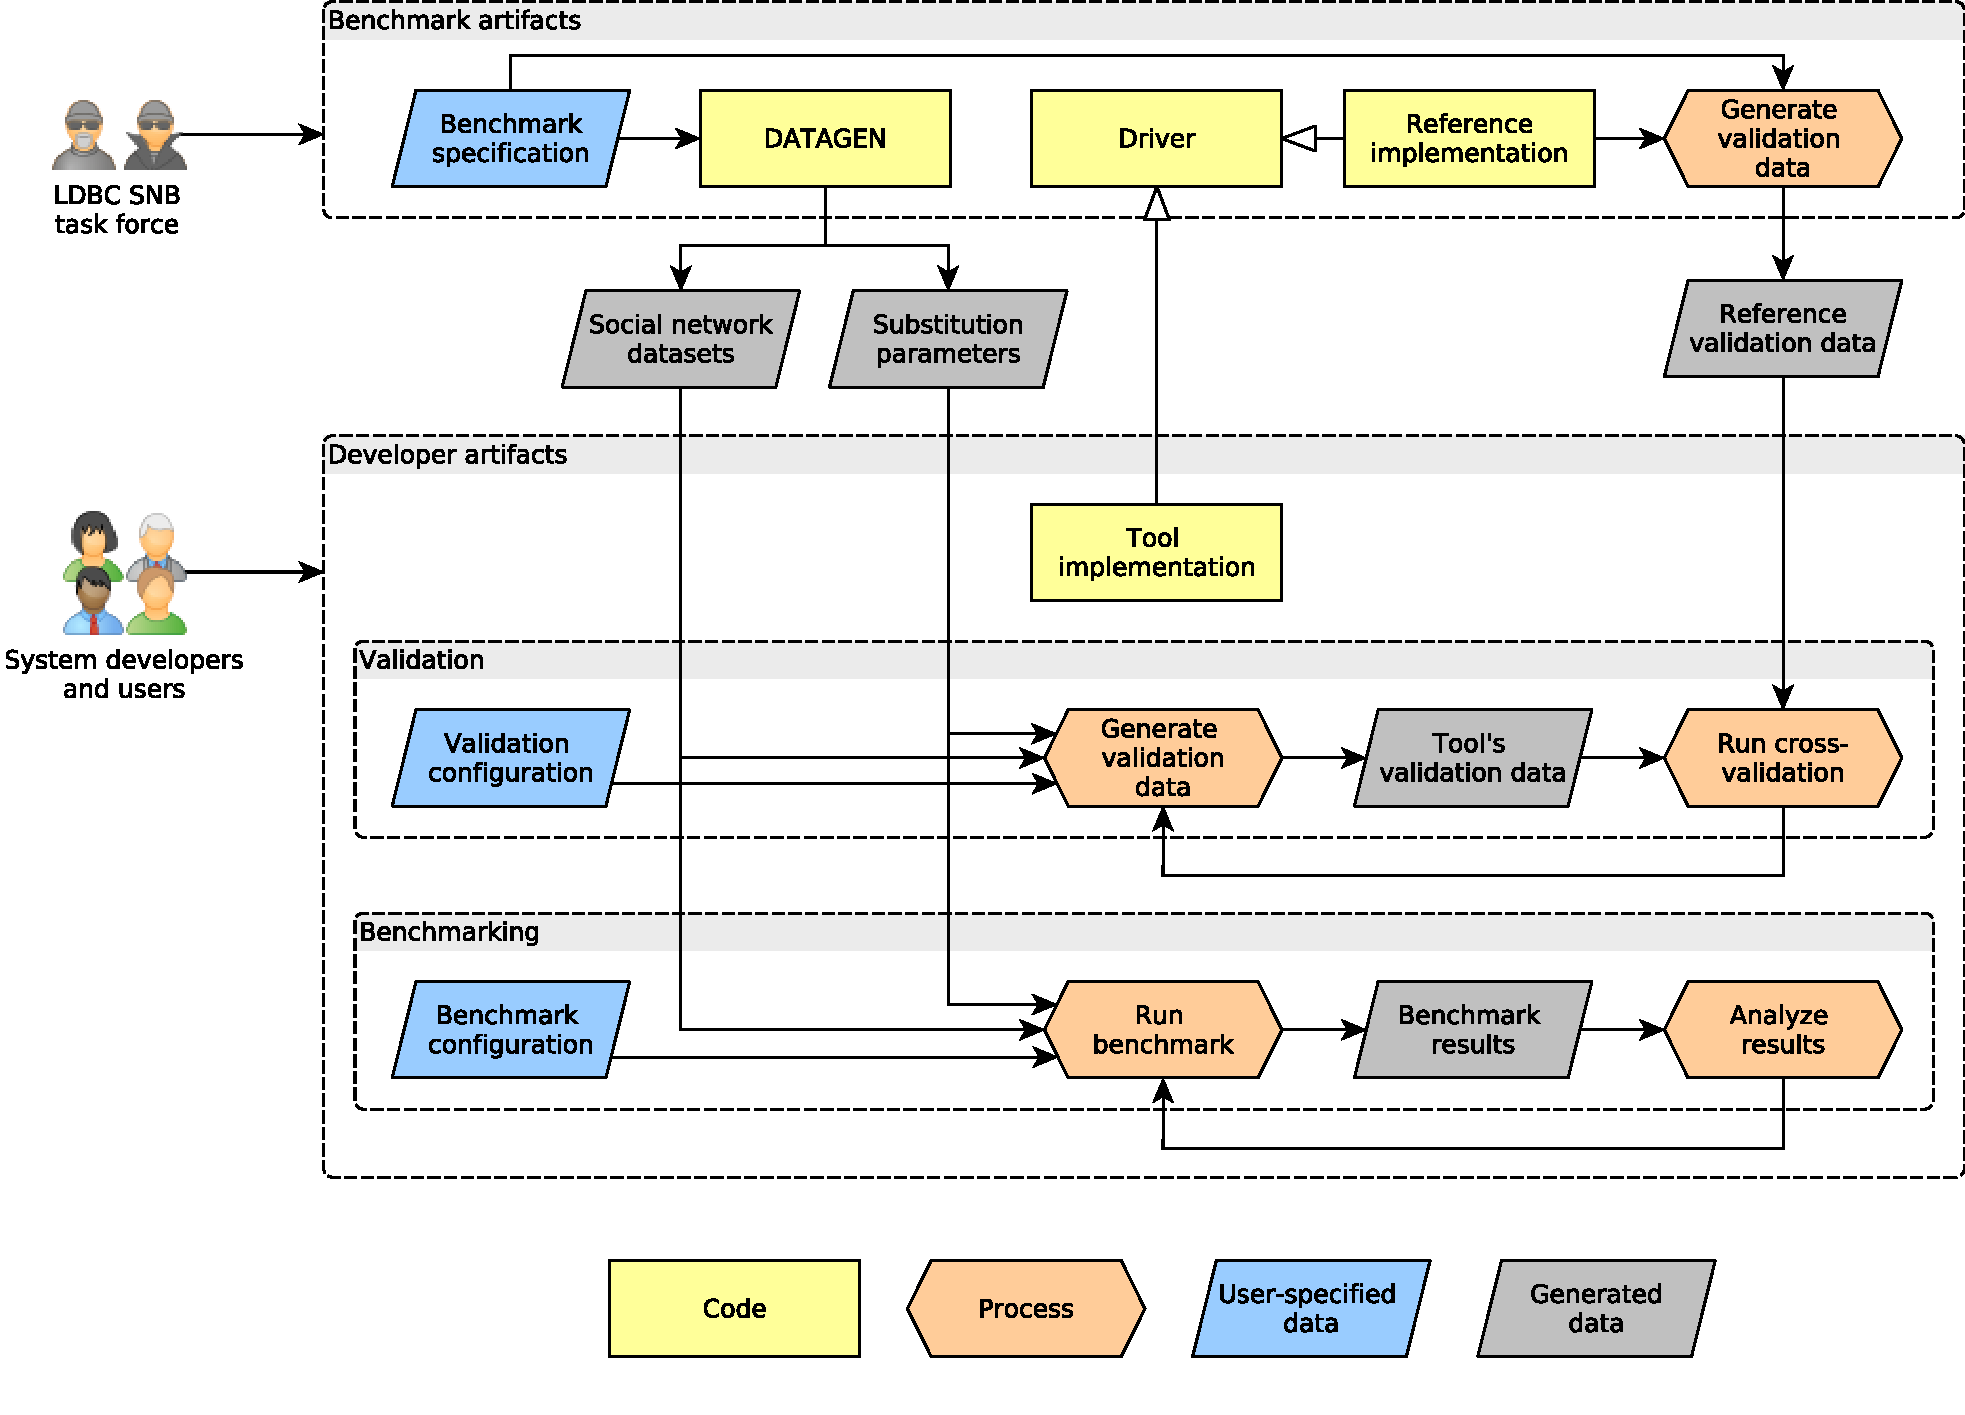
\includegraphics[width=\linewidth]{figures/workflow}
	\caption{Benchmark workflow.}
	\label{figure:workflow}
\end{figure}


\chapter{Workloads}\label{section:workloads}

\section{Query Description Format}
\label{sub:queries_structure}
Queries are described in natural language using a well-defined structure that consists of three sections:
\textit{description}, a concise textual description of the query;
\textit{parameters}, a list of input parameters and their types;
and \textit{results}, a list of expected results and their types.
The syntax used in \textit{parameters} and \textit{results} sections is as follows:

{\small
    \begin{itemize}
        \item \textbf{Entity}: entity type in the dataset.\\
            One word, possibly constructed by appending multiple words together, starting with uppercase character and following the camel case notation,
            \eg \texttt{TagClass} represents an entity of type ``TagClass''.
        \item \textbf{Relationship}: relationship type in the dataset.\\
            One word, possibly constructed by appending multiple words together, starting with lowercase character and following the camel case notation,
            and surrounded by arrow to communicate direction,
            \eg \texttt{-worksAt->} represents a directed relationship of type ``worksAt''.
        \item \textbf{Attribute}: attribute of an entity or relationship in the dataset.\\
            One word, possibly constructed by appending multiple words together, starting with lowercase character and following the camel case notation,
            and prefixed by a ``.'' to dereference the entity/relationship,
            \eg \texttt{Person.firstName} refers to ``firstName'' attribute on the ``Person'' entity,
            and \texttt{-studyAt->.classYear} refers to ``classYear'' attribute on the ``studyAt'' relationship.
        \item \textbf{Unordered Set}: an unordered collection of distinct elements.\\
            Surrounded by \{ and \} braces, with the element type between them,
            \eg \texttt{\{String\}} refers to a set of strings.
        \item \textbf{Ordered List}: an ordered collection where duplicate elements are allowed.\\
            Surrounded by [ and ] braces, with the element type between them,
            \eg \texttt{[String]} refers to a list of strings.
        \item \textbf{Ordered Tuple}: a fixed length, fixed order list of elements, where elements at each position of the tuple have predefined, possibly different, types. \\
            Surrounded by < and > braces, with the element types between them in a specific order
            \eg \texttt{<String, Boolean>} refers to a 2-tuple containing a string value in the first element and a boolean value in the second,
            and \texttt{[<String, Boolean>]} is an ordered list of those 2-tuples.
    \end{itemize}
}
\chapter{Interactive Workload}\label{section:workload}

\section{Query Specifications}

\subsection{Complex Reads Query Descriptions}

\renewcommand*{\arraystretch}{1.1}

\subsection*{Interactive / complex / 1}
\label{section:interactive-complex-read-01}

% change \emph{} to use sans-serif font
\let\oldemph\emph
\renewcommand{\emph}[1]{{\footnotesize \sf #1}}

\renewcommand{\currentQueryCard}{1}
\marginpar{
	\raggedleft
	\vspace{0.22ex}

	\queryRefCard{interactive-complex-read-01}{IC}{1}\\
	\queryRefCard{interactive-complex-read-02}{IC}{2}\\
	\queryRefCard{interactive-complex-read-03}{IC}{3}\\
	\queryRefCard{interactive-complex-read-04}{IC}{4}\\
	\queryRefCard{interactive-complex-read-05}{IC}{5}\\
	\queryRefCard{interactive-complex-read-06}{IC}{6}\\
	\queryRefCard{interactive-complex-read-07}{IC}{7}\\
	\queryRefCard{interactive-complex-read-08}{IC}{8}\\
	\queryRefCard{interactive-complex-read-09}{IC}{9}\\
	\queryRefCard{interactive-complex-read-10}{IC}{10}\\
	\queryRefCard{interactive-complex-read-11}{IC}{11}\\
	\queryRefCard{interactive-complex-read-12}{IC}{12}\\
	\queryRefCard{interactive-complex-read-13}{IC}{13}\\
	\queryRefCard{interactive-complex-read-14}{IC}{14}\\
}


\noindent\begin{tabularx}{\queryCardWidth}{|>{\queryPropertyCell}p{\queryPropertyCellWidth}|X|}
	\hline
	query & Interactive / complex / 1 \\ \hline
%
	title & Friends with certain name \\ \hline
%
	pattern & \multicolumn{1}{c|}{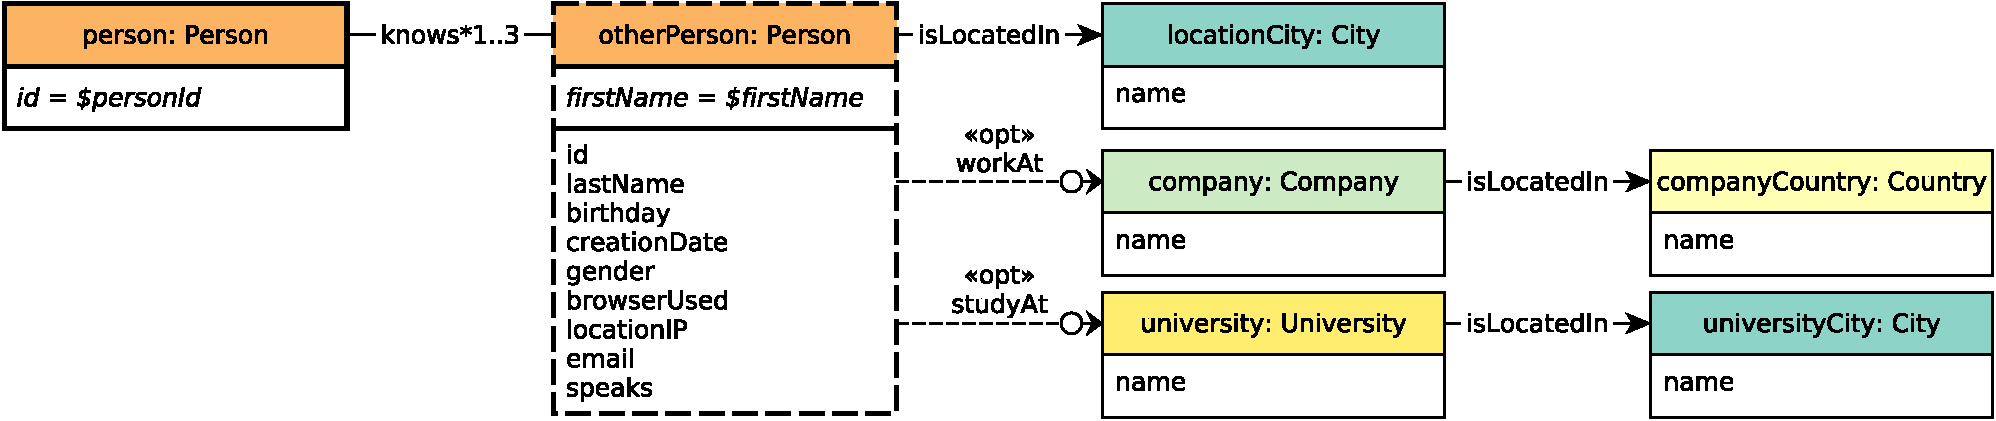
\includegraphics[scale=\patternscale,margin=0cm .2cm]{patterns/interactive-complex-read-01}} \\ \hline
%
	desc. & Given a start Person, find Persons with a given first name that the
start Person is connected to (excluding start Person) by at most 3 steps
via Knows relationships. Return Persons, including summaries of the
Persons workplaces and places of study.
 \\ \hline
%
	
		params &
		\innerCardVSpace{\begin{tabularx}{\attributeCardWidth}{|>{\paramNumberCell}c|>{\varNameCell}M|>{\typeCell}m{\typeWidth}|Y|} \hline
		$\mathsf{1}$ & Person.id
 & ID
 &  \\ \hline
		$\mathsf{2}$ & Person.firstName
 & String
 &  \\ \hline
		\end{tabularx}}\innerCardVSpace \\ \hline
	
%
	
		result &
		\innerCardVSpace{\begin{tabularx}{\attributeCardWidth}{|>{\resultNumberCell}c|>{\varNameCell}M|>{\typeCell}m{\typeWidth}|>{\resultOriginCell}c|Y|} \hline
		$\mathsf{1}$ & Person.id & ID & R &
				 \\ \hline
		$\mathsf{2}$ & Person.lastName & String & R &
				 \\ \hline
		$\mathsf{3}$ & distanceFromPerson & 32-bit Integer & R &
				1..3
 \\ \hline
		$\mathsf{4}$ & Person.birthday & Date & R &
				 \\ \hline
		$\mathsf{5}$ & Person.creationDate & DateTime & R &
				 \\ \hline
		$\mathsf{6}$ & Person.gender & String & R &
				 \\ \hline
		$\mathsf{7}$ & Person.browserUsed & String & R &
				 \\ \hline
		$\mathsf{8}$ & Person.locationIP & String & R &
				 \\ \hline
		$\mathsf{9}$ & \{Person.email\} & \{String\} & R &
				 \\ \hline
		$\mathsf{10}$ & \{Person.speaks\} & \{String\} & R &
				 \\ \hline
		$\mathsf{11}$ & Person-isLocatedIn-\textgreater{}Place.name & String & R &
				 \\ \hline
		$\mathsf{12}$ & \{Person-studyAt-\textgreater{}University.name,
Person-studyAt-\textgreater{}.classYear,
Person-studyAt-\textgreater{}University-isLocatedIn-\textgreater{}City.name\} & \{\textless{}String, 32-bit Integer, String\textgreater{}\} & R &
				 \\ \hline
		$\mathsf{13}$ & \{Person-workAt-\textgreater{}Company.name,
Person-workAt-\textgreater{}.workFrom,
Person-workAt-\textgreater{}Company-isLocatedIn-\textgreater{}Country.name\} & \{\textless{}String, 32-bit Integer, String\textgreater{}\} & R &
				 \\ \hline
		\end{tabularx}}\innerCardVSpace \\ \hline
	
%
	
		sort		&
		\innerCardVSpace{\begin{tabularx}{\attributeCardWidth}{|>{\sortNumberCell}c|>{\varNameCell}M|>{\directionCell}c|Y|} \hline
		$\mathsf{1}$ & distanceFromPerson
 & $\asc
$ &  \\ \hline
		$\mathsf{2}$ & Person.lastName
 & $\asc
$ &  \\ \hline
		$\mathsf{3}$ & Person.id
 & $\asc
$ &  \\ \hline
		\end{tabularx}}\innerCardVSpace \\ \hline
	%
	limit & 20 \\ \hline
	%
	CPs &
	\multicolumn{1}{>{\raggedright}l|}{
		\chokePoint{2.1}, 
		\chokePoint{5.3}
		} \\ \hline
	%
	relevance &
		\footnotesize This query is a representative of a simple navigational query. It looks for paths of length 1..3 through
the knows relation, starting from a given Person and ending at a Person with a given first name. It is interesting for several
aspects. (1) It requires for a complex aggregation for returning the concatenation of universities, companies,
languages and email information of the person. (2) It tests the ability of the optimizer to move the evaluation of
sub-queries functionally dependant on the Person, after the evaluation of the top-k. (3) Its performance is
highly sensitive to properly estimating the cardinalities in each transitive path, and paying attention not to explore
already visited Persons.
 \\ \hline%
\end{tabularx}
\queryCardVSpace

% change \emph back to the old one
\let\emph\oldemph
\renewcommand*{\arraystretch}{1.1}

\noindent\begin{tabularx}{17cm}{|>{\small \sf}c|X|}
	\hline
	query    & Interactive / complex / 2 \\ \hline
%
	title       & Recent posts and comments by your friends \\ \hline
%
    pattern     & \hfill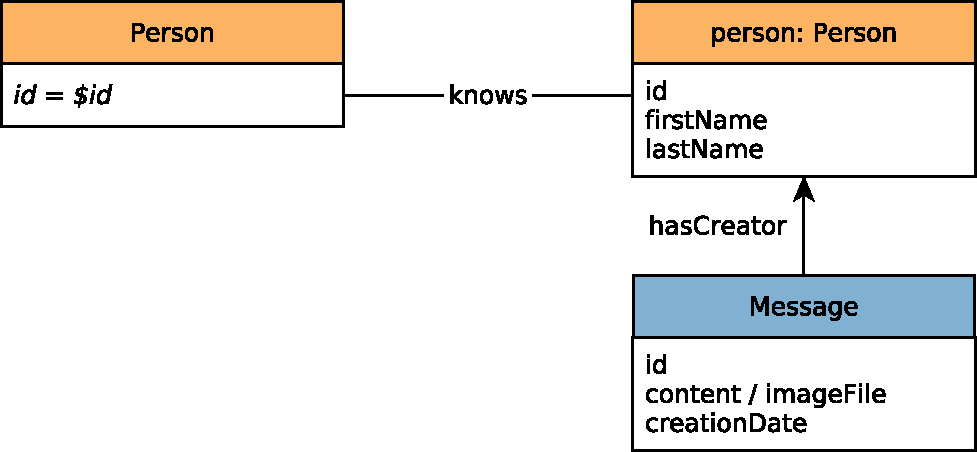
\includegraphics[scale=\patternscale,margin=0cm .2cm]{patterns/interactive-complex-read-02}\hfill\vadjust{} \\ \hline
%
	desc. & Given a start Person, find (most recent) Messages from all of that
Person's friends, that were created before (and including) a given date.
 \\ \hline
%
	
%
	params.  &
	\vspace{1.1ex}{\begin{tabularx}{14.2cm}{|c|M|m{2cm}|Y|} \hline
	\cellcolor{parameter} \color{white} $\mathsf{1}$ & \varname{Person.id} & \cellcolor{gray!20} \vartype{ID} &  \\ \hline
	\cellcolor{parameter} \color{white} $\mathsf{2}$ & \varname{date} & \cellcolor{gray!20} \vartype{DateTime} &  \\ \hline
	\end{tabularx}}\vspace{1.1ex} \\ \hline
%
	
	result      &
	\vspace{1.1ex}{\begin{tabularx}{14.2cm}{|c|M|m{2cm}|c|Y|} \hline
	\cellcolor{result} \color{white} $\mathsf{1}$ & \varname{Message-hasCreator->Person.id} & \cellcolor{gray!20} \vartype{ID} &
	    \texttt{R} &
	     \\ \hline
	\cellcolor{result} \color{white} $\mathsf{2}$ & \varname{Message-hasCreator->Person.firstName} & \cellcolor{gray!20} \vartype{String} &
	    \texttt{R} &
	     \\ \hline
	\cellcolor{result} \color{white} $\mathsf{3}$ & \varname{Message-hasCreator->Person.lastName} & \cellcolor{gray!20} \vartype{String} &
	    \texttt{R} &
	     \\ \hline
	\cellcolor{result} \color{white} $\mathsf{4}$ & \varname{Message.id} & \cellcolor{gray!20} \vartype{ID} &
	    \texttt{R} &
	     \\ \hline
	\cellcolor{result} \color{white} $\mathsf{5}$ & \varname{Message.content or Post.imageFile} & \cellcolor{gray!20} \vartype{String} &
	    \texttt{R} &
	     \\ \hline
	\cellcolor{result} \color{white} $\mathsf{6}$ & \varname{Message.creationDate} & \cellcolor{gray!20} \vartype{DateTime} &
	    \texttt{R} &
	     \\ \hline
	\end{tabularx}}\vspace{1.1ex} \\ \hline
	
%
	sort        &
	\vspace{1.1ex}{\begin{tabular}{|c|l|c|} \hline
	\cellcolor{sort} \color{white} $\mathsf{1}$ & \varname{Message.creationDate} & \cellcolor{gray!20} $\desc$ \\ \hline
	\cellcolor{sort} \color{white} $\mathsf{2}$ & \varname{Message.id} & \cellcolor{gray!20} $\asc$ \\ \hline
	\end{tabular}}\vspace{1.1ex} \\ \hline
	%
	limit       & 20 \\ \hline
	%
	CPs &
	\multicolumn{1}{>{\raggedright}l|}{
	  \chokepoint{1.1}, 
	  \chokepoint{2.2}, 
	  \chokepoint{2.3}, 
	  \chokepoint{3.2}
	  } \\ \hline
	%
    relevance &
      \small This is a navigational query looking for paths of length two, starting from a given Person, going to their friends and
from them, moving to their published Posts and Comments. This query exercices both the optimizer and how data is
stored. It tests the ability to create execution plans taking advantage of the orderings induced by some operators to
avoid performing expensive sorts. This query requires selecting Posts and Comments based on their creation date,
which might be correlated with their identifier and therefore, having intermediate results with interesting orders.
Also, messages could be stored in an order correlated with their creation date to improve data access locality. Finally,
as many of the attributes required in the projection are not needed for the execution of the query, it is expected that
the query optimizer will move the projection to the end.
 \\ \hline%
\end{tabularx}
\vspace{2ex}
\renewcommand*{\arraystretch}{1.1}

\noindent\begin{tabularx}{17cm}{|>{\small \sf}c|X|}
	\hline
	query    & Interactive / complex / 3 \\ \hline
%
	title       & Friends and friends of friends that have been to countries X and Y \\ \hline
%
    pattern     & \hfill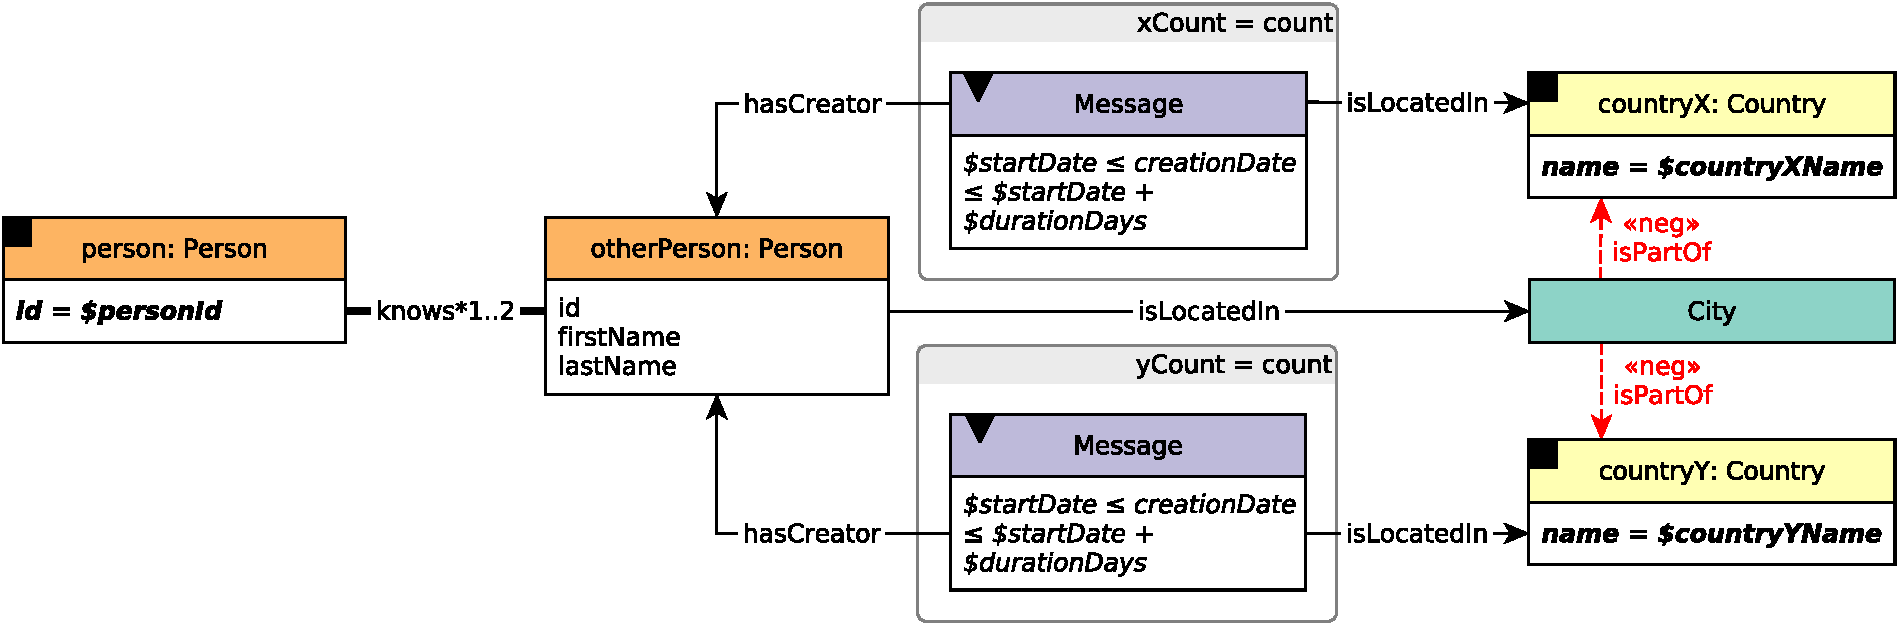
\includegraphics[scale=\patternscale,margin=0cm .2cm]{patterns/interactive-complex-read-03}\hfill\vadjust{} \\ \hline
%
	desc. & Given a start Person, find Persons that are their friends and friends of
friends (excluding start Person) that have made Posts/Comments in both
of the given Countries, X and Y, within a given period. Only Persons
that are foreign to Countries X and Y are considered, that is Persons
whose Location is not Country X or Country Y.
 \\ \hline
%
	
%
	params.  &
	\vspace{1.1ex}{\begin{tabularx}{14.66cm}{|c|M|m{2cm}|Y|} \hline
	\cellcolor{parameter} \color{white} $\mathsf{1}$ & \varname{Person.id} & \cellcolor{gray!20} \vartype{ID} &  \\ \hline
	\cellcolor{parameter} \color{white} $\mathsf{2}$ & \varname{CountryX.name} & \cellcolor{gray!20} \vartype{String} &  \\ \hline
	\cellcolor{parameter} \color{white} $\mathsf{3}$ & \varname{CountryY.name} & \cellcolor{gray!20} \vartype{String} &  \\ \hline
	\cellcolor{parameter} \color{white} $\mathsf{4}$ & \varname{startDate} & \cellcolor{gray!20} \vartype{Date} & beginning of requested period \\ \hline
	\cellcolor{parameter} \color{white} $\mathsf{5}$ & \varname{duration} & \cellcolor{gray!20} \vartype{32-bit Integer} & duration of requested period, in days the interval [startDate, startDate + Duration) is closed-open \\ \hline
	\end{tabularx}}\vspace{1.1ex} \\ \hline
%
	
	result      &
	\vspace{1.1ex}{\begin{tabularx}{14.66cm}{|c|M|m{2cm}|c|Y|} \hline
	\cellcolor{result} \color{white} $\mathsf{1}$ & \varname{Person.id} & \cellcolor{gray!20} \vartype{ID} &
	    \texttt{R} &
	     \\ \hline
	\cellcolor{result} \color{white} $\mathsf{2}$ & \varname{Person.firstName} & \cellcolor{gray!20} \vartype{String} &
	    \texttt{R} &
	     \\ \hline
	\cellcolor{result} \color{white} $\mathsf{3}$ & \varname{Person.lastName} & \cellcolor{gray!20} \vartype{String} &
	    \texttt{R} &
	     \\ \hline
	\cellcolor{result} \color{white} $\mathsf{4}$ & \varname{countX} & \cellcolor{gray!20} \vartype{32-bit Integer} &
	    \texttt{A} &
	    number of Messages from Country X made by Person within the given time \\ \hline
	\cellcolor{result} \color{white} $\mathsf{5}$ & \varname{countY} & \cellcolor{gray!20} \vartype{32-bit Integer} &
	    \texttt{A} &
	    number of Messages from Country Y made by Person within the given time \\ \hline
	\cellcolor{result} \color{white} $\mathsf{6}$ & \varname{count} & \cellcolor{gray!20} \vartype{32-bit Integer} &
	    \texttt{A} &
	    countX + countY \\ \hline
	\end{tabularx}}\vspace{1.1ex} \\ \hline
	
%
	sort        &
	\vspace{1.1ex}{\begin{tabular}{|c|l|c|} \hline
	\cellcolor{sort} \color{white} $\mathsf{1}$ & \varname{countX} & \cellcolor{gray!20} $\desc$ \\ \hline
	\cellcolor{sort} \color{white} $\mathsf{2}$ & \varname{Person.id} & \cellcolor{gray!20} $\asc$ \\ \hline
	\end{tabular}}\vspace{1.1ex} \\ \hline
	%
	limit       & 20 \\ \hline
	%
	CPs &
	\multicolumn{1}{>{\raggedright}l|}{
	  \chokepoint{2.1}, 
	  \chokepoint{3.1}, 
	  \chokepoint{5.1}
	  } \\ \hline
	%
    relevance &
      \small This query looks for paths of length two and three, starting from a Person, going to friends or friends of friends, and
then moving to Messages. This query tests the ability of the query optimizer to select the most efficient join ordering,
which will depend on the cardinalities of the intermediate results. Many friends of friends can be duplicate, then it is
expected to eliminate duplicates and those people prior to access the Post and Comments, as well as eliminate those
friends from countries X and Y, as the size of the intermediate results can be severely affected. A possible structural
optimization could be to materialize the number of Posts and Comments created by a person, and progressively
filter those people that could not even fall in the top 20 even having all their posts in the countries X and Y.
 \\ \hline%
\end{tabularx}
\vspace{2ex}
\renewcommand*{\arraystretch}{1.1}

\label{sec:interactive-complex-read-04}
\noindent\begin{tabularx}{\queryCardWidth}{|>{\queryPropertyCell}c|X|}
	\hline
	query & Interactive / complex / 4 \\ \hline
%
	title & New topics \\ \hline
%
    pattern & \hfill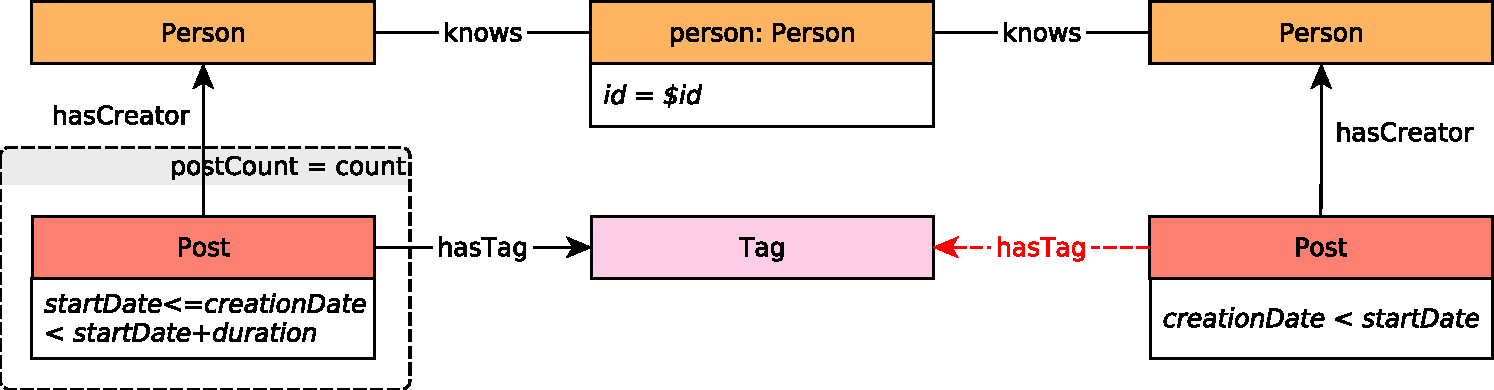
\includegraphics[scale=\patternscale,margin=0cm .2cm]{patterns/interactive-complex-read-04}\hfill\vadjust{} \\ \hline
%
	desc. & Given a start Person, find Tags that are attached to Posts that were
created by that Person's friends. Only include Tags that were attached
to friends' Posts created within a given time interval, and that were
never attached to friends' Posts created before this interval.
 \\ \hline
%
	
%
	params &
	\innerCardVSpace{\begin{tabularx}{\attributeCardWidth}{|>{\paramNumberCell}c|>{\varNameCell}M|>{\typeCell}m{\typeWidth}|Y|} \hline
	\cellcolor{parameter} \color{white} \footnotesize $\mathsf{1}$ &Person.id& ID &  \\ \hline
	\cellcolor{parameter} \color{white} \footnotesize $\mathsf{2}$ &startDate& Date &  \\ \hline
	\cellcolor{parameter} \color{white} \footnotesize $\mathsf{3}$ &duration& 32-bit Integer & duration of requested period, in days the interval [startDate, startDate + Duration) is closed-open \\ \hline
	\end{tabularx}}\innerCardVSpace \\ \hline
%
	
        result &
        \innerCardVSpace{\begin{tabularx}{\attributeCardWidth}{|>{\resultNumberCell}c|>{\varNameCell}M|>{\typeCell}m{\typeWidth}|>{\resultOriginCell}c|Y|} \hline
        $\mathsf{1}$ & Tag.name & String &R&
                 \\ \hline
        $\mathsf{2}$ & count & 32-bit Integer &A&
                number of Posts made within the given time interval that have this Tag \\ \hline
        \end{tabularx}}\innerCardVSpace \\ \hline
	
%
	sort        &
        \innerCardVSpace{\begin{tabular}{|>{\sortNumberCell}c|>{\varNameCell}l|>{\directionCell}c|} \hline
        $\mathsf{1}$ & count & $\desc$ \\ \hline
        $\mathsf{2}$ & Tag.name & $\asc$ \\ \hline
        \end{tabular}}\innerCardVSpace \\ \hline
	%
	limit & 10 \\ \hline
	%
	CPs &
	\multicolumn{1}{>{\raggedright}l|}{
	    \chokePoint{2.3}
	    } \\ \hline
	%
    relevance &
        \small This query looks for paths of length two, starting from a given Person, moving to Posts and then to Tags. It tests
the ability of the query optimizer to properly select the usage of hash joins or index based joins, depending on the
cardinality of the intermediate results. These cardinalities are clearly affected by the input Person, the number of
friends, the variety of Tags, the time interval and the number of Posts.
 \\ \hline%
\end{tabularx}
\queryCardVSpace
\renewcommand*{\arraystretch}{1.1}

\subsection*{Interactive / complex / 5}
\label{section:interactive-complex-read-05}

\noindent\begin{tabularx}{\queryCardWidth}{|>{\queryPropertyCell}p{\queryPropertyCellWidth}|X|}
	\hline
	query & Interactive / complex / 5 \\ \hline
%
	title & New groups
 \\ \hline
%
	pattern & \hfill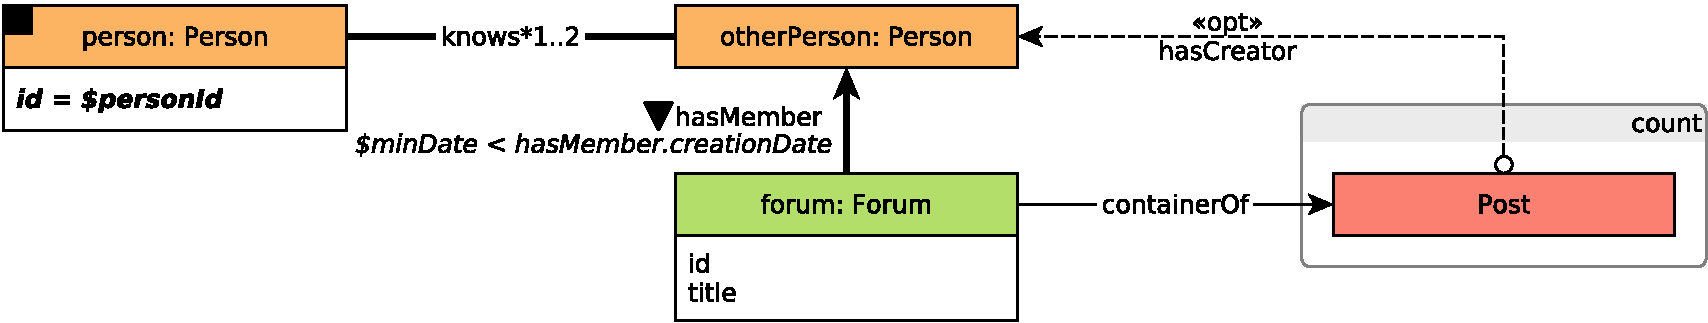
\includegraphics[scale=\patternscale,margin=0cm .2cm]{patterns/interactive-complex-read-05}\hfill\vadjust{} \\ \hline
%
	desc. & Given a start Person, find the Forums which that Person's friends and
friends of friends (excluding start Person) became Members of after a
given date. For each forum find the number of Posts that were created by
any of these Persons. For each Forum and consider only those Persons
which joined that particular Forum after the given date.
 \\ \hline
%
	
		params &
		\innerCardVSpace{\begin{tabularx}{\attributeCardWidth}{|>{\paramNumberCell}c|>{\varNameCell}M|>{\typeCell}m{\typeWidth}|Y|} \hline
		$\mathsf{1}$ & Person.id
 & ID
 &  \\ \hline
		$\mathsf{2}$ & date
 & Date
 &  \\ \hline
		\end{tabularx}}\innerCardVSpace \\ \hline
	
%
	
		result &
		\innerCardVSpace{\begin{tabularx}{\attributeCardWidth}{|>{\resultNumberCell}c|>{\varNameCell}M|>{\typeCell}m{\typeWidth}|>{\resultOriginCell}c|Y|} \hline
		$\mathsf{1}$ & Forum.title
 & String
 & R &
				 \\ \hline
		$\mathsf{2}$ & count
 & 32-bit Integer
 & R &
				Number of Posts made in Forum that were created by friends
 \\ \hline
		\end{tabularx}}\innerCardVSpace \\ \hline
	
%
	
		sort		&
		\innerCardVSpace{\begin{tabular}{|>{\sortNumberCell}c|>{\varNameCell}l|>{\directionCell}c|} \hline
		$\mathsf{1}$ & count
 & $\desc
$ \\ \hline
		$\mathsf{2}$ & Forum.id
 & $\asc
$ \\ \hline
		\end{tabular}}\innerCardVSpace \\ \hline
	%
	limit & 20 \\ \hline
	%
	CPs &
	\multicolumn{1}{>{\raggedright}l|}{
		\chokePoint{2.3}, 
		\chokePoint{3.3}
		} \\ \hline
	%
	relevance &
		\small This query looks for paths of length two and three, starting from a given Person, moving to friends and friends of
friends, and then getting the Forums they are members of. Besides testing the ability of the query optimizer to select
the proper join operator, it rewards the usage of indexes, but their accesses will be presumably scattered due to the
two/three-hop search space of the query, leading to unpredictable and scattered index accesses. Having efficient
implementations of such indexes will be highly beneficial.
 \\ \hline%
\end{tabularx}
\queryCardVSpace
\renewcommand*{\arraystretch}{1.1}

\subsection*{Interactive / complex / 6}
\label{section:interactive-complex-read-06}

% change \emph{} to use sans-serif font
\let\oldemph\emph
\renewcommand{\emph}[1]{{\footnotesize \sf #1}}

\renewcommand{\currentQueryCard}{6}
\marginpar{
	\raggedleft
	\vspace{0.22ex}

	\queryRefCard{interactive-complex-read-01}{IC}{1}\\
	\queryRefCard{interactive-complex-read-02}{IC}{2}\\
	\queryRefCard{interactive-complex-read-03}{IC}{3}\\
	\queryRefCard{interactive-complex-read-04}{IC}{4}\\
	\queryRefCard{interactive-complex-read-05}{IC}{5}\\
	\queryRefCard{interactive-complex-read-06}{IC}{6}\\
	\queryRefCard{interactive-complex-read-07}{IC}{7}\\
	\queryRefCard{interactive-complex-read-08}{IC}{8}\\
	\queryRefCard{interactive-complex-read-09}{IC}{9}\\
	\queryRefCard{interactive-complex-read-10}{IC}{10}\\
	\queryRefCard{interactive-complex-read-11}{IC}{11}\\
	\queryRefCard{interactive-complex-read-12}{IC}{12}\\
	\queryRefCard{interactive-complex-read-13}{IC}{13}\\
	\queryRefCard{interactive-complex-read-14}{IC}{14}\\
}


\noindent\begin{tabularx}{\queryCardWidth}{|>{\queryPropertyCell}p{\queryPropertyCellWidth}|X|}
	\hline
	query & Interactive / complex / 6 \\ \hline
%
	title & Tag co-occurrence \\ \hline
%
	pattern & \multicolumn{1}{c|}{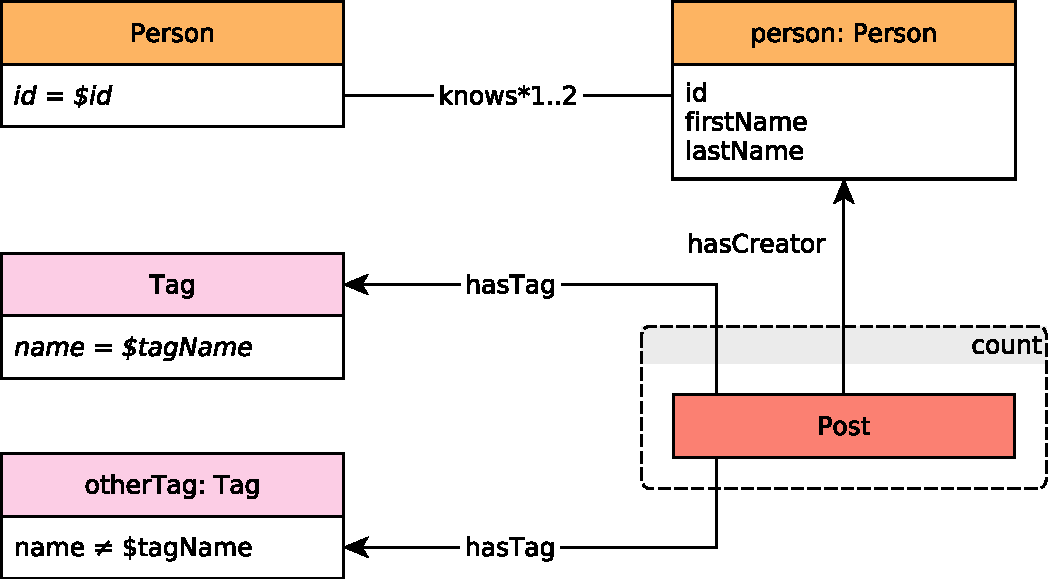
\includegraphics[scale=\patternscale,margin=0cm .2cm]{patterns/interactive-complex-read-06}} \\ \hline
%
	desc. & Given a start Person and some Tag, find the other Tags that occur
together with this Tag on Posts that were created by start Person's
friends and friends of friends (excluding start Person). Return For each
Tag, find the count of Posts that were created by these Persons, which
contain both this Tag and the given Tag.
 \\ \hline
%
	
		params &
		\innerCardVSpace{\begin{tabularx}{\attributeCardWidth}{|>{\paramNumberCell}c|>{\varNameCell}M|>{\typeCell}m{\typeWidth}|Y|} \hline
		$\mathsf{1}$ & Person.id
 & ID
 & \texttt{Person}
 \\ \hline
		$\mathsf{2}$ & Tag.name
 & String
 & \texttt{Tag}
 \\ \hline
		\end{tabularx}}\innerCardVSpace \\ \hline
	
%
	
		result &
		\innerCardVSpace{\begin{tabularx}{\attributeCardWidth}{|>{\resultNumberCell}c|>{\varNameCell}M|>{\typeCell}m{\typeWidth}|>{\resultOriginCell}c|Y|} \hline
		$\mathsf{1}$ & Tag.name & String & R &
				\texttt{tagName}
 \\ \hline
		$\mathsf{2}$ & postCount & 32-bit Integer & A &
				\texttt{postCount} -- Number of Posts that were created by friends and
friends of friends, which contain this Tag
 \\ \hline
		\end{tabularx}}\innerCardVSpace \\ \hline
	
%
	
		sort		&
		\innerCardVSpace{\begin{tabularx}{\attributeCardWidth}{|>{\sortNumberCell}c|>{\varNameCell}M|>{\directionCell}c|Y|} \hline
		$\mathsf{1}$ & postCount
 & $\desc
$ &  \\ \hline
		$\mathsf{2}$ & Tag.name
 & $\asc
$ &  \\ \hline
		\end{tabularx}}\innerCardVSpace \\ \hline
	%
	limit & 10 \\ \hline
	%
	CPs &
	\multicolumn{1}{>{\raggedright}l|}{
		\chokePoint{5.1}
		} \\ \hline
	%
	relevance &
		\footnotesize This query looks for paths of lengths three or four, starting from a Given Person, moving to friends or friends of
friends, then to Posts and finally ending at a given Tag.
 \\ \hline%
\end{tabularx}
\queryCardVSpace

% change \emph back to the old one
\let\emph\oldemph
\renewcommand*{\arraystretch}{1.1}

\subsection*{Interactive / complex / 7}
\label{section:interactive-complex-read-07}

% change \emph{} to use sans-serif font
\let\oldemph\emph
\renewcommand{\emph}[1]{{\footnotesize \sf #1}}

\renewcommand{\currentQueryCard}{7}
\input{query-cards/interactive-navbar}

\noindent\begin{tabularx}{\queryCardWidth}{|>{\queryPropertyCell}p{\queryPropertyCellWidth}|X|}
	\hline
	query & Interactive / complex / 7 \\ \hline
%
	title & Recent likers
 \\ \hline
%
	pattern & \hfill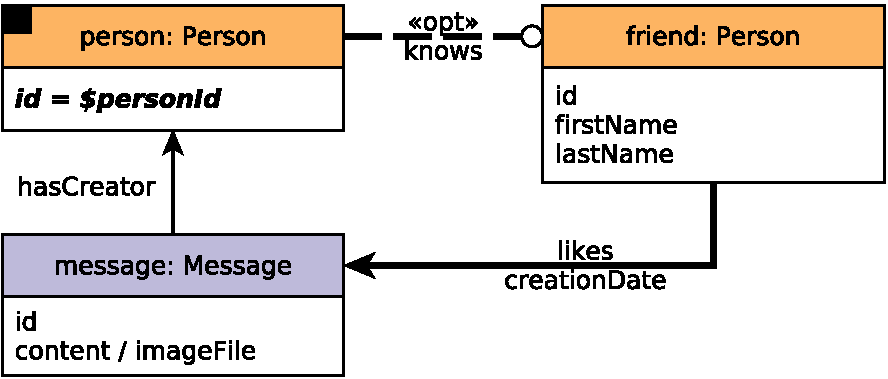
\includegraphics[scale=\patternscale,margin=0cm .2cm]{patterns/interactive-complex-read-07}\hfill\vadjust{} \\ \hline
%
	desc. & Given a start Person, find (most recent) Likes on any of start Person's
Messages. Find Persons that Liked any of start Person's Messages, the
Messages they liked most recently, creation date of that Like, and the
latency (in minutes) between creation of Messages and Like.
Additionally, for each Person found return a flag indicating whether the
liker is a friend of start Person. In the case that a Person Liked
multiple Messages at the same time, return the Message with lowest
identifier.
 \\ \hline
%
	
		params &
		\innerCardVSpace{\begin{tabularx}{\attributeCardWidth}{|>{\paramNumberCell}c|>{\varNameCell}M|>{\typeCell}m{\typeWidth}|Y|} \hline
		$\mathsf{1}$ & Person.id
 & 64-bit Integer
 &  \\ \hline
		\end{tabularx}}\innerCardVSpace \\ \hline
	
%
	
		result &
		\innerCardVSpace{\begin{tabularx}{\attributeCardWidth}{|>{\resultNumberCell}c|>{\varNameCell}M|>{\typeCell}m{\typeWidth}|>{\resultOriginCell}c|Y|} \hline
		$\mathsf{1}$ & Person.id & ID & R &
				 \\ \hline
		$\mathsf{2}$ & Person.firstName & String & R &
				 \\ \hline
		$\mathsf{3}$ & Person.lastName & String & R &
				 \\ \hline
		$\mathsf{4}$ & Like.creationDate & DateTime & R &
				 \\ \hline
		$\mathsf{5}$ & Message.id & ID & R &
				 \\ \hline
		$\mathsf{6}$ & Message.content or Post.imageFile & String & R &
				 \\ \hline
		$\mathsf{7}$ & latency & 32-bit Integer & C &
				Duration between creation of Message and Like, in minutes
 \\ \hline
		$\mathsf{8}$ & isNew & Boolean & C &
				\texttt{false} if liker Person is friend of start Person, \texttt{true}
otherwise
 \\ \hline
		\end{tabularx}}\innerCardVSpace \\ \hline
	
%
	
		sort		&
		\innerCardVSpace{\begin{tabularx}{\attributeCardWidth}{|>{\sortNumberCell}c|>{\varNameCell}M|>{\directionCell}c|Y|} \hline
		$\mathsf{1}$ & Like.creationDate
 & $\desc
$ &  \\ \hline
		$\mathsf{2}$ & Person.id
 & $\asc
$ &  \\ \hline
		\end{tabularx}}\innerCardVSpace \\ \hline
	%
	limit & 20 \\ \hline
	%
	CPs &
	\multicolumn{1}{>{\raggedright}l|}{
		\chokePoint{2.2}, 
		\chokePoint{2.3}, 
		\chokePoint{3.3}, 
		\chokePoint{5.1}
		} \\ \hline
	%
	relevance &
		\small This query looks for paths of length two, starting from a given Person, moving
to its published messages and then to Persons who liked them. It tests several aspects related to join optimization,
both at query optimization plan level and execution engine level. On the one hand, many of the columns needed for
the projection are only needed in the last stages of the query, so the optimizer is expected to delay the projection
until the end. This query implies accessing 2-hop data, and as a consequence, index accesses are expected to be
scattered. We expect to observe variate cardinalities, depending on the characteristics of the input parameter, so
properly selecting the join operators will be crucial. This query has a lot of correlated sub-queries, so it is testing
the ability to flatten the query execution plans.
 \\ \hline%
\end{tabularx}
\queryCardVSpace

% change \emph back to the old one
\renewcommand{\emph}[1]{\oldemph{#1}}
\renewcommand*{\arraystretch}{1.1}

\noindent\begin{tabularx}{17cm}{|p{1.95cm}|X|}
	\hline
	workload    & Interactive / complex \\ \hline
%
	query       & 8 \\ \hline
%
	title       & Recent replies \\ \hline
%
    pattern     & \hfill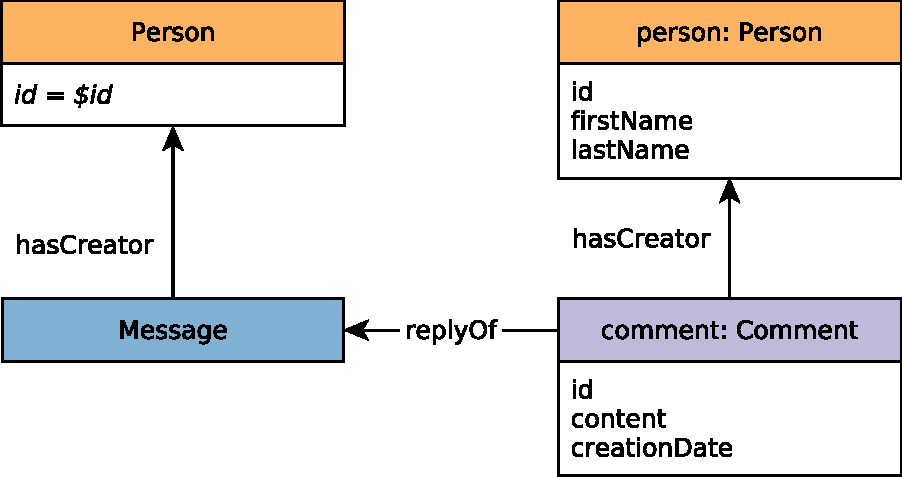
\includegraphics[scale=\patternscale,margin=0cm .2cm]{patterns/interactive-complex-read-08}\hfill\vadjust{} \\ \hline
%
	description & Given a start Person, find (most recent) Comments that are replies to
Messages of the start Person. Only consider immediate (1-hop) replies,
not the transitive (multi-hop) case. Return the reply Comments, and the
Person that created each reply Comment.
 \\ \hline
%
	
%
	parameters  &
	\vspace{1.1ex}{\begin{tabularx}{14.2cm}{|c|M|m{2cm}|Y|} \hline
	\cellcolor{parameter} \color{white} $\mathsf{1}$ & \varname{Person.id} & \cellcolor{gray!20} \vartype{ID} &  \\ \hline
	\end{tabularx}}\vspace{1.1ex} \\ \hline
%
	
	result      &
	\vspace{1.1ex}{\begin{tabularx}{14.2cm}{|c|M|m{2cm}|c|Y|} \hline
	\cellcolor{result} \color{white} $\mathsf{1}$ & \varname{Person.id} & \cellcolor{gray!20} \vartype{ID} &
	    \texttt{R} &
	     \\ \hline
	\cellcolor{result} \color{white} $\mathsf{2}$ & \varname{Person.firstName} & \cellcolor{gray!20} \vartype{String} &
	    \texttt{R} &
	     \\ \hline
	\cellcolor{result} \color{white} $\mathsf{3}$ & \varname{Person.lastName} & \cellcolor{gray!20} \vartype{String} &
	    \texttt{R} &
	     \\ \hline
	\cellcolor{result} \color{white} $\mathsf{4}$ & \varname{Comment.creationDate} & \cellcolor{gray!20} \vartype{DateTime} &
	    \texttt{R} &
	     \\ \hline
	\cellcolor{result} \color{white} $\mathsf{5}$ & \varname{Comment.id} & \cellcolor{gray!20} \vartype{ID} &
	    \texttt{R} &
	     \\ \hline
	\cellcolor{result} \color{white} $\mathsf{6}$ & \varname{Comment.content} & \cellcolor{gray!20} \vartype{String} &
	    \texttt{R} &
	     \\ \hline
	\end{tabularx}}\vspace{1.1ex} \\ \hline
	
%
	sort        &
	\vspace{1.1ex}{\begin{tabular}{|c|l|c|} \hline
	\cellcolor{sort} \color{white} $\mathsf{1}$ & \varname{Comment.creationDate} & \cellcolor{gray!20} $\desc$ \\ \hline
	\cellcolor{sort} \color{white} $\mathsf{2}$ & \varname{Comment.id} & \cellcolor{gray!20} $\asc$ \\ \hline
	\end{tabular}}\vspace{1.1ex} \\ \hline
	%
	limit       & 20 \\ \hline
	%
	%
\end{tabularx}
\vspace{2ex}
\renewcommand*{\arraystretch}{1.1}

\subsection*{Interactive / complex / 9}
\label{section:interactive-complex-read-09}

% change \emph{} to use sans-serif font
\let\oldemph\emph
\renewcommand{\emph}[1]{{\footnotesize \sf #1}}

\renewcommand{\currentQueryCard}{9}
\marginpar{
	\raggedleft
	\vspace{0.22ex}

	\queryRefCard{interactive-complex-read-01}{IC}{1}\\
	\queryRefCard{interactive-complex-read-02}{IC}{2}\\
	\queryRefCard{interactive-complex-read-03}{IC}{3}\\
	\queryRefCard{interactive-complex-read-04}{IC}{4}\\
	\queryRefCard{interactive-complex-read-05}{IC}{5}\\
	\queryRefCard{interactive-complex-read-06}{IC}{6}\\
	\queryRefCard{interactive-complex-read-07}{IC}{7}\\
	\queryRefCard{interactive-complex-read-08}{IC}{8}\\
	\queryRefCard{interactive-complex-read-09}{IC}{9}\\
	\queryRefCard{interactive-complex-read-10}{IC}{10}\\
	\queryRefCard{interactive-complex-read-11}{IC}{11}\\
	\queryRefCard{interactive-complex-read-12}{IC}{12}\\
	\queryRefCard{interactive-complex-read-13}{IC}{13}\\
	\queryRefCard{interactive-complex-read-14}{IC}{14}\\
}


\noindent\begin{tabularx}{\queryCardWidth}{|>{\queryPropertyCell}p{\queryPropertyCellWidth}|X|}
	\hline
	query & Interactive / complex / 9 \\ \hline
%
	title & Recent posts and comments by friends or friends of friends \\ \hline
%
	pattern & \multicolumn{1}{c|}{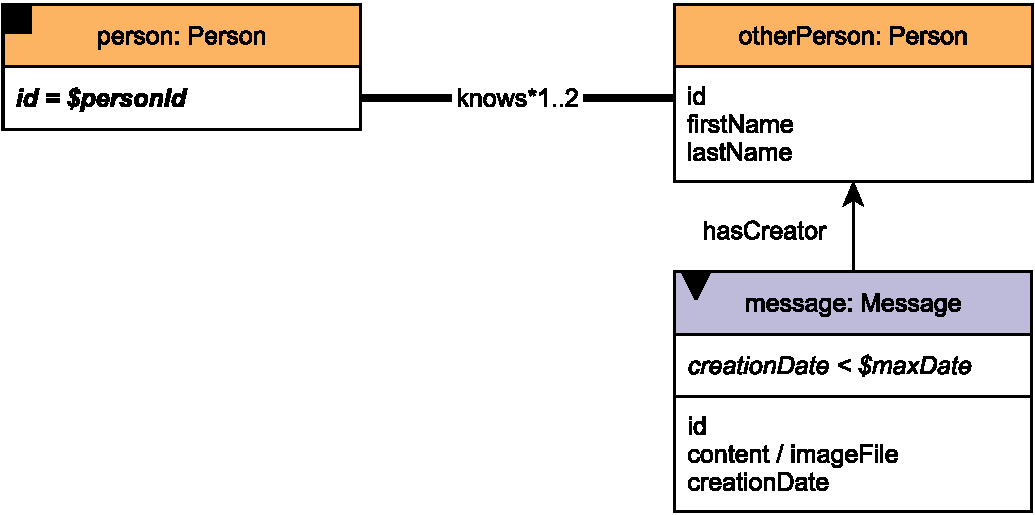
\includegraphics[scale=\patternscale,margin=0cm .2cm]{patterns/interactive-complex-read-09}} \\ \hline
%
	desc. & Given a start Person, find the (most recent) Messages created by that
Person's friends or friends of friends (excluding start Person). Only
consider the Messages created before a given date (excluding that date).
 \\ \hline
%
	
		params &
		\innerCardVSpace{\begin{tabularx}{\attributeCardWidth}{|>{\paramNumberCell}c|>{\varNameCell}M|>{\typeCell}m{\typeWidth}|Y|} \hline
		$\mathsf{1}$ & Person.id
 & ID
 &  \\ \hline
		$\mathsf{2}$ & date
 & Date
 &  \\ \hline
		\end{tabularx}}\innerCardVSpace \\ \hline
	
%
	
		result &
		\innerCardVSpace{\begin{tabularx}{\attributeCardWidth}{|>{\resultNumberCell}c|>{\varNameCell}M|>{\typeCell}m{\typeWidth}|>{\resultOriginCell}c|Y|} \hline
		$\mathsf{1}$ & Message-hasCreator-\textgreater{}Person.id & ID & R &
				\texttt{personId}
 \\ \hline
		$\mathsf{2}$ & Message-hasCreator-\textgreater{}Person.firstName & String & R &
				\texttt{personFirstName}
 \\ \hline
		$\mathsf{3}$ & Message-hasCreator-\textgreater{}Person.lastName & String & R &
				\texttt{personLastName}
 \\ \hline
		$\mathsf{4}$ & Message.id & ID & R &
				\texttt{commentOrPostId}
 \\ \hline
		$\mathsf{5}$ & Message.content or Post.imageFile & String & R &
				\texttt{commentOrPostContent}
 \\ \hline
		$\mathsf{6}$ & Message.creationDate & DateTime & R &
				\texttt{commentOrPostCreationDate}
 \\ \hline
		\end{tabularx}}\innerCardVSpace \\ \hline
	
%
	
		sort		&
		\innerCardVSpace{\begin{tabularx}{\attributeCardWidth}{|>{\sortNumberCell}c|>{\varNameCell}M|>{\directionCell}c|Y|} \hline
		$\mathsf{1}$ & Message.creationDate
 & $\desc
$ &  \\ \hline
		$\mathsf{2}$ & Message.id
 & $\asc
$ &  \\ \hline
		\end{tabularx}}\innerCardVSpace \\ \hline
	%
	limit & 20 \\ \hline
	%
	CPs &
	\multicolumn{1}{>{\raggedright}l|}{
		\chokePoint{1.1}, 
		\chokePoint{1.2}, 
		\chokePoint{2.2}, 
		\chokePoint{2.3}, 
		\chokePoint{3.2}, 
		\chokePoint{3.3}
		} \\ \hline
	%
	relevance &
		\footnotesize This query looks for paths of length two or three, starting from a given Person, moving to its friends and friends of
friends, and ending at their created Messages. This is one of the most complex queries, as the list of choke-points
indicates. This query is expected to touch variable amounts of data with entities of different characteristics, and
therefore, properly estimating cardinalities and selecting the proper operators will be crucial.
 \\ \hline%
\end{tabularx}
\queryCardVSpace

% change \emph back to the old one
\let\emph\oldemph
\renewcommand*{\arraystretch}{1.1}

\subsection*{Interactive / complex / 10}
\label{section:interactive-complex-read-10}

% change \emph{} to use sans-serif font
\let\oldemph\emph
\renewcommand{\emph}[1]{{\footnotesize \sf #1}}

\renewcommand{\currentQueryCard}{10}
\marginpar{
	\raggedleft
	\vspace{0.22ex}

	\queryRefCard{interactive-complex-read-01}{IC}{1}\\
	\queryRefCard{interactive-complex-read-02}{IC}{2}\\
	\queryRefCard{interactive-complex-read-03}{IC}{3}\\
	\queryRefCard{interactive-complex-read-04}{IC}{4}\\
	\queryRefCard{interactive-complex-read-05}{IC}{5}\\
	\queryRefCard{interactive-complex-read-06}{IC}{6}\\
	\queryRefCard{interactive-complex-read-07}{IC}{7}\\
	\queryRefCard{interactive-complex-read-08}{IC}{8}\\
	\queryRefCard{interactive-complex-read-09}{IC}{9}\\
	\queryRefCard{interactive-complex-read-10}{IC}{10}\\
	\queryRefCard{interactive-complex-read-11}{IC}{11}\\
	\queryRefCard{interactive-complex-read-12}{IC}{12}\\
	\queryRefCard{interactive-complex-read-13}{IC}{13}\\
	\queryRefCard{interactive-complex-read-14}{IC}{14}\\
}


\noindent\begin{tabularx}{\queryCardWidth}{|>{\queryPropertyCell}p{\queryPropertyCellWidth}|X|}
	\hline
	query & Interactive / complex / 10 \\ \hline
%
	title & Friend recommendation \\ \hline
%
	pattern & \multicolumn{1}{c|}{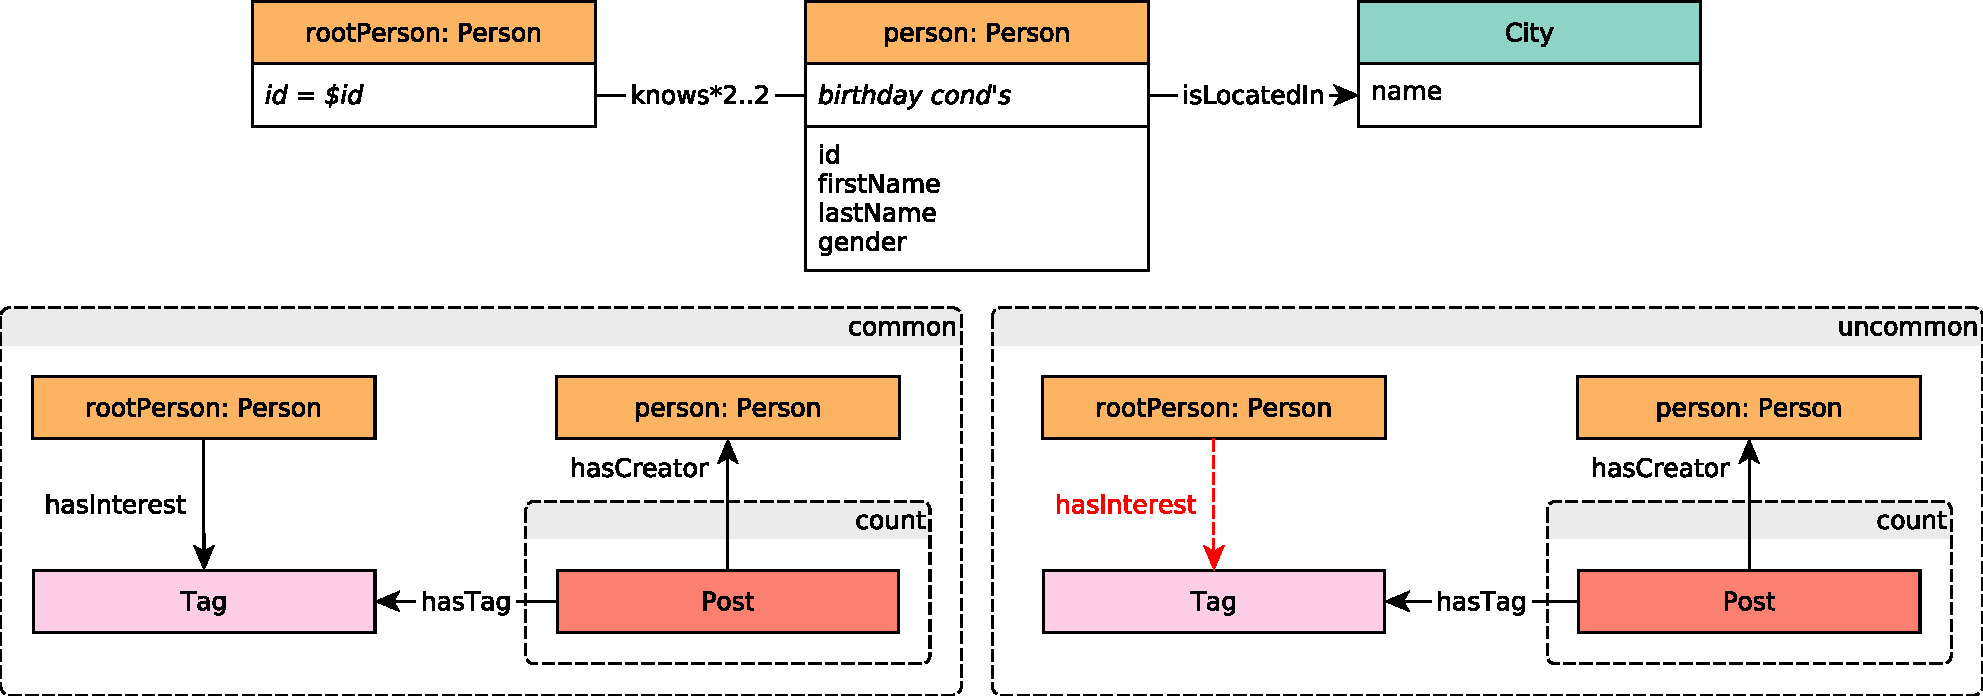
\includegraphics[scale=\patternscale,margin=0cm .2cm]{patterns/interactive-complex-read-10}} \\ \hline
%
	desc. & Given a start Person, find that Person's friends of friends (excluding
start Person, and immediate friends), who were born on or after the 21st
of a given month (in any year) and before the 22nd of the following
month. Calculate the similarity between each of these Persons and start
Person, where similarity for any Person is defined as follows:

\begin{itemize}
\tightlist
\item
  common = number of Posts created by that Person, such that the Post
  has a Tag that start Person is Interested in
\item
  uncommon = number of Posts created by that Person, such that the Post
  has no Tag that start Person is Interested in
\item
  similarity = common - uncommon
\end{itemize}
 \\ \hline
%
	
		params &
		\innerCardVSpace{\begin{tabularx}{\attributeCardWidth}{|>{\paramNumberCell}c|>{\varNameCell}M|>{\typeCell}m{\typeWidth}|Y|} \hline
		$\mathsf{1}$ & Person.id
 & ID
 &  \\ \hline
		$\mathsf{2}$ & month
 & 32-bit Integer
 & Between 1-12
 \\ \hline
		\end{tabularx}}\innerCardVSpace \\ \hline
	
%
	
		result &
		\innerCardVSpace{\begin{tabularx}{\attributeCardWidth}{|>{\resultNumberCell}c|>{\varNameCell}M|>{\typeCell}m{\typeWidth}|>{\resultOriginCell}c|Y|} \hline
		$\mathsf{1}$ & Person.id & ID & R &
				 \\ \hline
		$\mathsf{2}$ & Person.firstName & String & R &
				 \\ \hline
		$\mathsf{3}$ & Person.lastName & String & R &
				 \\ \hline
		$\mathsf{4}$ & similarity & 32-bit Integer & C &
				 \\ \hline
		$\mathsf{5}$ & Person.gender & String & R &
				 \\ \hline
		$\mathsf{6}$ & Person-isLocatedIn-\textgreater{}Place.name & String & R &
				 \\ \hline
		\end{tabularx}}\innerCardVSpace \\ \hline
	
%
	
		sort		&
		\innerCardVSpace{\begin{tabularx}{\attributeCardWidth}{|>{\sortNumberCell}c|>{\varNameCell}M|>{\directionCell}c|Y|} \hline
		$\mathsf{1}$ & similarity
 & $\desc
$ &  \\ \hline
		$\mathsf{2}$ & Person.id
 & $\asc
$ &  \\ \hline
		\end{tabularx}}\innerCardVSpace \\ \hline
	%
	limit & 10 \\ \hline
	%
	CPs &
	\multicolumn{1}{>{\raggedright}l|}{
		\chokePoint{2.3}, 
		\chokePoint{3.3}, 
		\chokePoint{4.1}, 
		\chokePoint{4.2}, 
		\chokePoint{5.1}, 
		\chokePoint{5.2}, 
		\chokePoint{6.1}, 
		\chokePoint{7.1}
		} \\ \hline
	%
	relevance &
		\footnotesize This query looks for paths of length two, starting from a Person and ending at the friends of their friends. It does
widely scattered graph traversal, and one expects no locality of in friends of friends, as these have been acquired
over a long time and have widely scattered identifiers. The join order is simple but one must see that the anti-join
for "not in my friends" is better with hash. Also the last pattern in the scalar sub-queries joining or anti-joining the
tags of the candidate's posts to interests of self should be by hash.
 \\ \hline%
\end{tabularx}
\queryCardVSpace

% change \emph back to the old one
\let\emph\oldemph
\renewcommand*{\arraystretch}{1.1}

\subsection*{Interactive / complex / 11}
\label{section:interactive-complex-read-11}

\noindent\begin{tabularx}{\queryCardWidth}{|>{\queryPropertyCell}p{\queryPropertyCellWidth}|X|}
	\hline
	query & Interactive / complex / 11 \\ \hline
%
	title & Job referral
 \\ \hline
%
	pattern & \hfill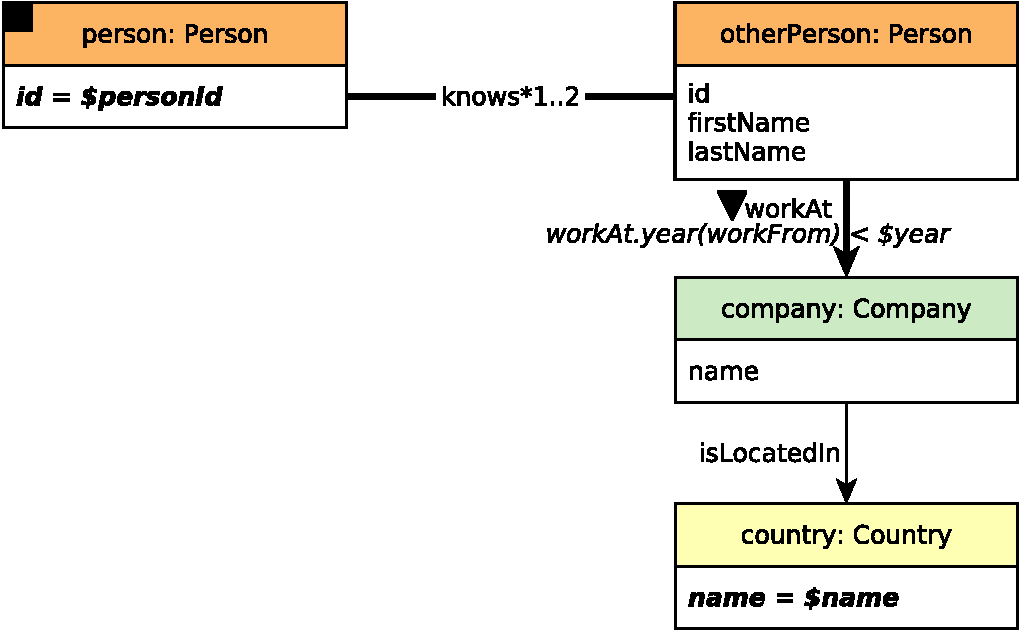
\includegraphics[scale=\patternscale,margin=0cm .2cm]{patterns/interactive-complex-read-11}\hfill\vadjust{} \\ \hline
%
	desc. & Given a start Person, find that Person's friends and friends of friends
(excluding start Person) who started Working in some Company in a given
Country, before a given date (year).
 \\ \hline
%
	
		params &
		\innerCardVSpace{\begin{tabularx}{\attributeCardWidth}{|>{\paramNumberCell}c|>{\varNameCell}M|>{\typeCell}m{\typeWidth}|Y|} \hline
		$\mathsf{1}$ & Person.id
 & ID
 &  \\ \hline
		$\mathsf{2}$ & Country.name
 & String
 &  \\ \hline
		$\mathsf{3}$ & year
 & 32-bit Integer
 &  \\ \hline
		\end{tabularx}}\innerCardVSpace \\ \hline
	
%
	
		result &
		\innerCardVSpace{\begin{tabularx}{\attributeCardWidth}{|>{\resultNumberCell}c|>{\varNameCell}M|>{\typeCell}m{\typeWidth}|>{\resultOriginCell}c|Y|} \hline
		$\mathsf{1}$ & Person.id
 & ID
 & R &
				 \\ \hline
		$\mathsf{2}$ & Person.firstName
 & String
 & R &
				 \\ \hline
		$\mathsf{3}$ & Person.lastName
 & String
 & R &
				 \\ \hline
		$\mathsf{4}$ & Person-worksAt-\textgreater{}Organisation.name
 & String
 & R &
				 \\ \hline
		$\mathsf{5}$ & Person-worksAt-\textgreater{}.worksFrom
 & 32-bit Integer
 & R &
				 \\ \hline
		\end{tabularx}}\innerCardVSpace \\ \hline
	
%
	
		sort		&
		\innerCardVSpace{\begin{tabularx}{\attributeCardWidth}{|>{\sortNumberCell}c|>{\varNameCell}M|>{\directionCell}c|Y|} \hline
		$\mathsf{1}$ & Person-worksAt-\textgreater{}.worksFrom
 & $\asc
$ &  \\ \hline
		$\mathsf{2}$ & Person.id
 & $\asc
$ &  \\ \hline
		$\mathsf{3}$ & Person-worksAt-\textgreater{}Organisation.name
 & $\desc
$ &  \\ \hline
		\end{tabularx}}\innerCardVSpace \\ \hline
	%
	limit & 10 \\ \hline
	%
	CPs &
	\multicolumn{1}{>{\raggedright}l|}{
		\chokePoint{1.4}, 
		\chokePoint{2.3}, 
		\chokePoint{2.4}, 
		\chokePoint{3.3}
		} \\ \hline
	%
	relevance &
		\small This query looks for paths of length two or three, starting from a Person, moving to friends or friends of friends,
and ending at a Company. In this query, there are selective joins and a top k order by that can be exploited for
optimizations.
 \\ \hline%
\end{tabularx}
\queryCardVSpace
\renewcommand*{\arraystretch}{1.1}

\subsection*{Interactive / complex / 12}
\label{section:interactive-complex-read-12}

% change \emph{} to use sans-serif font
\let\oldemph\emph
\renewcommand{\emph}[1]{{\footnotesize \sf #1}}

\renewcommand{\currentQueryCard}{12}
\marginpar{
	\raggedleft
	\vspace{0.22ex}

	\queryRefCard{interactive-complex-read-01}{IC}{1}\\
	\queryRefCard{interactive-complex-read-02}{IC}{2}\\
	\queryRefCard{interactive-complex-read-03}{IC}{3}\\
	\queryRefCard{interactive-complex-read-04}{IC}{4}\\
	\queryRefCard{interactive-complex-read-05}{IC}{5}\\
	\queryRefCard{interactive-complex-read-06}{IC}{6}\\
	\queryRefCard{interactive-complex-read-07}{IC}{7}\\
	\queryRefCard{interactive-complex-read-08}{IC}{8}\\
	\queryRefCard{interactive-complex-read-09}{IC}{9}\\
	\queryRefCard{interactive-complex-read-10}{IC}{10}\\
	\queryRefCard{interactive-complex-read-11}{IC}{11}\\
	\queryRefCard{interactive-complex-read-12}{IC}{12}\\
	\queryRefCard{interactive-complex-read-13}{IC}{13}\\
	\queryRefCard{interactive-complex-read-14}{IC}{14}\\
}


\noindent\begin{tabularx}{\queryCardWidth}{|>{\queryPropertyCell}p{\queryPropertyCellWidth}|X|}
	\hline
	query & Interactive / complex / 12 \\ \hline
%
	title & Expert search \\ \hline
%
	pattern & \centering 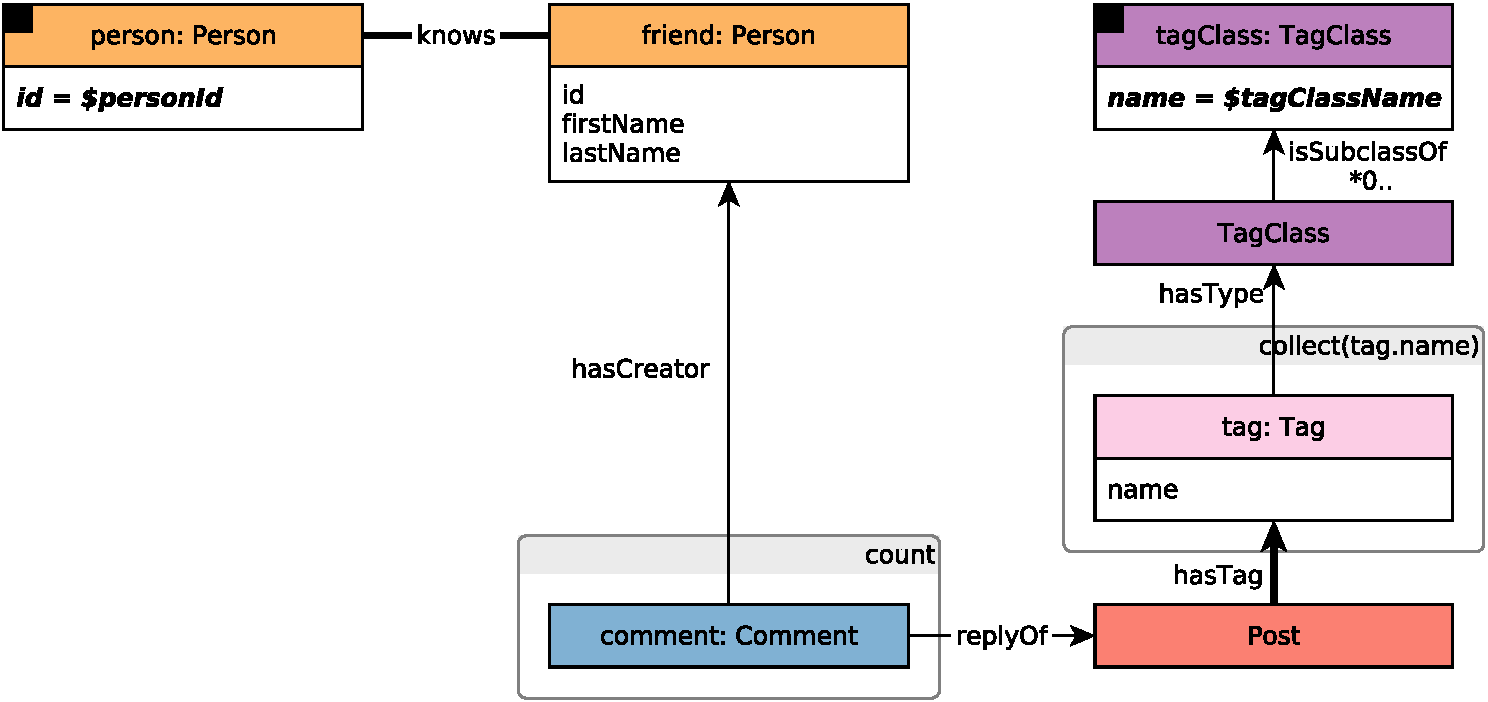
\includegraphics[scale=\patternscale,margin=0cm .2cm]{patterns/interactive-complex-read-12} \tabularnewline \hline
%
	desc. & Given a start Person, find the Comments that this Person's friends made
in reply to Posts, considering only those Comments that are immediate
(1-hop) replies to Posts, not the transitive (multi-hop) case. Only
consider Posts with a Tag in a given TagClass or in a descendent of that
TagClass. Count the number of these reply Comments, and collect the Tags
that were attached to the Posts they replied to, but only collect Tags
with the given TagClass or with a descendant of that TagClass Return
Persons with at least one reply, the reply count, and the collection of
Tags.
 \\ \hline
%
	
		params &
		\innerCardVSpace{\begin{tabularx}{\attributeCardWidth}{|>{\paramNumberCell}c|>{\varNameCell}M|>{\typeCell}m{\typeWidth}|Y|} \hline
		$\mathsf{1}$ & Person.id
 & ID
 & \texttt{personId}
 \\ \hline
		$\mathsf{2}$ & TagClass.name
 & String
 & \texttt{tagClassName}
 \\ \hline
		\end{tabularx}}\innerCardVSpace \\ \hline
	
%
	
		result &
		\innerCardVSpace{\begin{tabularx}{\attributeCardWidth}{|>{\resultNumberCell}c|>{\varNameCell}M|>{\typeCell}m{\typeWidth}|>{\resultOriginCell}c|Y|} \hline
		$\mathsf{1}$ & Person.id & ID & R &
				\texttt{personId}
 \\ \hline
		$\mathsf{2}$ & Person.firstName & String & R &
				\texttt{personFirstName}
 \\ \hline
		$\mathsf{3}$ & Person.lastName & String & R &
				\texttt{personLastName}
 \\ \hline
		$\mathsf{4}$ & \{Tag.name\} & \{String\} & R &
				\texttt{tagNames}
 \\ \hline
		$\mathsf{5}$ & replyCount & 32-bit Integer & A &
				\texttt{replyCount} -- Number of reply Comments
 \\ \hline
		\end{tabularx}}\innerCardVSpace \\ \hline
	
%
	
		sort		&
		\innerCardVSpace{\begin{tabularx}{\attributeCardWidth}{|>{\sortNumberCell}c|>{\varNameCell}M|>{\directionCell}c|Y|} \hline
		$\mathsf{1}$ & count
 & $\desc
$ &  \\ \hline
		$\mathsf{2}$ & Person.id
 & $\asc
$ &  \\ \hline
		\end{tabularx}}\innerCardVSpace \\ \hline
	%
	limit & 20 \\ \hline
	%
	CPs &
	\multicolumn{1}{>{\raggedright}l|}{
		\chokePoint{3.3}, 
		\chokePoint{7.2}, 
		\chokePoint{7.3}, 
		\chokePoint{8.2}
		} \\ \hline
	%
	relevance &
		\footnotesize This query looks for paths of length three, starting at a Person, moving to its friends, the to their Comments and
ending at the Post the Comments are replying. The chain from original post to the reply is transitive. The traversal
may be initiated at either end, the system may note that this is a tree, hence leaf to root is always best. Additionally,
a hash table can be built from either end, e.g. from the friends of self, from the tags in the category, from the or
other.
 \\ \hline%
\end{tabularx}
\queryCardVSpace

% change \emph back to the old one
\let\emph\oldemph
\renewcommand*{\arraystretch}{1.1}

\subsection*{Interactive / complex / 13}
\label{section:interactive-complex-read-13}

% change \emph{} to use sans-serif font
\let\oldemph\emph
\renewcommand{\emph}[1]{{\footnotesize \sf #1}}

\renewcommand{\currentQueryCard}{13}
\marginpar{
	\raggedleft
	\vspace{0.22ex}

	\queryRefCard{interactive-complex-read-01}{IC}{1}\\
	\queryRefCard{interactive-complex-read-02}{IC}{2}\\
	\queryRefCard{interactive-complex-read-03}{IC}{3}\\
	\queryRefCard{interactive-complex-read-04}{IC}{4}\\
	\queryRefCard{interactive-complex-read-05}{IC}{5}\\
	\queryRefCard{interactive-complex-read-06}{IC}{6}\\
	\queryRefCard{interactive-complex-read-07}{IC}{7}\\
	\queryRefCard{interactive-complex-read-08}{IC}{8}\\
	\queryRefCard{interactive-complex-read-09}{IC}{9}\\
	\queryRefCard{interactive-complex-read-10}{IC}{10}\\
	\queryRefCard{interactive-complex-read-11}{IC}{11}\\
	\queryRefCard{interactive-complex-read-12}{IC}{12}\\
	\queryRefCard{interactive-complex-read-13}{IC}{13}\\
	\queryRefCard{interactive-complex-read-14}{IC}{14}\\
}


\noindent\begin{tabularx}{\queryCardWidth}{|>{\queryPropertyCell}p{\queryPropertyCellWidth}|X|}
	\hline
	query & Interactive / complex / 13 \\ \hline
%
	title & Single shortest path \\ \hline
%
	pattern & \multicolumn{1}{c|}{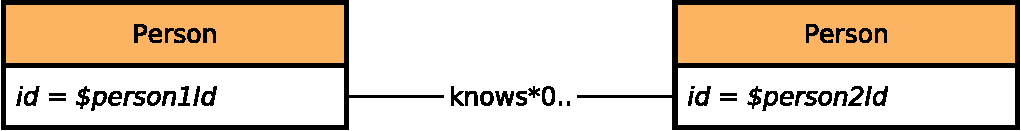
\includegraphics[scale=\patternscale,margin=0cm .2cm]{patterns/interactive-complex-read-13}} \\ \hline
%
	desc. & Given two Persons, find the shortest path between these two Persons in
the subgraph induced by the Knows relationships.

Return the length of this path:

\begin{itemize}
\tightlist
\item
  \(-1\) : no path found
\item
  \(0\): start person = end person
\item
  \(> 0\): regular case
\end{itemize}
 \\ \hline
%
	
		params &
		\innerCardVSpace{\begin{tabularx}{\attributeCardWidth}{|>{\paramNumberCell}c|>{\varNameCell}M|>{\typeCell}m{\typeWidth}|Y|} \hline
		$\mathsf{1}$ & person1.id
 & ID
 &  \\ \hline
		$\mathsf{2}$ & person2.id
 & ID
 &  \\ \hline
		\end{tabularx}}\innerCardVSpace \\ \hline
	
%
	
		result &
		\innerCardVSpace{\begin{tabularx}{\attributeCardWidth}{|>{\resultNumberCell}c|>{\varNameCell}M|>{\typeCell}m{\typeWidth}|>{\resultOriginCell}c|Y|} \hline
		$\mathsf{1}$ & length & 32-bit Integer & C &
				 \\ \hline
		\end{tabularx}}\innerCardVSpace \\ \hline
	
%
	%
	%
	CPs &
	\multicolumn{1}{>{\raggedright}l|}{
		\chokePoint{3.3}, 
		\chokePoint{7.2}, 
		\chokePoint{7.3}
		} \\ \hline
	%
	relevance &
		\small This query looks for a variable length path, starting at a given Person and finishing at an another given Person.
Proper cardinality estimation and search space prunning, will be crucial. This query also allows for possible parallel
implementations.
 \\ \hline%
\end{tabularx}
\queryCardVSpace

% change \emph back to the old one
\renewcommand{\emph}[1]{\oldemph{#1}}
\renewcommand*{\arraystretch}{1.1}

\noindent\begin{tabularx}{17cm}{|p{1.95cm}|X|}
	\hline
	workload    & Interactive / complex \\ \hline
%
	query       & 14 \\ \hline
%
	title       & Weighted/unweighted paths \\ \hline
%
    pattern     & \hfill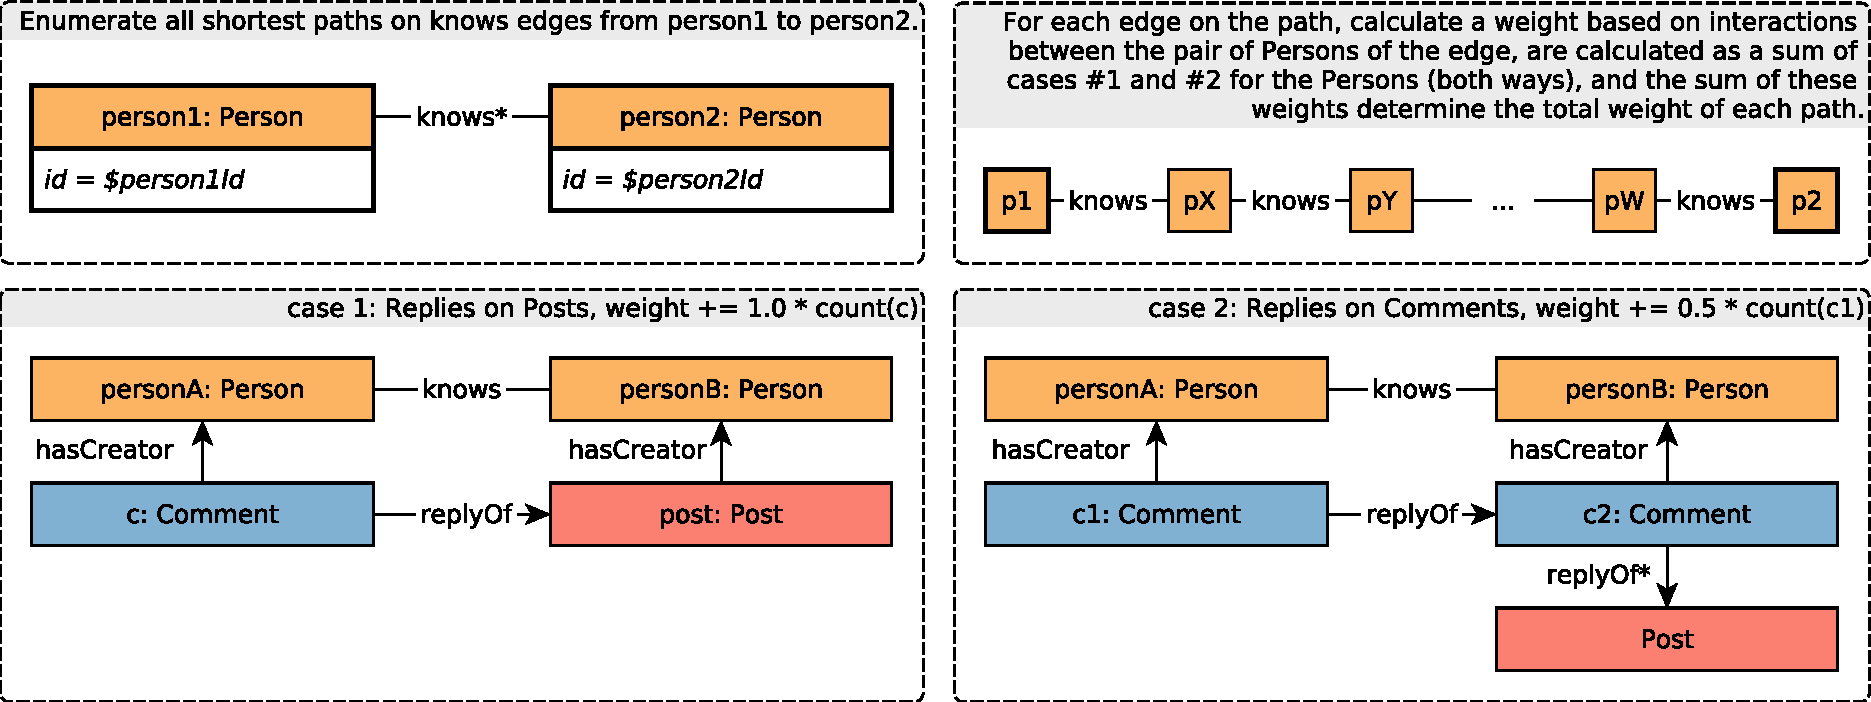
\includegraphics[scale=\patternscale,margin=0cm .2cm]{patterns/interactive-complex-read-14}\hfill\vadjust{} \\ \hline
%
	description & Given two Persons, find all (unweighted) shortest paths between these
two Persons, in the subgraph induced by the Knows relationship. Then,
for each path calculate a weight. The nodes in the path are Persons, and
the weight of a path is the sum of weights between every pair of
consecutive Person nodes in the path. The weight for a pair of Persons
is calculated such that every reply (by one of the Persons) to a Post
(by the other Person) contributes 1.0, and every reply (by ones of the
Persons) to a Comment (by the other Person) contributes 0.5. Return all
the paths with shortest length, and their weights.
 \\ \hline
%
	
%
	parameters  &
	\vspace{1.1ex}{\begin{tabularx}{14.2cm}{|c|M|m{2cm}|Y|} \hline
	\cellcolor{black!70} \color{white} $\mathsf{1}$ & \varname{person1.id} & \cellcolor{gray!20} \vartype{ID} &  \\ \hline
	\cellcolor{black!70} \color{white} $\mathsf{2}$ & \varname{person2.id} & \cellcolor{gray!20} \vartype{ID} &  \\ \hline
	\end{tabularx}}\vspace{1.1ex} \\ \hline
%
	
	result      &
	\vspace{1.1ex}{\begin{tabularx}{14.2cm}{|c|M|m{2cm}|Y|} \hline
	\cellcolor{black!70} \color{white} $\mathsf{1}$ & \varname{[Person.id]} & \cellcolor{gray!20} \vartype{[ID]} & Identifiers representing an ordered sequence of the Persons in the path \\ \hline
	\cellcolor{black!70} \color{white} $\mathsf{2}$ & \varname{weight} & \cellcolor{gray!20} \vartype{64-bit Float} &  \\ \hline
	\end{tabularx}}\vspace{1.1ex} \\ \hline
	
%
	sort        &
	\vspace{1.1ex}{\begin{tabular}{|c|l|c|} \hline
	\cellcolor{black!70} \color{white} $\mathsf{1}$ & \varname{weight} & \cellcolor{gray!20} $\desc$ \\ \hline
	\end{tabular}}\vspace{1.1ex} \\ \hline
	%
	%
	%
\end{tabularx}

\subsection{Short Reads Query Descriptions}

\todo{These could also be reworked as query cards.}
\input{query-cards/interactive-short-read-01}
\input{query-cards/interactive-short-read-02}
\input{query-cards/interactive-short-read-03}
\input{query-cards/interactive-short-read-04}
\input{query-cards/interactive-short-read-05}
\input{query-cards/interactive-short-read-06}
\input{query-cards/interactive-short-read-07}


%\renewcommand*{\arraystretch}{1.1}

\label{sec:interactive-short-read-01}
\noindent\begin{tabularx}{\queryCardWidth}{|>{\queryPropertyCell}c|X|}
	\hline
	query & Interactive / short / 1 \\ \hline
%
	title & Person Profile \\ \hline
%
    pattern & \hfill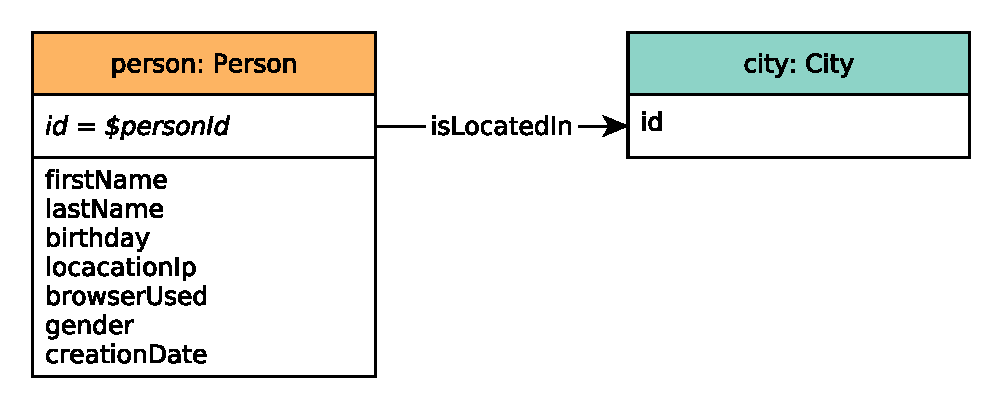
\includegraphics[scale=\patternscale,margin=0cm .2cm]{patterns/interactive-short-read-01}\hfill\vadjust{} \\ \hline
%
	desc. & Given a start Person, retrieve their first name, last name, birthday, IP
address, browser, and city of residence.
 \\ \hline
%
	
%
    
        params &
        \innerCardVSpace{\begin{tabularx}{\attributeCardWidth}{|>{\paramNumberCell}c|>{\varNameCell}M|>{\typeCell}m{\typeWidth}|Y|} \hline
        \cellcolor{parameter} \color{white} \footnotesize $\mathsf{1}$ &Person.id& ID &  \\ \hline
        \end{tabularx}}\innerCardVSpace \\ \hline
	
%
	
        result &
        \innerCardVSpace{\begin{tabularx}{\attributeCardWidth}{|>{\resultNumberCell}c|>{\varNameCell}M|>{\typeCell}m{\typeWidth}|>{\resultOriginCell}c|Y|} \hline
        $\mathsf{1}$ & Person.firstName & String &R&
                 \\ \hline
        $\mathsf{2}$ & Person.lastName & String &R&
                 \\ \hline
        $\mathsf{3}$ & Person.birthDay & Date &R&
                 \\ \hline
        $\mathsf{4}$ & Person.locationIP & String &R&
                 \\ \hline
        $\mathsf{5}$ & Person.browserUsed & String &R&
                 \\ \hline
        $\mathsf{6}$ & Person-isLocatedIn->Place.id & 32-bit Integer &R&
                 \\ \hline
        $\mathsf{7}$ & Person.gender & String &R&
                 \\ \hline
        $\mathsf{8}$ & Person.creationDate & DateTime &R&
                 \\ \hline
        \end{tabularx}}\innerCardVSpace \\ \hline
	
%
	%
	%
	%
    %
\end{tabularx}
\queryCardVSpace

\subsection{Update Query Descriptions}

\todo{Maybe introduce YAML specification for these as well?}
{\small
\begin{enumerate}
    \item Add Person
        \begin{itemize}
            \item \textbf{Description:} Add a Person to the social network.
            \item \textbf{Parameters:} \\
                \begin{tabular}{lll}
                    Person.id 	 			& ID & \parbox[t]{20cm}{\par \strut} \\
                    Person.firstName 		& String & \parbox[t]{20cm}{\par \strut} \\
                    Person.lastName 		& String & \parbox[t]{20cm}{\par \strut} \\
                    Person.gender 		& String & \parbox[t]{20cm}{\par \strut} \\
                    Person.birthDay 		& Date & \parbox[t]{20cm}{\par \strut} \\
                    Person.creationDate     & DateTime & \parbox[t]{20cm}{\par \strut} \\
                    Person.locationIp     & String & \parbox[t]{20cm}{\par \strut} \\
                    Person.browserUsed     & String & \parbox[t]{20cm}{\par \strut} \\
                    Person-isLocatedIn->City.id 	& ID & \parbox[t]{20cm}{\par \strut} \\
                    Person.speaks 	& \{ String \} & \parbox[t]{20cm}{\par \strut} \\
                    Person.emails 	& \{ String \} & \parbox[t]{20cm}{\par \strut} \\
                    Person-hasInterest->Tag.id 	& \{ ID \} & \parbox[t]{20cm}{\par \strut} \\
                    \{ Person-studyAt->University.id, \\
                    Person-studyAt->.classYear \}  & \{ID, 32-bit Integer\} & \parbox[t]{20cm}{\par \strut} \\
                        \{ Person-workAt->Company.id, \\
                        Person-workAt->.workFrom \}  & \{ID, 32-bit Integer\} & \parbox[t]{20cm}{\par \strut} \\
                        \end{tabular}
                \end{itemize}
            \item Add Post Like
                \begin{itemize}
                    \item \textbf{Description:} Add a Like to a Post of the social network.
                    \item \textbf{Parameters:} \\
                        \begin{tabular}{lll}
                            Person.id 	 			& ID & \parbox[t]{20cm}{\par \strut} \\
                            Post.id 	 			& ID & \parbox[t]{20cm}{\par \strut} \\
                            Person-likes->.creationDate 	 		& DateTime & \parbox[t]{20cm}{\par \strut} \\
                        \end{tabular}
                \end{itemize}
            \item Add Comment Like
                \begin{itemize}
                    \item \textbf{Description: Add a Like to a Comment of the social network.}
                    \item \textbf{Parameters:} \\
                        \begin{tabular}{lll}
                            Person.id 	 			& ID & \parbox[t]{20cm}{\par \strut} \\
                            Comment.id 	 			& ID & \parbox[t]{20cm}{\par \strut} \\
                            Person-likes->.creationDate 	 		& DateTime & \parbox[t]{20cm}{\par \strut} \\
                        \end{tabular}
                \end{itemize}
            \item Add Forum
                \begin{itemize}
                    \item \textbf{Description:} Add a Forum to the social network.
                    \item \textbf{Parameters:} \\
                        \begin{tabular}{lll}
                            Forum.id 	 			& ID & \parbox[t]{20cm}{// person 1\strut} \\
                            Forum.title 	 			& String & \parbox[t]{20cm}{// person 2\strut} \\
                            Forum.creationDate & DateTime & \parbox[t]{20cm}{\par \strut} \\
                            Forum-hasModerator->Person.id 	& \{ ID \} & \parbox[t]{20cm}{\par \strut} \\
                            Forum-hasTag->Tag.id 	& \{ ID \} & \parbox[t]{20cm}{\par \strut} \\
                        \end{tabular}
                \end{itemize}
            \item Add Forum Membership
                \begin{itemize}
                    \item \textbf{Description:} Add a Forum membership to the social network.
                    \item \textbf{Parameters:} \\
                        \begin{tabular}{lll}
                            Person.id 	 			& ID & \parbox[t]{20cm}{\par \strut} \\
                            Person-hasMember->Forum.id 	 			& ID & \parbox[t]{20cm}{\par \strut} \\
                            Person-hasMember->.joinDate 	 		& DateTime & \parbox[t]{20cm}{\par \strut} \\
                        \end{tabular}
                \end{itemize}
            \item Add Post
                \begin{itemize}
                    \item \textbf{Description:} Add a Post to the social network.
                    \item \textbf{Parameters:} \\
                        \begin{tabular}{lll}
                            Post.id 	 			& ID & \parbox[t]{20cm}{\par \strut} \\
                            Post.imageFile 	 			& String & \parbox[t]{20cm}{\par \strut} \\
                            Post.creationDate 	 		& DateTime & \parbox[t]{20cm}{\par \strut} \\
                            Post.locationIp 	 		& String & \parbox[t]{20cm}{\par \strut} \\
                            Post.browserUsed 	 		& String & \parbox[t]{20cm}{\par \strut} \\
                            Post.language 	 		    & String & \parbox[t]{20cm}{\par \strut} \\
                            Post.content 	 		    & Text & \parbox[t]{20cm}{\par \strut} \\
                            Post.length 	 		    & 32-bit Integer & \parbox[t]{20cm}{\par \strut} \\
                            Post-hasCreator->Person.id & ID & \parbox[t]{20cm}{\par \strut} \\
                            Forum-containerOf->Post.id & ID & \parbox[t]{20cm}{\par \strut} \\
                            Post-isLocatedIn->Country.id & ID & \parbox[t]{20cm}{\par \strut} \\
                            \{Post-hasTag->Tag.id\} & \{ID\} & \parbox[t]{20cm}{\par \strut} \\
                        \end{tabular}
                \end{itemize}
            \item Add Comment
                \begin{itemize}
                    \item \textbf{Description:} Add a Comment replying to a Post/Comment to the social network.
                    \item \textbf{Parameters:} \\
                        \begin{tabular}{lll}
                            Comment.id 	 			& ID & \parbox[t]{20cm}{\par \strut} \\
                            Comment.creationDate 			& DateTime & \parbox[t]{20cm}{\par \strut} \\
                            Comment.locationIp 	 		& String & \parbox[t]{20cm}{\par \strut} \\
                            Comment.browserUsed 	 		& String & \parbox[t]{20cm}{\par \strut} \\
                            Comment.content 	 		    & Text & \parbox[t]{20cm}{\par \strut} \\
                            Comment.length 	 		    & 32-bit Integer & \parbox[t]{20cm}{\par \strut} \\
                            Comment-hasCreator->Person.id & ID & \parbox[t]{20cm}{\par \strut} \\
                            Comment-isLocatedIn->Country.id & ID & \parbox[t]{20cm}{\par \strut} \\
                            Comment-replyOf->Post.id & ID & \parbox[t]{20cm}{ // -1 if the comment is a reply of a comment. \strut} \\
                            Comment-replyOf->Comment.id & ID & \parbox[t]{20cm}{// -1 if the comment is a reply of a post. \strut} \\
                            \{Comment-hasTag->Tag.id\} & \{ID\} & \parbox[t]{20cm}{\par \strut} \\
                        \end{tabular}
                \end{itemize}
            \item Add Friendship
                \begin{itemize}
                    \item \textbf{Description:} Add a friendship relation to the social network
                    \item \textbf{Parameters:} \\
                        \begin{tabular}{lll}
                            Person.id 	 			& ID & \parbox[t]{20cm}{// person 1\strut} \\
                            Person.id 	 			& ID & \parbox[t]{20cm}{// person 2\strut} \\
                            Person-knows->.creationDate & DateTime & \parbox[t]{20cm}{\par \strut} \\
                        \end{tabular}
                \end{itemize}
        \end{enumerate}
      }


\section{Substitution Parameters}

\input{interactive-parameters}

\section{Load Definition}


\input{interactive-workload}

\subsection{Business Intelligence Workload}
\subsubsection{Choke Points}

\subsubsection{Business Intelligence Queries}

{\small
    \begin{enumerate}
      \item Posting summary 
            \begin{itemize}
                \item \textbf{Description:}
                  Given a date, find all Messages (Posts and Comments) created before than that date.
                  Group them by a three level grouping.

                  \begin{itemize}
                    \item First: by their year of creation.
                    \item Second: for each year, group them into Posts and Comments.
                    \item Third: for each year-type (Post or Comment) group, split it into four groups based on the
                              length of their content: 
                              \begin{itemize}
                                \item if length is less than 40, it is 'short'; 
                                \item else, if length is less than 80, it is 'one liner';
                                \item else, if length is less than 160, it is 'tweet';
                                \item otherwise, it is 'long'
                              \end{itemize}
                  \end{itemize}

                \item \textbf{Parameters:} \\
                    \begin{tabular}{ll}
                      date 										& DateTime \\
                    \end{tabular}
                \item \textbf{Results:} \\
                  For every third-level group, return the the following aggregates:
                    \begin{tabular}{lll}
                      year 					& 32-bit Integer & \\
                      Message.type	& String & \parbox[t]{20cm}{// "Post" or "Comment"  \strut} \\
                      Message.length & 32-bit Integer & \\
                      category & 32-bit Integer & \parbox[t]{20cm}{// 0 (short), 1 (one-liner), 2 (tweet), 3 (long) \strut}  \\
                      count & 32-bit Integer &  \parbox[t]{20cm}{// The number of messages in this group  \strut} \\
                      average & 32-bit Integer &  \parbox[t]{20cm}{// The average Message length \strut} \\
                      sum & 32-bit Integer &  \parbox[t]{20cm}{// The sum of the Messages lengths \strut} \\
                      percentage & 32-bit Floating Point &  \parbox[t]{20cm}{// The percentage of Messages in this group
                        out of the total number \par of Messages created before the given date  \strut} \\
                      \end{tabular}
                    Sort the results first by Year (descending), then by the Message.type (Post 1st, or Comment 2nd) and
                    finally by the category (ascending)
                    \end{itemize}

      \item Top Tags from Country, age, gender and time 
            \begin{itemize}
                \item \textbf{Description:}
                  Select all Messages created between date1 and date2 (both included) by Persons located in any country
                  of a provided list of countries Select the creators (Persons) and the Tags of these Messages .  Split
                  these persons, tags and Messages into a five level grouping:
                  \begin{itemize}
                    \item First by the name of the country of the Person
                    \item  Second, by the month when the Message was created
                    \item Third, by the gender of the person
                    \item      Four, by the age group of the Person, which is defined as:
                      \begin{itemize}
                        \item The difference in years between the Person's birthday and the end of
                          simulation ('2013-01-01'), divided by 5, rounded down.
                      \end{itemize}
                    \item  Fifth, by the name of the tag attached to the Message
                  \end{itemize}
                \item \textbf{Parameters:} \\
                    \begin{tabular}{ll}
                      date1 & Date \\
                      date2 & Date \\
                      list of country names & \{String\} \\
                      endDate & Date \\
                    \end{tabular}
                \item \textbf{Results:} \\
                  For each of the fifth-level groups return: 
                    \begin{tabular}{lll}
                      Country.name & String & \\
                      month & 32-bit Integer & \\
                      gender & String & \parbox[t]{20cm}{// "Male" or "Female" \strut}\\
                      age group & 32-bit Integer & \\
                      Tag.name & String & \\
                      count & 32-bit Integer & \parbox[t]{20cm}{// The count of Messages falling in this group \strut}
                    \end{tabular}
                    Return top 100 groups where number of Messages is bigger than 100. Sort the groups by the count
                    (descending), Tag name (ascending), age group (ascending), gender (ascending), month
                    (ascending) and country name (ascending).
                    \end{itemize}
      \item Tag Evolution 
            \begin{itemize}
                \item \textbf{Description:}
                  Given two date intervals (left-closed, right-open), for each of these intervals find all Tags that
                  were used in Messages. For each interval, count the number of Messages containing each Tag.

                \item \textbf{Parameters:} \\
                    \begin{tabular}{ll}
                      dateStart1 & Date \\
                      dateEnd1 & Date \\
                      dateStart2 & Date \\
                      dateEnd2 & Date \\
                    \end{tabular}
                \item \textbf{Results:} \\
                  For each of the tags:
                    \begin{tabular}{lll}
                      Tag.name & String & \\
                      countInterval1 & 32-bit Integer & \parbox[t]{20cm}{// The number of occurrences of this Tag during
                        interval 1  \strut} \\
                      countInterval2 & 32-bit Integer & \parbox[t]{20cm}{// The number of occurrences of this Tag during
                        interval 2 \strut}\\
                      diff & 32-bit Integer & \parbox[t]{20cm}{ // The absolute difference countInterval1 and
                        countInterval2 \strut} \\
                    \end{tabular}
                    Return top-100 results sorted by the difference (descending) and then the tag name (ascending)
                    \end{itemize}

      \item Popular topics in a Country 
            \begin{itemize}
                \item \textbf{Description:}
                  Given a tagCalss and a Country, find all the Forums created in the given Country, containing at least
                  one Posts with Tags belonging directly to the given tagClass.
                  The location of a Forum is identified by the location of the Forum’s moderator.
                \item \textbf{Parameters:} \\
                    \begin{tabular}{ll}
                      TagClass.name & String \\
                      Country.name & String \\
                    \end{tabular}
                \item \textbf{Results:} \\
                  For each Forum:
                    \begin{tabular}{lll}
                      Forum.id  & ID & \\
                      Forum.title & String & \\
                      Forum.creationDate & DateTime & \\
                      Forum-hasModerator->Person.id & \{ ID \} & \\
                      count & 32-bit Integer &  \parbox[t]{20cm}{ // The number of Posts in the Forum with at least \par one Tag belonging to
                        the TagClass \strut} 
                    \end{tabular}
                    Return top-20 results sorted by count (descending) and Forum.id (ascending)
                    \end{itemize}

      \item Top posters in a Country 
            \begin{itemize}
                \item \textbf{Description:}
                  Find the most popular Forums for a given Country, where the popularity of a Forum is measured by the
                  number of members that Forum has from the given Country.  If multiple forums have the same member
                  count, use forum ID as tie breaker for popularity, where lower ID is more popular.  For each person
                  that is a member or moderator of any of the 100 most popular Forums, count the number of Posts they
                  made in any of those (most popular) Forums.

                  Group persons by:
                  \begin{itemize}
                      \item First, id
                      \item Second, first name
                      \item Third, last name
                      \item Fourth, creation date
                  \end{itemize}
                \item \textbf{Parameters:} \\
                    \begin{tabular}{ll}
                      Country.name & String \\ 
                    \end{tabular}
                \item \textbf{Results:} \\
                   For each group:
                    \begin{tabular}{lll}
                      Person.id & ID & \\
                      Person.firstName & String & \\
                      Person.lastName & String & \\
                      Person.creationDate & DateTime & \\
                      count & 32-bit Integer & \parbox[t]{20cm}{ // Number of Posts created by that Person \par in the top-100
                        most popular Forums\strut}  \\
                    \end{tabular}
                    Return top 100 Persons, sorted by count (descending) and by Person.Id (ascending).
                    \end{itemize}

      \item Most active posters on a given topic 
            \begin{itemize}
                \item \textbf{Description:}
                  Retrieve Persons who have created a Message with given Tag.  For each Person, compute a score as
                  follows: (the number of Messages they created that have given Tag) PLUS (2 x number of replies to
                  those Messages) PLUS (10 x number of Likes on those Messages).
                \item \textbf{Parameters:} \\
                    \begin{tabular}{ll}
                      Tag.name & 32-bit Integer 
                    \end{tabular}
                \item \textbf{Results:} \\
                  For each Person:
                    \begin{tabular}{lll}
                      Person.id & ID & \\
                      replyCount & 32-bit Integer & \parbox[t]{20cm}{ //The number of replies to Messages with
                        the \par given Tag created by the Person \strut}  \\
                      likeCount & 32-bit Integer & \parbox[t]{20cm}{ //The number of likes to Messages with
                        the \par given Tag created by the Person \strut}  \\ 
                      messageCount & 32-bit Integer & \parbox[t]{20cm}{ //The number of Messages with
                        the \par given Tag created by the Person \strut}  \\
                      score & 32-bit Integer & \\
                    \end{tabular}
                    Return the top-100 Persons, sorted by score (descending) and Person.id (ascending)
                    \end{itemize}

      \item Most authorative Person on a given topic 
            \begin{itemize}
                \item \textbf{Description:}
                  Given a Tag, find all Persons that ever created a Message with the given Tag.
                  For each of these Persons compute their "authority score".
                  The "authority score" for a given Person is defined as the sum of "popularity scores" of the Persons
                  that liked any of that Person's Messages with the given Tag.
                  A Person's "popularity score" is defined as the total number of likes on all of their Messages.
                \item \textbf{Parameters:} \\
                    \begin{tabular}{ll}
                      Tag.name & String \\
                    \end{tabular}
                \item \textbf{Results:} \\

                  For each Person:

                    \begin{tabular}{lll}
                      Person.Id & ID & \\
                      authorityScore & 32-bit Integer & \\
                    \end{tabular}

                    Return the top 100 Persons sorted the authorityScore (descending) and Person.Id (ascending).
                    \end{itemize}

      \item Related Topics 
            \begin{itemize}
                \item \textbf{Description:}
                  Find all Messages that have a given Tag.    
                  Find the Tags attached to replies of these Messages, but only those replies that do not have the given
                  Tag. Group the Tags by name, and get the count of replies in each group.
                \item \textbf{Parameters:} \\
                    \begin{tabular}{ll}
                      Tag.name & String \\
                    \end{tabular}
                \item \textbf{Results:} \\
                  For each group:
                    \begin{tabular}{lll}
                      Tag.name & String & \\
                      count & 32-bit Integer & \parbox[t]{20cm}{ // The count of replies with the Tag \strut} \\
                    \end{tabular}
                    Return the top-100 Tags, sorted by count (descending) and by Tag.name (ascending).
                    \end{itemize}

      \item Forum with related Tags 
            \begin{itemize}
                \item \textbf{Description:}
                  Given two tagClasses, find those forums that contain Posts with Tags belonging tagClass1 and contain
                  Posts with Tags belonging to tagCalss2 (not transitive). Consider the forums with a number of members
                  greater than a given threshold.
                  For every such forum, count the number of Posts  that have a Tag from tagclass t1 (count1), and the
                  number of posts that have a tag  from the tagclass2. 
                \item \textbf{Parameters:} \\
                    \begin{tabular}{ll}
                      TagClass1.name & String \\ 
                      TagClass2.name & String \\ 
                      threshold & 32-bit Integer \\
                    \end{tabular}
                \item \textbf{Results:} \\
                  For each Forum:
                    \begin{tabular}{lll}
                      Forum.id & ID & \\
                      count1 & 32-bit Integer & \parbox[t]{20cm}{ // The count of Posts with at least one Tag belonging
                        to TagClass1 \strut} \\
                      count2 & 32-bit Integer & \parbox[t]{20cm}{ // The count of Posts with at least one Tag belonging
                        to TagClass2 \strut} \\
                    \end{tabular}
                    \end{itemize}

      \item Central Person for a topic 
            \begin{itemize}
                \item \textbf{Description:}
                  Given a Tag, find all Persons that are either interested on the Tag, or have written a Post with the
                  given Tag. For each Person, compute the score as the sum of the following two aspects:

                  \begin{itemize}
                    \item 100, if the Person has this tag as their interest, or 0 otherwise
                    \item number of posts by this person with the given tag
                  \end{itemize}

                \item \textbf{Parameters:} \\
                    \begin{tabular}{ll}
                      Tag.name & String \\
                    \end{tabular}
                \item \textbf{Results:} \\
                  For each Person:

                    \begin{tabular}{lll}
                      Person.Id & ID & \\
                      score & 32-bit Integer & \\
                      friendsScore & 32-bit Integer & \parbox[t]{20cm}{ // The sum of the score of the Person's friends\strut} \\
                    \end{tabular}

                    Return the top-100 Persons, sorted the sum of score and friendsScore (descending), and  Person.id
                    (ascending) 
                \end{itemize}

      \item Tag Evolution 
            \begin{itemize}
                \item \textbf{Description:}
                \item \textbf{Parameters:} \\
                    \begin{tabular}{ll}
                    \end{tabular}
                \item \textbf{Results:} \\
                    \begin{tabular}{lll}
                    \end{tabular}
                    \end{itemize}
\end{enumerate}
}



\chapter{Interactive Workload}\label{section:workload}

\section{Query Specifications}

\subsection{Complex Reads Query Descriptions}

\renewcommand*{\arraystretch}{1.1}

\subsection*{Interactive / complex / 1}
\label{section:interactive-complex-read-01}

% change \emph{} to use sans-serif font
\let\oldemph\emph
\renewcommand{\emph}[1]{{\footnotesize \sf #1}}

\renewcommand{\currentQueryCard}{1}
\marginpar{
	\raggedleft
	\vspace{0.22ex}

	\queryRefCard{interactive-complex-read-01}{IC}{1}\\
	\queryRefCard{interactive-complex-read-02}{IC}{2}\\
	\queryRefCard{interactive-complex-read-03}{IC}{3}\\
	\queryRefCard{interactive-complex-read-04}{IC}{4}\\
	\queryRefCard{interactive-complex-read-05}{IC}{5}\\
	\queryRefCard{interactive-complex-read-06}{IC}{6}\\
	\queryRefCard{interactive-complex-read-07}{IC}{7}\\
	\queryRefCard{interactive-complex-read-08}{IC}{8}\\
	\queryRefCard{interactive-complex-read-09}{IC}{9}\\
	\queryRefCard{interactive-complex-read-10}{IC}{10}\\
	\queryRefCard{interactive-complex-read-11}{IC}{11}\\
	\queryRefCard{interactive-complex-read-12}{IC}{12}\\
	\queryRefCard{interactive-complex-read-13}{IC}{13}\\
	\queryRefCard{interactive-complex-read-14}{IC}{14}\\
}


\noindent\begin{tabularx}{\queryCardWidth}{|>{\queryPropertyCell}p{\queryPropertyCellWidth}|X|}
	\hline
	query & Interactive / complex / 1 \\ \hline
%
	title & Friends with certain name \\ \hline
%
	pattern & \multicolumn{1}{c|}{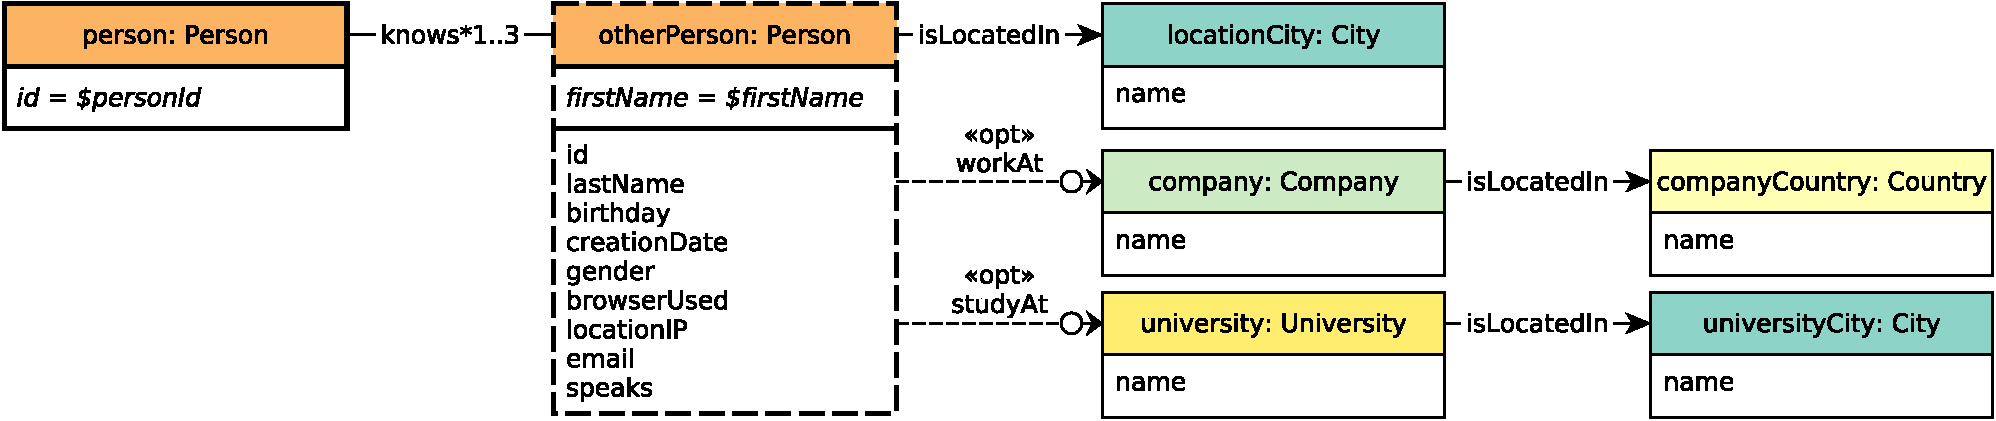
\includegraphics[scale=\patternscale,margin=0cm .2cm]{patterns/interactive-complex-read-01}} \\ \hline
%
	desc. & Given a start Person, find Persons with a given first name that the
start Person is connected to (excluding start Person) by at most 3 steps
via Knows relationships. Return Persons, including summaries of the
Persons workplaces and places of study.
 \\ \hline
%
	
		params &
		\innerCardVSpace{\begin{tabularx}{\attributeCardWidth}{|>{\paramNumberCell}c|>{\varNameCell}M|>{\typeCell}m{\typeWidth}|Y|} \hline
		$\mathsf{1}$ & Person.id
 & ID
 &  \\ \hline
		$\mathsf{2}$ & Person.firstName
 & String
 &  \\ \hline
		\end{tabularx}}\innerCardVSpace \\ \hline
	
%
	
		result &
		\innerCardVSpace{\begin{tabularx}{\attributeCardWidth}{|>{\resultNumberCell}c|>{\varNameCell}M|>{\typeCell}m{\typeWidth}|>{\resultOriginCell}c|Y|} \hline
		$\mathsf{1}$ & Person.id & ID & R &
				 \\ \hline
		$\mathsf{2}$ & Person.lastName & String & R &
				 \\ \hline
		$\mathsf{3}$ & distanceFromPerson & 32-bit Integer & R &
				1..3
 \\ \hline
		$\mathsf{4}$ & Person.birthday & Date & R &
				 \\ \hline
		$\mathsf{5}$ & Person.creationDate & DateTime & R &
				 \\ \hline
		$\mathsf{6}$ & Person.gender & String & R &
				 \\ \hline
		$\mathsf{7}$ & Person.browserUsed & String & R &
				 \\ \hline
		$\mathsf{8}$ & Person.locationIP & String & R &
				 \\ \hline
		$\mathsf{9}$ & \{Person.email\} & \{String\} & R &
				 \\ \hline
		$\mathsf{10}$ & \{Person.speaks\} & \{String\} & R &
				 \\ \hline
		$\mathsf{11}$ & Person-isLocatedIn-\textgreater{}Place.name & String & R &
				 \\ \hline
		$\mathsf{12}$ & \{Person-studyAt-\textgreater{}University.name,
Person-studyAt-\textgreater{}.classYear,
Person-studyAt-\textgreater{}University-isLocatedIn-\textgreater{}City.name\} & \{\textless{}String, 32-bit Integer, String\textgreater{}\} & R &
				 \\ \hline
		$\mathsf{13}$ & \{Person-workAt-\textgreater{}Company.name,
Person-workAt-\textgreater{}.workFrom,
Person-workAt-\textgreater{}Company-isLocatedIn-\textgreater{}Country.name\} & \{\textless{}String, 32-bit Integer, String\textgreater{}\} & R &
				 \\ \hline
		\end{tabularx}}\innerCardVSpace \\ \hline
	
%
	
		sort		&
		\innerCardVSpace{\begin{tabularx}{\attributeCardWidth}{|>{\sortNumberCell}c|>{\varNameCell}M|>{\directionCell}c|Y|} \hline
		$\mathsf{1}$ & distanceFromPerson
 & $\asc
$ &  \\ \hline
		$\mathsf{2}$ & Person.lastName
 & $\asc
$ &  \\ \hline
		$\mathsf{3}$ & Person.id
 & $\asc
$ &  \\ \hline
		\end{tabularx}}\innerCardVSpace \\ \hline
	%
	limit & 20 \\ \hline
	%
	CPs &
	\multicolumn{1}{>{\raggedright}l|}{
		\chokePoint{2.1}, 
		\chokePoint{5.3}
		} \\ \hline
	%
	relevance &
		\footnotesize This query is a representative of a simple navigational query. It looks for paths of length 1..3 through
the knows relation, starting from a given Person and ending at a Person with a given first name. It is interesting for several
aspects. (1) It requires for a complex aggregation for returning the concatenation of universities, companies,
languages and email information of the person. (2) It tests the ability of the optimizer to move the evaluation of
sub-queries functionally dependant on the Person, after the evaluation of the top-k. (3) Its performance is
highly sensitive to properly estimating the cardinalities in each transitive path, and paying attention not to explore
already visited Persons.
 \\ \hline%
\end{tabularx}
\queryCardVSpace

% change \emph back to the old one
\let\emph\oldemph
\renewcommand*{\arraystretch}{1.1}

\noindent\begin{tabularx}{17cm}{|>{\small \sf}c|X|}
	\hline
	query    & Interactive / complex / 2 \\ \hline
%
	title       & Recent posts and comments by your friends \\ \hline
%
    pattern     & \hfill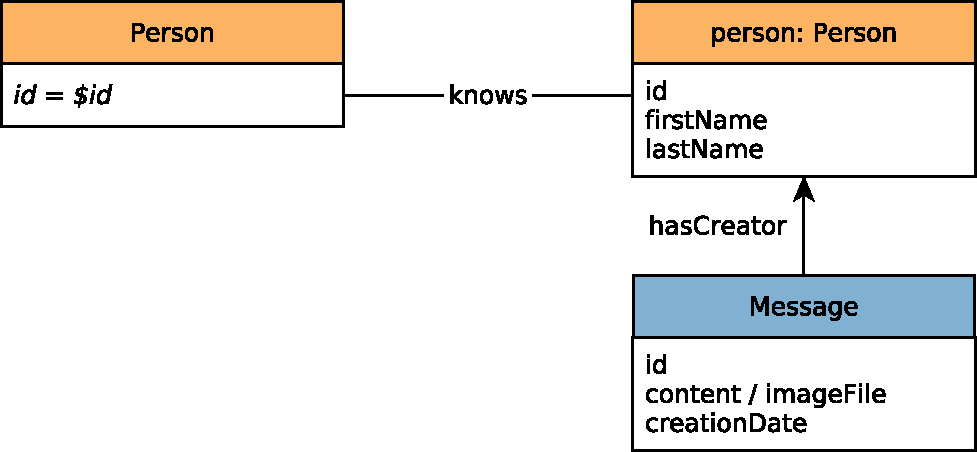
\includegraphics[scale=\patternscale,margin=0cm .2cm]{patterns/interactive-complex-read-02}\hfill\vadjust{} \\ \hline
%
	desc. & Given a start Person, find (most recent) Messages from all of that
Person's friends, that were created before (and including) a given date.
 \\ \hline
%
	
%
	params.  &
	\vspace{1.1ex}{\begin{tabularx}{14.2cm}{|c|M|m{2cm}|Y|} \hline
	\cellcolor{parameter} \color{white} $\mathsf{1}$ & \varname{Person.id} & \cellcolor{gray!20} \vartype{ID} &  \\ \hline
	\cellcolor{parameter} \color{white} $\mathsf{2}$ & \varname{date} & \cellcolor{gray!20} \vartype{DateTime} &  \\ \hline
	\end{tabularx}}\vspace{1.1ex} \\ \hline
%
	
	result      &
	\vspace{1.1ex}{\begin{tabularx}{14.2cm}{|c|M|m{2cm}|c|Y|} \hline
	\cellcolor{result} \color{white} $\mathsf{1}$ & \varname{Message-hasCreator->Person.id} & \cellcolor{gray!20} \vartype{ID} &
	    \texttt{R} &
	     \\ \hline
	\cellcolor{result} \color{white} $\mathsf{2}$ & \varname{Message-hasCreator->Person.firstName} & \cellcolor{gray!20} \vartype{String} &
	    \texttt{R} &
	     \\ \hline
	\cellcolor{result} \color{white} $\mathsf{3}$ & \varname{Message-hasCreator->Person.lastName} & \cellcolor{gray!20} \vartype{String} &
	    \texttt{R} &
	     \\ \hline
	\cellcolor{result} \color{white} $\mathsf{4}$ & \varname{Message.id} & \cellcolor{gray!20} \vartype{ID} &
	    \texttt{R} &
	     \\ \hline
	\cellcolor{result} \color{white} $\mathsf{5}$ & \varname{Message.content or Post.imageFile} & \cellcolor{gray!20} \vartype{String} &
	    \texttt{R} &
	     \\ \hline
	\cellcolor{result} \color{white} $\mathsf{6}$ & \varname{Message.creationDate} & \cellcolor{gray!20} \vartype{DateTime} &
	    \texttt{R} &
	     \\ \hline
	\end{tabularx}}\vspace{1.1ex} \\ \hline
	
%
	sort        &
	\vspace{1.1ex}{\begin{tabular}{|c|l|c|} \hline
	\cellcolor{sort} \color{white} $\mathsf{1}$ & \varname{Message.creationDate} & \cellcolor{gray!20} $\desc$ \\ \hline
	\cellcolor{sort} \color{white} $\mathsf{2}$ & \varname{Message.id} & \cellcolor{gray!20} $\asc$ \\ \hline
	\end{tabular}}\vspace{1.1ex} \\ \hline
	%
	limit       & 20 \\ \hline
	%
	CPs &
	\multicolumn{1}{>{\raggedright}l|}{
	  \chokepoint{1.1}, 
	  \chokepoint{2.2}, 
	  \chokepoint{2.3}, 
	  \chokepoint{3.2}
	  } \\ \hline
	%
    relevance &
      \small This is a navigational query looking for paths of length two, starting from a given Person, going to their friends and
from them, moving to their published Posts and Comments. This query exercices both the optimizer and how data is
stored. It tests the ability to create execution plans taking advantage of the orderings induced by some operators to
avoid performing expensive sorts. This query requires selecting Posts and Comments based on their creation date,
which might be correlated with their identifier and therefore, having intermediate results with interesting orders.
Also, messages could be stored in an order correlated with their creation date to improve data access locality. Finally,
as many of the attributes required in the projection are not needed for the execution of the query, it is expected that
the query optimizer will move the projection to the end.
 \\ \hline%
\end{tabularx}
\vspace{2ex}
\renewcommand*{\arraystretch}{1.1}

\noindent\begin{tabularx}{17cm}{|>{\small \sf}c|X|}
	\hline
	query    & Interactive / complex / 3 \\ \hline
%
	title       & Friends and friends of friends that have been to countries X and Y \\ \hline
%
    pattern     & \hfill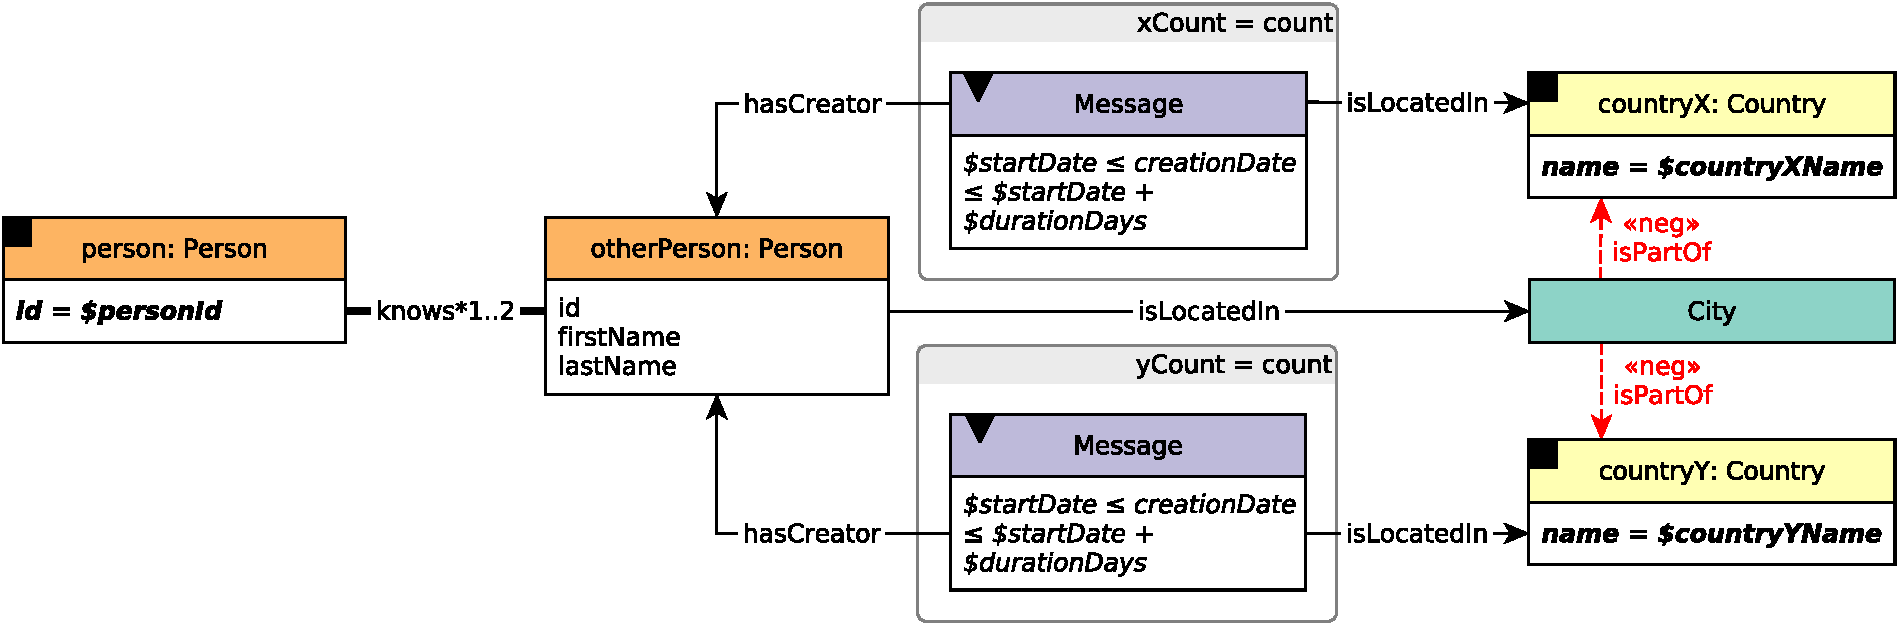
\includegraphics[scale=\patternscale,margin=0cm .2cm]{patterns/interactive-complex-read-03}\hfill\vadjust{} \\ \hline
%
	desc. & Given a start Person, find Persons that are their friends and friends of
friends (excluding start Person) that have made Posts/Comments in both
of the given Countries, X and Y, within a given period. Only Persons
that are foreign to Countries X and Y are considered, that is Persons
whose Location is not Country X or Country Y.
 \\ \hline
%
	
%
	params.  &
	\vspace{1.1ex}{\begin{tabularx}{14.66cm}{|c|M|m{2cm}|Y|} \hline
	\cellcolor{parameter} \color{white} $\mathsf{1}$ & \varname{Person.id} & \cellcolor{gray!20} \vartype{ID} &  \\ \hline
	\cellcolor{parameter} \color{white} $\mathsf{2}$ & \varname{CountryX.name} & \cellcolor{gray!20} \vartype{String} &  \\ \hline
	\cellcolor{parameter} \color{white} $\mathsf{3}$ & \varname{CountryY.name} & \cellcolor{gray!20} \vartype{String} &  \\ \hline
	\cellcolor{parameter} \color{white} $\mathsf{4}$ & \varname{startDate} & \cellcolor{gray!20} \vartype{Date} & beginning of requested period \\ \hline
	\cellcolor{parameter} \color{white} $\mathsf{5}$ & \varname{duration} & \cellcolor{gray!20} \vartype{32-bit Integer} & duration of requested period, in days the interval [startDate, startDate + Duration) is closed-open \\ \hline
	\end{tabularx}}\vspace{1.1ex} \\ \hline
%
	
	result      &
	\vspace{1.1ex}{\begin{tabularx}{14.66cm}{|c|M|m{2cm}|c|Y|} \hline
	\cellcolor{result} \color{white} $\mathsf{1}$ & \varname{Person.id} & \cellcolor{gray!20} \vartype{ID} &
	    \texttt{R} &
	     \\ \hline
	\cellcolor{result} \color{white} $\mathsf{2}$ & \varname{Person.firstName} & \cellcolor{gray!20} \vartype{String} &
	    \texttt{R} &
	     \\ \hline
	\cellcolor{result} \color{white} $\mathsf{3}$ & \varname{Person.lastName} & \cellcolor{gray!20} \vartype{String} &
	    \texttt{R} &
	     \\ \hline
	\cellcolor{result} \color{white} $\mathsf{4}$ & \varname{countX} & \cellcolor{gray!20} \vartype{32-bit Integer} &
	    \texttt{A} &
	    number of Messages from Country X made by Person within the given time \\ \hline
	\cellcolor{result} \color{white} $\mathsf{5}$ & \varname{countY} & \cellcolor{gray!20} \vartype{32-bit Integer} &
	    \texttt{A} &
	    number of Messages from Country Y made by Person within the given time \\ \hline
	\cellcolor{result} \color{white} $\mathsf{6}$ & \varname{count} & \cellcolor{gray!20} \vartype{32-bit Integer} &
	    \texttt{A} &
	    countX + countY \\ \hline
	\end{tabularx}}\vspace{1.1ex} \\ \hline
	
%
	sort        &
	\vspace{1.1ex}{\begin{tabular}{|c|l|c|} \hline
	\cellcolor{sort} \color{white} $\mathsf{1}$ & \varname{countX} & \cellcolor{gray!20} $\desc$ \\ \hline
	\cellcolor{sort} \color{white} $\mathsf{2}$ & \varname{Person.id} & \cellcolor{gray!20} $\asc$ \\ \hline
	\end{tabular}}\vspace{1.1ex} \\ \hline
	%
	limit       & 20 \\ \hline
	%
	CPs &
	\multicolumn{1}{>{\raggedright}l|}{
	  \chokepoint{2.1}, 
	  \chokepoint{3.1}, 
	  \chokepoint{5.1}
	  } \\ \hline
	%
    relevance &
      \small This query looks for paths of length two and three, starting from a Person, going to friends or friends of friends, and
then moving to Messages. This query tests the ability of the query optimizer to select the most efficient join ordering,
which will depend on the cardinalities of the intermediate results. Many friends of friends can be duplicate, then it is
expected to eliminate duplicates and those people prior to access the Post and Comments, as well as eliminate those
friends from countries X and Y, as the size of the intermediate results can be severely affected. A possible structural
optimization could be to materialize the number of Posts and Comments created by a person, and progressively
filter those people that could not even fall in the top 20 even having all their posts in the countries X and Y.
 \\ \hline%
\end{tabularx}
\vspace{2ex}
\renewcommand*{\arraystretch}{1.1}

\label{sec:interactive-complex-read-04}
\noindent\begin{tabularx}{\queryCardWidth}{|>{\queryPropertyCell}c|X|}
	\hline
	query & Interactive / complex / 4 \\ \hline
%
	title & New topics \\ \hline
%
    pattern & \hfill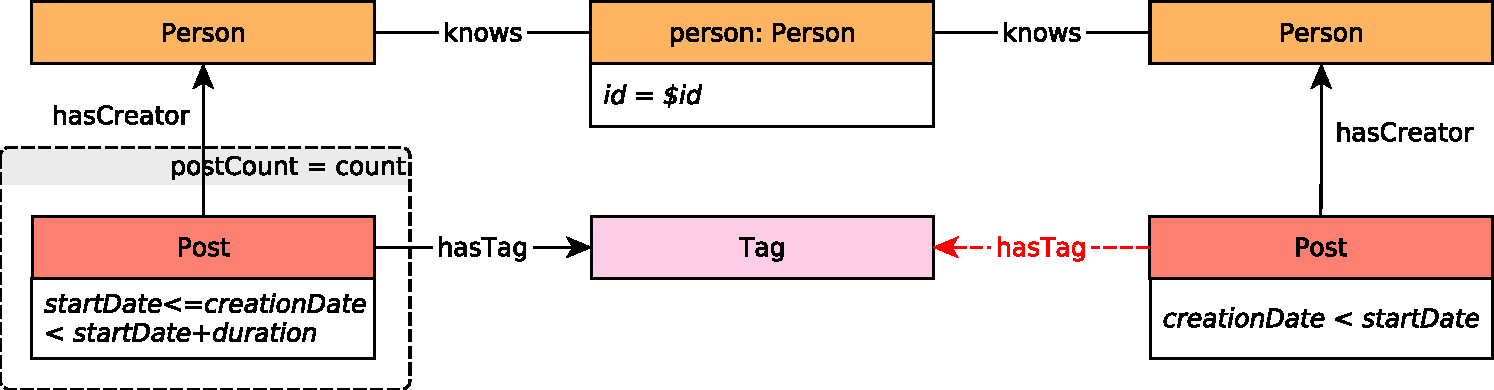
\includegraphics[scale=\patternscale,margin=0cm .2cm]{patterns/interactive-complex-read-04}\hfill\vadjust{} \\ \hline
%
	desc. & Given a start Person, find Tags that are attached to Posts that were
created by that Person's friends. Only include Tags that were attached
to friends' Posts created within a given time interval, and that were
never attached to friends' Posts created before this interval.
 \\ \hline
%
	
%
	params &
	\innerCardVSpace{\begin{tabularx}{\attributeCardWidth}{|>{\paramNumberCell}c|>{\varNameCell}M|>{\typeCell}m{\typeWidth}|Y|} \hline
	\cellcolor{parameter} \color{white} \footnotesize $\mathsf{1}$ &Person.id& ID &  \\ \hline
	\cellcolor{parameter} \color{white} \footnotesize $\mathsf{2}$ &startDate& Date &  \\ \hline
	\cellcolor{parameter} \color{white} \footnotesize $\mathsf{3}$ &duration& 32-bit Integer & duration of requested period, in days the interval [startDate, startDate + Duration) is closed-open \\ \hline
	\end{tabularx}}\innerCardVSpace \\ \hline
%
	
        result &
        \innerCardVSpace{\begin{tabularx}{\attributeCardWidth}{|>{\resultNumberCell}c|>{\varNameCell}M|>{\typeCell}m{\typeWidth}|>{\resultOriginCell}c|Y|} \hline
        $\mathsf{1}$ & Tag.name & String &R&
                 \\ \hline
        $\mathsf{2}$ & count & 32-bit Integer &A&
                number of Posts made within the given time interval that have this Tag \\ \hline
        \end{tabularx}}\innerCardVSpace \\ \hline
	
%
	sort        &
        \innerCardVSpace{\begin{tabular}{|>{\sortNumberCell}c|>{\varNameCell}l|>{\directionCell}c|} \hline
        $\mathsf{1}$ & count & $\desc$ \\ \hline
        $\mathsf{2}$ & Tag.name & $\asc$ \\ \hline
        \end{tabular}}\innerCardVSpace \\ \hline
	%
	limit & 10 \\ \hline
	%
	CPs &
	\multicolumn{1}{>{\raggedright}l|}{
	    \chokePoint{2.3}
	    } \\ \hline
	%
    relevance &
        \small This query looks for paths of length two, starting from a given Person, moving to Posts and then to Tags. It tests
the ability of the query optimizer to properly select the usage of hash joins or index based joins, depending on the
cardinality of the intermediate results. These cardinalities are clearly affected by the input Person, the number of
friends, the variety of Tags, the time interval and the number of Posts.
 \\ \hline%
\end{tabularx}
\queryCardVSpace
\renewcommand*{\arraystretch}{1.1}

\subsection*{Interactive / complex / 5}
\label{section:interactive-complex-read-05}

\noindent\begin{tabularx}{\queryCardWidth}{|>{\queryPropertyCell}p{\queryPropertyCellWidth}|X|}
	\hline
	query & Interactive / complex / 5 \\ \hline
%
	title & New groups
 \\ \hline
%
	pattern & \hfill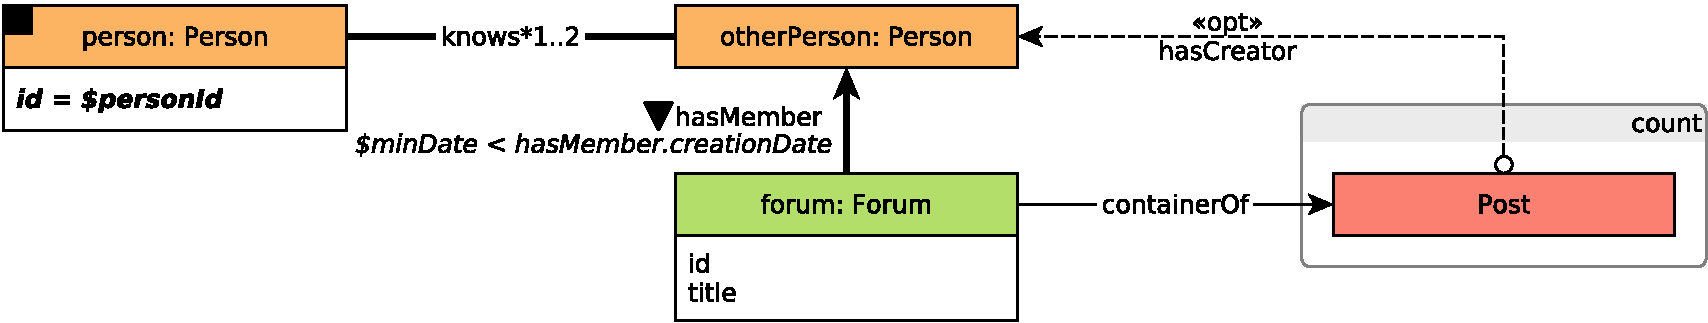
\includegraphics[scale=\patternscale,margin=0cm .2cm]{patterns/interactive-complex-read-05}\hfill\vadjust{} \\ \hline
%
	desc. & Given a start Person, find the Forums which that Person's friends and
friends of friends (excluding start Person) became Members of after a
given date. For each forum find the number of Posts that were created by
any of these Persons. For each Forum and consider only those Persons
which joined that particular Forum after the given date.
 \\ \hline
%
	
		params &
		\innerCardVSpace{\begin{tabularx}{\attributeCardWidth}{|>{\paramNumberCell}c|>{\varNameCell}M|>{\typeCell}m{\typeWidth}|Y|} \hline
		$\mathsf{1}$ & Person.id
 & ID
 &  \\ \hline
		$\mathsf{2}$ & date
 & Date
 &  \\ \hline
		\end{tabularx}}\innerCardVSpace \\ \hline
	
%
	
		result &
		\innerCardVSpace{\begin{tabularx}{\attributeCardWidth}{|>{\resultNumberCell}c|>{\varNameCell}M|>{\typeCell}m{\typeWidth}|>{\resultOriginCell}c|Y|} \hline
		$\mathsf{1}$ & Forum.title
 & String
 & R &
				 \\ \hline
		$\mathsf{2}$ & count
 & 32-bit Integer
 & R &
				Number of Posts made in Forum that were created by friends
 \\ \hline
		\end{tabularx}}\innerCardVSpace \\ \hline
	
%
	
		sort		&
		\innerCardVSpace{\begin{tabular}{|>{\sortNumberCell}c|>{\varNameCell}l|>{\directionCell}c|} \hline
		$\mathsf{1}$ & count
 & $\desc
$ \\ \hline
		$\mathsf{2}$ & Forum.id
 & $\asc
$ \\ \hline
		\end{tabular}}\innerCardVSpace \\ \hline
	%
	limit & 20 \\ \hline
	%
	CPs &
	\multicolumn{1}{>{\raggedright}l|}{
		\chokePoint{2.3}, 
		\chokePoint{3.3}
		} \\ \hline
	%
	relevance &
		\small This query looks for paths of length two and three, starting from a given Person, moving to friends and friends of
friends, and then getting the Forums they are members of. Besides testing the ability of the query optimizer to select
the proper join operator, it rewards the usage of indexes, but their accesses will be presumably scattered due to the
two/three-hop search space of the query, leading to unpredictable and scattered index accesses. Having efficient
implementations of such indexes will be highly beneficial.
 \\ \hline%
\end{tabularx}
\queryCardVSpace
\renewcommand*{\arraystretch}{1.1}

\subsection*{Interactive / complex / 6}
\label{section:interactive-complex-read-06}

% change \emph{} to use sans-serif font
\let\oldemph\emph
\renewcommand{\emph}[1]{{\footnotesize \sf #1}}

\renewcommand{\currentQueryCard}{6}
\marginpar{
	\raggedleft
	\vspace{0.22ex}

	\queryRefCard{interactive-complex-read-01}{IC}{1}\\
	\queryRefCard{interactive-complex-read-02}{IC}{2}\\
	\queryRefCard{interactive-complex-read-03}{IC}{3}\\
	\queryRefCard{interactive-complex-read-04}{IC}{4}\\
	\queryRefCard{interactive-complex-read-05}{IC}{5}\\
	\queryRefCard{interactive-complex-read-06}{IC}{6}\\
	\queryRefCard{interactive-complex-read-07}{IC}{7}\\
	\queryRefCard{interactive-complex-read-08}{IC}{8}\\
	\queryRefCard{interactive-complex-read-09}{IC}{9}\\
	\queryRefCard{interactive-complex-read-10}{IC}{10}\\
	\queryRefCard{interactive-complex-read-11}{IC}{11}\\
	\queryRefCard{interactive-complex-read-12}{IC}{12}\\
	\queryRefCard{interactive-complex-read-13}{IC}{13}\\
	\queryRefCard{interactive-complex-read-14}{IC}{14}\\
}


\noindent\begin{tabularx}{\queryCardWidth}{|>{\queryPropertyCell}p{\queryPropertyCellWidth}|X|}
	\hline
	query & Interactive / complex / 6 \\ \hline
%
	title & Tag co-occurrence \\ \hline
%
	pattern & \multicolumn{1}{c|}{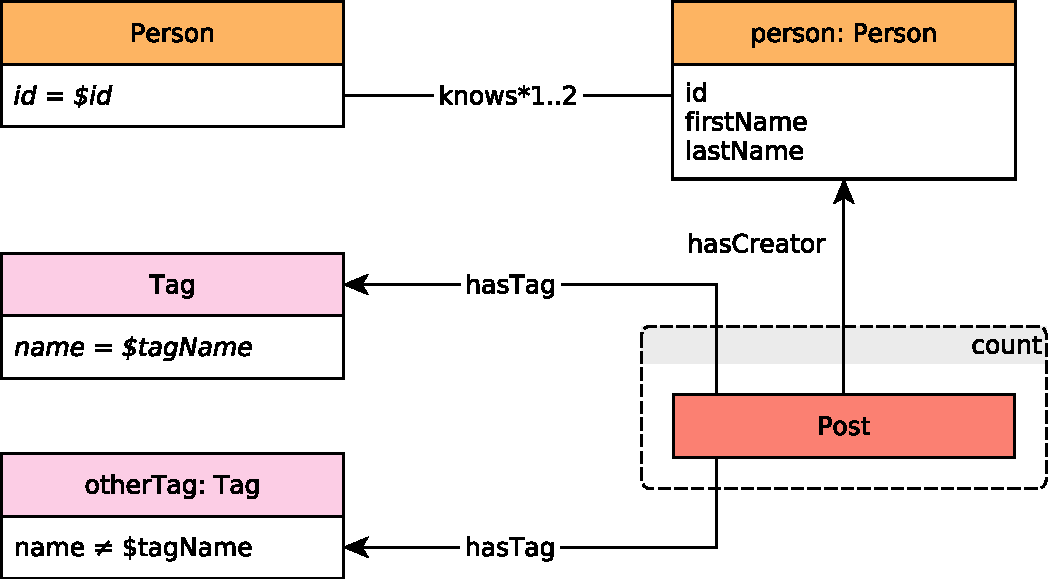
\includegraphics[scale=\patternscale,margin=0cm .2cm]{patterns/interactive-complex-read-06}} \\ \hline
%
	desc. & Given a start Person and some Tag, find the other Tags that occur
together with this Tag on Posts that were created by start Person's
friends and friends of friends (excluding start Person). Return For each
Tag, find the count of Posts that were created by these Persons, which
contain both this Tag and the given Tag.
 \\ \hline
%
	
		params &
		\innerCardVSpace{\begin{tabularx}{\attributeCardWidth}{|>{\paramNumberCell}c|>{\varNameCell}M|>{\typeCell}m{\typeWidth}|Y|} \hline
		$\mathsf{1}$ & Person.id
 & ID
 & \texttt{Person}
 \\ \hline
		$\mathsf{2}$ & Tag.name
 & String
 & \texttt{Tag}
 \\ \hline
		\end{tabularx}}\innerCardVSpace \\ \hline
	
%
	
		result &
		\innerCardVSpace{\begin{tabularx}{\attributeCardWidth}{|>{\resultNumberCell}c|>{\varNameCell}M|>{\typeCell}m{\typeWidth}|>{\resultOriginCell}c|Y|} \hline
		$\mathsf{1}$ & Tag.name & String & R &
				\texttt{tagName}
 \\ \hline
		$\mathsf{2}$ & postCount & 32-bit Integer & A &
				\texttt{postCount} -- Number of Posts that were created by friends and
friends of friends, which contain this Tag
 \\ \hline
		\end{tabularx}}\innerCardVSpace \\ \hline
	
%
	
		sort		&
		\innerCardVSpace{\begin{tabularx}{\attributeCardWidth}{|>{\sortNumberCell}c|>{\varNameCell}M|>{\directionCell}c|Y|} \hline
		$\mathsf{1}$ & postCount
 & $\desc
$ &  \\ \hline
		$\mathsf{2}$ & Tag.name
 & $\asc
$ &  \\ \hline
		\end{tabularx}}\innerCardVSpace \\ \hline
	%
	limit & 10 \\ \hline
	%
	CPs &
	\multicolumn{1}{>{\raggedright}l|}{
		\chokePoint{5.1}
		} \\ \hline
	%
	relevance &
		\footnotesize This query looks for paths of lengths three or four, starting from a Given Person, moving to friends or friends of
friends, then to Posts and finally ending at a given Tag.
 \\ \hline%
\end{tabularx}
\queryCardVSpace

% change \emph back to the old one
\let\emph\oldemph
\renewcommand*{\arraystretch}{1.1}

\subsection*{Interactive / complex / 7}
\label{section:interactive-complex-read-07}

% change \emph{} to use sans-serif font
\let\oldemph\emph
\renewcommand{\emph}[1]{{\footnotesize \sf #1}}

\renewcommand{\currentQueryCard}{7}
\marginpar{
	\raggedleft
	\vspace{0.22ex}

    \queryRefCard{interactive-complex-read-01}{IA}{1}\\
    \queryRefCard{interactive-complex-read-02}{IA}{2}\\
    \queryRefCard{interactive-complex-read-03}{IA}{3}\\
    \queryRefCard{interactive-complex-read-04}{IA}{4}\\
    \queryRefCard{interactive-complex-read-05}{IA}{5}\\
    \queryRefCard{interactive-complex-read-06}{IA}{6}\\
    \queryRefCard{interactive-complex-read-07}{IA}{7}\\
    \queryRefCard{interactive-complex-read-08}{IA}{8}\\
    \queryRefCard{interactive-complex-read-09}{IA}{9}\\
    \queryRefCard{interactive-complex-read-10}{IA}{10}\\
    \queryRefCard{interactive-complex-read-11}{IA}{11}\\
    \queryRefCard{interactive-complex-read-12}{IA}{12}\\
    \queryRefCard{interactive-complex-read-13}{IA}{13}\\
    \queryRefCard{interactive-complex-read-14}{IA}{14}\\
}


\noindent\begin{tabularx}{\queryCardWidth}{|>{\queryPropertyCell}p{\queryPropertyCellWidth}|X|}
	\hline
	query & Interactive / complex / 7 \\ \hline
%
	title & Recent likers
 \\ \hline
%
	pattern & \hfill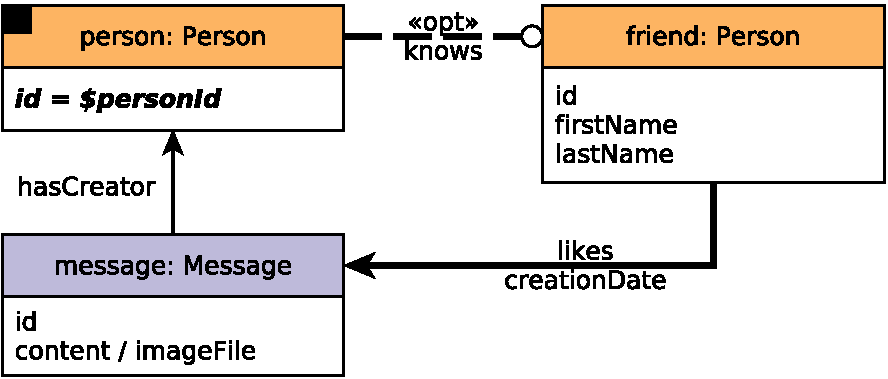
\includegraphics[scale=\patternscale,margin=0cm .2cm]{patterns/interactive-complex-read-07}\hfill\vadjust{} \\ \hline
%
	desc. & Given a start Person, find (most recent) Likes on any of start Person's
Messages. Find Persons that Liked any of start Person's Messages, the
Messages they liked most recently, creation date of that Like, and the
latency (in minutes) between creation of Messages and Like.
Additionally, for each Person found return a flag indicating whether the
liker is a friend of start Person. In the case that a Person Liked
multiple Messages at the same time, return the Message with lowest
identifier.
 \\ \hline
%
	
		params &
		\innerCardVSpace{\begin{tabularx}{\attributeCardWidth}{|>{\paramNumberCell}c|>{\varNameCell}M|>{\typeCell}m{\typeWidth}|Y|} \hline
		$\mathsf{1}$ & Person.id
 & 64-bit Integer
 &  \\ \hline
		\end{tabularx}}\innerCardVSpace \\ \hline
	
%
	
		result &
		\innerCardVSpace{\begin{tabularx}{\attributeCardWidth}{|>{\resultNumberCell}c|>{\varNameCell}M|>{\typeCell}m{\typeWidth}|>{\resultOriginCell}c|Y|} \hline
		$\mathsf{1}$ & Person.id & ID & R &
				 \\ \hline
		$\mathsf{2}$ & Person.firstName & String & R &
				 \\ \hline
		$\mathsf{3}$ & Person.lastName & String & R &
				 \\ \hline
		$\mathsf{4}$ & Like.creationDate & DateTime & R &
				 \\ \hline
		$\mathsf{5}$ & Message.id & ID & R &
				 \\ \hline
		$\mathsf{6}$ & Message.content or Post.imageFile & String & R &
				 \\ \hline
		$\mathsf{7}$ & latency & 32-bit Integer & C &
				Duration between creation of Message and Like, in minutes
 \\ \hline
		$\mathsf{8}$ & isNew & Boolean & C &
				\texttt{false} if liker Person is friend of start Person, \texttt{true}
otherwise
 \\ \hline
		\end{tabularx}}\innerCardVSpace \\ \hline
	
%
	
		sort		&
		\innerCardVSpace{\begin{tabularx}{\attributeCardWidth}{|>{\sortNumberCell}c|>{\varNameCell}M|>{\directionCell}c|Y|} \hline
		$\mathsf{1}$ & Like.creationDate
 & $\desc
$ &  \\ \hline
		$\mathsf{2}$ & Person.id
 & $\asc
$ &  \\ \hline
		\end{tabularx}}\innerCardVSpace \\ \hline
	%
	limit & 20 \\ \hline
	%
	CPs &
	\multicolumn{1}{>{\raggedright}l|}{
		\chokePoint{2.2}, 
		\chokePoint{2.3}, 
		\chokePoint{3.3}, 
		\chokePoint{5.1}
		} \\ \hline
	%
	relevance &
		\small This query looks for paths of length two, starting from a given Person, moving
to its published messages and then to Persons who liked them. It tests several aspects related to join optimization,
both at query optimization plan level and execution engine level. On the one hand, many of the columns needed for
the projection are only needed in the last stages of the query, so the optimizer is expected to delay the projection
until the end. This query implies accessing 2-hop data, and as a consequence, index accesses are expected to be
scattered. We expect to observe variate cardinalities, depending on the characteristics of the input parameter, so
properly selecting the join operators will be crucial. This query has a lot of correlated sub-queries, so it is testing
the ability to flatten the query execution plans.
 \\ \hline%
\end{tabularx}
\queryCardVSpace

% change \emph back to the old one
\renewcommand{\emph}[1]{\oldemph{#1}}
\renewcommand*{\arraystretch}{1.1}

\noindent\begin{tabularx}{17cm}{|p{1.95cm}|X|}
	\hline
	workload    & Interactive / complex \\ \hline
%
	query       & 8 \\ \hline
%
	title       & Recent replies \\ \hline
%
    pattern     & \hfill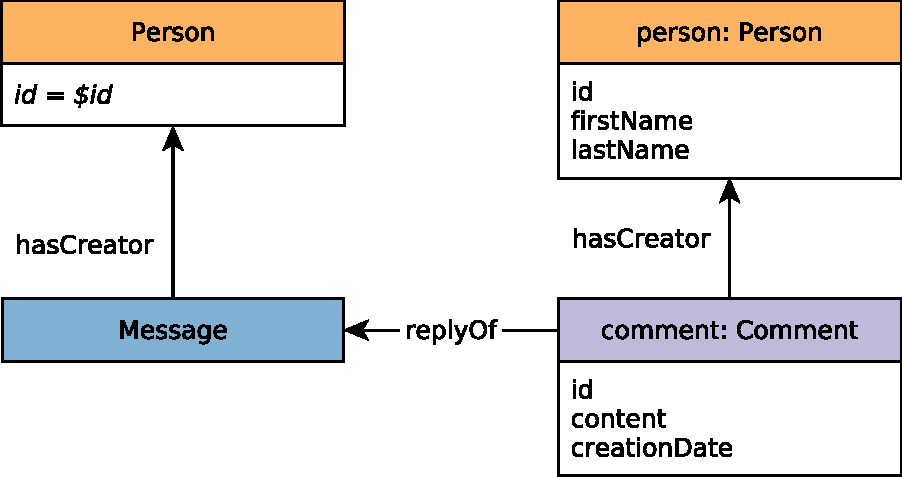
\includegraphics[scale=\patternscale,margin=0cm .2cm]{patterns/interactive-complex-read-08}\hfill\vadjust{} \\ \hline
%
	description & Given a start Person, find (most recent) Comments that are replies to
Messages of the start Person. Only consider immediate (1-hop) replies,
not the transitive (multi-hop) case. Return the reply Comments, and the
Person that created each reply Comment.
 \\ \hline
%
	
%
	parameters  &
	\vspace{1.1ex}{\begin{tabularx}{14.2cm}{|c|M|m{2cm}|Y|} \hline
	\cellcolor{parameter} \color{white} $\mathsf{1}$ & \varname{Person.id} & \cellcolor{gray!20} \vartype{ID} &  \\ \hline
	\end{tabularx}}\vspace{1.1ex} \\ \hline
%
	
	result      &
	\vspace{1.1ex}{\begin{tabularx}{14.2cm}{|c|M|m{2cm}|c|Y|} \hline
	\cellcolor{result} \color{white} $\mathsf{1}$ & \varname{Person.id} & \cellcolor{gray!20} \vartype{ID} &
	    \texttt{R} &
	     \\ \hline
	\cellcolor{result} \color{white} $\mathsf{2}$ & \varname{Person.firstName} & \cellcolor{gray!20} \vartype{String} &
	    \texttt{R} &
	     \\ \hline
	\cellcolor{result} \color{white} $\mathsf{3}$ & \varname{Person.lastName} & \cellcolor{gray!20} \vartype{String} &
	    \texttt{R} &
	     \\ \hline
	\cellcolor{result} \color{white} $\mathsf{4}$ & \varname{Comment.creationDate} & \cellcolor{gray!20} \vartype{DateTime} &
	    \texttt{R} &
	     \\ \hline
	\cellcolor{result} \color{white} $\mathsf{5}$ & \varname{Comment.id} & \cellcolor{gray!20} \vartype{ID} &
	    \texttt{R} &
	     \\ \hline
	\cellcolor{result} \color{white} $\mathsf{6}$ & \varname{Comment.content} & \cellcolor{gray!20} \vartype{String} &
	    \texttt{R} &
	     \\ \hline
	\end{tabularx}}\vspace{1.1ex} \\ \hline
	
%
	sort        &
	\vspace{1.1ex}{\begin{tabular}{|c|l|c|} \hline
	\cellcolor{sort} \color{white} $\mathsf{1}$ & \varname{Comment.creationDate} & \cellcolor{gray!20} $\desc$ \\ \hline
	\cellcolor{sort} \color{white} $\mathsf{2}$ & \varname{Comment.id} & \cellcolor{gray!20} $\asc$ \\ \hline
	\end{tabular}}\vspace{1.1ex} \\ \hline
	%
	limit       & 20 \\ \hline
	%
	%
\end{tabularx}
\vspace{2ex}
\renewcommand*{\arraystretch}{1.1}

\subsection*{Interactive / complex / 9}
\label{section:interactive-complex-read-09}

% change \emph{} to use sans-serif font
\let\oldemph\emph
\renewcommand{\emph}[1]{{\footnotesize \sf #1}}

\renewcommand{\currentQueryCard}{9}
\marginpar{
	\raggedleft
	\vspace{0.22ex}

	\queryRefCard{interactive-complex-read-01}{IC}{1}\\
	\queryRefCard{interactive-complex-read-02}{IC}{2}\\
	\queryRefCard{interactive-complex-read-03}{IC}{3}\\
	\queryRefCard{interactive-complex-read-04}{IC}{4}\\
	\queryRefCard{interactive-complex-read-05}{IC}{5}\\
	\queryRefCard{interactive-complex-read-06}{IC}{6}\\
	\queryRefCard{interactive-complex-read-07}{IC}{7}\\
	\queryRefCard{interactive-complex-read-08}{IC}{8}\\
	\queryRefCard{interactive-complex-read-09}{IC}{9}\\
	\queryRefCard{interactive-complex-read-10}{IC}{10}\\
	\queryRefCard{interactive-complex-read-11}{IC}{11}\\
	\queryRefCard{interactive-complex-read-12}{IC}{12}\\
	\queryRefCard{interactive-complex-read-13}{IC}{13}\\
	\queryRefCard{interactive-complex-read-14}{IC}{14}\\
}


\noindent\begin{tabularx}{\queryCardWidth}{|>{\queryPropertyCell}p{\queryPropertyCellWidth}|X|}
	\hline
	query & Interactive / complex / 9 \\ \hline
%
	title & Recent posts and comments by friends or friends of friends \\ \hline
%
	pattern & \multicolumn{1}{c|}{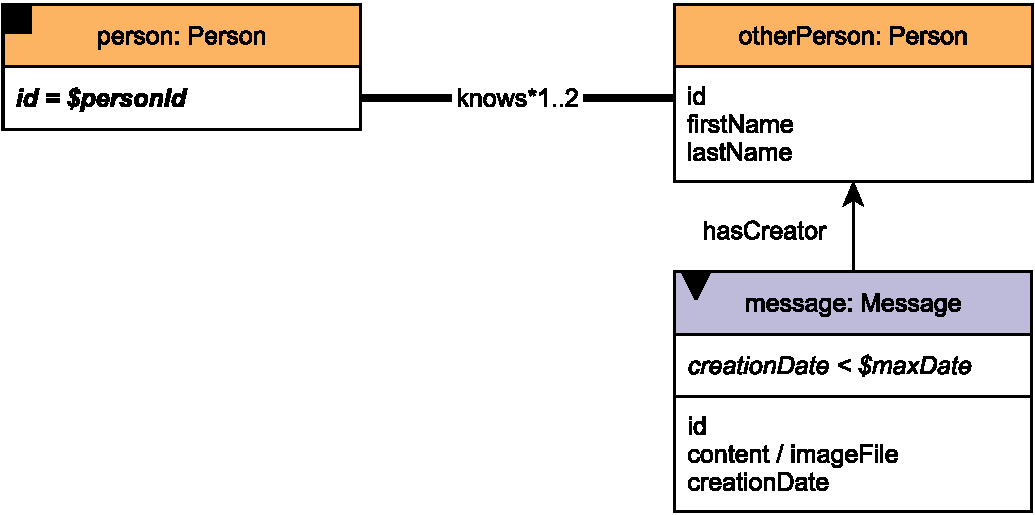
\includegraphics[scale=\patternscale,margin=0cm .2cm]{patterns/interactive-complex-read-09}} \\ \hline
%
	desc. & Given a start Person, find the (most recent) Messages created by that
Person's friends or friends of friends (excluding start Person). Only
consider the Messages created before a given date (excluding that date).
 \\ \hline
%
	
		params &
		\innerCardVSpace{\begin{tabularx}{\attributeCardWidth}{|>{\paramNumberCell}c|>{\varNameCell}M|>{\typeCell}m{\typeWidth}|Y|} \hline
		$\mathsf{1}$ & Person.id
 & ID
 &  \\ \hline
		$\mathsf{2}$ & date
 & Date
 &  \\ \hline
		\end{tabularx}}\innerCardVSpace \\ \hline
	
%
	
		result &
		\innerCardVSpace{\begin{tabularx}{\attributeCardWidth}{|>{\resultNumberCell}c|>{\varNameCell}M|>{\typeCell}m{\typeWidth}|>{\resultOriginCell}c|Y|} \hline
		$\mathsf{1}$ & Message-hasCreator-\textgreater{}Person.id & ID & R &
				\texttt{personId}
 \\ \hline
		$\mathsf{2}$ & Message-hasCreator-\textgreater{}Person.firstName & String & R &
				\texttt{personFirstName}
 \\ \hline
		$\mathsf{3}$ & Message-hasCreator-\textgreater{}Person.lastName & String & R &
				\texttt{personLastName}
 \\ \hline
		$\mathsf{4}$ & Message.id & ID & R &
				\texttt{commentOrPostId}
 \\ \hline
		$\mathsf{5}$ & Message.content or Post.imageFile & String & R &
				\texttt{commentOrPostContent}
 \\ \hline
		$\mathsf{6}$ & Message.creationDate & DateTime & R &
				\texttt{commentOrPostCreationDate}
 \\ \hline
		\end{tabularx}}\innerCardVSpace \\ \hline
	
%
	
		sort		&
		\innerCardVSpace{\begin{tabularx}{\attributeCardWidth}{|>{\sortNumberCell}c|>{\varNameCell}M|>{\directionCell}c|Y|} \hline
		$\mathsf{1}$ & Message.creationDate
 & $\desc
$ &  \\ \hline
		$\mathsf{2}$ & Message.id
 & $\asc
$ &  \\ \hline
		\end{tabularx}}\innerCardVSpace \\ \hline
	%
	limit & 20 \\ \hline
	%
	CPs &
	\multicolumn{1}{>{\raggedright}l|}{
		\chokePoint{1.1}, 
		\chokePoint{1.2}, 
		\chokePoint{2.2}, 
		\chokePoint{2.3}, 
		\chokePoint{3.2}, 
		\chokePoint{3.3}
		} \\ \hline
	%
	relevance &
		\footnotesize This query looks for paths of length two or three, starting from a given Person, moving to its friends and friends of
friends, and ending at their created Messages. This is one of the most complex queries, as the list of choke-points
indicates. This query is expected to touch variable amounts of data with entities of different characteristics, and
therefore, properly estimating cardinalities and selecting the proper operators will be crucial.
 \\ \hline%
\end{tabularx}
\queryCardVSpace

% change \emph back to the old one
\let\emph\oldemph
\renewcommand*{\arraystretch}{1.1}

\subsection*{Interactive / complex / 10}
\label{section:interactive-complex-read-10}

% change \emph{} to use sans-serif font
\let\oldemph\emph
\renewcommand{\emph}[1]{{\footnotesize \sf #1}}

\renewcommand{\currentQueryCard}{10}
\marginpar{
	\raggedleft
	\vspace{0.22ex}

	\queryRefCard{interactive-complex-read-01}{IC}{1}\\
	\queryRefCard{interactive-complex-read-02}{IC}{2}\\
	\queryRefCard{interactive-complex-read-03}{IC}{3}\\
	\queryRefCard{interactive-complex-read-04}{IC}{4}\\
	\queryRefCard{interactive-complex-read-05}{IC}{5}\\
	\queryRefCard{interactive-complex-read-06}{IC}{6}\\
	\queryRefCard{interactive-complex-read-07}{IC}{7}\\
	\queryRefCard{interactive-complex-read-08}{IC}{8}\\
	\queryRefCard{interactive-complex-read-09}{IC}{9}\\
	\queryRefCard{interactive-complex-read-10}{IC}{10}\\
	\queryRefCard{interactive-complex-read-11}{IC}{11}\\
	\queryRefCard{interactive-complex-read-12}{IC}{12}\\
	\queryRefCard{interactive-complex-read-13}{IC}{13}\\
	\queryRefCard{interactive-complex-read-14}{IC}{14}\\
}


\noindent\begin{tabularx}{\queryCardWidth}{|>{\queryPropertyCell}p{\queryPropertyCellWidth}|X|}
	\hline
	query & Interactive / complex / 10 \\ \hline
%
	title & Friend recommendation \\ \hline
%
	pattern & \multicolumn{1}{c|}{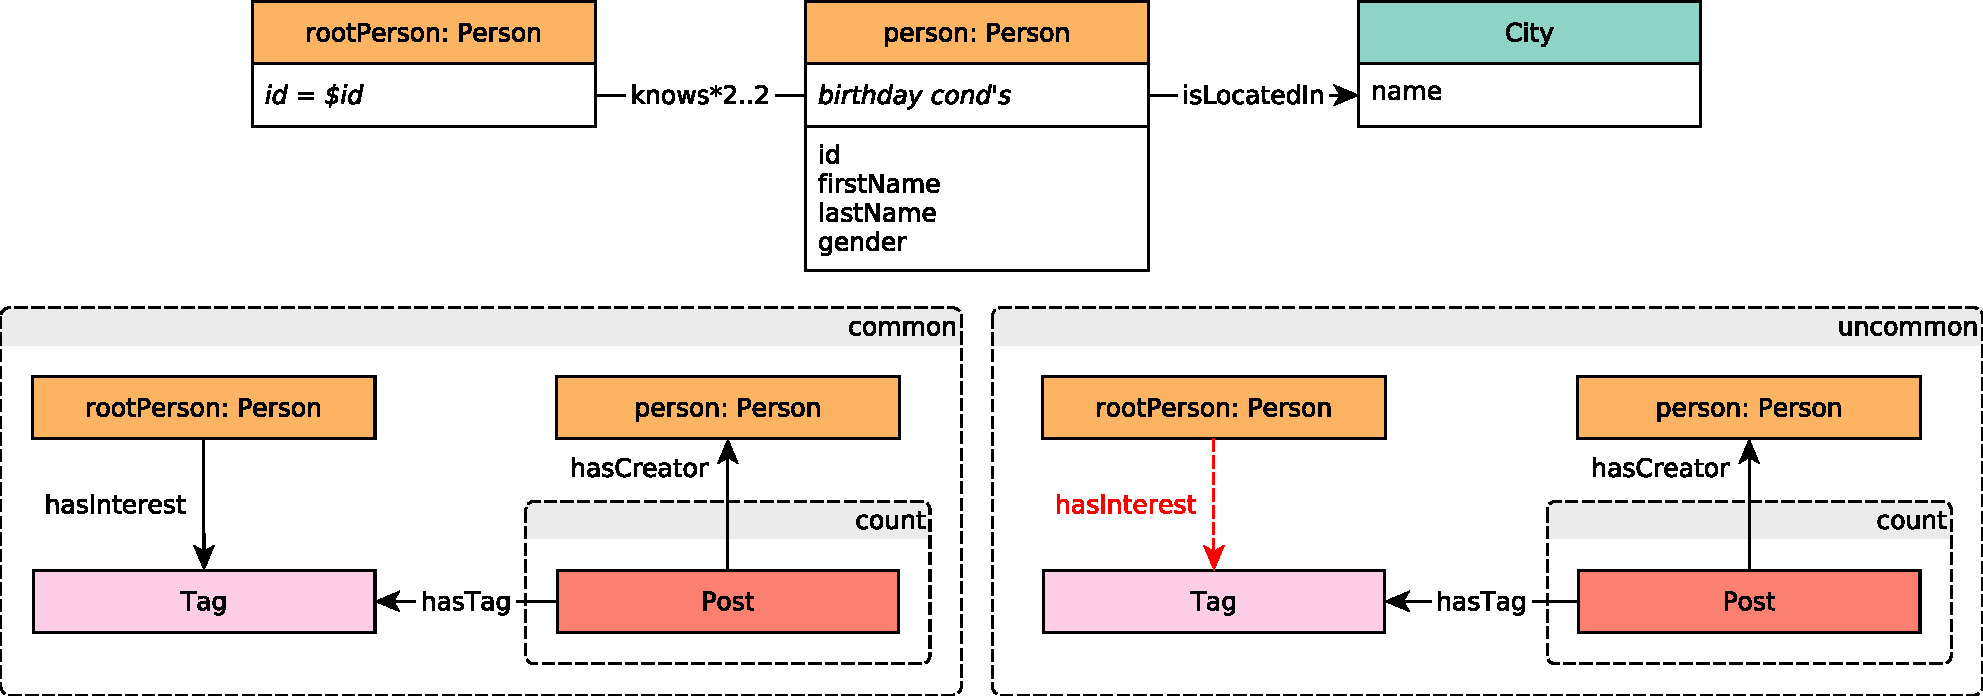
\includegraphics[scale=\patternscale,margin=0cm .2cm]{patterns/interactive-complex-read-10}} \\ \hline
%
	desc. & Given a start Person, find that Person's friends of friends (excluding
start Person, and immediate friends), who were born on or after the 21st
of a given month (in any year) and before the 22nd of the following
month. Calculate the similarity between each of these Persons and start
Person, where similarity for any Person is defined as follows:

\begin{itemize}
\tightlist
\item
  common = number of Posts created by that Person, such that the Post
  has a Tag that start Person is Interested in
\item
  uncommon = number of Posts created by that Person, such that the Post
  has no Tag that start Person is Interested in
\item
  similarity = common - uncommon
\end{itemize}
 \\ \hline
%
	
		params &
		\innerCardVSpace{\begin{tabularx}{\attributeCardWidth}{|>{\paramNumberCell}c|>{\varNameCell}M|>{\typeCell}m{\typeWidth}|Y|} \hline
		$\mathsf{1}$ & Person.id
 & ID
 &  \\ \hline
		$\mathsf{2}$ & month
 & 32-bit Integer
 & Between 1-12
 \\ \hline
		\end{tabularx}}\innerCardVSpace \\ \hline
	
%
	
		result &
		\innerCardVSpace{\begin{tabularx}{\attributeCardWidth}{|>{\resultNumberCell}c|>{\varNameCell}M|>{\typeCell}m{\typeWidth}|>{\resultOriginCell}c|Y|} \hline
		$\mathsf{1}$ & Person.id & ID & R &
				 \\ \hline
		$\mathsf{2}$ & Person.firstName & String & R &
				 \\ \hline
		$\mathsf{3}$ & Person.lastName & String & R &
				 \\ \hline
		$\mathsf{4}$ & similarity & 32-bit Integer & C &
				 \\ \hline
		$\mathsf{5}$ & Person.gender & String & R &
				 \\ \hline
		$\mathsf{6}$ & Person-isLocatedIn-\textgreater{}Place.name & String & R &
				 \\ \hline
		\end{tabularx}}\innerCardVSpace \\ \hline
	
%
	
		sort		&
		\innerCardVSpace{\begin{tabularx}{\attributeCardWidth}{|>{\sortNumberCell}c|>{\varNameCell}M|>{\directionCell}c|Y|} \hline
		$\mathsf{1}$ & similarity
 & $\desc
$ &  \\ \hline
		$\mathsf{2}$ & Person.id
 & $\asc
$ &  \\ \hline
		\end{tabularx}}\innerCardVSpace \\ \hline
	%
	limit & 10 \\ \hline
	%
	CPs &
	\multicolumn{1}{>{\raggedright}l|}{
		\chokePoint{2.3}, 
		\chokePoint{3.3}, 
		\chokePoint{4.1}, 
		\chokePoint{4.2}, 
		\chokePoint{5.1}, 
		\chokePoint{5.2}, 
		\chokePoint{6.1}, 
		\chokePoint{7.1}
		} \\ \hline
	%
	relevance &
		\footnotesize This query looks for paths of length two, starting from a Person and ending at the friends of their friends. It does
widely scattered graph traversal, and one expects no locality of in friends of friends, as these have been acquired
over a long time and have widely scattered identifiers. The join order is simple but one must see that the anti-join
for "not in my friends" is better with hash. Also the last pattern in the scalar sub-queries joining or anti-joining the
tags of the candidate's posts to interests of self should be by hash.
 \\ \hline%
\end{tabularx}
\queryCardVSpace

% change \emph back to the old one
\let\emph\oldemph
\renewcommand*{\arraystretch}{1.1}

\subsection*{Interactive / complex / 11}
\label{section:interactive-complex-read-11}

\noindent\begin{tabularx}{\queryCardWidth}{|>{\queryPropertyCell}p{\queryPropertyCellWidth}|X|}
	\hline
	query & Interactive / complex / 11 \\ \hline
%
	title & Job referral
 \\ \hline
%
	pattern & \hfill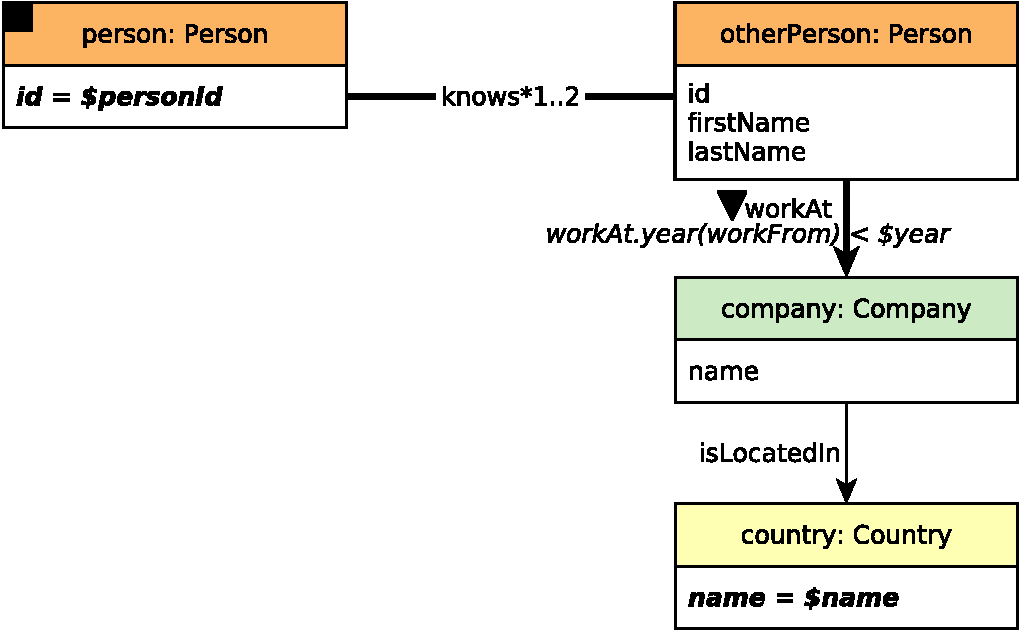
\includegraphics[scale=\patternscale,margin=0cm .2cm]{patterns/interactive-complex-read-11}\hfill\vadjust{} \\ \hline
%
	desc. & Given a start Person, find that Person's friends and friends of friends
(excluding start Person) who started Working in some Company in a given
Country, before a given date (year).
 \\ \hline
%
	
		params &
		\innerCardVSpace{\begin{tabularx}{\attributeCardWidth}{|>{\paramNumberCell}c|>{\varNameCell}M|>{\typeCell}m{\typeWidth}|Y|} \hline
		$\mathsf{1}$ & Person.id
 & ID
 &  \\ \hline
		$\mathsf{2}$ & Country.name
 & String
 &  \\ \hline
		$\mathsf{3}$ & year
 & 32-bit Integer
 &  \\ \hline
		\end{tabularx}}\innerCardVSpace \\ \hline
	
%
	
		result &
		\innerCardVSpace{\begin{tabularx}{\attributeCardWidth}{|>{\resultNumberCell}c|>{\varNameCell}M|>{\typeCell}m{\typeWidth}|>{\resultOriginCell}c|Y|} \hline
		$\mathsf{1}$ & Person.id
 & ID
 & R &
				 \\ \hline
		$\mathsf{2}$ & Person.firstName
 & String
 & R &
				 \\ \hline
		$\mathsf{3}$ & Person.lastName
 & String
 & R &
				 \\ \hline
		$\mathsf{4}$ & Person-worksAt-\textgreater{}Organisation.name
 & String
 & R &
				 \\ \hline
		$\mathsf{5}$ & Person-worksAt-\textgreater{}.worksFrom
 & 32-bit Integer
 & R &
				 \\ \hline
		\end{tabularx}}\innerCardVSpace \\ \hline
	
%
	
		sort		&
		\innerCardVSpace{\begin{tabularx}{\attributeCardWidth}{|>{\sortNumberCell}c|>{\varNameCell}M|>{\directionCell}c|Y|} \hline
		$\mathsf{1}$ & Person-worksAt-\textgreater{}.worksFrom
 & $\asc
$ &  \\ \hline
		$\mathsf{2}$ & Person.id
 & $\asc
$ &  \\ \hline
		$\mathsf{3}$ & Person-worksAt-\textgreater{}Organisation.name
 & $\desc
$ &  \\ \hline
		\end{tabularx}}\innerCardVSpace \\ \hline
	%
	limit & 10 \\ \hline
	%
	CPs &
	\multicolumn{1}{>{\raggedright}l|}{
		\chokePoint{1.4}, 
		\chokePoint{2.3}, 
		\chokePoint{2.4}, 
		\chokePoint{3.3}
		} \\ \hline
	%
	relevance &
		\small This query looks for paths of length two or three, starting from a Person, moving to friends or friends of friends,
and ending at a Company. In this query, there are selective joins and a top k order by that can be exploited for
optimizations.
 \\ \hline%
\end{tabularx}
\queryCardVSpace
\renewcommand*{\arraystretch}{1.1}

\subsection*{Interactive / complex / 12}
\label{section:interactive-complex-read-12}

% change \emph{} to use sans-serif font
\let\oldemph\emph
\renewcommand{\emph}[1]{{\footnotesize \sf #1}}

\renewcommand{\currentQueryCard}{12}
\marginpar{
	\raggedleft
	\vspace{0.22ex}

	\queryRefCard{interactive-complex-read-01}{IC}{1}\\
	\queryRefCard{interactive-complex-read-02}{IC}{2}\\
	\queryRefCard{interactive-complex-read-03}{IC}{3}\\
	\queryRefCard{interactive-complex-read-04}{IC}{4}\\
	\queryRefCard{interactive-complex-read-05}{IC}{5}\\
	\queryRefCard{interactive-complex-read-06}{IC}{6}\\
	\queryRefCard{interactive-complex-read-07}{IC}{7}\\
	\queryRefCard{interactive-complex-read-08}{IC}{8}\\
	\queryRefCard{interactive-complex-read-09}{IC}{9}\\
	\queryRefCard{interactive-complex-read-10}{IC}{10}\\
	\queryRefCard{interactive-complex-read-11}{IC}{11}\\
	\queryRefCard{interactive-complex-read-12}{IC}{12}\\
	\queryRefCard{interactive-complex-read-13}{IC}{13}\\
	\queryRefCard{interactive-complex-read-14}{IC}{14}\\
}


\noindent\begin{tabularx}{\queryCardWidth}{|>{\queryPropertyCell}p{\queryPropertyCellWidth}|X|}
	\hline
	query & Interactive / complex / 12 \\ \hline
%
	title & Expert search \\ \hline
%
	pattern & \centering 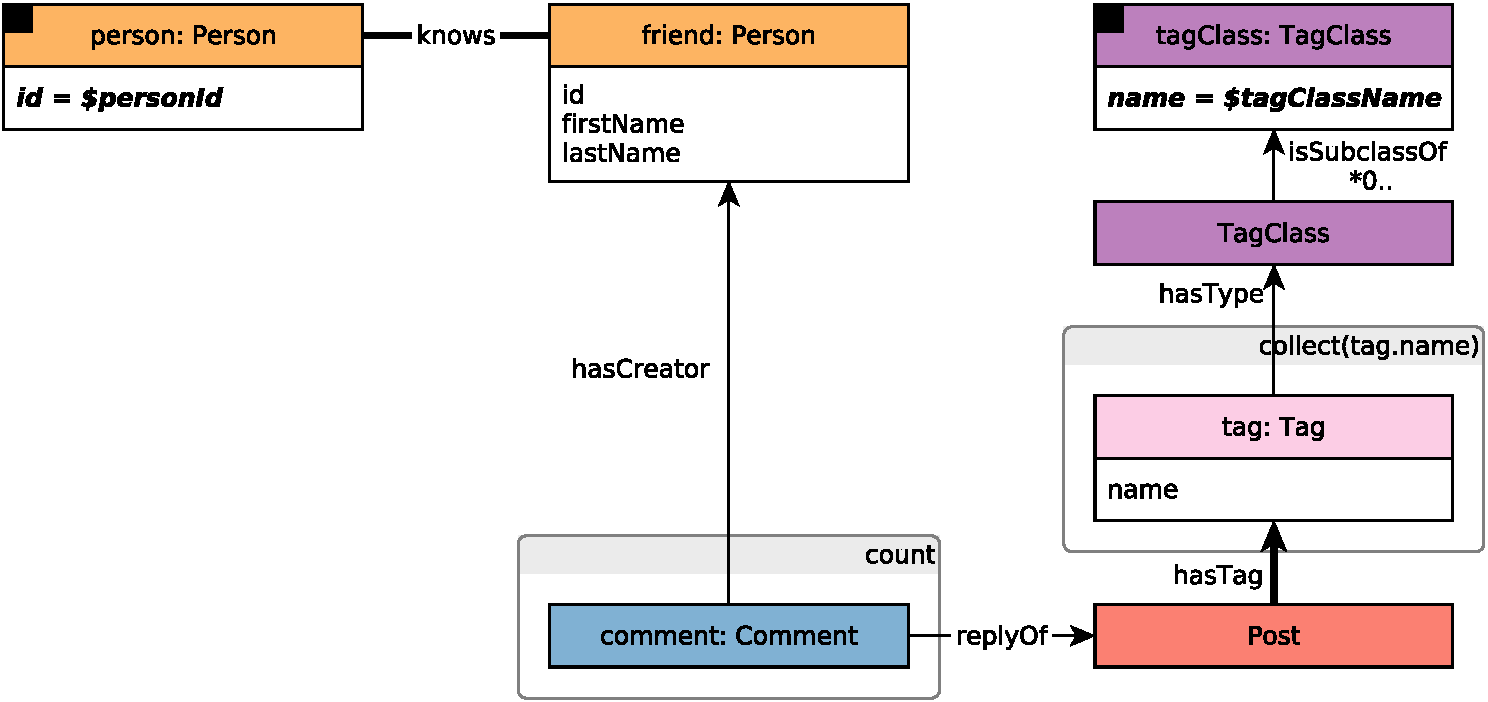
\includegraphics[scale=\patternscale,margin=0cm .2cm]{patterns/interactive-complex-read-12} \tabularnewline \hline
%
	desc. & Given a start Person, find the Comments that this Person's friends made
in reply to Posts, considering only those Comments that are immediate
(1-hop) replies to Posts, not the transitive (multi-hop) case. Only
consider Posts with a Tag in a given TagClass or in a descendent of that
TagClass. Count the number of these reply Comments, and collect the Tags
that were attached to the Posts they replied to, but only collect Tags
with the given TagClass or with a descendant of that TagClass Return
Persons with at least one reply, the reply count, and the collection of
Tags.
 \\ \hline
%
	
		params &
		\innerCardVSpace{\begin{tabularx}{\attributeCardWidth}{|>{\paramNumberCell}c|>{\varNameCell}M|>{\typeCell}m{\typeWidth}|Y|} \hline
		$\mathsf{1}$ & Person.id
 & ID
 & \texttt{personId}
 \\ \hline
		$\mathsf{2}$ & TagClass.name
 & String
 & \texttt{tagClassName}
 \\ \hline
		\end{tabularx}}\innerCardVSpace \\ \hline
	
%
	
		result &
		\innerCardVSpace{\begin{tabularx}{\attributeCardWidth}{|>{\resultNumberCell}c|>{\varNameCell}M|>{\typeCell}m{\typeWidth}|>{\resultOriginCell}c|Y|} \hline
		$\mathsf{1}$ & Person.id & ID & R &
				\texttt{personId}
 \\ \hline
		$\mathsf{2}$ & Person.firstName & String & R &
				\texttt{personFirstName}
 \\ \hline
		$\mathsf{3}$ & Person.lastName & String & R &
				\texttt{personLastName}
 \\ \hline
		$\mathsf{4}$ & \{Tag.name\} & \{String\} & R &
				\texttt{tagNames}
 \\ \hline
		$\mathsf{5}$ & replyCount & 32-bit Integer & A &
				\texttt{replyCount} -- Number of reply Comments
 \\ \hline
		\end{tabularx}}\innerCardVSpace \\ \hline
	
%
	
		sort		&
		\innerCardVSpace{\begin{tabularx}{\attributeCardWidth}{|>{\sortNumberCell}c|>{\varNameCell}M|>{\directionCell}c|Y|} \hline
		$\mathsf{1}$ & count
 & $\desc
$ &  \\ \hline
		$\mathsf{2}$ & Person.id
 & $\asc
$ &  \\ \hline
		\end{tabularx}}\innerCardVSpace \\ \hline
	%
	limit & 20 \\ \hline
	%
	CPs &
	\multicolumn{1}{>{\raggedright}l|}{
		\chokePoint{3.3}, 
		\chokePoint{7.2}, 
		\chokePoint{7.3}, 
		\chokePoint{8.2}
		} \\ \hline
	%
	relevance &
		\footnotesize This query looks for paths of length three, starting at a Person, moving to its friends, the to their Comments and
ending at the Post the Comments are replying. The chain from original post to the reply is transitive. The traversal
may be initiated at either end, the system may note that this is a tree, hence leaf to root is always best. Additionally,
a hash table can be built from either end, e.g. from the friends of self, from the tags in the category, from the or
other.
 \\ \hline%
\end{tabularx}
\queryCardVSpace

% change \emph back to the old one
\let\emph\oldemph
\renewcommand*{\arraystretch}{1.1}

\subsection*{Interactive / complex / 13}
\label{section:interactive-complex-read-13}

% change \emph{} to use sans-serif font
\let\oldemph\emph
\renewcommand{\emph}[1]{{\footnotesize \sf #1}}

\renewcommand{\currentQueryCard}{13}
\marginpar{
	\raggedleft
	\vspace{0.22ex}

	\queryRefCard{interactive-complex-read-01}{IC}{1}\\
	\queryRefCard{interactive-complex-read-02}{IC}{2}\\
	\queryRefCard{interactive-complex-read-03}{IC}{3}\\
	\queryRefCard{interactive-complex-read-04}{IC}{4}\\
	\queryRefCard{interactive-complex-read-05}{IC}{5}\\
	\queryRefCard{interactive-complex-read-06}{IC}{6}\\
	\queryRefCard{interactive-complex-read-07}{IC}{7}\\
	\queryRefCard{interactive-complex-read-08}{IC}{8}\\
	\queryRefCard{interactive-complex-read-09}{IC}{9}\\
	\queryRefCard{interactive-complex-read-10}{IC}{10}\\
	\queryRefCard{interactive-complex-read-11}{IC}{11}\\
	\queryRefCard{interactive-complex-read-12}{IC}{12}\\
	\queryRefCard{interactive-complex-read-13}{IC}{13}\\
	\queryRefCard{interactive-complex-read-14}{IC}{14}\\
}


\noindent\begin{tabularx}{\queryCardWidth}{|>{\queryPropertyCell}p{\queryPropertyCellWidth}|X|}
	\hline
	query & Interactive / complex / 13 \\ \hline
%
	title & Single shortest path \\ \hline
%
	pattern & \multicolumn{1}{c|}{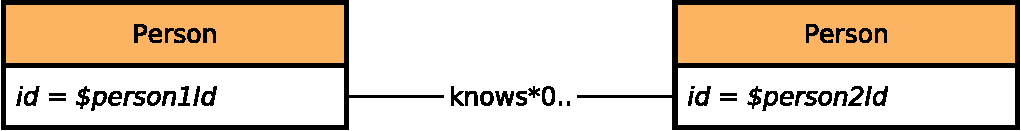
\includegraphics[scale=\patternscale,margin=0cm .2cm]{patterns/interactive-complex-read-13}} \\ \hline
%
	desc. & Given two Persons, find the shortest path between these two Persons in
the subgraph induced by the Knows relationships.

Return the length of this path:

\begin{itemize}
\tightlist
\item
  \(-1\) : no path found
\item
  \(0\): start person = end person
\item
  \(> 0\): regular case
\end{itemize}
 \\ \hline
%
	
		params &
		\innerCardVSpace{\begin{tabularx}{\attributeCardWidth}{|>{\paramNumberCell}c|>{\varNameCell}M|>{\typeCell}m{\typeWidth}|Y|} \hline
		$\mathsf{1}$ & person1.id
 & ID
 &  \\ \hline
		$\mathsf{2}$ & person2.id
 & ID
 &  \\ \hline
		\end{tabularx}}\innerCardVSpace \\ \hline
	
%
	
		result &
		\innerCardVSpace{\begin{tabularx}{\attributeCardWidth}{|>{\resultNumberCell}c|>{\varNameCell}M|>{\typeCell}m{\typeWidth}|>{\resultOriginCell}c|Y|} \hline
		$\mathsf{1}$ & length & 32-bit Integer & C &
				 \\ \hline
		\end{tabularx}}\innerCardVSpace \\ \hline
	
%
	%
	%
	CPs &
	\multicolumn{1}{>{\raggedright}l|}{
		\chokePoint{3.3}, 
		\chokePoint{7.2}, 
		\chokePoint{7.3}
		} \\ \hline
	%
	relevance &
		\small This query looks for a variable length path, starting at a given Person and finishing at an another given Person.
Proper cardinality estimation and search space prunning, will be crucial. This query also allows for possible parallel
implementations.
 \\ \hline%
\end{tabularx}
\queryCardVSpace

% change \emph back to the old one
\renewcommand{\emph}[1]{\oldemph{#1}}
\renewcommand*{\arraystretch}{1.1}

\noindent\begin{tabularx}{17cm}{|p{1.95cm}|X|}
	\hline
	workload    & Interactive / complex \\ \hline
%
	query       & 14 \\ \hline
%
	title       & Weighted/unweighted paths \\ \hline
%
    pattern     & \hfill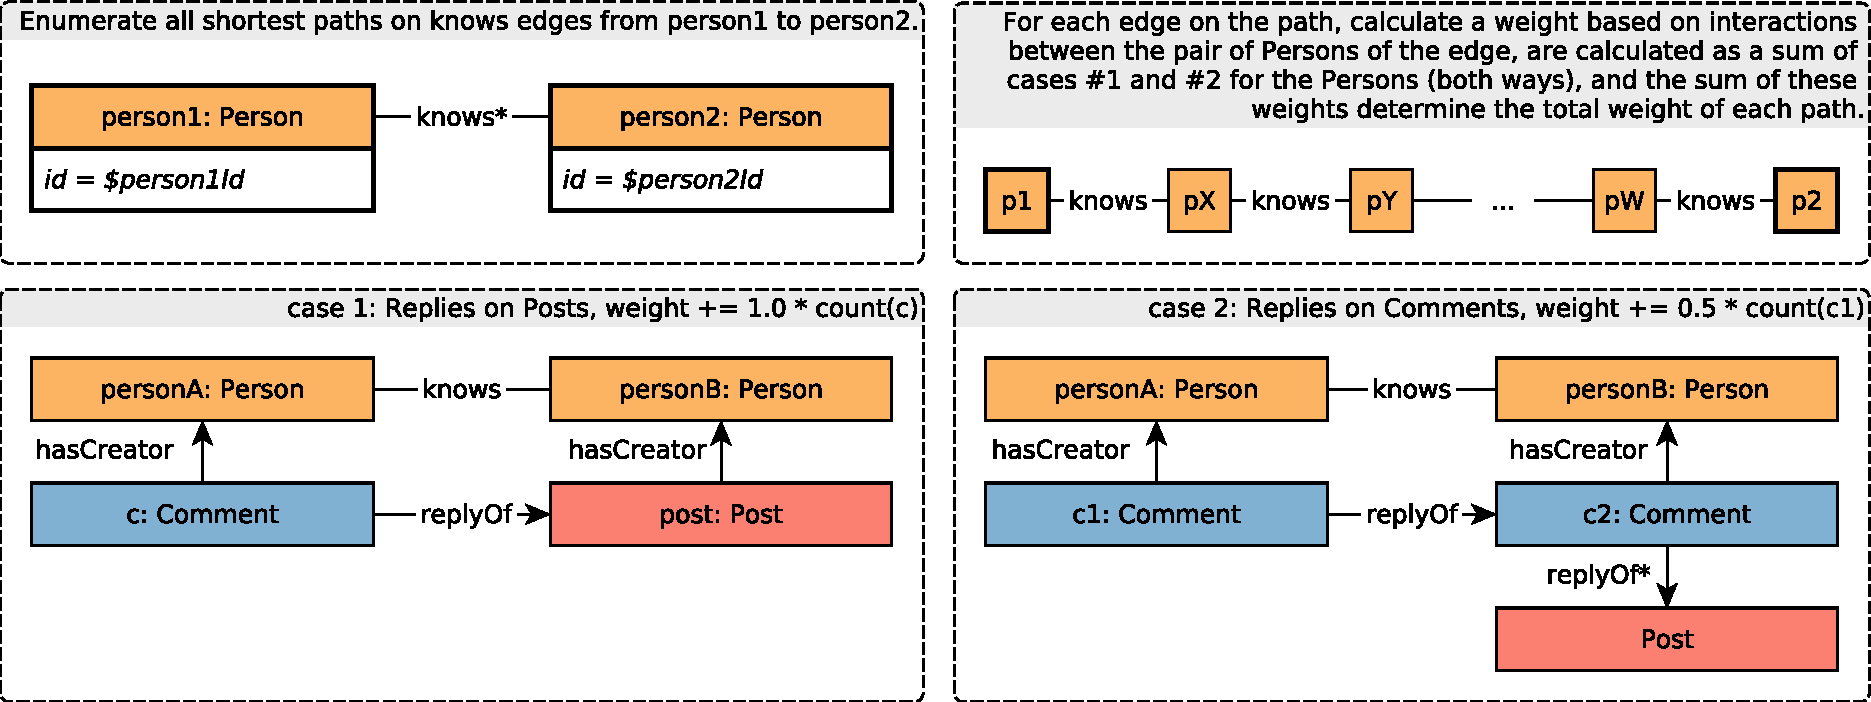
\includegraphics[scale=\patternscale,margin=0cm .2cm]{patterns/interactive-complex-read-14}\hfill\vadjust{} \\ \hline
%
	description & Given two Persons, find all (unweighted) shortest paths between these
two Persons, in the subgraph induced by the Knows relationship. Then,
for each path calculate a weight. The nodes in the path are Persons, and
the weight of a path is the sum of weights between every pair of
consecutive Person nodes in the path. The weight for a pair of Persons
is calculated such that every reply (by one of the Persons) to a Post
(by the other Person) contributes 1.0, and every reply (by ones of the
Persons) to a Comment (by the other Person) contributes 0.5. Return all
the paths with shortest length, and their weights.
 \\ \hline
%
	
%
	parameters  &
	\vspace{1.1ex}{\begin{tabularx}{14.2cm}{|c|M|m{2cm}|Y|} \hline
	\cellcolor{black!70} \color{white} $\mathsf{1}$ & \varname{person1.id} & \cellcolor{gray!20} \vartype{ID} &  \\ \hline
	\cellcolor{black!70} \color{white} $\mathsf{2}$ & \varname{person2.id} & \cellcolor{gray!20} \vartype{ID} &  \\ \hline
	\end{tabularx}}\vspace{1.1ex} \\ \hline
%
	
	result      &
	\vspace{1.1ex}{\begin{tabularx}{14.2cm}{|c|M|m{2cm}|Y|} \hline
	\cellcolor{black!70} \color{white} $\mathsf{1}$ & \varname{[Person.id]} & \cellcolor{gray!20} \vartype{[ID]} & Identifiers representing an ordered sequence of the Persons in the path \\ \hline
	\cellcolor{black!70} \color{white} $\mathsf{2}$ & \varname{weight} & \cellcolor{gray!20} \vartype{64-bit Float} &  \\ \hline
	\end{tabularx}}\vspace{1.1ex} \\ \hline
	
%
	sort        &
	\vspace{1.1ex}{\begin{tabular}{|c|l|c|} \hline
	\cellcolor{black!70} \color{white} $\mathsf{1}$ & \varname{weight} & \cellcolor{gray!20} $\desc$ \\ \hline
	\end{tabular}}\vspace{1.1ex} \\ \hline
	%
	%
	%
\end{tabularx}

\subsection{Short Reads Query Descriptions}

\todo{These could also be reworked as query cards.}
\renewcommand*{\arraystretch}{1.1}

\label{sec:interactive-short-read-01}
\noindent\begin{tabularx}{\queryCardWidth}{|>{\queryPropertyCell}c|X|}
	\hline
	query & Interactive / short / 1 \\ \hline
%
	title & Person Profile \\ \hline
%
    pattern & \hfill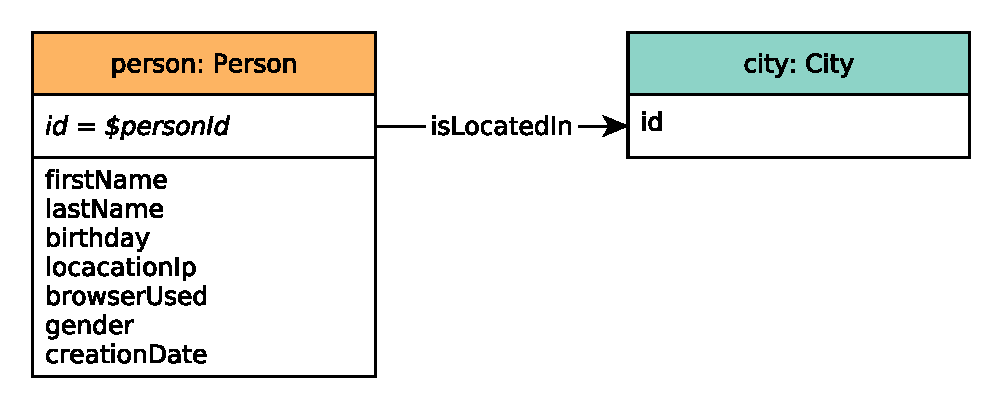
\includegraphics[scale=\patternscale,margin=0cm .2cm]{patterns/interactive-short-read-01}\hfill\vadjust{} \\ \hline
%
	desc. & Given a start Person, retrieve their first name, last name, birthday, IP
address, browser, and city of residence.
 \\ \hline
%
	
%
    
        params &
        \innerCardVSpace{\begin{tabularx}{\attributeCardWidth}{|>{\paramNumberCell}c|>{\varNameCell}M|>{\typeCell}m{\typeWidth}|Y|} \hline
        \cellcolor{parameter} \color{white} \footnotesize $\mathsf{1}$ &Person.id& ID &  \\ \hline
        \end{tabularx}}\innerCardVSpace \\ \hline
	
%
	
        result &
        \innerCardVSpace{\begin{tabularx}{\attributeCardWidth}{|>{\resultNumberCell}c|>{\varNameCell}M|>{\typeCell}m{\typeWidth}|>{\resultOriginCell}c|Y|} \hline
        $\mathsf{1}$ & Person.firstName & String &R&
                 \\ \hline
        $\mathsf{2}$ & Person.lastName & String &R&
                 \\ \hline
        $\mathsf{3}$ & Person.birthDay & Date &R&
                 \\ \hline
        $\mathsf{4}$ & Person.locationIP & String &R&
                 \\ \hline
        $\mathsf{5}$ & Person.browserUsed & String &R&
                 \\ \hline
        $\mathsf{6}$ & Person-isLocatedIn->Place.id & 32-bit Integer &R&
                 \\ \hline
        $\mathsf{7}$ & Person.gender & String &R&
                 \\ \hline
        $\mathsf{8}$ & Person.creationDate & DateTime &R&
                 \\ \hline
        \end{tabularx}}\innerCardVSpace \\ \hline
	
%
	%
	%
	%
    %
\end{tabularx}
\queryCardVSpace
\renewcommand*{\arraystretch}{1.1}

\noindent\begin{tabularx}{17cm}{|p{1.95cm}|X|}
	\hline
	workload    & Interactive / short \\ \hline
%
	query       & 2 \\ \hline
%
	title       & Person Recent Messages \\ \hline
%
    pattern     & \hfill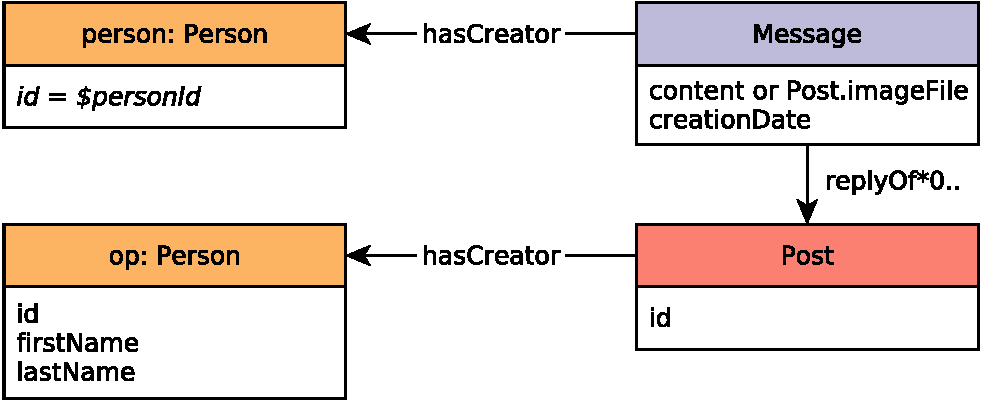
\includegraphics[scale=\patternscale,margin=0cm .2cm]{patterns/interactive-short-read-02}\hfill\vadjust{} \\ \hline
%
	description & Given a start Person, retrieve the last 10 Messages created by that
user. For each message, return that message, the original post in its
conversation, and the author of that post. If any of the Messages is a
Post, then the original Post will be the same Message, i.e.~that Message
will appear twice in that result.
 \\ \hline
%
	
%
	parameters  &
	\vspace{1.1ex}{\begin{tabularx}{14.2cm}{|c|M|m{2cm}|Y|} \hline
	\cellcolor{black!70} \color{white} $\mathsf{1}$ & \varname{Person.id} & \cellcolor{gray!20} \vartype{ID} &  \\ \hline
	\end{tabularx}}\vspace{1.1ex} \\ \hline
%
	
	result      &
	\vspace{1.1ex}{\begin{tabularx}{14.2cm}{|c|M|m{2cm}|Y|} \hline
	\cellcolor{black!70} \color{white} $\mathsf{1}$ & \varname{Message.id} & \cellcolor{gray!20} \vartype{64-bit Integer} &  \\ \hline
	\cellcolor{black!70} \color{white} $\mathsf{2}$ & \varname{Message.content or Post.imageFile} & \cellcolor{gray!20} \vartype{String} &  \\ \hline
	\cellcolor{black!70} \color{white} $\mathsf{3}$ & \varname{Message.creationDate} & \cellcolor{gray!20} \vartype{DateTime} &  \\ \hline
	\cellcolor{black!70} \color{white} $\mathsf{4}$ & \varname{Post.id or Comment-replyOf*->Post.id} & \cellcolor{gray!20} \vartype{ID} &  \\ \hline
	\cellcolor{black!70} \color{white} $\mathsf{5}$ & \varname{Post-hasCreator->Person.id or Comment-replyOf*->Post-hasCreator->Person.id} & \cellcolor{gray!20} \vartype{ID} &  \\ \hline
	\cellcolor{black!70} \color{white} $\mathsf{6}$ & \varname{Post-hasCreator->Person.firstName or Comment-replyOf*->Post-hasCreator->Person.firstName} & \cellcolor{gray!20} \vartype{String} &  \\ \hline
	\cellcolor{black!70} \color{white} $\mathsf{7}$ & \varname{Post-hasCreator->Person.lastName or Comment-replyOf*->Post-hasCreator->Person.lastName} & \cellcolor{gray!20} \vartype{String} &  \\ \hline
	\end{tabularx}}\vspace{1.1ex} \\ \hline
	
%
	sort        &
	\vspace{1.1ex}{\begin{tabular}{|c|l|c|} \hline
	\cellcolor{black!70} \color{white} $\mathsf{1}$ & \varname{Message.creationDate} & \cellcolor{gray!20} $\desc$ \\ \hline
	\cellcolor{black!70} \color{white} $\mathsf{2}$ & \varname{Message.id} & \cellcolor{gray!20} $\desc$ \\ \hline
	\end{tabular}}\vspace{1.1ex} \\ \hline
	%
	%
	%
\end{tabularx}
\vspace{2ex}
\renewcommand*{\arraystretch}{1.1}

\subsection*{Interactive / short / 3}
\label{section:interactive-short-read-03}

% change \emph{} to use sans-serif font
\let\oldemph\emph
\renewcommand{\emph}[1]{{\footnotesize \sf #1}}



\noindent\begin{tabularx}{\queryCardWidth}{|>{\queryPropertyCell}p{\queryPropertyCellWidth}|X|}
	\hline
	query & Interactive / short / 3 \\ \hline
%
	title & Person Friends \\ \hline
%
	pattern & \multicolumn{1}{c|}{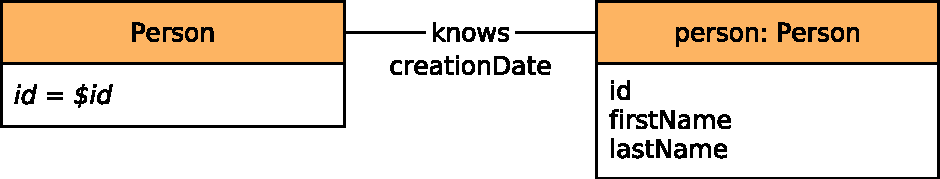
\includegraphics[scale=\patternscale,margin=0cm .2cm]{patterns/interactive-short-read-03}} \\ \hline
%
	desc. & Given a start Person, retrieve all of their friends, and the date at
which they became friends.
 \\ \hline
%
	
		params &
		\innerCardVSpace{\begin{tabularx}{\attributeCardWidth}{|>{\paramNumberCell}c|>{\varNameCell}M|>{\typeCell}m{\typeWidth}|Y|} \hline
		$\mathsf{1}$ & Person.id
 & ID
 &  \\ \hline
		\end{tabularx}}\innerCardVSpace \\ \hline
	
%
	
		result &
		\innerCardVSpace{\begin{tabularx}{\attributeCardWidth}{|>{\resultNumberCell}c|>{\varNameCell}M|>{\typeCell}m{\typeWidth}|>{\resultOriginCell}c|Y|} \hline
		$\mathsf{1}$ & Person.id & ID & R &
				 \\ \hline
		$\mathsf{2}$ & Person.firstName & String & R &
				 \\ \hline
		$\mathsf{3}$ & Person.lastName & String & R &
				 \\ \hline
		$\mathsf{4}$ & Knows.creationDate & DateTime & R &
				 \\ \hline
		\end{tabularx}}\innerCardVSpace \\ \hline
	
%
	
		sort		&
		\innerCardVSpace{\begin{tabularx}{\attributeCardWidth}{|>{\sortNumberCell}c|>{\varNameCell}M|>{\directionCell}c|Y|} \hline
		$\mathsf{1}$ & Knows.creationDate
 & $\desc
$ &  \\ \hline
		$\mathsf{2}$ & Person.id
 & $\asc
$ &  \\ \hline
		\end{tabularx}}\innerCardVSpace \\ \hline
	%
	%
	%
	%
\end{tabularx}
\queryCardVSpace

% change \emph back to the old one
\renewcommand{\emph}[1]{\oldemph{#1}}
\renewcommand*{\arraystretch}{1.1}

\subsection*{Interactive / short / 4}
\label{section:interactive-short-read-04}

% change \emph{} to use sans-serif font
\let\oldemph\emph
\renewcommand{\emph}[1]{{\footnotesize \sf #1}}



\noindent\begin{tabularx}{\queryCardWidth}{|>{\queryPropertyCell}p{\queryPropertyCellWidth}|X|}
	\hline
	query & Interactive / short / 4 \\ \hline
%
	title & Message Content \\ \hline
%
	pattern & \hfill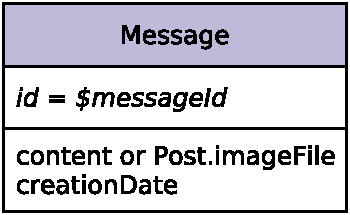
\includegraphics[scale=\patternscale,margin=0cm .2cm]{patterns/interactive-short-read-04}\hfill\vadjust{} \\ \hline
%
	desc. & Given a Message, retrieve its content and creation date.
 \\ \hline
%
	
		params &
		\innerCardVSpace{\begin{tabularx}{\attributeCardWidth}{|>{\paramNumberCell}c|>{\varNameCell}M|>{\typeCell}m{\typeWidth}|Y|} \hline
		$\mathsf{1}$ & Message.id
 & ID
 &  \\ \hline
		\end{tabularx}}\innerCardVSpace \\ \hline
	
%
	
		result &
		\innerCardVSpace{\begin{tabularx}{\attributeCardWidth}{|>{\resultNumberCell}c|>{\varNameCell}M|>{\typeCell}m{\typeWidth}|>{\resultOriginCell}c|Y|} \hline
		$\mathsf{1}$ & Message.creationDate & ID & R &
				 \\ \hline
		$\mathsf{2}$ & Message.content or Post.imageFile & String & R &
				 \\ \hline
		\end{tabularx}}\innerCardVSpace \\ \hline
	
%
	%
	%
	%
	%
\end{tabularx}
\queryCardVSpace

% change \emph back to the old one
\renewcommand{\emph}[1]{\oldemph{#1}}
\renewcommand*{\arraystretch}{1.1}

\noindent\begin{tabularx}{17cm}{|>{\small \sf}c|X|}
	\hline
	query    & Interactive / short / 5 \\ \hline
%
	title       & Message Creator \\ \hline
%
    pattern     & \hfill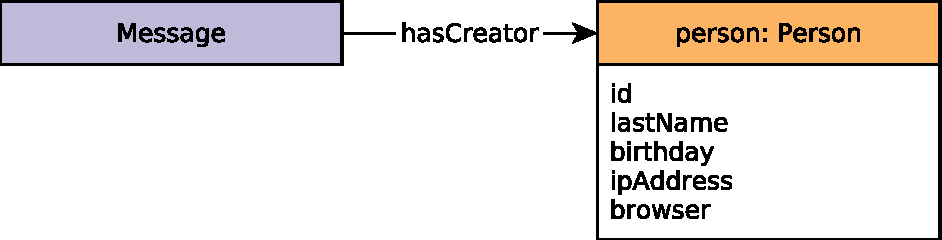
\includegraphics[scale=\patternscale,margin=0cm .2cm]{patterns/interactive-short-read-05}\hfill\vadjust{} \\ \hline
%
	desc. & Given a Message, retrieve its author.
 \\ \hline
%
	
%
	params.  &
	\vspace{1.1ex}{\begin{tabularx}{14.66cm}{|c|M|m{2cm}|Y|} \hline
	\cellcolor{parameter} \color{white} $\mathsf{1}$ & \varname{Message.id} & \cellcolor{gray!20} \vartype{ID} &  \\ \hline
	\end{tabularx}}\vspace{1.1ex} \\ \hline
%
	
	result      &
	\vspace{1.1ex}{\begin{tabularx}{14.66cm}{|c|M|m{2cm}|c|Y|} \hline
	\cellcolor{result} \color{white} $\mathsf{1}$ & \varname{Message-hasCreator->Person.id} & \cellcolor{gray!20} \vartype{ID} &
	    \texttt{R} &
	     \\ \hline
	\cellcolor{result} \color{white} $\mathsf{2}$ & \varname{Message-hasCreator->Person.firstName} & \cellcolor{gray!20} \vartype{String} &
	    \texttt{R} &
	     \\ \hline
	\cellcolor{result} \color{white} $\mathsf{3}$ & \varname{Message-hasCreator->Person.lastName} & \cellcolor{gray!20} \vartype{String} &
	    \texttt{R} &
	     \\ \hline
	\end{tabularx}}\vspace{1.1ex} \\ \hline
	
%
	%
	%
	%
    %
\end{tabularx}
\vspace{2ex}
\renewcommand*{\arraystretch}{1.1}

\subsection*{Interactive / short / 6}
\label{sec:interactive-short-read-06}

\noindent\begin{tabularx}{\queryCardWidth}{|>{\queryPropertyCell}c|X|}
	\hline
	query & Interactive / short / 6 \\ \hline
%
	title & Message Forum \\ \hline
%
    pattern & \hfill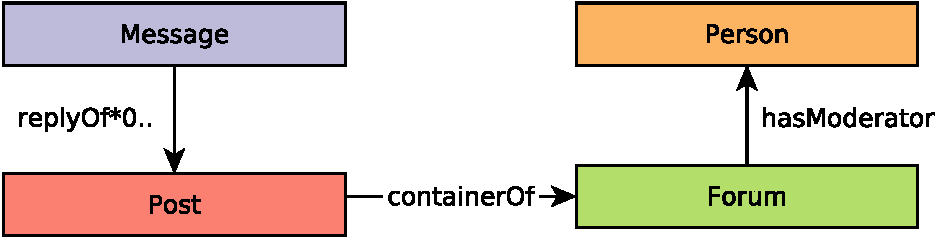
\includegraphics[scale=\patternscale,margin=0cm .2cm]{patterns/interactive-short-read-06}\hfill\vadjust{} \\ \hline
%
	desc. & Given a Message, retrieve the Forum that contains it and the Person that
moderates that forum. Since comments are not directly contained in
forums, for comments, return the forum containing the original post in
the thread which the comment is replying to.
 \\ \hline
%
	
%
    
        params &
        \innerCardVSpace{\begin{tabularx}{\attributeCardWidth}{|>{\paramNumberCell}c|>{\varNameCell}M|>{\typeCell}m{\typeWidth}|Y|} \hline
        \cellcolor{parameter} \color{white} \footnotesize $\mathsf{1}$ &Message.id& ID &  \\ \hline
        \end{tabularx}}\innerCardVSpace \\ \hline
	
%
	
        result &
        \innerCardVSpace{\begin{tabularx}{\attributeCardWidth}{|>{\resultNumberCell}c|>{\varNameCell}M|>{\typeCell}m{\typeWidth}|>{\resultOriginCell}c|Y|} \hline
        $\mathsf{1}$ & Message<-containerOf-Forum.id & ID &R&
                 \\ \hline
        $\mathsf{2}$ & Message<-containerOf-Forum.title & String &R&
                 \\ \hline
        $\mathsf{3}$ & Message<-containerOf-Forum-hasModerator->Person.id & ID &R&
                 \\ \hline
        $\mathsf{4}$ & Message<-containerOf-Forum-hasModerator->Person.firstName & String &R&
                 \\ \hline
        $\mathsf{5}$ & Message<-containerOf-Forum-hasModerator->Person.lastName & String &R&
                 \\ \hline
        \end{tabularx}}\innerCardVSpace \\ \hline
	
%
	%
	%
	%
    %
\end{tabularx}
\queryCardVSpace
\renewcommand*{\arraystretch}{1.1}

\subsection*{Interactive / short / 7}
\label{section:interactive-short-read-07}

% change \emph{} to use sans-serif font
\let\oldemph\emph
\renewcommand{\emph}[1]{{\footnotesize \sf #1}}



\noindent\begin{tabularx}{\queryCardWidth}{|>{\queryPropertyCell}p{\queryPropertyCellWidth}|X|}
	\hline
	query & Interactive / short / 7 \\ \hline
%
	title & Message Replies
 \\ \hline
%
	pattern & \hfill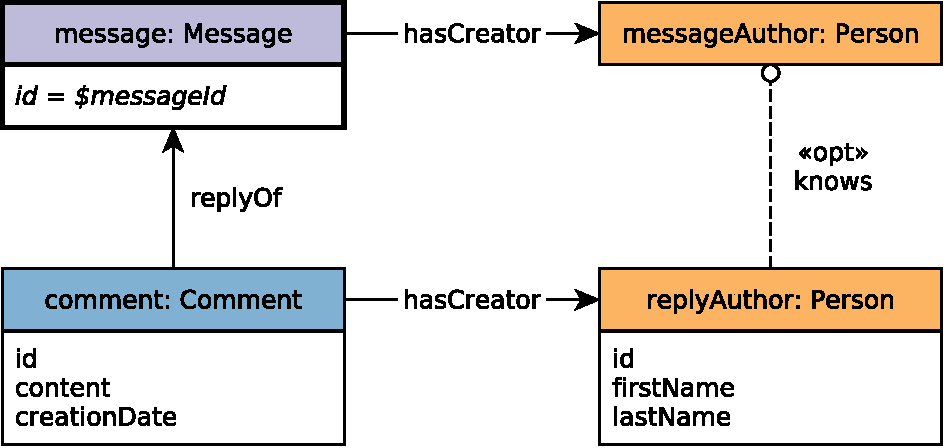
\includegraphics[scale=\patternscale,margin=0cm .2cm]{patterns/interactive-short-read-07}\hfill\vadjust{} \\ \hline
%
	desc. & Given a Message, retrieve the (1-hop) Comments that reply to it.

In addition, return a boolean flag \texttt{knows} indicating if the
author of the reply knows the author of the original message. If author
is same as original author, return false for \texttt{knows} flag.
 \\ \hline
%
	
		params &
		\innerCardVSpace{\begin{tabularx}{\attributeCardWidth}{|>{\paramNumberCell}c|>{\varNameCell}M|>{\typeCell}m{\typeWidth}|Y|} \hline
		$\mathsf{1}$ & Message.id
 & ID
 &  \\ \hline
		\end{tabularx}}\innerCardVSpace \\ \hline
	
%
	
		result &
		\innerCardVSpace{\begin{tabularx}{\attributeCardWidth}{|>{\resultNumberCell}c|>{\varNameCell}M|>{\typeCell}m{\typeWidth}|>{\resultOriginCell}c|Y|} \hline
		$\mathsf{1}$ & Message\textless{}-replyOf-Comment.id & ID & R &
				 \\ \hline
		$\mathsf{2}$ & Message\textless{}-replyOf-Comment.content & String & R &
				 \\ \hline
		$\mathsf{3}$ & Message\textless{}-replyOf-Comment.creationDate & DateTime & R &
				 \\ \hline
		$\mathsf{4}$ & Comment-hasCreator-\textgreater{}Person.id & ID & R &
				 \\ \hline
		$\mathsf{5}$ & Comment-hasCreator-\textgreater{}Person.firstName & String & R &
				 \\ \hline
		$\mathsf{6}$ & Comment-hasCreator-\textgreater{}Person.lastName & String & R &
				 \\ \hline
		$\mathsf{7}$ & knows & Boolean & C &
				Original message author knows reply author
 \\ \hline
		\end{tabularx}}\innerCardVSpace \\ \hline
	
%
	
		sort		&
		\innerCardVSpace{\begin{tabularx}{\attributeCardWidth}{|>{\sortNumberCell}c|>{\varNameCell}M|>{\directionCell}c|Y|} \hline
		$\mathsf{1}$ & Message\textless{}-replyOf-Comment.creationDate
 & $\desc
$ &  \\ \hline
		$\mathsf{2}$ & Message-hasCreator-\textgreater{}Person.id
 & $\asc
$ &  \\ \hline
		\end{tabularx}}\innerCardVSpace \\ \hline
	%
	%
	%
	%
\end{tabularx}
\queryCardVSpace

% change \emph back to the old one
\renewcommand{\emph}[1]{\oldemph{#1}}


%\renewcommand*{\arraystretch}{1.1}

\label{sec:interactive-short-read-01}
\noindent\begin{tabularx}{\queryCardWidth}{|>{\queryPropertyCell}c|X|}
	\hline
	query & Interactive / short / 1 \\ \hline
%
	title & Person Profile \\ \hline
%
    pattern & \hfill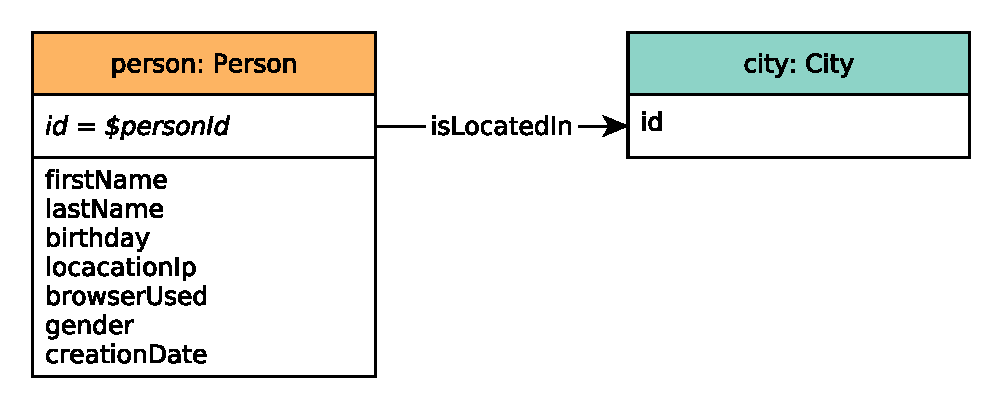
\includegraphics[scale=\patternscale,margin=0cm .2cm]{patterns/interactive-short-read-01}\hfill\vadjust{} \\ \hline
%
	desc. & Given a start Person, retrieve their first name, last name, birthday, IP
address, browser, and city of residence.
 \\ \hline
%
	
%
    
        params &
        \innerCardVSpace{\begin{tabularx}{\attributeCardWidth}{|>{\paramNumberCell}c|>{\varNameCell}M|>{\typeCell}m{\typeWidth}|Y|} \hline
        \cellcolor{parameter} \color{white} \footnotesize $\mathsf{1}$ &Person.id& ID &  \\ \hline
        \end{tabularx}}\innerCardVSpace \\ \hline
	
%
	
        result &
        \innerCardVSpace{\begin{tabularx}{\attributeCardWidth}{|>{\resultNumberCell}c|>{\varNameCell}M|>{\typeCell}m{\typeWidth}|>{\resultOriginCell}c|Y|} \hline
        $\mathsf{1}$ & Person.firstName & String &R&
                 \\ \hline
        $\mathsf{2}$ & Person.lastName & String &R&
                 \\ \hline
        $\mathsf{3}$ & Person.birthDay & Date &R&
                 \\ \hline
        $\mathsf{4}$ & Person.locationIP & String &R&
                 \\ \hline
        $\mathsf{5}$ & Person.browserUsed & String &R&
                 \\ \hline
        $\mathsf{6}$ & Person-isLocatedIn->Place.id & 32-bit Integer &R&
                 \\ \hline
        $\mathsf{7}$ & Person.gender & String &R&
                 \\ \hline
        $\mathsf{8}$ & Person.creationDate & DateTime &R&
                 \\ \hline
        \end{tabularx}}\innerCardVSpace \\ \hline
	
%
	%
	%
	%
    %
\end{tabularx}
\queryCardVSpace

\subsection{Update Query Descriptions}

\todo{Maybe introduce YAML specification for these as well?}
{\small
\begin{enumerate}
    \item Add Person
        \begin{itemize}
            \item \textbf{Description:} Add a Person to the social network.
            \item \textbf{Parameters:} \\
                \begin{tabular}{lll}
                    Person.id 	 			& ID & \parbox[t]{20cm}{\par \strut} \\
                    Person.firstName 		& String & \parbox[t]{20cm}{\par \strut} \\
                    Person.lastName 		& String & \parbox[t]{20cm}{\par \strut} \\
                    Person.gender 		& String & \parbox[t]{20cm}{\par \strut} \\
                    Person.birthDay 		& Date & \parbox[t]{20cm}{\par \strut} \\
                    Person.creationDate     & DateTime & \parbox[t]{20cm}{\par \strut} \\
                    Person.locationIp     & String & \parbox[t]{20cm}{\par \strut} \\
                    Person.browserUsed     & String & \parbox[t]{20cm}{\par \strut} \\
                    Person-isLocatedIn->City.id 	& ID & \parbox[t]{20cm}{\par \strut} \\
                    Person.speaks 	& \{ String \} & \parbox[t]{20cm}{\par \strut} \\
                    Person.emails 	& \{ String \} & \parbox[t]{20cm}{\par \strut} \\
                    Person-hasInterest->Tag.id 	& \{ ID \} & \parbox[t]{20cm}{\par \strut} \\
                    \{ Person-studyAt->University.id, \\
                    Person-studyAt->.classYear \}  & \{ID, 32-bit Integer\} & \parbox[t]{20cm}{\par \strut} \\
                        \{ Person-workAt->Company.id, \\
                        Person-workAt->.workFrom \}  & \{ID, 32-bit Integer\} & \parbox[t]{20cm}{\par \strut} \\
                        \end{tabular}
                \end{itemize}
            \item Add Post Like
                \begin{itemize}
                    \item \textbf{Description:} Add a Like to a Post of the social network.
                    \item \textbf{Parameters:} \\
                        \begin{tabular}{lll}
                            Person.id 	 			& ID & \parbox[t]{20cm}{\par \strut} \\
                            Post.id 	 			& ID & \parbox[t]{20cm}{\par \strut} \\
                            Person-likes->.creationDate 	 		& DateTime & \parbox[t]{20cm}{\par \strut} \\
                        \end{tabular}
                \end{itemize}
            \item Add Comment Like
                \begin{itemize}
                    \item \textbf{Description: Add a Like to a Comment of the social network.}
                    \item \textbf{Parameters:} \\
                        \begin{tabular}{lll}
                            Person.id 	 			& ID & \parbox[t]{20cm}{\par \strut} \\
                            Comment.id 	 			& ID & \parbox[t]{20cm}{\par \strut} \\
                            Person-likes->.creationDate 	 		& DateTime & \parbox[t]{20cm}{\par \strut} \\
                        \end{tabular}
                \end{itemize}
            \item Add Forum
                \begin{itemize}
                    \item \textbf{Description:} Add a Forum to the social network.
                    \item \textbf{Parameters:} \\
                        \begin{tabular}{lll}
                            Forum.id 	 			& ID & \parbox[t]{20cm}{// person 1\strut} \\
                            Forum.title 	 			& String & \parbox[t]{20cm}{// person 2\strut} \\
                            Forum.creationDate & DateTime & \parbox[t]{20cm}{\par \strut} \\
                            Forum-hasModerator->Person.id 	& \{ ID \} & \parbox[t]{20cm}{\par \strut} \\
                            Forum-hasTag->Tag.id 	& \{ ID \} & \parbox[t]{20cm}{\par \strut} \\
                        \end{tabular}
                \end{itemize}
            \item Add Forum Membership
                \begin{itemize}
                    \item \textbf{Description:} Add a Forum membership to the social network.
                    \item \textbf{Parameters:} \\
                        \begin{tabular}{lll}
                            Person.id 	 			& ID & \parbox[t]{20cm}{\par \strut} \\
                            Person-hasMember->Forum.id 	 			& ID & \parbox[t]{20cm}{\par \strut} \\
                            Person-hasMember->.joinDate 	 		& DateTime & \parbox[t]{20cm}{\par \strut} \\
                        \end{tabular}
                \end{itemize}
            \item Add Post
                \begin{itemize}
                    \item \textbf{Description:} Add a Post to the social network.
                    \item \textbf{Parameters:} \\
                        \begin{tabular}{lll}
                            Post.id 	 			& ID & \parbox[t]{20cm}{\par \strut} \\
                            Post.imageFile 	 			& String & \parbox[t]{20cm}{\par \strut} \\
                            Post.creationDate 	 		& DateTime & \parbox[t]{20cm}{\par \strut} \\
                            Post.locationIp 	 		& String & \parbox[t]{20cm}{\par \strut} \\
                            Post.browserUsed 	 		& String & \parbox[t]{20cm}{\par \strut} \\
                            Post.language 	 		    & String & \parbox[t]{20cm}{\par \strut} \\
                            Post.content 	 		    & Text & \parbox[t]{20cm}{\par \strut} \\
                            Post.length 	 		    & 32-bit Integer & \parbox[t]{20cm}{\par \strut} \\
                            Post-hasCreator->Person.id & ID & \parbox[t]{20cm}{\par \strut} \\
                            Forum-containerOf->Post.id & ID & \parbox[t]{20cm}{\par \strut} \\
                            Post-isLocatedIn->Country.id & ID & \parbox[t]{20cm}{\par \strut} \\
                            \{Post-hasTag->Tag.id\} & \{ID\} & \parbox[t]{20cm}{\par \strut} \\
                        \end{tabular}
                \end{itemize}
            \item Add Comment
                \begin{itemize}
                    \item \textbf{Description:} Add a Comment replying to a Post/Comment to the social network.
                    \item \textbf{Parameters:} \\
                        \begin{tabular}{lll}
                            Comment.id 	 			& ID & \parbox[t]{20cm}{\par \strut} \\
                            Comment.creationDate 			& DateTime & \parbox[t]{20cm}{\par \strut} \\
                            Comment.locationIp 	 		& String & \parbox[t]{20cm}{\par \strut} \\
                            Comment.browserUsed 	 		& String & \parbox[t]{20cm}{\par \strut} \\
                            Comment.content 	 		    & Text & \parbox[t]{20cm}{\par \strut} \\
                            Comment.length 	 		    & 32-bit Integer & \parbox[t]{20cm}{\par \strut} \\
                            Comment-hasCreator->Person.id & ID & \parbox[t]{20cm}{\par \strut} \\
                            Comment-isLocatedIn->Country.id & ID & \parbox[t]{20cm}{\par \strut} \\
                            Comment-replyOf->Post.id & ID & \parbox[t]{20cm}{ // -1 if the comment is a reply of a comment. \strut} \\
                            Comment-replyOf->Comment.id & ID & \parbox[t]{20cm}{// -1 if the comment is a reply of a post. \strut} \\
                            \{Comment-hasTag->Tag.id\} & \{ID\} & \parbox[t]{20cm}{\par \strut} \\
                        \end{tabular}
                \end{itemize}
            \item Add Friendship
                \begin{itemize}
                    \item \textbf{Description:} Add a friendship relation to the social network
                    \item \textbf{Parameters:} \\
                        \begin{tabular}{lll}
                            Person.id 	 			& ID & \parbox[t]{20cm}{// person 1\strut} \\
                            Person.id 	 			& ID & \parbox[t]{20cm}{// person 2\strut} \\
                            Person-knows->.creationDate & DateTime & \parbox[t]{20cm}{\par \strut} \\
                        \end{tabular}
                \end{itemize}
        \end{enumerate}
      }


\section{Substitution Parameters}

\input{interactive-parameters}

\section{Load Definition}


\input{interactive-workload}


\subsection{Business Intelligence Workload}
\subsubsection{Choke Points}

\subsubsection{Business Intelligence Queries}

{\small
    \begin{enumerate}
      \item Posting summary 
            \begin{itemize}
                \item \textbf{Description:}
                  Given a date, find all Messages (Posts and Comments) created before than that date.
                  Group them by a three level grouping.

                  \begin{itemize}
                    \item First: by their year of creation.
                    \item Second: for each year, group them into Posts and Comments.
                    \item Third: for each year-type (Post or Comment) group, split it into four groups based on the
                              length of their content: 
                              \begin{itemize}
                                \item if length is less than 40, it is 'short'; 
                                \item else, if length is less than 80, it is 'one liner';
                                \item else, if length is less than 160, it is 'tweet';
                                \item otherwise, it is 'long'
                              \end{itemize}
                  \end{itemize}

                \item \textbf{Parameters:} \\
                    \begin{tabular}{ll}
                      date 										& DateTime \\
                    \end{tabular}
                \item \textbf{Results:} \\
                  For every third-level group, return the the following aggregates:
                    \begin{tabular}{lll}
                      year 					& 32-bit Integer & \\
                      Message.type	& String & \parbox[t]{20cm}{// "Post" or "Comment"  \strut} \\
                      Message.length & 32-bit Integer & \\
                      category & 32-bit Integer & \parbox[t]{20cm}{// 0 (short), 1 (one-liner), 2 (tweet), 3 (long) \strut}  \\
                      count & 32-bit Integer &  \parbox[t]{20cm}{// The number of messages in this group  \strut} \\
                      average & 32-bit Integer &  \parbox[t]{20cm}{// The average Message length \strut} \\
                      sum & 32-bit Integer &  \parbox[t]{20cm}{// The sum of the Messages lengths \strut} \\
                      percentage & 32-bit Floating Point &  \parbox[t]{20cm}{// The percentage of Messages in this group
                        out of the total number \par of Messages created before the given date  \strut} \\
                      \end{tabular}
                    Sort the results first by Year (descending), then by the Message.type (Post 1st, or Comment 2nd) and
                    finally by the category (ascending)
                    \end{itemize}

      \item Top Tags from Country, age, gender and time 
            \begin{itemize}
                \item \textbf{Description:}
                  Select all Messages created between date1 and date2 (both included) by Persons located in any country
                  of a provided list of countries Select the creators (Persons) and the Tags of these Messages .  Split
                  these persons, tags and Messages into a five level grouping:
                  \begin{itemize}
                    \item First by the name of the country of the Person
                    \item  Second, by the month when the Message was created
                    \item Third, by the gender of the person
                    \item      Four, by the age group of the Person, which is defined as:
                      \begin{itemize}
                        \item The difference in years between the Person's birthday and the end of
                          simulation ('2013-01-01'), divided by 5, rounded down.
                      \end{itemize}
                    \item  Fifth, by the name of the tag attached to the Message
                  \end{itemize}
                \item \textbf{Parameters:} \\
                    \begin{tabular}{ll}
                      date1 & Date \\
                      date2 & Date \\
                      list of country names & \{String\} \\
                      endDate & Date \\
                    \end{tabular}
                \item \textbf{Results:} \\
                  For each of the fifth-level groups return: 
                    \begin{tabular}{lll}
                      Country.name & String & \\
                      month & 32-bit Integer & \\
                      gender & String & \parbox[t]{20cm}{// "Male" or "Female" \strut}\\
                      age group & 32-bit Integer & \\
                      Tag.name & String & \\
                      count & 32-bit Integer & \parbox[t]{20cm}{// The count of Messages falling in this group \strut}
                    \end{tabular}
                    Return top 100 groups where number of Messages is bigger than 100. Sort the groups by the count
                    (descending), Tag name (ascending), age group (ascending), gender (ascending), month
                    (ascending) and country name (ascending).
                    \end{itemize}
      \item Tag Evolution 
            \begin{itemize}
                \item \textbf{Description:}
                  Given two date intervals (left-closed, right-open), for each of these intervals find all Tags that
                  were used in Messages. For each interval, count the number of Messages containing each Tag.

                \item \textbf{Parameters:} \\
                    \begin{tabular}{ll}
                      dateStart1 & Date \\
                      dateEnd1 & Date \\
                      dateStart2 & Date \\
                      dateEnd2 & Date \\
                    \end{tabular}
                \item \textbf{Results:} \\
                  For each of the tags:
                    \begin{tabular}{lll}
                      Tag.name & String & \\
                      countInterval1 & 32-bit Integer & \parbox[t]{20cm}{// The number of occurrences of this Tag during
                        interval 1  \strut} \\
                      countInterval2 & 32-bit Integer & \parbox[t]{20cm}{// The number of occurrences of this Tag during
                        interval 2 \strut}\\
                      diff & 32-bit Integer & \parbox[t]{20cm}{ // The absolute difference countInterval1 and
                        countInterval2 \strut} \\
                    \end{tabular}
                    Return top-100 results sorted by the difference (descending) and then the tag name (ascending)
                    \end{itemize}

      \item Popular topics in a Country 
            \begin{itemize}
                \item \textbf{Description:}
                  Given a tagCalss and a Country, find all the Forums created in the given Country, containing at least
                  one Posts with Tags belonging directly to the given tagClass.
                  The location of a Forum is identified by the location of the Forum’s moderator.
                \item \textbf{Parameters:} \\
                    \begin{tabular}{ll}
                      TagClass.name & String \\
                      Country.name & String \\
                    \end{tabular}
                \item \textbf{Results:} \\
                  For each Forum:
                    \begin{tabular}{lll}
                      Forum.id  & ID & \\
                      Forum.title & String & \\
                      Forum.creationDate & DateTime & \\
                      Forum-hasModerator->Person.id & \{ ID \} & \\
                      count & 32-bit Integer &  \parbox[t]{20cm}{ // The number of Posts in the Forum with at least \par one Tag belonging to
                        the TagClass \strut} 
                    \end{tabular}
                    Return top-20 results sorted by count (descending) and Forum.id (ascending)
                    \end{itemize}

      \item Top posters in a Country 
            \begin{itemize}
                \item \textbf{Description:}
                  Find the most popular Forums for a given Country, where the popularity of a Forum is measured by the
                  number of members that Forum has from the given Country.  If multiple forums have the same member
                  count, use forum ID as tie breaker for popularity, where lower ID is more popular.  For each person
                  that is a member or moderator of any of the 100 most popular Forums, count the number of Posts they
                  made in any of those (most popular) Forums.

                  Group persons by:
                  \begin{itemize}
                      \item First, id
                      \item Second, first name
                      \item Third, last name
                      \item Fourth, creation date
                  \end{itemize}
                \item \textbf{Parameters:} \\
                    \begin{tabular}{ll}
                      Country.name & String \\ 
                    \end{tabular}
                \item \textbf{Results:} \\
                   For each group:
                    \begin{tabular}{lll}
                      Person.id & ID & \\
                      Person.firstName & String & \\
                      Person.lastName & String & \\
                      Person.creationDate & DateTime & \\
                      count & 32-bit Integer & \parbox[t]{20cm}{ // Number of Posts created by that Person \par in the top-100
                        most popular Forums\strut}  \\
                    \end{tabular}
                    Return top 100 Persons, sorted by count (descending) and by Person.Id (ascending).
                    \end{itemize}

      \item Most active posters on a given topic 
            \begin{itemize}
                \item \textbf{Description:}
                  Retrieve Persons who have created a Message with given Tag.  For each Person, compute a score as
                  follows: (the number of Messages they created that have given Tag) PLUS (2 x number of replies to
                  those Messages) PLUS (10 x number of Likes on those Messages).
                \item \textbf{Parameters:} \\
                    \begin{tabular}{ll}
                      Tag.name & 32-bit Integer 
                    \end{tabular}
                \item \textbf{Results:} \\
                  For each Person:
                    \begin{tabular}{lll}
                      Person.id & ID & \\
                      replyCount & 32-bit Integer & \parbox[t]{20cm}{ //The number of replies to Messages with
                        the \par given Tag created by the Person \strut}  \\
                      likeCount & 32-bit Integer & \parbox[t]{20cm}{ //The number of likes to Messages with
                        the \par given Tag created by the Person \strut}  \\ 
                      messageCount & 32-bit Integer & \parbox[t]{20cm}{ //The number of Messages with
                        the \par given Tag created by the Person \strut}  \\
                      score & 32-bit Integer & \\
                    \end{tabular}
                    Return the top-100 Persons, sorted by score (descending) and Person.id (ascending)
                    \end{itemize}

      \item Most authorative Person on a given topic 
            \begin{itemize}
                \item \textbf{Description:}
                  Given a Tag, find all Persons that ever created a Message with the given Tag.
                  For each of these Persons compute their "authority score".
                  The "authority score" for a given Person is defined as the sum of "popularity scores" of the Persons
                  that liked any of that Person's Messages with the given Tag.
                  A Person's "popularity score" is defined as the total number of likes on all of their Messages.
                \item \textbf{Parameters:} \\
                    \begin{tabular}{ll}
                      Tag.name & String \\
                    \end{tabular}
                \item \textbf{Results:} \\

                  For each Person:

                    \begin{tabular}{lll}
                      Person.Id & ID & \\
                      authorityScore & 32-bit Integer & \\
                    \end{tabular}

                    Return the top 100 Persons sorted the authorityScore (descending) and Person.Id (ascending).
                    \end{itemize}

      \item Related Topics 
            \begin{itemize}
                \item \textbf{Description:}
                  Find all Messages that have a given Tag.    
                  Find the Tags attached to replies of these Messages, but only those replies that do not have the given
                  Tag. Group the Tags by name, and get the count of replies in each group.
                \item \textbf{Parameters:} \\
                    \begin{tabular}{ll}
                      Tag.name & String \\
                    \end{tabular}
                \item \textbf{Results:} \\
                  For each group:
                    \begin{tabular}{lll}
                      Tag.name & String & \\
                      count & 32-bit Integer & \parbox[t]{20cm}{ // The count of replies with the Tag \strut} \\
                    \end{tabular}
                    Return the top-100 Tags, sorted by count (descending) and by Tag.name (ascending).
                    \end{itemize}

      \item Forum with related Tags 
            \begin{itemize}
                \item \textbf{Description:}
                  Given two tagClasses, find those forums that contain Posts with Tags belonging tagClass1 and contain
                  Posts with Tags belonging to tagCalss2 (not transitive). Consider the forums with a number of members
                  greater than a given threshold.
                  For every such forum, count the number of Posts  that have a Tag from tagclass t1 (count1), and the
                  number of posts that have a tag  from the tagclass2. 
                \item \textbf{Parameters:} \\
                    \begin{tabular}{ll}
                      TagClass1.name & String \\ 
                      TagClass2.name & String \\ 
                      threshold & 32-bit Integer \\
                    \end{tabular}
                \item \textbf{Results:} \\
                  For each Forum:
                    \begin{tabular}{lll}
                      Forum.id & ID & \\
                      count1 & 32-bit Integer & \parbox[t]{20cm}{ // The count of Posts with at least one Tag belonging
                        to TagClass1 \strut} \\
                      count2 & 32-bit Integer & \parbox[t]{20cm}{ // The count of Posts with at least one Tag belonging
                        to TagClass2 \strut} \\
                    \end{tabular}
                    \end{itemize}

      \item Central Person for a topic 
            \begin{itemize}
                \item \textbf{Description:}
                  Given a Tag, find all Persons that are either interested on the Tag, or have written a Post with the
                  given Tag. For each Person, compute the score as the sum of the following two aspects:

                  \begin{itemize}
                    \item 100, if the Person has this tag as their interest, or 0 otherwise
                    \item number of posts by this person with the given tag
                  \end{itemize}

                \item \textbf{Parameters:} \\
                    \begin{tabular}{ll}
                      Tag.name & String \\
                    \end{tabular}
                \item \textbf{Results:} \\
                  For each Person:

                    \begin{tabular}{lll}
                      Person.Id & ID & \\
                      score & 32-bit Integer & \\
                      friendsScore & 32-bit Integer & \parbox[t]{20cm}{ // The sum of the score of the Person's friends\strut} \\
                    \end{tabular}

                    Return the top-100 Persons, sorted the sum of score and friendsScore (descending), and  Person.id
                    (ascending) 
                \end{itemize}

      \item Tag Evolution 
            \begin{itemize}
                \item \textbf{Description:}
                \item \textbf{Parameters:} \\
                    \begin{tabular}{ll}
                    \end{tabular}
                \item \textbf{Results:} \\
                    \begin{tabular}{lll}
                    \end{tabular}
                    \end{itemize}
\end{enumerate}
}


\chapter{Auditing Policies}
\label{sec:auditing}

\emph{This chapter contains the auditing policies for the LDBC Social Network Benchmark. The initial draft of the auiting policies were published in the EU project deliverable D6.3.3 ``LDBC Benchmark Auditing Policies''.}

%%%%%%%%%%%%%%%%%%%%%%%%%%%%%%%%%%%%%%%%%%%%%%%%%%%%%%%%%%%%%%%%%%%%%%%%%%%%%%
%%%%%%%%%%%%%%%%%%%%%%%%%%%%%%%%%%%%%%%%%%%%%%%%%%%%%%%%%%%%%%%%%%%%%%%%%%%%%%
%%%%%%%%%%%%%%%%%%%%%%%%%%%%%%%%%%%%%%%%%%%%%%%%%%%%%%%%%%%%%%%%%%%%%%%%%%%%%%

This chapter is divided in the following parts:
\begin{itemize}
    \item Motivation of benchmark result auditing
    \item General discussion of auditable aspects of benchmarks
    \item Specific checklists and running rules for the Social Network Benchmark's workloads (Interactive, Business Intelligence)
\end{itemize}

Many definitions and general considerations are shared between the benchmarks, hence it is justified to present the principles first and to refer to these in the context of the benchmark specific rules.

The auditing process, including the auditor certification exams, the possibility of challenging audited results, \etc, are defined in the LDBC Byelaws~\cite{ldbc_byelaws}. Please refer to the latest Byelaws document when conducting audits.

%%%%%%%%%%%%%%%%%%%%%%%%%%%%%%%%%%%%%%%%%%%%%%%%%%%%%%%%%%%%%%%%%%%%%%%%%%%%%%
%%%%%%%%%%%%%%%%%%%%%%%%%%%%%%%%%%%%%%%%%%%%%%%%%%%%%%%%%%%%%%%%%%%%%%%%%%%%%%
%%%%%%%%%%%%%%%%%%%%%%%%%%%%%%%%%%%%%%%%%%%%%%%%%%%%%%%%%%%%%%%%%%%%%%%%%%%%%%

\section{Rationale and General Principles}

%%%%%%%%%%%%%%%%%%%%%%%%%%%%%%%%%%%%%%%%%%%%%%%%%%%%%%%%%%%%%%%%%%%%%%%%%%%%%%
%%%%%%%%%%%%%%%%%%%%%%%%%%%%%%%%%%%%%%%%%%%%%%%%%%%%%%%%%%%%%%%%%%%%%%%%%%%%%%
%%%%%%%%%%%%%%%%%%%%%%%%%%%%%%%%%%%%%%%%%%%%%%%%%%%%%%%%%%%%%%%%%%%%%%%%%%%%%%

The purpose of benchmark auditing is to improve the \emph{credibility} and \emph{reproducibility} of benchmark claims by involving a set of detailed execution rules and third party verification of compliance with these.

Rules may exist separately of auditing but auditing is not meaningful unless the rules are adequately precise.
Aspects like auditor training and qualification cannot be addressed separately from a discussion of the matters the
auditor is supposed to verify. Thus the credibility of the entire process hinges on clear and shared understanding
of what a benchmark is expected to demonstrate and on the auditor being capable of understanding the process
and of verifying that the benchmark execution is fair and does not abuse the rules or pervert the objectives of
the benchmark.

Due to the open-ended nature of technology and the agenda of furthering innovation via measurement, it is
not feasible or desirable to over-specify the limits of benchmark implementation. Hence there will always remain
judgement calls for borderline cases. In this respect auditing and the LDBC are not separate. It is expected that
issues of compliance as well as of maintenance of rules will come before the LDBC as benchmark claims are
made.

%%%%%%%%%%%%%%%%%%%%%%%%%%%%%%%%%%%%%%%%%%%%%%%%%%%%%%%%%%%%%%%%%%%%%%%%%%%%%%
%%%%%%%%%%%%%%%%%%%%%%%%%%%%%%%%%%%%%%%%%%%%%%%%%%%%%%%%%%%%%%%%%%%%%%%%%%%%%%
%%%%%%%%%%%%%%%%%%%%%%%%%%%%%%%%%%%%%%%%%%%%%%%%%%%%%%%%%%%%%%%%%%%%%%%%%%%%%%

\section{Auditing Rules Overview}


\subsection{Auditor Training, Certification, and Selection}
\subsubsection{Auditor Training}
Auditor training consists of familiarisation with the benchmark and existing implementations thereof. This involves the auditor candidate running the reference implementations of the benchmark in order to see what is normal behaviour and practice in the workload. The training and practice may involve communication with the benchmark task force for clarifying intent and details of the benchmark rules. This produces feedback for the task force for further specification of the rules.

\subsubsection{Auditor Certification}
The auditor certification and qualification is done in the form of an examination administered by the task force responsible for the benchmark being audited. The examination may be carried out by teleconference. The task force will subsequently vote on accepting each auditor, by simple majority. An auditor is certified for a particular benchmark by the task force maintaining the benchmark in question.

\subsubsection{Auditor Selection}
In the default auditor selection, the task force responsible for the benchmark being audited appoints a third party, impartial auditor. The task force may in special cases appoint itself as auditor of a particular result. This is not, however, the preferred course of action but may be done if no suitable third party auditor is available


\subsection{Auditing Process Stages}
\subsubsection{Getting Ready for a Benchmark Audit}
A benchmark result can be audited if it is a \emph{complete implementation} of an LDBC benchmark workload. This includes implementing all operations (reads and updates) correctly, using official data sets, using the official LDBC driver (if available), and complying with the auditing rules of the workload (\eg workloads may have different rules regarding query languages, the allowance of materialized views, \etc).
Workloads may specify further requirements such as ACID-compliance (checked using the LDBC ACID test suite).

\subsubsection{Performing a Benchmark Audit}
A benchmark result is to be audited by an LDBC appointed auditor or the LDBC task force managing the benchmark. An LDBC audit may be performed by remote login and does not require the auditor's physical presence on site. The test sponsor shall grant the auditor any access necessary for validating the benchmark run. This will typically include administrator access to the SUT hardware.

\subsubsection{Benchmark-Specific Checklist}
Each benchmark specifies a checklist to be verified by the auditor. The benchmark run shall be performed by the auditor. The auditor shall take copies of relevant configuration files and test results for future checking and insertion into the full disclosure report.

\subsubsection{Producing the FDR}
The FDR is produced by the auditor or auditors, with any required input from the test sponsor. Each non-default configuration parameter needs to be included in the FDR and justification needs to be provided why the given parameter was changed.
The auditor produces an attestation letter that verifies authenticity of the presented results. This letter is to be included into the FDR as an addendum. The attestation letter has no specific format requirements but shall state that the auditor has established compliance with a specified version of the benchmark specification.

\subsubsection{Publishing the FDR}
The FDR and any benchmark specific summaries thereof shall be published on the LDBC website, \url{https://ldbcouncil.org/}.

\subsection{Challenge Procedure}

A benchmark result may be \emph{challenged} for non-compliance with LDBC rules. The benchmark task force responsible for maintenance of the benchmark will rule on matters of compliance. A result found to be non-compliant will be withdrawn from the list of official LDBC benchmark results.

%%%%%%%%%%%%%%%%%%%%%%%%%%%%%%%%%%%%%%%%%%%%%%%%%%%%%%%%%%%%%%%%%%%%%%%%%%%%%%
%%%%%%%%%%%%%%%%%%%%%%%%%%%%%%%%%%%%%%%%%%%%%%%%%%%%%%%%%%%%%%%%%%%%%%%%%%%%%%
%%%%%%%%%%%%%%%%%%%%%%%%%%%%%%%%%%%%%%%%%%%%%%%%%%%%%%%%%%%%%%%%%%%%%%%%%%%%%%

\section{Auditable Properties of Systems and Benchmark Implementations}

%%%%%%%%%%%%%%%%%%%%%%%%%%%%%%%%%%%%%%%%%%%%%%%%%%%%%%%%%%%%%%%%%%%%%%%%%%%%%%
%%%%%%%%%%%%%%%%%%%%%%%%%%%%%%%%%%%%%%%%%%%%%%%%%%%%%%%%%%%%%%%%%%%%%%%%%%%%%%
%%%%%%%%%%%%%%%%%%%%%%%%%%%%%%%%%%%%%%%%%%%%%%%%%%%%%%%%%%%%%%%%%%%%%%%%%%%%%%

\subsection{Validation of Query Results}
\label{sec:validation}
A benchmark should be published with a deterministically reproducible validation data set. Validation queries applied to the validation data set will deterministically produce a set of correct answers. This is used in the first stage of benchmark run to test for the correctness of an SUT or benchmark implementation. This validation stage is not timed.

\paragraph{Inputs for validation}
The validation takes the form of a set of data generator parameters, a set of test queries that at least include one instance of each of the workload query templates and the expected results.

\paragraph{Approximate results and error margin}
In certain cases the results may be approximate. This may happen in cases of non-unique result ordering keys, imprecise numeric data types, random behaviours in certain graph analytics algorithms etc. Therefore, a validation set shall specify the degree of allowable error: For example, for counts, the value must be exact, for sums, averages and the like, at least 8 significant digits are needed, for statistical measures like graph centralities, the result must be within 1\% of the reference result. Each benchmark shall specify its expectation in an unambiguously verifiable manner.

\subsection{ACID Compliance}
\label{sec:acid-compliance}

As part of the auditing process for the Interactive workload and for certain systems in the BI workload, the auditors ascertain that the SUT satisfies the ACID properties,
\ie it provides atomic transactions, complies with its claimed isolation level, and ensures durability in case of failures.
This section outlines transactional behaviours of SUTs which are checked in the course of auditing an SUT in a given benchmark.

A benchmark specifies transactional semantics that may be required for different parts of the workload. The requirements will typically be different for initial bulk load of data and for the workload itself. Different sections of the workload may further be subject to different transactionality requirements.

No finite series of tests can prove that the ACID properties are fully supported. Passing the specified tests is a necessary, but not sufficient, condition for meeting the ACID requirements. However, for fairness of reporting, only the tests specified here are required and must appear in the FDR for a benchmark. (This is taken exactly from the \mbox{TPC-C} specification~\cite{tpcc}.)

The properties for ACID compliance are defined as follows:

\paragraph{Atomicity}
Either all of the effects of the transaction are in effect after the transaction or none of the effects
is in effect. This is by definition only verifiable after a transaction has finished.

\paragraph{Consistency}
ADS such as secondary indices will be consistent among themselves as well as with the table or other PDS, if any. Such a consistency (compliance to all constraints, if these are declared in the schema, \eg primary key constraint, foreign key constraints and cardinality constraints) may be verified
after the commit or rollback of a transaction. If a single thread of control runs within a transaction, then
subsequent operations are expected to see consistent state across all data indices pertaining to a table
or similar object. Multiple threads which may share a transaction context are not required to observe a
consistent state at all times during the execution of the transaction. Consistency will however always be
verifiable after the commit or rollback of any transaction, regardless of the number of threads that have
either implicitly or explicitly participated in the transaction. Any intra-transaction parallelism introduced
by the SUT will preserve transactional semantics statement-by-statement. If explicit, application created
sessions share a transaction context, then this definition of consistency does not hold: for example, if
two threads insert into the same table at the same time in the same transaction context, these may or may
not see a consistent image of (E)ADS for the parts affected by the other thread. All things will be
consistent after the commit or rollback, however, regardless of the number of threads, implicit or explicit
that have participated in the transaction.

\paragraph{Isolation}
Isolation is defined as the set of phenomena that may (or may not) be observed by operations running within a single transaction context. The levels of isolation are defined as follows:

\begin{description}
\item[Read uncommitted] No guarantees apply.
\item[Read committed] A transaction will never read a value that has at no point in time been part of a
    committed state.
\item[Repeatable read] If a transaction reads a value several times during its execution, then it will see
    the original state with its own modifications so far applied to it. If the transaction itself consists of
    multiple reading and updating threads then the ambiguities that may arise are beyond the scope of transaction isolation.
\item[Serializable] The transactions see values that correspond to a fully serial execution of
    all client transactions. This is like repeatable read except that if the transaction reads something, and
    repeats the read, it is guaranteed that no new values will appear for the same search condition on a
    subsequent read in the same transaction context. For example, a row that was seen not to exist when
    first checked will not be seen by a subsequent read. Likewise, counts of items will not be seen to
    change.
\end{description}

\paragraph{Durability}
Durability means that once the SUT has confirmed a successful commit, the committed state
will survive any instantaneous failure of the SUT (\eg a power failure, software crash, reboot or
the like). Durability is tied to atomicity in that if one part of the changes made by a transaction survives then
all parts must survive. %This is a special concern in distributed systems which must coordinate durability across multiple physical systems and processes.

% \item Durability: The effects of a transaction must be made durable against instantaneous failure before the SUT
% confirms the successful commit of a transaction to the application.
% For systems using a transaction log, this implies syncing the durable media of the transaction log before
% confirming success to the application. This will typically entail group commit where transactions that
% fall in the same short window are logged together and the logging device will typically be an SSD or
% battery backed RAM on a storage controller. For systems using replication for durability, this will entail
% receipt of a confirmation message from the replicating party before confirming successful commit to the
% application.


\subsection{Data Schema}

A benchmark may specify restrictions on schema. For example, \mbox{TPC-H} and \mbox{TPC-DS} specify that only certain indices may be declared. In the LDBC context, the matter is more complex since the range of possible SUTs is much broader, including diverse combinations of schema first and schema-less systems and configurations.

\subsubsection{Schema Declaration}
By default, a system may declare no schema at all, as may be the case with RDF or graph DBMSs. If EADSs are declared, then these must be consistently applied to all data within the same workload for a given scale factor. The nature of prohibited EADSs, if any, depends on the benchmark and may be stated in the benchmark specification.

\subsubsection{Schema-Optional}

RDF and graph databases may sometimes be adopted due to their support for schema-last or schema-less operation. It is known that for many cases of RDF with a regular structure, a 1:1 mapping to a relational schema may exist. A benchmark may prohibit the use of such a mapping with the rationale that if the data were purely relational in structure then there would be no point in using RDF or graph DB in the first place. The example of such mapping is Sparqlify (or D2RQ), where SPARQL is directly translated to SQL and run against a relational database.

\paragraph{Use of EADS in a schema-less data model}
A benchmark may allow use of EADS with a schema-less data model such as RDF with the condition that whilst some data structures may become more efficient, no data structure is prohibited. The schema-less nature may persist but some common structures may benefit from more efficient physical representation.

\paragraph{Benchmarks enforcing schema-first semantics}
A benchmark may also state that it allows strict schema-first semantics, \eg SQL, and that the SUT need not make any specific provisions for schema change during the run. For an RDF system this would mean a priori imposing compliance with a data shape or ontology, not with OWL semantics but with semantics close to those of SQL DDL. In such a case, the ontology or data shape may as such be construed to be a valid hint for creation of application specific EADS.

\paragraph{Disclosure of data schema in the FDR}
In any case, a benchmark must state its policy concerning presence or absence of schema and enforcement thereof. If implementations declare a schema then any schema must be disclosed in full as part of the FDR.

\subsection{Data Format and Preprocessing}
\label{sec:auditing-data-format}

When producing the data sets, implementers are allowed to use custom formatting options (\eg use or omission of quotes, separator character, datetime format, \etc).
It is also allowed to convert the output of the Datagen into a format (\eg Parquet) that is loadable by the test-specific implementation of the data importer.
Additional preprocessing steps are also allowed, including adjustments to the CSV files (\eg with shell scripts), splitting and concatenating files, compressing and decompressing files, \etc
However, the preprocessing step shall not include a precomputation of (partial) query results.

\subsection{Data Access Transparency}

A benchmark may specify that an implementation is not allowed the use of explicit access paths. For example, explicitly specifying which EADS or IADS should be used for any given operation may be prohibited. Furthermore, in scale-out systems, explicit references to data location (other than via values of partitioning keys) may be prohibited. In general, references to internal data representation of an entity, \eg row in a table, should be prohibited. Reference should take place via column names in a schema or property URIs in RDF, not via physical offsets or the like.

\subsection{Query Languages}
\label{sec:query-languages}

In typical RDBMS benchmarks, online transaction processing (OLTP) benchmarks are allowed to be implementated via stored procedures, effectively amounting to explicit query plans.
Meanwhile, online analytical processing (OLAP) benchmarks prohibit the use of using general-purpose programming languages (\eg C, C\texttt{++}, Java) for query implementations and only allow domain-specific query languages.

In the graph processing space, there is currently (as of 2022) no standard query language and the systems are considerably more heterogeneous.
Therefore, the LDBC situation regarding declarativity is not as simple as that of for example the \mbox{TPC-H} (where queries should be specified in SQL with the additional constraint of omitting any hints for OLAP workloads) and individual SNB workloads specify their policy of either requiring a domain-specific query language or allowing the implementation of the queries in a general-purpose programming language.

In the case of domain-specific languages, systems are allowed to implement an SNB query as a sequence of multiple queries.
A typical example of this is the following sequence:
(1)~create projected graph,
(2)~run query,
(3)~drop projected graph.
However, it is not allowed to use subqueries in an unrealistic and contrived manner, \ie the goal of overcoming optimization issue, \eg hard-coding a certain join order in a declarative query language.
It is the responsibility of the auditor to determine whether a sequence of queries can be considered realistic w.r.t.\ how a user would formulate their queries in the language provided by the system.

\subsubsection{Rules for Imperative Implementations Using a General-Purpose Programming Language}
An implementation where the queries are written in a general-purpose programming language (including imperative and ``API-based'' implementations) may choose between semantically equivalent implementations of an operation based on the query parameters. This simulates the behaviour of a query optimizer in the presence of literal values in the query. If an implementation does this, all the code must be disclosed as part of the FDR and the decision must be based on values extracted from the database, not on hard-coded threshold values in the implementation.

The auditor must be able to reliably assess the compliance of an implementation to guidelines specifying these matters. The actual specification remains benchmark-dependent. Borderline cases may be brought to the task force responsible for arbitration.


\subsubsection{Disclosure of Query Implementations in the FDR}
Benchmarks allowing imperative expression of workload should require full disclosure of all query implementation code.

\subsection{Materialization}

The mix of read and update operations in a workload will determine to which degree precomputation of results is beneficial. The auditor must check that materialised results are kept consistent at the end of each transaction.

\subsection{Steady State}

An online workload must be able to indefinitely keep up the reported throughput. The benchmark definition may put specific restrictions on the duration of individual parts of the workload.

\subsubsection{Bringing the SUT into Steady State} One implication of this is that an SUT must be able to accommodate inserts at a specific rate for a realistic length of time. For example, if the workload is of an online nature then the SUT should be sized so as not to run out of space for new data for a reasonable duration of time. The \mbox{TPC-C} 180-day rule is an example of this. An analytical benchmark that primarily bulk loads data does not need to reserve as much space for new data. Each benchmark shall state its specific requirements in this respect.

\subsection{Query Mix}

A benchmark consists of multiple different operations that may vary in frequency and duration of individual
instances of each operation may vary in function of parameter selection. A benchmark must specify an operation
mix and a minimum count of operations that constitutes a compliant benchmark execution.

The auditor must ascertain from the records of a benchmark execution that a sufficient number of operations has indeed taken place for the report. For example, a 1000~GB \mbox{TPC-H} must have at least 7 streams in the throughput test and the workload is to be run twice following bulk load. For LDBC SNB, the run must be at least 2 hours of wall clock, measured time and the count of successful transactions of each type must be in a strictly set ratio with the count of other operations.

Benchmarks shall each specify a minimum count of operations and relative frequencies of operations for a qualifying
execution.

\subsection{System Configuration and System Pricing}
\label{sec:system-config}

% The next step is to collect the technical and pricing details of the system under test.

A benchmark execution shall produce a full disclosure report which specifies the hardware and software of the SUT, the benchmark implementation version and any specifics that are detailed in the benchmark specification. This clause gives a general minimum for disclosure for the SUT.

\subsubsection{Details of Machines Driving and Running the Workload}
An SUT may consist of one or more pieces of physical hardware. An SUT may include virtual or bare-metal machines in a cloud service.
For each distinct configuration, the FDR shall disclose the number of units of the type as well as the following:

\begin{enumerate}
    \item The used cloud provider (including the region where machines reside, if applicable).
    \item Common name of the item, \eg Dell PowerEdge xxxx or i3.2xlarge instance.
    \item Type and number of CPUs, cores \& threads per CPU, clock frequency, cache size.
    \item Amount of memory, type of memory and memory frequency, \eg 64GB DDR3 1333MHz.
    \item Disk controller or motherboard type if disk controller is on the motherboard.
    \item For each distinct type of secondary storage device, the number and specification of the device, \eg 4xSeagate Constellation 2TB SATA 6Gbit/s.
    \item Number and type of network controllers, \eg 1x Mellanox QDR InfiniBand HCA, PCIE 2.0, 2x1GbE on motherboard. If the benchmark execution is entirely contained on a single machine, it must be stated, and the description of network controllers can be omitted.
    \item Number and type of network switches. If multiple switches are used, the wiring between the switches should be disclosed.
    Only the network switches and interfaces that participate in the run need to be reported. If the benchmark execution is entirely contained on a single machine, it must be stated, and the description of network switches can be omitted.
    \item Date of availability of the system as a whole, \ie the latest date of availability of any part.
\end{enumerate}

\subsubsection{System Pricing}
The price of the hardware in question must be disclosed. For cloud setups, the price of a dedicated instance for 3 years must be disclosed. The price should reflect the single quantity list price that any buyer could expect when purchasing one system with the given specification. The price may be either an item by item price or a package price if the system is sold as a package.
Reported prices should adhere the TPC Pricing Specification 2.7.0~\cite{pricing,tpc-pricing}.
It is particularly important to ensure that the maintenance contract guarantees 24/7 support and 4~hour response time for problem recognition.

\subsubsection{Details of Software Components in the System}
The SUT software must be described at least as follows:
\begin{enumerate}
    \item The units of the SUT software are typically the DBMS and operating system.
    \item Name and version of each separately priced piece of the SUT software.
    \item If the price of the SUT software is tied to platform or count of concurrent users, these parameters must be disclosed.
    \item Price of the SUT software.
    \item Date of availability.
\end{enumerate}
Reported prices should adhere the TPC Pricing Specification 2.5.0~\cite{pricing,tpc-pricing}.

The configuration of the SUT must be reported so as to include the following:
\begin{enumerate}
    \item The used LDBC specification, driver and data generator version.
    \item Complete configuration files of the DBMS, including any general server configuration files, any configuration scripts run on the DBMS for setting up the benchmark run etc.
    \item Complete schema of the DBMS, including eventual specification of storage layout.
    \item Any OS configuration parameters if other than default, \eg \verb+vm.swappiness+, \verb+vm.max_map_count+ in Linux.
    \item Complete source code of any server-side logic, \eg stored procedures, triggers.
    \item Complete source code of driver-side benchmark implementation.
    \item Description of the benchmark environment, including software versions, OS kernel version, DBMS version as well as versions of other major software components used for running the benchmark (Docker, Java Virtual Machine, Python, etc.).
    \item The SUT's highest configurable isolation level and the isolation level used for running the benchmark.
    %\item Use of partitioning or replication across multiple machines shall be disclosed if used. The specific partitioning keys or replication criteria, as well as the transactional behaviour of said partitioning or replication shall be described. This shall not be inconsistent with the ACID behaviours specified in the benchmark.
\end{enumerate}


\subsubsection{Audit of System Configuration}
The auditor must ascertain that a reported run has indeed taken place on the SUT in the disclosed configuration.
The full disclosure shall contain any relevant parameters of the benchmark execution itself, including:
\begin{enumerate}
    \item Parameters, switches, configuration file for data generation.
    \item Complete text of any data loading script or program.
    \item Parameters, switches, configuration files for any test driver. If the test driver is not an LDBC supplied open source package or is a modification of such, then the complete text or diff against a specific LDBC package must be disclosed.
    \item Test driver output files shall be part of the disclosure. In general, these must at least detail the following:
    \begin{enumerate}[label=\roman*)]
        \item Time and duration of data load and the timed portion of the benchmark execution.
        \item Count of each workload item (\eg query, transaction) successfully executed within the measurement window.
        \item Min/average/max execution time of each workload item, the specific benchmark shall specify additional details.
    \end{enumerate}
\end{enumerate}

Given this information, the number of concurrent database sessions at each point in the execution must be clearly stated. In the case of a cluster database, the possible spreading of connections across multiple server processes must be disclosed.


All parameters included in this section must be reported in the full disclosure report to guarantee that the benchmark run can be reproduced exactly in the future. Similarly, the test sponsor will inform the auditor the scale factor to test. Finally, a clean test system with enough space to store the initial data set, the update streams, substitution parameters and anything that is part of the input and output as well as the benchmark run must be provided.

\subsection{Benchmark Specifics}

Similarly to TPC benchmarks, the LDBC benchmarks prohibit so-called benchmark specials (\ie extra software modules implemented in the core DBMS logic just to make a selected benchmark run faster are disallowed). Furthermore, upon request of the auditor, the test sponsor must provide all the source code relevant to the benchmark.

%%%%%%%%%%%%%%%%%%%%%%%%%%%%%%%%%%%%%%%%%%%%%%%%%%%%%%%%%%%%%%%%%%%%%%%%%%%%%%
%%%%%%%%%%%%%%%%%%%%%%%%%%%%%%%%%%%%%%%%%%%%%%%%%%%%%%%%%%%%%%%%%%%%%%%%%%%%%%
%%%%%%%%%%%%%%%%%%%%%%%%%%%%%%%%%%%%%%%%%%%%%%%%%%%%%%%%%%%%%%%%%%%%%%%%%%%%%%

\section{Auditing Rules for the Interactive Workload}

%%%%%%%%%%%%%%%%%%%%%%%%%%%%%%%%%%%%%%%%%%%%%%%%%%%%%%%%%%%%%%%%%%%%%%%%%%%%%%
%%%%%%%%%%%%%%%%%%%%%%%%%%%%%%%%%%%%%%%%%%%%%%%%%%%%%%%%%%%%%%%%%%%%%%%%%%%%%%
%%%%%%%%%%%%%%%%%%%%%%%%%%%%%%%%%%%%%%%%%%%%%%%%%%%%%%%%%%%%%%%%%%%%%%%%%%%%%%

This section specifies a checklist (in the form of individual sections) that a benchmark audit shall cover in case of the SNB Interactive workload. An overview of the benchmark audit workflow is shown in \autoref{fig:audit-workflow}. The three major phases of the audit are preparing the input data and validation query results (captured by \emph{Preparations} in the figure), validating the correctness of query results returned by the SUT using the validation scale factor and running the benchmark with all the prescribed workloads (\emph{Benchmarking}), and creating the FDR (\emph{Finalization}). The colour codes capture the responsibilities of performing a step or providing some data in the workflow.

\begin{figure}[h]
    \centering
    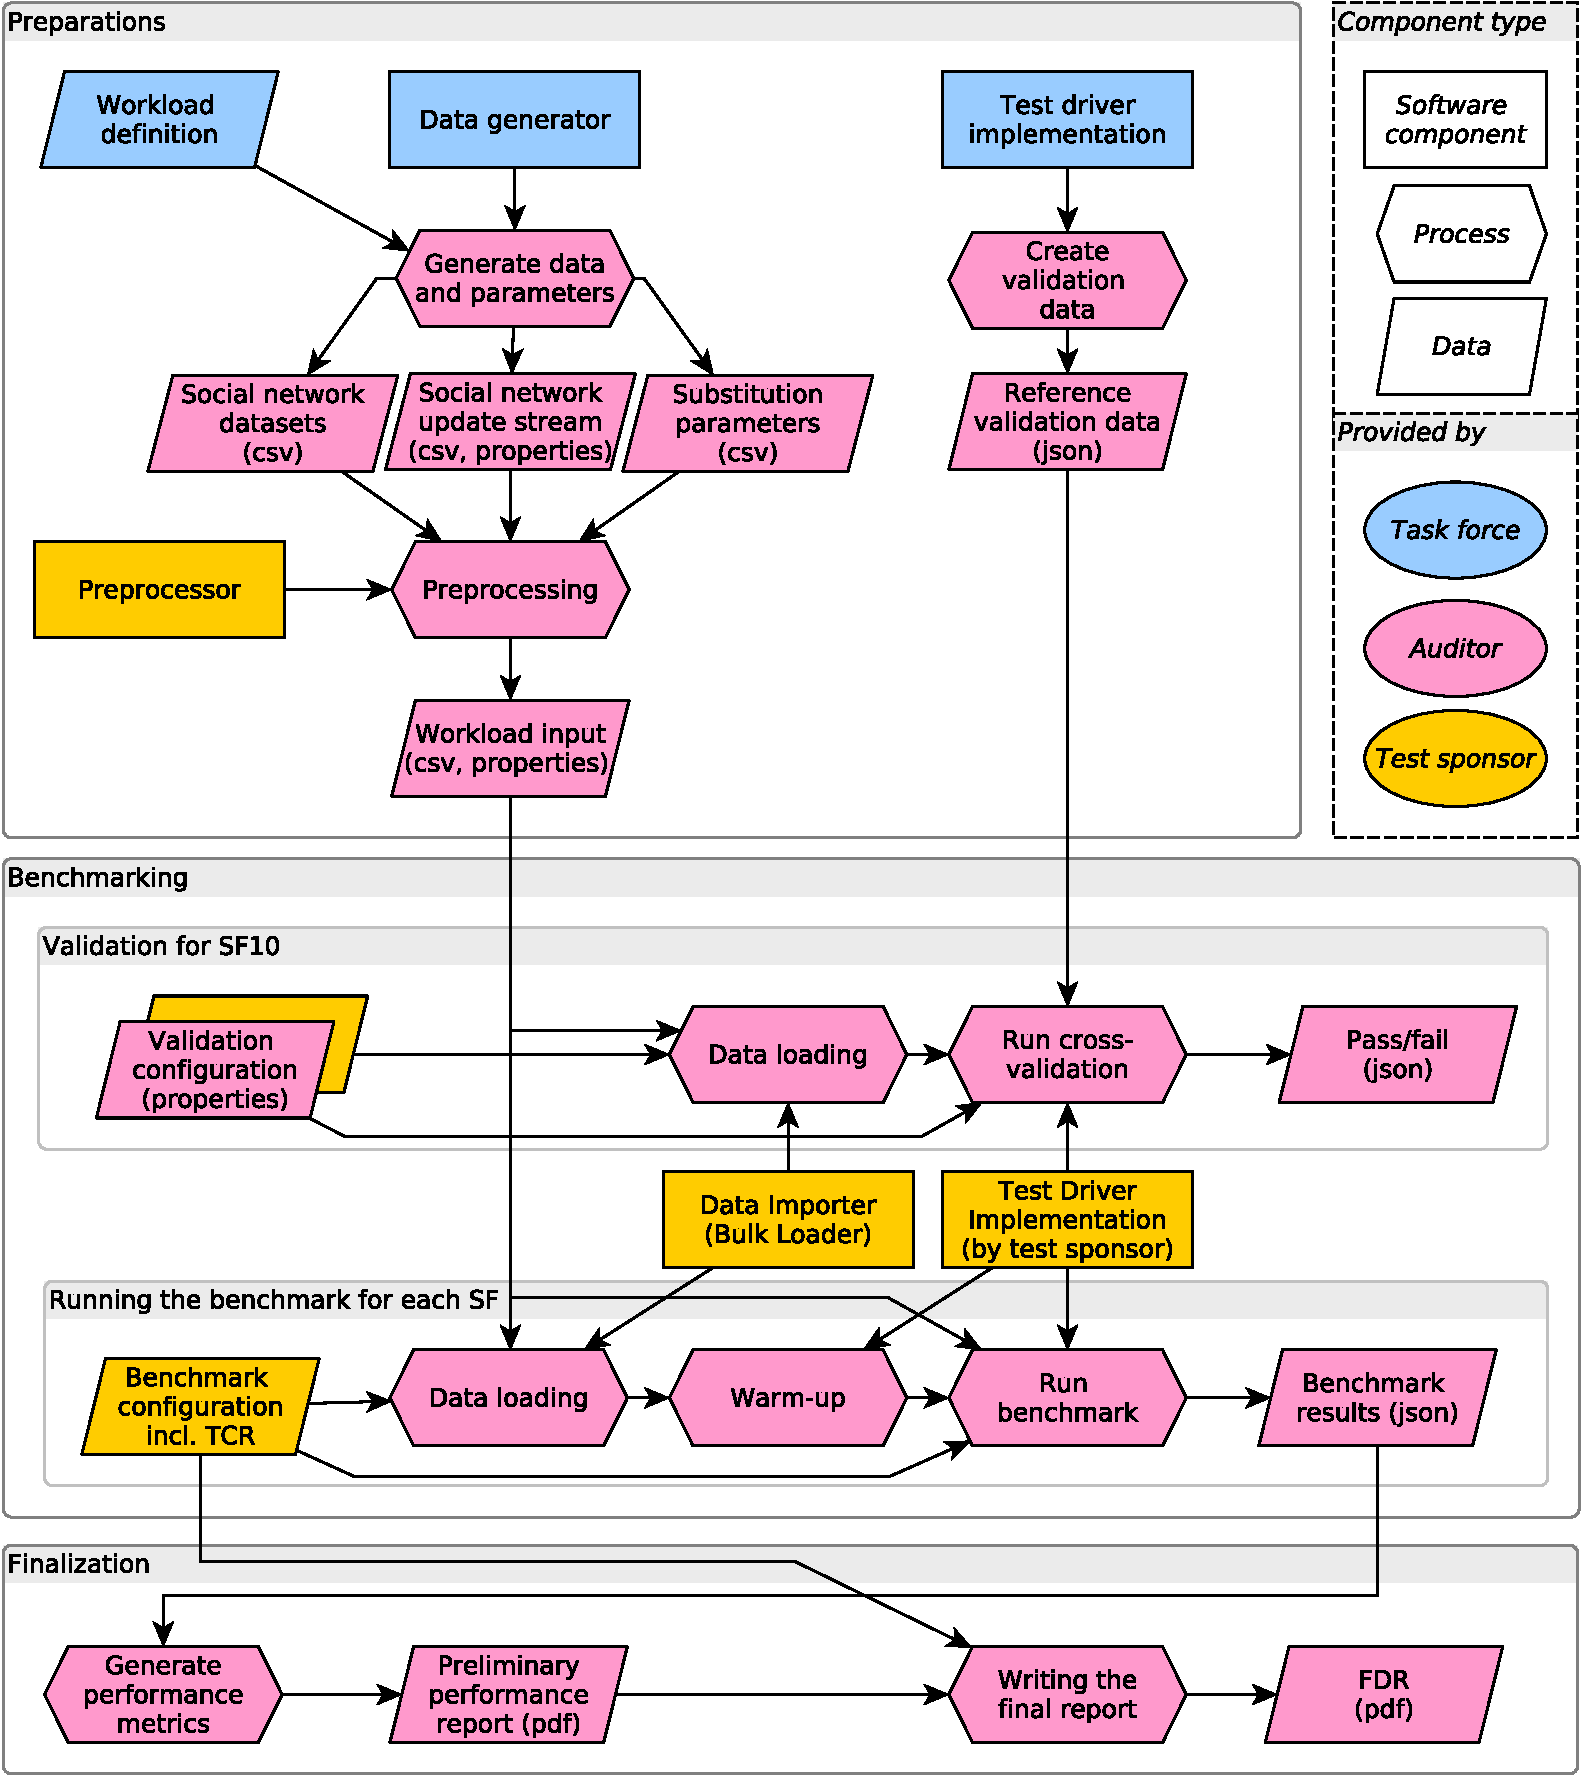
\includegraphics[scale=\yedscale]{figures/auditing-workflow}
    \caption{Benchmark execution and auditing workflow. For non-audited runs, the implementers perform the steps of the auditor.}
    \label{fig:audit-workflow}
\end{figure}

A key objective of the auditing guidelines for the Interactive workload is to \emph{allow a broad range of systems} to implement the benchmark.
Therefore, they do not impose constraints on the data model
(graph, relational, triple, \etc representations are allowed)
or on the query language
(both declarative and imperative languages are allowed).

\subsection{Scaling}
\label{sec:int-scaling}

\subsubsection{Scale Factors}

The scale factor of an SNB data set is the size of the data set in GiB of CSV (comma-separated values) files.
The size of a data set is characterized by scale factors: SF10, SF30, SF100 \etc (see \autoref{sec:scale-factors}).
All data sets contain data for three years of social network activity.

The \emph{validation run} shall be performed on the SF10 data set (see \autoref{sec:int-validation-data-set}) and use at least \numprint{100000} operations.
Note that the auditor may perform additional validation runs of the benchmark implementation using smaller data sets (\eg SF1) and issue queries.\footnote{%
An example test could be to issue complex reads with parameters such as \texttt{personId} and \texttt{messageId} selected from the \textsf{Person}/\textsf{Message} entities inserted from the update streams and cross-validate these against other systems. (The substitution parameters are taken from the initial snapshot of the graph so these nodes are not targeted by the regular workload executed by the driver.)%
}

Audited \emph{benchmark runs} of the Interactive workload shall use SF30 or larger data sets. The rationale behind this decision is to ensure that there is a sufficient number of update operations available to guarantee 2.5~hours of continuous execution (see \autoref{sec:int-measurement-window}).

% \begin{quote}
%     \emph{Rationale behind scaling.} The authors are aware that the prevalent practice for online benchmarks is to tie the reported throughput to the scale, \eg max 12.5 tpmC per warehouse in \mbox{TPC-C}. The authors depart from this practice here because with throughput tied to scale, test systems with interesting throughput rapidly become very expensive, raising the entry barrier for publishing a result. It is thought that scaling in buckets lowers the barrier of entry and reduces incentive to use hardware configurations that would be unusual in a production environment.
% \end{quote}
%COMMENTS FROM PAST GABOR TO FUTURE GABOR
%what it wants to say is that unlike TPC-C, you can get a large throughput (lots of ops) even on a small data set
%which is correct but we can ran out of updates due to the 2.5-hr simulation requirement
%so its (implied) conclusion does not hold fully hold for SNB interactive

\subsubsection{Social Network data sets}
\label{sec:int-data-sets}

\paragraph{Initial data set}
The data set is divided into a bulk loadable initial database population (90\%) and an update stream (10\%). These are generated by the SNB data generator. The data generator has options for splitting the data set into any number of files.

\paragraph{Dependencies between messages in the update stream}
The update stream contains the latest 10\% of the events in the simulated social network. These events form a single serializable sequence in time. Some events will depend on preceding events, for example a message must exist before a reply comment to the message is created. The data generator guarantees that these are separated by at least 10 seconds of simulation time.

\paragraph{Parallel updates}
The update stream may be broken into arbitrarily many sub-streams. The partition scheme is created by the \datagen. During benchmark execution, the driver preserves dependencies between update operations, such as ensuring not to refer to non-existent entities in updates (\eg a like is not added to a message which has not been inserted yet).

\subsection{Data Model and Data Loading}

\subsubsection{Supported Data Models}

SNB may be implemented with different data models (\eg relational, RDF, and different graph data models). The reference schema is provided in the specification using a UML-like notation. 


\subsubsection{Generated Input Data}
\label{sec:generated-data}

\paragraph{Storage}
The data generator produces comma-separated values (CSV) for all data models.

\paragraph{Data format}
A single attribute has a single data type, as follows:
\begin{description}
    \item [Identifier] This is an integer value foreign key or a URI in RDF. If this is an integer column, the implementation data type should support at least $2^{50}$ distinct values.
    \item [Date] A date should support a date range from 0000 to 9999 in the year field.
    \item [DateTime] A datetime should support a date range from 0000 to 9999 in the year field, with at least millisecond precision.
    \item [Short string] The string column for names may have a variable length and may have a declared maximum length, \eg 40 characters.
    \item [Long string] For example a message content may be a long string that is often short in the data but may not declare a maximum length and must support data sizes of up to 1~MB.
\end{description}

The above is stated in further detail in the benchmark specification, and it shall take precedence over the
above in the case of conflict.

A single attribute in the reference schema may not be divided into multiple attributes in the target schema.

\paragraph{Database schema}
A schema on the DBMS is optional. An RDF implementation for example may work without one. An RDF implementation is allowed to load the RDF reference schema and to take advantage of the data type and cardinality statements therein. 

\paragraph{Configuration parameters}
\datagen configuration parameters, including SF, distributions, number of persons, serialiser (\eg CsvSingularMergedFK) should be reported.

\paragraph{Primary data structures}
An RDF, relational, or graph schema may specify system specific options affecting DBMS storage layout. These may for example specify vertical partitioning. Vertical partitioning means anything from a column store layout with per-column allocated storage space to use of explicit column groups. Any mix of row or column-wise storage structures is allowed as long as this is declaratively specified on a per data structure-basis.

\paragraph{Auxiliary data structures}
Covering indices and clustered indices are allowed. If these are defined, then all replications of data implied by these must be maintained statement by statement, \ie each auxiliary data structure must be consistent with any other data structures of the table after each data manipulation operation.

A covering index is an index which materialises a specific order of a specific subset or possibly all columns of a table. 
A clustered index is an index which materialises all columns of a table in a specific order, which order may or may not be that of the primary key of the table. A clustered or covering index may be the primary or only representation of a table.

Any subset of the columns on a covering or clustered index may be used for ordering the data. A hash based index or a combination of a hash based and tree based index are all allowed, in row or column-wise or hybrid forms.

\paragraph{Loading the data}

We expect the SUT to provide some means to bulk load the data set either in the form of a dedicated offline loader component or an online loader that allows bulk inserting into a database.
The total of the bulk load time and the time for subsequent operations (indexing, computing statistics, \etc) must be reported in the FDR (see \autoref{sec:int-benchmark-workflow}).
As loading can be an expensive operation, it is allowed to conduct the audit such that the loading is only performend once, and the validation/benchmarking phases use the resulting database instance.
In practice, this can look like as follows:
(1)~load the data,
(2)~compute statistics, uniqueness constraints, keys, indices, \etc,
(3)~shut down the SUT,
(4)~create a backup of the database (\eg by copying the directory of the database).
For all subsequent runs, the database shall be restored from the backup.

\subsection{Precomputation}

Precomputation of query results (both interim and end results) is allowed. However, systems must ensure that precomputed results (\eg materialized views) are kept consistent upon updates.

\subsection{Benchmark Software Components}
\label{sec:snb-software-components}
LDBC provides a test driver, data generator, and summary reporting scripts. Benchmark implementations shall use a stable version (\eg 0.3.6) of the test driver. The SUT's database software should be a stable version that is available publicly or can be purchased at the time of the release of the audit.

\subsubsection{Adaptation of the Test Driver to a DBMS}
\label{sec:test-driver}
A qualifying run must use a test driver that adapts the provided test driver to interface with the SUT. Such an implementation, if needed, must be provided by the test sponsor. The parameter generation, result recording, and workload scheduling parts of the test driver should not be changed. The auditor must be given access to the test driver source code used in the reported run.

The test driver produces the following artefacts for each execution as a by product of the run: Start and end timestamps in wall clock time, recorded with microsecond precision. The identifier of the operation and any substitution parameters.


\subsubsection{Summary of Benchmark Results}
\label{sec:performance-metrics}
A separate test summary tool provided with the test driver analyses the test driver log(s) after a measurement window is completed. 

The tool produces for each of the distinct queries and transactions the following summary:
\begin{itemize}
    \item Run time of query in wall clock time.
    \item Count of executions.
    \item Minimum/mean/percentiles/maximum execution time.
    \item Standard deviation from the average execution time.
\end{itemize}
The tool produces for the complete run the following summary:
\begin{itemize}
    \item Operations per second for a given SF (throughput). This is the primary metric of this workload.
    \item The total execution time in wall clock time.
    \item The total number of completed operations.
\end{itemize}


\subsection{Implementation Language and Data Access Transparency}

The queries and updates may be implemented in a domain-specific query language or as procedural code written in a general-purpose programming language (\eg using the API of the database).

\subsubsection{Implementations Using a Domain-Specific Query Language}
\label{sec:snb-domain-specific-query-language}

If a domain-specific query language is used, \eg SPARQL, SQL, Cypher, or Gremlin, then explicit query plans are prohibited in all the read-only queries.%
\footnote{If the queries are not clearly declarative, the auditor must ensure that they do not specify explicit query plans by investigating their source code and experimenting with the query planner of the system (\eg using SQL's \texttt{EXPLAIN} command).}
The update transactions may still consist of multiple statements, effectively amounting to explicit plans.

Explicit query plans include but are not limited to:
\begin{itemize}
    \item Directives or hints specifying a join order or join type
    \item Directives or hints specifying an access path, \eg which index to use
    \item Directives or hints specifying an expected cardinality, selectivity, fanout or any other information that pertains to the expected number or results or cost of all or part of the query.
\end{itemize}

\begin{quote}
    \emph{Rationale behind the applied restrictions.} The updates are effectively OLTP and, therefore, the customary freedoms apply, including the use of stored procedures, however subject to access transparency. Declarative queries in a benchmark implementation should be such that they could plausibly be written by an application developer. Therefore, their formulation should not contain system specific aspects that an application developer would be unlikely to know. In other words, making a benchmark implementation should not require uncommon sophistication on behalf of the developer. This is regular practice in analytical benchmarks, \eg \mbox{TPC-H}.
\end{quote}

\subsubsection{Implementations Using a General-Purpose Programming Language}
\label{sec:snb-general-purpose-programming-language}

Implementations using a general-purpose programming language for specifying the queries (including procedural, imperative, and API-based implementations) are expected to respect the rules described in \autoref{sec:query-languages}.
For these implementations, the rules in \autoref{sec:snb-domain-specific-query-language} do not apply.

\subsection{Correctness of Benchmark Implementation}

\subsubsection{Validation data set}
\label{sec:int-validation-data-set}
The scale factor 10 shall be used as validation data set.

\subsubsection{ACID Compliance}
\label{sec:int-acid-compliance}

The Interactive workload requires full ACID support (\autoref{sec:acid-compliance}) from the SUT.
This is tested using the LDBC ACID test suite.
For the specification of this test suite, see \autoref{sec:acid-test-suite} and the related software repository at \url{https://github.com/ldbc/ldbc_acid}.

\paragraph{Expected level of isolation}
If a transaction reads the database with intent to update, the DBMS must guarantee that repeating the same read within the same transaction will return the same data. This also means that no more and no less data rows must be returned. In other words, this corresponds to snapshot or to serializable isolation. If the database is accessed without transaction context or without intent to update, then the DBMS should provide read committed semantics, \eg repeating the same read may produce different results but these results may never include effects of pending uncommitted transactions.

\paragraph{Durability and checkpoints}

A checkpoint is defined as the operation which causes data persisted in a transaction log to become durable outside of the transaction log. Specifically, this means that an SUT restart after instantaneous failure following the completion of the checkpoint may not have recourse to transaction log entries written before the end of the checkpoint.

A checkpoint typically involves a synchronisation barrier at which all data committed prior too the moment is required to be in durable storage that does not depend on the transaction log.
Not all DBMSs use a checkpointing mechanism for durability. For example a system may rely on redundant storage of data for durability guarantees against instantaneous failure of a single server.

The measurement window may contain a checkpoint. If the measurement window does not contain one, then the restart test will involve redoing all the updates in the window as part of the recovery test.

The timed window ends with an instantaneous failure of the SUT. Instantaneously killing all the SUT process(es) is adequate for simulating instantaneous failure. All these processes should be killed within one second of each other with an operating system action equivalent to the Unix \verb+kill -9+. If such is not available, then powering down each separate SUT component that has an independent power supply is also possible.

The restart test consists of restarting the SUT process(es) and finishes when the SUT is back online with all its functionality and the last successful update logged by the driver can be seen to be in effect in the database.
%In the case of a distributed (scale-out) system, a particular partition may be recovered whereas another one is still in the process of recovering. If this is so, then checking for the last update shall not be done until all partitions are online.

If the SUT hardware was powered down, the recovery period does not include the reboot and possible file system check time. The recovery time starts when the DBMS software is restarted.




\paragraph{Recovery} 
The SUT is to be restarted after the measurement window and the auditor will verify that the SUT contains the entirety of the last update recorded by the test driver(s) as successfully committed. The driver or the implementation have to make this information available. The auditor may also check the \emph{audit log} of the SUT (if available) to confirm that the operations issued by the driver were saved.

Once an official run has been validated, the recovery capabilities of the system must be tested. The system and the driver must be configured in the same way as in during the benchmark execution. After a warm-up period, an execution of the benchmark will be performed under the same terms as in the previous measured run.

\paragraph{Measuring recovery time}
At an arbitrary point close to 2 hours of wall clock time during the run, the machine will be shut down. Then, the auditor will restart the database system and will check that the last committed update (in the driver log file) is actually in the database. The auditor will measure the time taken by the system to recover from the failure. Also, all the information about how durability is ensured must be disclosed. If checkpoints are used, these must be performed with a period of 10 minutes at most.


\subsection{Benchmarking Workflow}
\label{sec:int-benchmark-workflow}

A benchmark execution is divided into the following processes (these processes are also shown in \autoref{fig:audit-workflow}):

\begin{description}
    \item[Generate data] This includes running the data generator, placing the generated files in a staging area, configuring storage, setting up the SUT configuration and preparing any data partitions in the SUT. This may include preallocating database space but may not include loading any data or defining any schema having to do with the benchmark. The \verb|ldbc.snb.interactive.update_interleave| driver parameter must come from the \verb|updateStream.properties| file, which is created by the data generator. That parameter should never be set manually. This parameter signifies the average distance of update operations in the workload.
    \item[Preprocessing] If needed, the output from the data generator is to preprocess the data set (\autoref{sec:auditing-data-format}).
    \item[Create validation data] Using one of the reference implementations of the benchmark, the reference validation data is obtained in .json format.
    \item[Data loading] The test sponsor must provide all the necessary documentation and scripts to load the data set into the database to test.
    This includes defining the database schema, if any, loading the initial database population, making this durably stored and gathering any optimiser statistics.
    The system under test must support the different data types needed by the benchmark for each of the attributes at their specified precision. No data can be filtered out, everything must be loaded. The test sponsor must provide a tool to perform arbitrary checks of the data or a shell to issue queries in a declarative language if the system supports it.
    \item[Run cross-validation] This step uses the data loader to populate the database, but the load is not timed. The validation data set is used to verify the correctness of the SUT. The auditor must load the provided data set and run the driver in validation mode, which will test that the queries provide the official results.  The benchmarking workflow will not go beyond this point unless results match the expected output.
    \item[Warm-up] Benchmark runs are preceded by a warm-up which must be performed using the LDBC driver.
    \item[Run benchmark] The bulk load time is reported and is equal to the amount of elapsed wall clock time between starting the schema definition and receiving the confirmation message of the end of statistics gathering. The workflow runs begin after the bulk load is completed. If the run does not directly follow the bulk load, it must start at a point in the update stream that has not previously been played into the database. In other words, a run may only include update events whose timestamp is later than the latest message creation date in the database prior to start of run. The run starts when the first of the test drivers send its first message to the SUT. If the SUT is running in the same process as the driver, the window starts
    when the driver starts. Also, make sure that the \verb|-rl/--results_log| is enabled. Make sure that all operations are enabled and the frequencies are those for the selected scale factor (see the exact specification of the frequencies in \autoref{sec:sf-statistics}).
\end{description}

\subsubsection{Query Timing During Benchmark Run}
\label{sec:ontime-requirements}
A valid benchmark run must last at least 2 hours of wall clock time and at most 2 hours and 15 minutes.
In order to be valid, a benchmark run needs to meet the ``95\% on-time requirement''.
The \texttt{results\_log.csv} file contains the $\mathsf{actual\_start\_time}$ and the $\mathsf{scheduled\_start\_time}$ of each of the issued queries. In order to have a valid run, 95\% of the queries must meet the following condition:
\begin{equation*}
\mathsf{actual\_start\_time} - \mathsf{scheduled\_start\_time} < 1\
\mathrm{second}
\end{equation*}

If the execution of the benchmark is valid, the auditor must retrieve all the files from directory specified by \verb|--results_dir| which includes configuration settings used, results log and results summary. All of which must be disclosed.

\subsubsection{Measurement Window}
\label{sec:int-measurement-window}

Benchmark runs execute the workload on the SUT in two phases (\autoref{fig:measurement-window-selection}).
First, the SUT must undergo a warm-up period that takes at least 30 minutes and at most 35 minutes. The goal of this is to put the system in a steady state which reflects how it would behave in a normal operating environment. The performance of the operations during warm-up is not considered.
Next, the SUT is benchmarked during a two-hour measurement window. Operation times are recorded and checked to ensure the ``95\% on-time requirement'' is satisfied.

\begin{figure}[h]
    \centering
    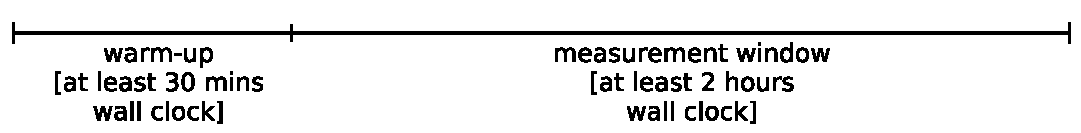
\includegraphics[width=.7\linewidth]{figures/measurement-window-selection}
    \caption{Warm-up and measurement window for benchmark run.}
    \label{fig:measurement-window-selection}
\end{figure}

The SNB \datagen produces 3~years worth data of which 10\% is used for updates (\autoref{sec:int-data-sets}), \ie approximately $3 \times 365 \times 0.1 = 109.5~\text{days} = 2628~\text{hours}$.
To ensure that the 2.5~hour wall clock period has enough input data, the lower bound of TCR is defined as 0.001 (if $2628$ hours of updates are played back at more than $1000\times$ speed, the benchmark framework runs out of updates to execute). System that can achieve a better compression (\ie lower TCR value) on a given scale factor should use larger SFs for their benchmark runs -- otherwise their total runs will be less than 2.5~hours, making them unsuitable for auditing.

%The test summary tool may be used for reading the logs created by a test driver.

\subsection{Full Disclosure Report}
\label{sec:int-fdr}

Upon successful completion of the audit, an FDR is compiled. In addition to the general requirements, the full disclosure shall cover the following:

\begin{itemize}
    \item General terms: an executive summary and declaration of the credibility of the audit
    \item System description and pricing summary: see \autoref{sec:system-config}
    \item Data generation and data loading: see \autoref{sec:generated-data}
    \item Test driver details: see \autoref{sec:test-driver}
    \item Performance metrics: see \autoref{sec:performance-metrics}
    \item Validation results: see \autoref{sec:int-validation-data-set}
    \item ACID compliance: see \autoref{sec:acid-compliance}
    \item List of supplementary materials
\end{itemize}

To ensure reproducibility of the audited results, a supplementary package is attached to the full disclosure report. This package should contain:

\begin{itemize}
    \item A README file with instructions specifying how to set up the system and run the benchmark
    \item Configuration files of the database, including database-level configuration such as buffer size and schema descriptors (if necessary)
    \item Source code or binary of a generic driver that can be used to interact with the DBMS
    \item SUT-specific LDBC driver implementation (similarly to the projects in \url{https://github.com/ldbc/ldbc_snb_interactive_v1_impls}, \url{https://github.com/ldbc/ldbc_snb_interactive_v2_impls}, \url{https://github.com/ldbc/ldbc_snb_bi})
    \item Script or instructions to compile the LDBC Java driver implementation
    \item Instructions on how to the reach the server through CLI and/or web UI (if applicable), \eg the URL (including port number), user name and password
    \item LDBC configuration files (\texttt{.properties}), including the \texttt{time\_compression\_ratio} values used in the audited runs
    \item Scripts to preprocess the input files (if necessary) and to load the data sets into the database
    \item Scripts to create validation data sets and to run the benchmark
    \item The implementations of the queries and the update operations, including their complete source code (\eg declarative queries specifications, stored procedures, \etc)
    \item Implementation of the ACID test suite
    \item Binary package of the DBMS (\eg \texttt{.deb} or \texttt{.rpm})
\end{itemize}



%%%%%%%%%%%%%%%%%%%%%%%%%%%%%%%%%%%%%%%%%%%%%%%%%%%%%%%%%%%%%%%%%%%%%%%%%%%%%%
%%%%%%%%%%%%%%%%%%%%%%%%%%%%%%%%%%%%%%%%%%%%%%%%%%%%%%%%%%%%%%%%%%%%%%%%%%%%%%
%%%%%%%%%%%%%%%%%%%%%%%%%%%%%%%%%%%%%%%%%%%%%%%%%%%%%%%%%%%%%%%%%%%%%%%%%%%%%%

\section{Auditing Rules for the Business Intelligence Workload}
\label{sec:auditing-bi-workload-audit}

%%%%%%%%%%%%%%%%%%%%%%%%%%%%%%%%%%%%%%%%%%%%%%%%%%%%%%%%%%%%%%%%%%%%%%%%%%%%%%
%%%%%%%%%%%%%%%%%%%%%%%%%%%%%%%%%%%%%%%%%%%%%%%%%%%%%%%%%%%%%%%%%%%%%%%%%%%%%%
%%%%%%%%%%%%%%%%%%%%%%%%%%%%%%%%%%%%%%%%%%%%%%%%%%%%%%%%%%%%%%%%%%%%%%%%%%%%%%

The following section describes the auditing rules specific to the Business Intelligence (BI) workload.

\subsection{Overview}
\label{sec:auditing-bi-audit-overview}

Implementing the BI workload requires the following key capabilities:

\begin{itemize}
    \item Loading the initial snapshot of the social network graph
    \item Evaluating the BI read queries (\autoref{sec:bi-reads})
    \item Evaluating the BI write operations: inserts (\autoref{sec:bi-insert-operations}) and deletes (\autoref{sec:bi-delete-operations})
    \item Performing concurrent reads and writes (\autoref{sec:auditing-bi-audit-workflow}) (optional, only allowed if ACID compliance is guaranteed)
\end{itemize}

\subsection{Workflow}
\label{sec:auditing-bi-audit-workflow}

\begin{figure}[htbp]
    \centering
    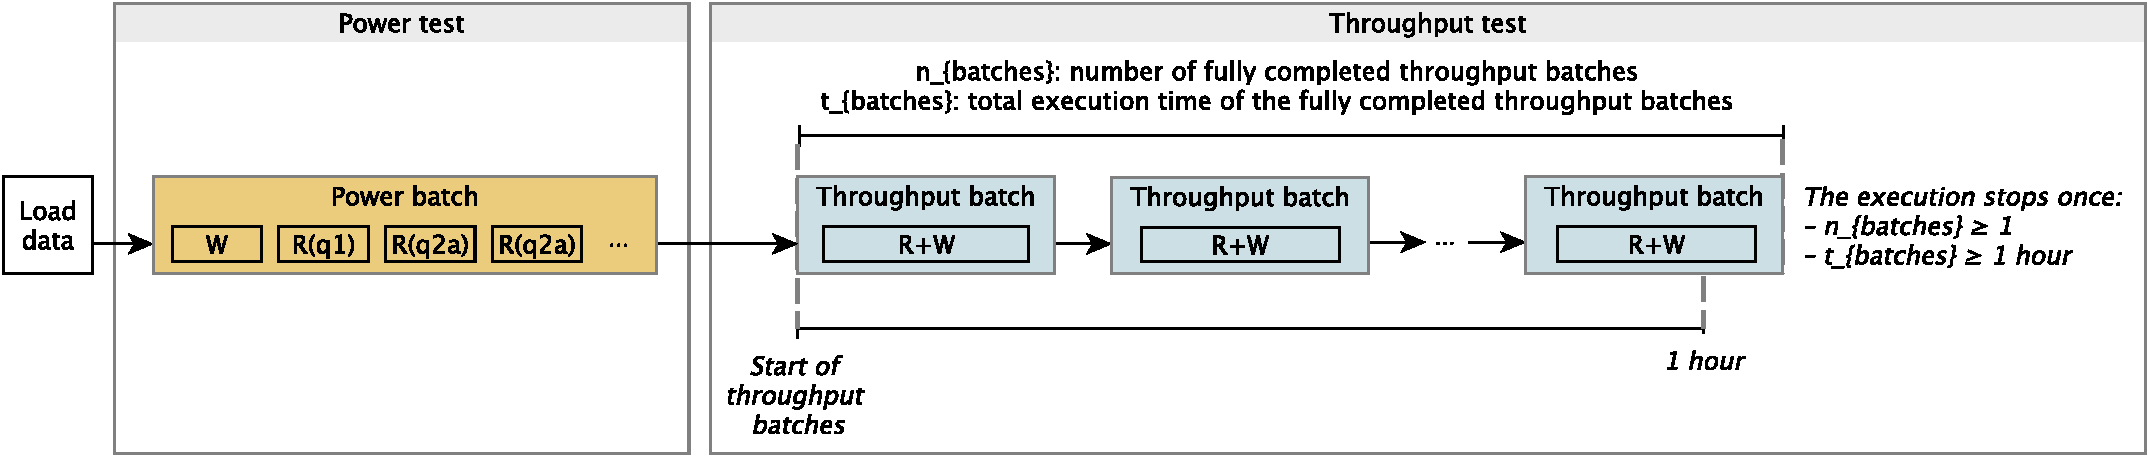
\includegraphics[scale=\yedscale]{figures/bi-batches.pdf}
    \caption{Tests and batches (power and throughput) executed in the BI workload's workflow.}
    \label{fig:bi-batches}
\end{figure}

The write operations and read queries are run in \emph{daily batches}.
In each batch, each query variant
(Q1, Q2\variantA, Q2\variantB, Q3, \ldots, Q20\variantA, Q20\variantB)
is executed using 30~different substitution parameters.
The BI workflow (\autoref{fig:bi-batches}) consists of two key parts:
the \emph{power test} (\autoref{sec:power-test}) and
the \emph{throughput test} (\autoref{sec:throughput-test}).

\subsubsection{Power Test}
\label{sec:power-test}

The \emph{power test} runs a single \emph{power batch}. This test first runs the write operations, followed by a sequential execution of individual read query variants.
The writes perform a day of inserts and deletes in the simulated social network,
while a total of $28 \times 30 = 840$ read queries are executed.

\subsubsection{Throughput Test}
\label{sec:throughput-test}

The \emph{throughput test} consists of multiple \emph{throughput batches}.
Each throughput batch runs the same type and the same amount of operations as the power batch.
However, they allow concurrent execution of the write operations and read queries in a given batch.

The execution of the throughput test during audits is the \emph{throughput measurement window}.
This window must span at least for 1~hour and
it must include at least one fully completed batch (see \autoref{fig:bi-batches}).

The workload defines two execution modes for the \emph{throughput batches}:

\begin{description}
    \item[Disjoint RW mode]
    In \emph{disjoint RW (read-write) mode} the system performs the reads and writes separately. It first executes the writes, then evaluates the read queries. Concurrency between the read operations is allowed.\\
    This mode is aimed at \emph{read-optimized data analytical systems} which do not support concurrent reads and writes. Implementations may also opt to use this mode for simplicity. For these implementations, passing the \emph{LDBC ACID compliance test} (\autoref{sec:acid-test-suite}) is not required.

    \item[Concurrent RW mode]
    In \emph{concurrent RW (read-write) mode} the system is allowed to run reads and writes concurrently. This requires the systems to be capable of handling \emph{transactions}. Implementations using this mode are required to pass the \emph{LDBC ACID compliance test} (\autoref{sec:acid-test-suite}).
\end{description}

\subsection{Runtimes}

The runtimes should be reported as follows:

\begin{itemize}
    \item The \emph{load time} ($t_\textit{load}$) denotes the time to load the data into the SUT and initialize auxiliary data structures (if applicable). For audited runs, we require that $t_\textit{load} < 24\textrm{ hours}$.
    \item The \emph{power test time} ($t_\textit{power test}$) denotes the time to perform the power test.
    \item The \emph{throughput measurement window time} ($t_\textit{throughput\ measurement}$) denotes the time to perform the throughput test, including the last (potentially unfinished) batch.
    \item The \emph{full throughput batches time} ($t_\textit{full\ throughput\ batches}$) denotes the time to evaluate the fully completed batches during the throughput measurement window.
\end{itemize}

Note that a warm-up period is not allowed (unlike the Interactive workload where such a period is required, see \autoref{sec:int-measurement-window}).

\subsection{Scoring Metrics}
\label{sec:auditing-bi-scoring-metrics}

SNBI BI provides four scoring metrics:
the \emph{power score}, the \emph{throughput score}, and their price-adjusted variants,
the \emph{per-\$ power score} and the \emph{per-\$ throughput score}.
All scores include the scale factor, denoted with ``@SF''.

\subsubsection{Price}
\label{sec:price-metrics}

We follow TPC's specification for reporting prices~\cite{tpc-pricing}.
The price is established as the \emph{total cost of ownership ($\textit{TCO}$)} for the SUT used in the benchmark,
reported as a breakdown of
machine cost,
software license costs,
and maintenance costs for 3 years.
In case of cloud deployments, the cost of running a 3-year reserved instance should be reported.
When establishing the price, the ``upfront payment'' option available at certain cloud providers should not be considered.

\subsubsection{Power Scores}
\label{sec:power-score}

The definition of \snbbi's power score follows \tpcH in using a geometric mean, ensuring that there is an incentive to improve all queries, no matter their running time.
Formally, the power score is based on the time to perform the writes
and
the time spent for executing each variant with 30~different substitution parameters, measured in seconds:
$$
\textit{power@SF} =
    \frac{\numprint{3600}}{\sqrt[29]{
        w
        \cdot q_{1}
        \cdot q_{2\variant{a}}
        \cdot q_{2\variant{b}}
        \cdot \ldots
        \cdot q_{18}
        \cdot q_{19\variant{a}}
        \cdot q_{19\variant{b}}
        \cdot q_{20\variant{a}}
        \cdot q_{20\variant{b}}
    }}
    \cdot
    \textit{SF}
$$

% Including all entries, the formula is:
% {\scriptsize
% $$
% \textit{power@SF} =
%     \frac{\numprint{3600}}{\sqrt[29]{
%         w
%         \! \cdot \! q_{1}
%         \! \cdot \! q_{2\variant{a}}
%         \! \cdot \! q_{2\variant{b}}
%         \! \cdot \! q_{2\variant{a}}
%         \! \cdot \! q_{2\variant{b}}
%         \! \cdot \! q_{3}
%         \! \cdot \! q_{4}
%         \! \cdot \! q_{5}
%         \! \cdot \! q_{6}
%         \! \cdot \! q_{7}
%         \! \cdot \! q_{8\variant{a}}
%         \! \cdot \! q_{8\variant{b}}
%         \! \cdot \! q_{9}
%         \! \cdot \! q_{10\variant{a}}
%         \! \cdot \! q_{10\variant{b}}
%         \! \cdot \! q_{11}
%         \! \cdot \! q_{12}
%         \! \cdot \! q_{13}
%         \! \cdot \! q_{14\variant{a}}
%         \! \cdot \! q_{14\variant{b}}
%         \! \cdot \! q_{15\variant{a}}
%         \! \cdot \! q_{15\variant{b}}
%         \! \cdot \! q_{16\variant{a}}
%         \! \cdot \! q_{16\variant{b}}
%         \! \cdot \! q_{17}
%         \! \cdot \! q_{18}
%         \! \cdot \! q_{19\variant{a}}
%         \! \cdot \! q_{19\variant{b}}
%         \! \cdot \! q_{20\variant{a}}
%         \! \cdot \! q_{20\variant{b}}
%     }}
%     \cdot
%     \textit{SF}
% $$
% }

To determine the price-adjusted power score, we factor in the $\textit{TCO}$\emph{:}
$$ \textit{power@SF/\$} = \textit{power@SF} \cdot \frac{\numprint{1000}}{\textit{TCO}} $$

\subsubsection{Throughput Scores}
\label{sec:throughput-score}

The throughput score is based on $t_\textit{load}$, measured in hours,
and the cumulative execution time and number of the throughput batches executed:
%throughput score is calculated as the number of batches the system could execute in a single day
$$
\textit{throughput@SF} =
    (24\text{ hours} - t_\textit{load})
    \cdot
    \frac{n_\textit{batches}}{t_\textit{batches}}
    \cdot
    \textit{SF}
$$

The subtraction of $t_\textit{load}$ ensures that the scoring rewards systems with efficient bulk loaders (unlike in \tpcH and \tpcDS which do not include load performance in their metrics).
The price-adjusted throughput score is determined analogously: % to the price-adjusted power score.
$$ \textit{throughput@SF/\$} = \textit{throughput@SF} \cdot \frac{\numprint{1000}}{\textit{TCO}} $$

\subsection{Implementation Rules}
\label{sec:auditing-bi-implementation-rules}

\subsubsection{Correctness}
\label{sec:auditing-bi-correcntess}

The SUT shall evaluate all operators correctly.
The auditor shall ascertain correctness on the SF10 data set. However, they are allowed to also use data sets of different scale factors, as well as issue custom operations (both reads and writes) to test for the correctness of the implemenation.

The validation of correctness is performed on the output of the \emph{power test} step.
The rationale for using this only step is that during concurrent execution of R/W operations in the \emph{throughput test}, it is not possible to guarantee deterministic query results, making validation impossible. Moreover, this step already includes a write batch, therefore the query results indirectly test the correctness of the implementation of write operations.

\subsubsection{Auxiliary Data Structures}
\label{sec:auditing-bi-auxiliary-data-structures}

Using auxiliary data structures (\eg indices, materialized views) is allowed if they are kept in an up-to-date state after each write operation. The full disclosure report should enumerate the auxiliary data structures used by the SUT. 

\subsubsection{Query Declarativity}
\label{sec:auditing-bi-query-declarativity}

Systems should use a domain-specific query language (\eg Cypher, Gremlin, GSQL) for the implementation, including the read queries and the update operations.
General-purpose programming languages (\eg C, C\texttt{++}, Java, Julia) are not allowed.

Implementations shall not use \emph{query-specific stored procedures written in a general-purpose programming language} (\eg a given procedure which implements BI Q5).
Using the stored procedure libraries considered to be the ``standard libraries'' of the SUT is allowed.%
\footnote{These libraries often include features such as weighted shortest path algorithms.}
Implementations may use \emph{stored procedures written in a domain-specific language}.
In cases when the categorization of the approach used by the SUT's query implementations is uncertain, it is the auditor's responsibility to decide whether the SUT complies with this rule.

\subsubsection{Query Variants}
\label{sec:auditing-bi-query-variants}

Several queries (\eg \queryRefCard{bi-read-14}{BI}{14}) use \variantA and \variantB variants with different sets of input parameters.
The SUT should not receive any hints on which variant it is currently evaluating (\eg Q14\variantA or Q14\variantB).
Moreover, it is not allowed for the query implementations to contain code that aims to detect the query variant used.

\subsection{Scaling}
\label{sec:auditing-bi-scaling}

Audited \emph{benchmark runs} of the BI workload shall use SF30 or larger data sets.
The rationale behind this decision is to ensure that there should be a sufficient number of write operations available to guarantee the execution during the duration of the measurement window (see \autoref{fig:bi-batches}).

\subsection{Full Disclosure Report}
\label{sec:auditing-bi-fdr}

The \emph{full disclosure report} (FDR) and the \emph{supplementary package} shall contain
the same information as for SNB Interactive (\autoref{sec:int-fdr}),
including, if applicable (\autoref{sec:auditing-bi-implementation-rules}), the ACID compliance report (\autoref{sec:acid-compliance}).


\chapter{Related Work}
\label{section:related-work}

%%%%%%%%%%%%%%%%%%%%%%%%%%%%%%%%%%%%%%%%%%%%%%%%%%%%%%%%%%%%%%%%%%%%%%%%%%%%%%
%%%%%%%%%%%%%%%%%%%%%%%%%%%%%%%%%%%%%%%%%%%%%%%%%%%%%%%%%%%%%%%%%%%%%%%%%%%%%%
%%%%%%%%%%%%%%%%%%%%%%%%%%%%%%%%%%%%%%%%%%%%%%%%%%%%%%%%%%%%%%%%%%%%%%%%%%%%%%

\paragraph*{Graph processing benchmarks.}

Recent graph benchmarking initiatives focus on three key areas:

\begin{enumerate}
\item transactional workloads consisting of interactive read and update queries (OLTP) aiming at graph databases that explore small portions of the graph in each query~\cite{DBLP:conf/cidr/BarahmandG13,DBLP:conf/sigmod/ArmstrongPBC13,DBLP:journals/ase/DayarathnaS14,DBLP:conf/sigmod/ErlingALCGPPB15,DBLP:journals/pvldb/LissandriniBV18},
\item graph analysis algorithms (\eg PageRank) computed in bulk, typically expressed in cluster frameworks with graph APIs, rather than high-level queries~\cite{DBLP:conf/hipc/BaderM05,DBLP:conf/bigdataconf/ElserM13,DBLP:conf/sc/NaiXTKL15,DBLP:journals/pvldb/IosupHNHPMCCSAT16},
\item pattern matching and inferencing on semantic data~\cite{DBLP:journals/ws/GuoPH05,DBLP:books/sp/virgilio09/SchmidtHMPL09,DBLP:conf/semweb/MorseyLAN11,DBLP:conf/semweb/AlucHOD14,DBLP:journals/sosym/SzarnyasIRV18}.
\end{enumerate}

A recent technical report~\cite{lissandrini17} compares graph databases.

The challenges of using benchmarks correctly are described in~\cite{DBLP:conf/sigmod/RaasveldtHGM18}.

The Interactive queries were used in paper~\cite{DBLP:conf/grades/PacaciZLO17} to compare the performance of Gremlin, Cypher, SQL and SPARQL query engines.

%%%%%%%%%%%%%%%%%%%%%%%%%%%%%%%%%%%%%%%%%%%%%%%%%%%%%%%%%%%%%%%%%%%%%%%%%%%%%%
%%%%%%%%%%%%%%%%%%%%%%%%%%%%%%%%%%%%%%%%%%%%%%%%%%%%%%%%%%%%%%%%%%%%%%%%%%%%%%
%%%%%%%%%%%%%%%%%%%%%%%%%%%%%%%%%%%%%%%%%%%%%%%%%%%%%%%%%%%%%%%%%%%%%%%%%%%%%%

%\section{Scalable Graph Generators}

%The \datagen component of SNB is a fork of the generator described in~\cite{DBLP:conf/tpctc/PhamBE12}.

%%%%%%%%%%%%%%%%%%%%%%%%%%%%%%%%%%%%%%%%%%%%%%%%%%%%%%%%%%%%%%%%%%%%%%%%%%%%%%
%%%%%%%%%%%%%%%%%%%%%%%%%%%%%%%%%%%%%%%%%%%%%%%%%%%%%%%%%%%%%%%%%%%%%%%%%%%%%%
%%%%%%%%%%%%%%%%%%%%%%%%%%%%%%%%%%%%%%%%%%%%%%%%%%%%%%%%%%%%%%%%%%%%%%%%%%%%%%

\paragraph*{LDBC publications.}

A detailed list of LDBC publications is curated at~\url{http://ldbcouncil.org/publications}.


\bibliographystyle{abbrv}
\bibliography{ldbc-snb}

\appendix

\chapter{Choke Points}

\chapter{Choke Points}
\label{sec:choke-points}

\newcommand{\tpcCard}[1]{\colorbox{lightgray}{\tt TPC-H #1}}
\newcommand{\cpSection}[4][]{%
	\subsection*{%
		CP-#2: [#3] #4%
		\ifthenelse{\equal{#1}{}}{}{\hfill \tpcCard{#1}}%
	}%
	\label{choke_point_#2}}

%%%%%%%%%%%%%%%%%%%%%%%%%%%%%%%%%%%%%%%%%%%%%%%%%%%%%%%%%%%%%%%%%%%%%%%%%%%%%%
%%%%%%%%%%%%%%%%%%%%%%%%%%%%%%%%%%%%%%%%%%%%%%%%%%%%%%%%%%%%%%%%%%%%%%%%%%%%%%
%%%%%%%%%%%%%%%%%%%%%%%%%%%%%%%%%%%%%%%%%%%%%%%%%%%%%%%%%%%%%%%%%%%%%%%%%%%%%%

\section*{Introduction}

Choke points are a superset of~\cite{LdbcDeliverable} with the exception of CP \chokePoint{7.1}, which was removed and replaced with a new choke point. The correlations between choke points and queries are displayed in \autoref{tab:query_choke_point}.

{
\setlength{\tabcolsep}{.1em}
% Template-based generation of the table showing choke point coverage by queries.
% Note that 'update' queries (DEL, INS) and their choke points (CP-9.x) are omitted from the table
\begin{table}[htbp]
\scriptsize
\centering
\begin{tabular}{|l|
    
        |c|
    
} \hline

    
        & \chokePoint{ {{- choke_point -}} }
    
 \\ \hline


    {#- only list queries that have at least on choke point -#}
    
        \hline
        \queryRefCard{ {{- query.0 -}} }{
            IC
            BI
            
        }{ {{- query.3 -}} }
        
            
                &  \yes  
            
         \\ \hline
    


\end{tabular}
\caption{Coverage of choke points by queries.}
\label{tab:query_choke_point}
\end{table}

}

%%%%%%%%%%%%%%%%%%%%%%%%%%%%%%%%%%%%%%%%%%%%%%%%%%%%%%%%%%%%%%%%%%%%%%%%%%%%%%
%%%%%%%%%%%%%%%%%%%%%%%%%%%%%%%%%%%%%%%%%%%%%%%%%%%%%%%%%%%%%%%%%%%%%%%%%%%%%%
%%%%%%%%%%%%%%%%%%%%%%%%%%%%%%%%%%%%%%%%%%%%%%%%%%%%%%%%%%%%%%%%%%%%%%%%%%%%%%

\section{Aggregation Performance}

%%%%%%%%%%%%%%%%%%%%%%%%%%%%%%%%%%%%%%%%%%%%%%%%%%%%%%%%%%%%%%%%%%%%%%%%%%%%%%

\cpSection[1.2]{1.1}{QOPT}{Interesting orders}

This choke point tests the ability of the query optimizer to exploit the interesting orders induced by some operators. Apart from clustered indexes providing key order, other operators also preserve or even induce tuple orderings.
Sort-based operators create new orderings, typically the probe-side of a hash join conserves its order, etc.

\subsubsection{Queries}
{\raggedright
\queryRefCard{bi-read-02}{BI}{2}
\queryRefCard{bi-read-04}{BI}{4}
\queryRefCard{bi-read-11}{BI}{11}
\queryRefCard{bi-read-17}{BI}{17}
\queryRefCard{bi-read-18}{BI}{18}
\queryRefCard{bi-read-19}{BI}{19}
\queryRefCard{interactive-complex-read-02}{IC}{2}
\queryRefCard{interactive-complex-read-09}{IC}{9}

}

%%%%%%%%%%%%%%%%%%%%%%%%%%%%%%%%%%%%%%%%%%%%%%%%%%%%%%%%%%%%%%%%%%%%%%%%%%%%%%

\cpSection[1.1]{1.2}{QEXE}{High cardinality group-by performance}

This choke point tests the ability of the execution engine to parallelize group-by's with a large number of groups. Some queries require performing large group-by's.
In such a case, if an aggregation produces a significant number of groups, intra-query parallelization can be exploited as each thread may make its own partial aggregation.
Then, to produce the result, these have to be re-aggregated. In order to avoid this, the tuples entering the aggregation operator may be partitioned by a hash of the grouping key and be sent to the appropriate partition.
Each partition would have its own thread so that only that thread would write the aggregation, hence avoiding costly critical sections as well. A high cardinality distinct modifier in a query is a special case of this choke point.
It is amenable to the same solution with intra-query parallelization and partitioning as the group-by.
We further note that scale-out systems have an extra incentive for partitioning since this will distribute the CPU and memory pressure over multiple machines, yielding better platform utilization and scalability.

\hyperref[sec:bi-read-15]{bi-read-15}
\hyperref[sec:bi-read-01]{bi-read-01}
\hyperref[sec:bi-read-05]{bi-read-05}
\hyperref[sec:bi-read-25]{bi-read-25}
\hyperref[sec:bi-read-21]{bi-read-21}
\hyperref[sec:bi-read-12]{bi-read-12}
\hyperref[sec:interactive-complex-read-09]{interactive-complex-read-09}
\hyperref[sec:bi-read-06]{bi-read-06}
\hyperref[sec:bi-read-07]{bi-read-07}
\hyperref[sec:bi-read-04]{bi-read-04}
\hyperref[sec:bi-read-14]{bi-read-14}
\hyperref[sec:bi-read-02]{bi-read-02}
\hyperref[sec:bi-read-13]{bi-read-13}
\hyperref[sec:bi-read-16]{bi-read-16}
\hyperref[sec:bi-read-09]{bi-read-09}
\hyperref[sec:bi-read-18]{bi-read-18}
\hyperref[sec:bi-read-10]{bi-read-10}


%%%%%%%%%%%%%%%%%%%%%%%%%%%%%%%%%%%%%%%%%%%%%%%%%%%%%%%%%%%%%%%%%%%%%%%%%%%%%%

\cpSection{1.3}{QOPT}{Top-k pushdown}

This choke point tests the ability of the query optimizer to perform optimizations based on top-$k$ selections. Many times queries demand for returning the top-$k$ elements based on some property.
Engines can exploit that once $k$ results are obtained, extra restrictions in a selection can be added based on the properties of the $k$th element currently in the top-$k$, being more restrictive as the query advances, instead of sorting all elements and picking the highest $k$.

\hyperref[sec:interactive-complex-read-01]{interactive-complex-read-01}


%%%%%%%%%%%%%%%%%%%%%%%%%%%%%%%%%%%%%%%%%%%%%%%%%%%%%%%%%%%%%%%%%%%%%%%%%%%%%%

\cpSection[1.3]{1.4}{QEXE}{Low cardinality group-by performance}

This choke point tests the ability to efficiently perform group-by evaluation
when only a very limited set of groups is available.  This can require special
strategies for parallelization, \eg pre-aggregation when possible. This case also allows using special strategies for grouping like using array lookup if the domain of keys is small.

\subsubsection{Queries}
{\raggedright
\queryRefCard{bi-read-02}{BI}{2}
\queryRefCard{bi-read-04}{BI}{4}
\queryRefCard{bi-read-05}{BI}{5}
\queryRefCard{bi-read-09}{BI}{9}
\queryRefCard{bi-read-16}{BI}{16}
\queryRefCard{bi-read-19}{BI}{19}
\queryRefCard{bi-read-22}{BI}{22}
\queryRefCard{interactive-complex-read-11}{IC}{11}

}

%%%%%%%%%%%%%%%%%%%%%%%%%%%%%%%%%%%%%%%%%%%%%%%%%%%%%%%%%%%%%%%%%%%%%%%%%%%%%%
%%%%%%%%%%%%%%%%%%%%%%%%%%%%%%%%%%%%%%%%%%%%%%%%%%%%%%%%%%%%%%%%%%%%%%%%%%%%%%
%%%%%%%%%%%%%%%%%%%%%%%%%%%%%%%%%%%%%%%%%%%%%%%%%%%%%%%%%%%%%%%%%%%%%%%%%%%%%%

\section{Join Performance}

%%%%%%%%%%%%%%%%%%%%%%%%%%%%%%%%%%%%%%%%%%%%%%%%%%%%%%%%%%%%%%%%%%%%%%%%%%%%%%

\cpSection[2.3]{2.1}{QOPT}{Rich join order optimization}

This choke point tests the ability of the query optimizer to find optimal join orders. A graph can be traversed in different ways. In the relational model, this is equivalent to different join orders.
The execution time of these orders may differ by orders of magnitude. Therefore, finding an efficient join (traversal) order is important, which in general, requires enumeration of all the possibilities.
The enumeration is complicated by operators that are not freely re-orderable like semi-, \mbox{anti-,} and outer-joins. Because of this difficulty most join enumeration algorithms do not enumerate all possible plans, and therefore can miss the optimal join order. Therefore, this choke point tests the ability of the query optimizer to find optimal join (traversal) orders.

{\raggedright\noindent\paragraph{Choke points.}
\queryRefCard{bi-read-02}{BI}{2}
\queryRefCard{bi-read-04}{BI}{4}
\queryRefCard{bi-read-05}{BI}{5}
\queryRefCard{bi-read-09}{BI}{9}
\queryRefCard{bi-read-10}{BI}{10}
\queryRefCard{bi-read-11}{BI}{11}
\queryRefCard{bi-read-19}{BI}{19}
\queryRefCard{bi-read-20}{BI}{20}
\queryRefCard{bi-read-21}{BI}{21}
\queryRefCard{bi-read-22}{BI}{22}
\queryRefCard{bi-read-24}{BI}{24}
\queryRefCard{bi-read-25}{BI}{25}
\queryRefCard{interactive-complex-read-01}{Interactive}{1}
\queryRefCard{interactive-complex-read-03}{Interactive}{3}
}

%%%%%%%%%%%%%%%%%%%%%%%%%%%%%%%%%%%%%%%%%%%%%%%%%%%%%%%%%%%%%%%%%%%%%%%%%%%%%%

\cpSection[2.4]{2.2}{QOPT}{Late projection}

This choke point tests the ability of the query optimizer to delay the projection of unneeded attributes until late in the execution. Queries where certain columns are only needed late in the query.
In such a situation, it is better to omit them from initial table scans, as fetching them later by row-id with a separate scan operator, which is joined to the intermediate query result, can save temporal space, and therefore I/O.
Late projection does have a trade-off involving locality, since late in the plan the tuples may be in a different order, and scattered I/O in terms of tuples/second is much more expensive than sequential I/O.
Late projection specifically makes sense in queries where the late use of these columns happens at a moment where the amount of tuples involved has been considerably reduced;
for example after an aggregation with only few unique group-by keys or a top-$k$ operator.

\hyperref[sec:interactive-complex-read-07]{interactive-complex-read-07}
\hyperref[sec:bi-read-05]{bi-read-05}
\hyperref[sec:bi-read-25]{bi-read-25}
\hyperref[sec:bi-read-12]{bi-read-12}
\hyperref[sec:interactive-complex-read-09]{interactive-complex-read-09}
\hyperref[sec:interactive-complex-read-02]{interactive-complex-read-02}
\hyperref[sec:bi-read-04]{bi-read-04}
\hyperref[sec:bi-read-14]{bi-read-14}
\hyperref[sec:bi-read-13]{bi-read-13}
\hyperref[sec:bi-read-11]{bi-read-11}


%%%%%%%%%%%%%%%%%%%%%%%%%%%%%%%%%%%%%%%%%%%%%%%%%%%%%%%%%%%%%%%%%%%%%%%%%%%%%%

\cpSection{2.3}{QOPT}{Join type selection}

This choke point tests the ability of the query optimizer to select the proper join operator type, which implies accurate estimates of cardinalities.
Depending on the cardinalities of both sides of a join, a hash or an index-based join operator is more appropriate.
This is especially important with column stores, where one usually has an index on everything. Deciding to use a hash join requires a good estimation of cardinalities on both the probe and build sides.
In TPC-H, the use of hash join is almost a foregone conclusion in many cases, since an implementation will usually not even define an index on foreign key columns.
There is a break even point between index and hash based plans, depending on the cardinality on the probe and build sides.

{\raggedright\noindent\paragraph{Choke points.}
\queryRefCard{bi-read-02}{BI}{2}
\queryRefCard{bi-read-05}{BI}{5}
\queryRefCard{bi-read-06}{BI}{6}
\queryRefCard{bi-read-07}{BI}{7}
\queryRefCard{bi-read-09}{BI}{9}
\queryRefCard{bi-read-10}{BI}{10}
\queryRefCard{bi-read-11}{BI}{11}
\queryRefCard{bi-read-13}{BI}{13}
\queryRefCard{bi-read-14}{BI}{14}
\queryRefCard{bi-read-15}{BI}{15}
\queryRefCard{bi-read-16}{BI}{16}
\queryRefCard{bi-read-17}{BI}{17}
\queryRefCard{bi-read-19}{BI}{19}
\queryRefCard{bi-read-21}{BI}{21}
\queryRefCard{bi-read-23}{BI}{23}
\queryRefCard{bi-read-24}{BI}{24}
\queryRefCard{interactive-complex-read-02}{Interactive}{2}
\queryRefCard{interactive-complex-read-04}{Interactive}{4}
\queryRefCard{interactive-complex-read-05}{Interactive}{5}
\queryRefCard{interactive-complex-read-07}{Interactive}{7}
\queryRefCard{interactive-complex-read-09}{Interactive}{9}
\queryRefCard{interactive-complex-read-10}{Interactive}{10}
\queryRefCard{interactive-complex-read-11}{Interactive}{11}


}

%%%%%%%%%%%%%%%%%%%%%%%%%%%%%%%%%%%%%%%%%%%%%%%%%%%%%%%%%%%%%%%%%%%%%%%%%%%%%%

\cpSection[2.2]{2.4}{QOPT}{Sparse foreign key joins}

This choke point tests the performance of join operators when the join is sparse. Sometimes joins involve relations where only a small percentage of rows in one of the tables is required to satisfy a join. When tables are larger, typical join methods can be sub-optimal. Partitioning the sparse table, using Hash Clustered indexes or implementing Bloom filter tests inside the join are techniques to improve the performance in such situations~\cite{DBLP:journals/csur/Graefe93}.

{\raggedright\noindent\paragraph{Choke points.}
\queryRefCard{bi-read-03}{BI}{3}
\queryRefCard{bi-read-04}{BI}{4}
\queryRefCard{bi-read-05}{BI}{5}
\queryRefCard{bi-read-09}{BI}{9}
\queryRefCard{bi-read-16}{BI}{16}
\queryRefCard{bi-read-19}{BI}{19}
\queryRefCard{bi-read-21}{BI}{21}
\queryRefCard{bi-read-23}{BI}{23}
\queryRefCard{bi-read-24}{BI}{24}
\queryRefCard{bi-read-25}{BI}{25}
\queryRefCard{interactive-complex-read-08}{Interactive}{8}
\queryRefCard{interactive-complex-read-11}{Interactive}{11}
}

%%%%%%%%%%%%%%%%%%%%%%%%%%%%%%%%%%%%%%%%%%%%%%%%%%%%%%%%%%%%%%%%%%%%%%%%%%%%%%

\cpSection{2.5}{QEXE}{Worst-case optimal joins}

This choke point tests the query engine's ability to use multi-way joins to evaluate cyclic queries which are required to efficiently compute some dense subgraphs such as the triangle, the 4-cycle, and the diamond. The absence of multi-way joins (\eg in traditional RDBMSs which only support binary joins), implies that join performance will be provably suboptimal.

\input{choke-points/cp-2-5}

%%%%%%%%%%%%%%%%%%%%%%%%%%%%%%%%%%%%%%%%%%%%%%%%%%%%%%%%%%%%%%%%%%%%%%%%%%%%%%
%%%%%%%%%%%%%%%%%%%%%%%%%%%%%%%%%%%%%%%%%%%%%%%%%%%%%%%%%%%%%%%%%%%%%%%%%%%%%%
%%%%%%%%%%%%%%%%%%%%%%%%%%%%%%%%%%%%%%%%%%%%%%%%%%%%%%%%%%%%%%%%%%%%%%%%%%%%%%

\section{Data Access Locality}

%%%%%%%%%%%%%%%%%%%%%%%%%%%%%%%%%%%%%%%%%%%%%%%%%%%%%%%%%%%%%%%%%%%%%%%%%%%%%%

\cpSection[3.3]{3.1}{QOPT}{Detecting correlation}

This choke point tests the ability of the query optimizer to detect data correlations and exploiting them. If a schema rewards creating clustered indexes, the question then is which of the date or data columns to use as key.
In fact it should not matter which column is used, as range-propagation between correlated attributes of the same table is relatively easy. One way is through the creation of multi-attribute histograms after detection of attribute correlation.
With MinMax indexes, range-predicates on any column can be translated into qualifying tuple position ranges. If an attribute value is correlated with tuple position, this reduces the area to scan roughly equally to predicate selectivity.

{\raggedright\noindent\paragraph{Choke points.}
\queryRefCard{bi-read-02}{BI}{2}
\queryRefCard{bi-read-03}{BI}{3}
\queryRefCard{bi-read-11}{BI}{11}
\queryRefCard{bi-read-12}{BI}{12}
\queryRefCard{bi-read-22}{BI}{22}
\queryRefCard{interactive-complex-read-03}{Interactive}{3}


}

%%%%%%%%%%%%%%%%%%%%%%%%%%%%%%%%%%%%%%%%%%%%%%%%%%%%%%%%%%%%%%%%%%%%%%%%%%%%%%

\cpSection{3.2}{STORAGE}{Dimensional clustering}

This choke point tests suitability of the identifiers assigned to entities by the storage system to better exploit data locality. A data model where each entity has a unique synthetic identifier,
\eg RDF or graph models, has some choice in assigning a value to this identifier.
The properties of the entity being identified may affect this, \eg type (label), other dependent properties,
\eg geographic location, date, position in a hierarchy, etc., depending on the application. Such identifier choice may create locality which in turn improves efficiency of compression or index access.

{\raggedright\noindent\paragraph{Queries.}
\queryRefCard{bi-read-01}{BI}{1}
\queryRefCard{bi-read-02}{BI}{2}
\queryRefCard{bi-read-03}{BI}{3}
\queryRefCard{bi-read-07}{BI}{7}
\queryRefCard{bi-read-10}{BI}{10}
\queryRefCard{bi-read-11}{BI}{11}
\queryRefCard{bi-read-13}{BI}{13}
\queryRefCard{bi-read-14}{BI}{14}
\queryRefCard{bi-read-15}{BI}{15}
\queryRefCard{bi-read-18}{BI}{18}
\queryRefCard{bi-read-21}{BI}{21}
\queryRefCard{bi-read-24}{BI}{24}
\queryRefCard{interactive-complex-read-02}{IC}{2}
\queryRefCard{interactive-complex-read-08}{IC}{8}
\queryRefCard{interactive-complex-read-09}{IC}{9}

}

%%%%%%%%%%%%%%%%%%%%%%%%%%%%%%%%%%%%%%%%%%%%%%%%%%%%%%%%%%%%%%%%%%%%%%%%%%%%%%

\cpSection{3.3}{QEXE}{Scattered index access patterns}

This choke point tests the performance of indexes when scattered accesses are performed. The efficiency of index lookup is very different depending on the locality of keys coming to the indexed access.
Techniques like vectoring non-local index accesses by simply missing the cache in parallel on multiple lookups vectored on the same thread may have high impact.
Also detecting absence of locality should turn off any locality dependent optimizations if these are costly when there is no locality. A graph neighbourhood traversal is an example of an operation with random access without predictable locality.

\subsubsection{Queries}
{\raggedright
\queryRefCard{bi-read-04}{BI}{4}
\queryRefCard{bi-read-05}{BI}{5}
\queryRefCard{bi-read-07}{BI}{7}
\queryRefCard{bi-read-08}{BI}{8}
\queryRefCard{bi-read-15}{BI}{15}
\queryRefCard{bi-read-16}{BI}{16}
\queryRefCard{bi-read-19}{BI}{19}
\queryRefCard{bi-read-21}{BI}{21}
\queryRefCard{bi-read-22}{BI}{22}
\queryRefCard{bi-read-23}{BI}{23}
\queryRefCard{bi-read-25}{BI}{25}
\queryRefCard{interactive-complex-read-05}{IC}{5}
\queryRefCard{interactive-complex-read-07}{IC}{7}
\queryRefCard{interactive-complex-read-08}{IC}{8}
\queryRefCard{interactive-complex-read-09}{IC}{9}
\queryRefCard{interactive-complex-read-10}{IC}{10}
\queryRefCard{interactive-complex-read-11}{IC}{11}
\queryRefCard{interactive-complex-read-12}{IC}{12}
\queryRefCard{interactive-complex-read-13}{IC}{13}
\queryRefCard{interactive-complex-read-14}{IC}{14}

}

%%%%%%%%%%%%%%%%%%%%%%%%%%%%%%%%%%%%%%%%%%%%%%%%%%%%%%%%%%%%%%%%%%%%%%%%%%%%%%
%%%%%%%%%%%%%%%%%%%%%%%%%%%%%%%%%%%%%%%%%%%%%%%%%%%%%%%%%%%%%%%%%%%%%%%%%%%%%%
%%%%%%%%%%%%%%%%%%%%%%%%%%%%%%%%%%%%%%%%%%%%%%%%%%%%%%%%%%%%%%%%%%%%%%%%%%%%%%

\section{Expression Calculation}

%%%%%%%%%%%%%%%%%%%%%%%%%%%%%%%%%%%%%%%%%%%%%%%%%%%%%%%%%%%%%%%%%%%%%%%%%%%%%%

\cpSection[4.2a]{4.1}{QOPT}{Common subexpression elimination}

This choke point tests the ability of the query optimizer to detect common sub-expressions and reuse their results. A basic technique helpful in multiple queries is common subexpression elimination (CSE).
CSE should recognize also that \lstinline{avg} aggregates can be derived afterwards by dividing a \lstinline{sum} by the \lstinline{count} when those have been computed.

\hyperref[sec:bi-read-01]{bi-read-01}
\hyperref[sec:interactive-complex-read-10]{interactive-complex-read-10}
\hyperref[sec:bi-read-03]{bi-read-03}


%%%%%%%%%%%%%%%%%%%%%%%%%%%%%%%%%%%%%%%%%%%%%%%%%%%%%%%%%%%%%%%%%%%%%%%%%%%%%%

\cpSection[4.2d]{4.2}{QOPT}{Complex boolean expression joins and selections}

This choke point tests the ability of the query optimizer to reorder the execution of boolean expressions to improve the performance. Some boolean expressions are complex, with possibilities for alternative optimal evaluation orders.
For instance, the optimizer may reorder conjunctions to test first those conditions with larger selectivity~\cite{DBLP:conf/vldb/Moerkotte98}.

{\raggedright\noindent\paragraph{Queries.}
\queryRefCard{bi-read-18}{BI}{18}
\queryRefCard{interactive-complex-read-10}{IC}{10}

}

%%%%%%%%%%%%%%%%%%%%%%%%%%%%%%%%%%%%%%%%%%%%%%%%%%%%%%%%%%%%%%%%%%%%%%%%%%%%%%

\cpSection{4.3}{QEXE}{Low overhead expressions interpretation}

This choke point tests the ability of efficiently evaluating simple expressions on a large number of values. A typical example could be simple arithmetic expressions, mathematical functions like floor and absolute or date functions like extracting a year.

\subsubsection{Queries}
{\raggedright
\queryRefCard{bi-read-03}{BI}{3}
\queryRefCard{bi-read-18}{BI}{18}
\queryRefCard{bi-read-23}{BI}{23}
\queryRefCard{bi-read-24}{BI}{24}

}

%%%%%%%%%%%%%%%%%%%%%%%%%%%%%%%%%%%%%%%%%%%%%%%%%%%%%%%%%%%%%%%%%%%%%%%%%%%%%%

\cpSection{4.4}{QEXE}{String matching performance}

This choke point tests the ability of efficiently evaluating complex string
matching expressions (\eg via regular expressions).

%\input{choke-points/cp-4-4}

%%%%%%%%%%%%%%%%%%%%%%%%%%%%%%%%%%%%%%%%%%%%%%%%%%%%%%%%%%%%%%%%%%%%%%%%%%%%%%
%%%%%%%%%%%%%%%%%%%%%%%%%%%%%%%%%%%%%%%%%%%%%%%%%%%%%%%%%%%%%%%%%%%%%%%%%%%%%%
%%%%%%%%%%%%%%%%%%%%%%%%%%%%%%%%%%%%%%%%%%%%%%%%%%%%%%%%%%%%%%%%%%%%%%%%%%%%%%

\section{Correlated Sub-queries}

%%%%%%%%%%%%%%%%%%%%%%%%%%%%%%%%%%%%%%%%%%%%%%%%%%%%%%%%%%%%%%%%%%%%%%%%%%%%%%

\cpSection[5.1]{5.1}{QOPT}{Flattening sub-queries}

This choke point tests the ability of the query optimizer to flatten execution plans when there are correlated sub-queries. Many queries have correlated sub-queries and their query plans can be flattened,
such that the correlated sub-query is handled using an equi-join, outer-join or anti-join.
In TPC-H Q21, for instance, there is an \lstinline{EXISTS} clause (for orders with more than one supplier) and a \lstinline{NOT EXISTS} clauses (looking for an item that was received too late).
To execute this query well, systems need to flatten both sub-queries, the first into an equi-join plan, the second into an anti-join plan.
Therefore, the execution layer of the database system will benefit from implementing these extended join variants.

The ill effects of repetitive tuple-at-a-time sub-query execution can also be mitigated if execution systems by using vectorized, or blockwise query execution, allowing to run sub-queries with thousands of input parameters instead of one.
The ability to look up many keys in an index in one API call creates the opportunity to benefit from physical locality, if lookup keys exhibit some clustering.

\hyperref[sec:interactive-complex-read-07]{interactive-complex-read-07}
\hyperref[sec:interactive-complex-read-10]{interactive-complex-read-10}
\hyperref[sec:interactive-complex-read-03]{interactive-complex-read-03}
\hyperref[sec:bi-read-25]{bi-read-25}
\hyperref[sec:bi-read-22]{bi-read-22}
\hyperref[sec:bi-read-21]{bi-read-21}
\hyperref[sec:interactive-complex-read-06]{interactive-complex-read-06}
\hyperref[sec:bi-read-19]{bi-read-19}


%%%%%%%%%%%%%%%%%%%%%%%%%%%%%%%%%%%%%%%%%%%%%%%%%%%%%%%%%%%%%%%%%%%%%%%%%%%%%%

\cpSection[5.3]{5.2}{QEXE}{Overlap between outer and sub-query}

This choke point tests the ability of the execution engine to reuse results when there is an overlap between the outer query and the sub-query. In some queries, the correlated sub-query and the outer query have the same joins and selections.
In this case, a non-tree, rather DAG-shaped~\cite{DBLP:conf/btw/NeumannM09} query plan would allow to execute the common parts just once, providing the intermediate result stream to both the outer query and correlated sub-query,
which higher up in the query plan are joined together (using normal query decorrelation rewrites).
As such, the benchmark rewards systems where the optimizer can detect this and the execution engine supports an operator that can buffer intermediate results and provide them to multiple parent operators.

\hyperref[sec:interactive-complex-read-10]{interactive-complex-read-10}
\hyperref[sec:bi-read-08]{bi-read-08}
\hyperref[sec:bi-read-22]{bi-read-22}


%%%%%%%%%%%%%%%%%%%%%%%%%%%%%%%%%%%%%%%%%%%%%%%%%%%%%%%%%%%%%%%%%%%%%%%%%%%%%%

\cpSection[5.2]{5.3}{QEXE}{Intra-query result reuse}

This choke point tests the ability of the execution engine to reuse sub-query results when two sub-queries are mostly identical.
Some queries have almost identical sub-queries, where some of their internal results can be reused in both sides of the execution plan, thus avoiding to repeat computations.

\hyperref[sec:bi-read-15]{bi-read-15}
\hyperref[sec:bi-read-05]{bi-read-05}
\hyperref[sec:bi-read-25]{bi-read-25}
\hyperref[sec:bi-read-22]{bi-read-22}
\hyperref[sec:bi-read-21]{bi-read-21}
\hyperref[sec:interactive-complex-read-01]{interactive-complex-read-01}
\hyperref[sec:interactive-complex-read-08]{interactive-complex-read-08}
\hyperref[sec:bi-read-03]{bi-read-03}


%%%%%%%%%%%%%%%%%%%%%%%%%%%%%%%%%%%%%%%%%%%%%%%%%%%%%%%%%%%%%%%%%%%%%%%%%%%%%%
%%%%%%%%%%%%%%%%%%%%%%%%%%%%%%%%%%%%%%%%%%%%%%%%%%%%%%%%%%%%%%%%%%%%%%%%%%%%%%
%%%%%%%%%%%%%%%%%%%%%%%%%%%%%%%%%%%%%%%%%%%%%%%%%%%%%%%%%%%%%%%%%%%%%%%%%%%%%%

\section{Parallelism and Concurrency}

%%%%%%%%%%%%%%%%%%%%%%%%%%%%%%%%%%%%%%%%%%%%%%%%%%%%%%%%%%%%%%%%%%%%%%%%%%%%%%

\cpSection[6.3]{6.1}{QEXE}{Inter-query result reuse}

This choke point tests the ability of the query execution engine to reuse results from different queries. Sometimes with a high number of streams a significant amount of identical queries emerge in the resulting workload.
The reason is that certain parameters, as generated by the workload generator, have only a limited amount of parameters bindings.
This weakness opens up the possibility of using a query result cache, to eliminate the repetitive part of the workload.
A further opportunity that detects even more overlap is the work on recycling, which does not only cache final query results, but also intermediate query results of a ``high worth''.
Here, worth is a combination of partial-query result size, partial-query evaluation cost, and observed (or estimated) frequency of the partial-query in the workload.

\hyperref[sec:bi-read-15]{bi-read-15}
\hyperref[sec:bi-read-05]{bi-read-05}
\hyperref[sec:interactive-complex-read-10]{interactive-complex-read-10}
\hyperref[sec:bi-read-12]{bi-read-12}
\hyperref[sec:bi-read-20]{bi-read-20}
\hyperref[sec:bi-read-07]{bi-read-07}
\hyperref[sec:bi-read-13]{bi-read-13}
\hyperref[sec:bi-read-03]{bi-read-03}
\hyperref[sec:bi-read-11]{bi-read-11}


%%%%%%%%%%%%%%%%%%%%%%%%%%%%%%%%%%%%%%%%%%%%%%%%%%%%%%%%%%%%%%%%%%%%%%%%%%%%%%
%%%%%%%%%%%%%%%%%%%%%%%%%%%%%%%%%%%%%%%%%%%%%%%%%%%%%%%%%%%%%%%%%%%%%%%%%%%%%%
%%%%%%%%%%%%%%%%%%%%%%%%%%%%%%%%%%%%%%%%%%%%%%%%%%%%%%%%%%%%%%%%%%%%%%%%%%%%%%

\section{RDF and Graph Specifics}

%%%%%%%%%%%%%%%%%%%%%%%%%%%%%%%%%%%%%%%%%%%%%%%%%%%%%%%%%%%%%%%%%%%%%%%%%%%%%%

\cpSection{7.1}{QEXE}{Incremental path computation}

This choke point tests the ability of the execution engine to reuse work across
graph traversals. For example, when computing paths within a range of distances,
it is often possible to incrementally compute longer paths by reusing paths of
shorter distances that were already computed.

{\raggedright\noindent\paragraph{Choke points.}
\queryRefCard{bi-read-16}{BI}{16}
\queryRefCard{interactive-complex-read-10}{Interactive}{10}


}

%%%%%%%%%%%%%%%%%%%%%%%%%%%%%%%%%%%%%%%%%%%%%%%%%%%%%%%%%%%%%%%%%%%%%%%%%%%%%%

\cpSection{7.2}{QOPT}{Cardinality estimation of transitive paths}

This choke point tests the ability of the query optimizer to properly estimate the cardinality of intermediate results when executing transitive paths. A transitive path may occur in a ``fact table'' or a ``dimension table'' position.
A transitive path may cover a tree or a graph, \eg descendants in a geographical hierarchy \vs graph neighbourhood or transitive closure in a many-to-many connected social network.
In order to decide proper join order and type, the cardinality of the expansion of the transitive path needs to be correctly estimated.
This could for example take the form of executing on a sample of the data in the
cost model or of gathering special statistics, \eg the depth and fan-out of a tree. In the case of hierarchical dimensions,
\eg geographic locations or other hierarchical classifications, detecting the cardinality of the transitive path will allow one to go to a star schema plan with scan of a fact table with a selective hash join.
Such a plan will be on the other hand very bad for example if the hash table is much larger than the ``fact table'' being scanned.

\subsubsection{Queries}
{\raggedright
\queryRefCard{bi-read-14}{BI}{14}
\queryRefCard{bi-read-16}{BI}{16}
\queryRefCard{bi-read-25}{BI}{25}
\queryRefCard{interactive-complex-read-12}{IC}{12}
\queryRefCard{interactive-complex-read-13}{IC}{13}
\queryRefCard{interactive-complex-read-14}{IC}{14}

}

%%%%%%%%%%%%%%%%%%%%%%%%%%%%%%%%%%%%%%%%%%%%%%%%%%%%%%%%%%%%%%%%%%%%%%%%%%%%%%

\cpSection{7.3}{QEXE}{Execution of a transitive step}

This choke point tests the ability of the query execution engine to efficiently execute transitive steps. Graph workloads may have transitive operations, for example finding a shortest path between nodes.
This involves repeated execution of a short lookup, often on many values at the
same time, while usually having an end condition, \eg the target node being reached or having reached the border of a search going in the opposite direction.
For the best efficiency, these operations can be merged or tightly coupled to
the index operations themselves. Also parallelization may be possible but may
need to deal with a global state, \eg set of visited nodes.
There are many possible tradeoffs between generality and performance

{\raggedright\noindent\paragraph{Choke points.}
\queryRefCard{bi-read-14}{BI}{14}
\queryRefCard{bi-read-16}{BI}{16}
\queryRefCard{bi-read-19}{BI}{19}
\queryRefCard{bi-read-25}{BI}{25}
\queryRefCard{interactive-complex-read-12}{Interactive}{12}
\queryRefCard{interactive-complex-read-13}{Interactive}{13}
\queryRefCard{interactive-complex-read-14}{Interactive}{14}
}

%%%%%%%%%%%%%%%%%%%%%%%%%%%%%%%%%%%%%%%%%%%%%%%%%%%%%%%%%%%%%%%%%%%%%%%%%%%%%%

\cpSection{7.4}{QEXE}{Efficient evaluation of termination criteria for transitive queries}

This tests the ability of a system to express termination criteria for transitive queries so that not the whole transitive relation has to be evaluated as well as efficient testing for termination.

\subsubsection{Queries}
{\raggedright
\queryRefCard{bi-read-14}{BI}{14}
\queryRefCard{bi-read-19}{BI}{19}

}

%%%%%%%%%%%%%%%%%%%%%%%%%%%%%%%%%%%%%%%%%%%%%%%%%%%%%%%%%%%%%%%%%%%%%%%%%%%%%%
%%%%%%%%%%%%%%%%%%%%%%%%%%%%%%%%%%%%%%%%%%%%%%%%%%%%%%%%%%%%%%%%%%%%%%%%%%%%%%
%%%%%%%%%%%%%%%%%%%%%%%%%%%%%%%%%%%%%%%%%%%%%%%%%%%%%%%%%%%%%%%%%%%%%%%%%%%%%%

\section{Language Features}


%%%%%%%%%%%%%%%%%%%%%%%%%%%%%%%%%%%%%%%%%%%%%%%%%%%%%%%%%%%%%%%%%%%%%%%%%%%%%%

\cpSection{8.1}{LANG}{Complex patterns}

\paragraph{Description}

A natural requirement for graph query systems is to be able to express complex
graph patterns.

\paragraph{Transitive edges.} Transitive closure-style computations are common in graph query systems, both with fixed bounds
(\eg get nodes that can be reached through at least 3 and at most 5 \textsf{knows} edges),
and without fixed bounds
(\eg get all \textsf{Messages} that a \textsf{Comment} replies to).

\paragraph{Negative edge conditions.} Some queries define \emph{negative pattern conditions}. For example, the condition that a certain \textsf{Message} does not have a certain \textsf{Tag} is represented in the graph as the absence of a \textsf{hasTag} edge between the two nodes. Thus, queries looking for cases where this condition is satisfied check for negative patterns, also known as negative application conditions (NACs) in graph transformation literature~\cite{DBLP:journals/fuin/HabelHT96}.

\paragraph{Language-specific notes}

Negative edge conditions are often difficult to express in early stage graph query languages. Notably, this is showcased by the fact that early versions of both the SPARQL and Cypher languages used cumbersome syntax to express such conditions.

\begin{description}
\item[Cypher.]
Prior to Neo4j version 2.0, Cypher queries used a syntax such as the following:

\begin{minipage}{\linewidth}
\begin{lstlisting}[language=cypher]
MATCH (source)-[r?:someType]->(target)
WHERE r IS NULL
RETURN source
\end{lstlisting}
\end{minipage}

In Neo4j 2.0, the \lstinline[language=cypher]{OPTIONAL MATCH} clause was introduced:\footnote{\url{https://dzone.com/articles/new-neo4j-optional}}

\begin{minipage}{\linewidth}
\begin{lstlisting}[language=cypher]
MATCH (source)
OPTIONAL MATCH (source)-[r:someType]->(target)
WHERE r IS NULL
RETURN source
\end{lstlisting}
\end{minipage}

However, the preferred method is to use a pattern condition in the \lstinline[language=cypher]{WHERE} clause:

\begin{minipage}{\linewidth}
\begin{lstlisting}[language=cypher]
MATCH (source)
WHERE NOT (source)-[:someType]->(target)
RETURN source
\end{lstlisting}
\end{minipage}

\item[SPARQL.]
Prior to SPARQL 1.1, queries with negative edge conditions could be expressed with the following approach:

\begin{minipage}{\linewidth}
\begin{lstlisting}[language=sparql]
OPTIONAL {
  ?xRoute ?routeDefinition ?xSensor .
  FILTER (sameTerm(base:routeDefinition, routeDefinition))
} .
FILTER (!bound(?routeDefinition))
\end{lstlisting}
\end{minipage}

Since SPARQL 1.1, the preferred method is using the \lstinline[language=sparql]{NOT EXISTS} construct.

\begin{minipage}{\linewidth}
\begin{lstlisting}[language=sparql]
?xSensor rdf:type base:Sensor .
?xRoute base:switchPosition ?xSwitchPosition .
FILTER NOT EXISTS { xRoute ?routeDefinition ?xSensor } .
\end{lstlisting}
\end{minipage}

The \lstinline{MINUS} construct can also be used for defining a negative condition for a single edge.\footnote{For details, see the ``Relationship and differences between \lstinline[language=sparql]{NOT EXISTS} and \lstinline[language=sparql]{MINUS}'' section in the SPARQL 1.1 specification at \url{https://www.w3.org/TR/sparql11-query/\#neg-notexists-minus}}

\begin{minipage}{\linewidth}
\begin{lstlisting}[language=sparql]
?xSensor rdf:type base:Sensor .
?xRoute base:switchPosition ?xSwitchPosition .
MINUS { xRoute ?routeDefinition ?xSensor } .
\end{lstlisting}
\end{minipage}

\end{description}

% https://stackoverflow.com/questions/10952332/return-node-if-relationship-is-not-present/14254214

{\raggedright\noindent\paragraph{Queries.}
\queryRefCard{bi-read-01}{BI}{1}

}

%%%%%%%%%%%%%%%%%%%%%%%%%%%%%%%%%%%%%%%%%%%%%%%%%%%%%%%%%%%%%%%%%%%%%%%%%%%%%%

\cpSection{8.2}{LANG}{Complex aggregations}

\paragraph{Description}

BI workloads are heavy on aggregation, including queries with \emph{subsequent
aggregations}, where the results of an aggregation serves as the input of
another aggregation. Expressing such operations requires some sort of query
composition or chaining (see also CP-8.4). It is also common to \emph{filter on
aggregation results} (similarly to the \lstinline[language=sql]{HAVING} keyword of SQL).

\paragraph{Language-specific notes}

\begin{description}
\item[Cypher.] Cypher does not allow aggregations on aggregations, \eg \lstinline[language=cypher]{avg(count(x))}, as the semantics of such expressions is not meaningful. However, it allows multiple aggregations is subsequent \lstinline[language=cypher]{WITH} and  \lstinline[language=cypher]{RETURN} clauses. There were multiple discussion rounds on the aggregation semantics of the openCypher language.\footnote{\url{http://www.opencypher.org/blog/2017/07/27/ocig1-aggregations-blog/}}

\item[SPARQL.] SPARQL requires users to explicitly enumerate variables in the \lstinline[language=sql]{GROUP BY} clause (similarly to SQL).
\end{description}

\subsubsection{Queries}
{\raggedright
\queryRefCard{bi-read-02}{BI}{2}
\queryRefCard{bi-read-03}{BI}{3}
\queryRefCard{bi-read-04}{BI}{4}
\queryRefCard{bi-read-05}{BI}{5}
\queryRefCard{bi-read-06}{BI}{6}
\queryRefCard{bi-read-07}{BI}{7}
\queryRefCard{bi-read-09}{BI}{9}
\queryRefCard{bi-read-10}{BI}{10}
\queryRefCard{bi-read-15}{BI}{15}
\queryRefCard{bi-read-18}{BI}{18}
\queryRefCard{bi-read-21}{BI}{21}
\queryRefCard{bi-read-25}{BI}{25}
\queryRefCard{interactive-complex-read-01}{IC}{1}
\queryRefCard{interactive-complex-read-03}{IC}{3}
\queryRefCard{interactive-complex-read-04}{IC}{4}
\queryRefCard{interactive-complex-read-05}{IC}{5}
\queryRefCard{interactive-complex-read-06}{IC}{6}
\queryRefCard{interactive-complex-read-12}{IC}{12}

}

%%%%%%%%%%%%%%%%%%%%%%%%%%%%%%%%%%%%%%%%%%%%%%%%%%%%%%%%%%%%%%%%%%%%%%%%%%%%%%

\cpSection{8.3}{LANG}{Ranking-style queries}

\paragraph{Description}

Additionally to aggregations, BI workloads often use \emph{window functions},
which perform aggregations without grouping input tuples to a single output
tuple.  A common use case for windowing is \emph{ranking}, \ie selecting the top
element with additional values in the tuple (nodes, edges or
attributes).\footnote{PostgreSQL defines the \lstinline[language=sql]{OVER}
keyword to use aggregation functions as window functions, and the
\lstinline[language=sql]{rank()} function to produce numerical ranks, see
\url{https://www.postgresql.org/docs/9.1/static/tutorial-window.html} for
details.}

\paragraph{Language-specific notes}

\begin{description}
\item[Cypher.]
Ranking can be expressed in Cypher as a sequence of ordering, collecting results and taking the top-$k$ values of the result list.\\

\noindent\begin{minipage}{\linewidth}
\begin{lstlisting}[language=cypher]
...
WITH x, ...
ORDER BY x
WITH collect(x) AS xs
WITH xs[0] AS top, xs[0..5] AS top5
...
\end{lstlisting}
\end{minipage}

\item[SPARQL.] SPARQL~1.0 allows simple top-$k$ queries. SPARQL~1.1 introduced scoring functions that can define a variable to be used for ordering~\cite{DBLP:conf/semweb/MagliacaneBV12}.
\emph{Window functions} are not yet supported but are under consideration for SPARQL~1.2\footnote{\url{https://github.com/w3c/sparql-12/issues/47}}.

%Simple top-k queries can be expressed in SPARQL 1.0 by including the ORDER BY and LIMIT clauses, which impose an order on the result set and limit the number of results. SPARQL 1.1 additionally enables the specification of complex scoring functions through the use of projection expressions that can define a variable to be used in the ORDER BY clause.
\end{description}

\subsubsection{Queries}
{\raggedright
\queryRefCard{bi-read-11}{BI}{11}
\queryRefCard{bi-read-13}{BI}{13}
\queryRefCard{bi-read-18}{BI}{18}
\queryRefCard{bi-read-22}{BI}{22}
\queryRefCard{bi-read-25}{BI}{25}
\queryRefCard{interactive-complex-read-07}{IC}{7}
\queryRefCard{interactive-complex-read-14}{IC}{14}

}

%%%%%%%%%%%%%%%%%%%%%%%%%%%%%%%%%%%%%%%%%%%%%%%%%%%%%%%%%%%%%%%%%%%%%%%%%%%%%%

\cpSection{8.4}{LANG}{Query composition}

\paragraph{Description}

Numerous use cases require \emph{composition} of queries, including the reuse of
query results (\eg nodes, edges) or using scalar subqueries (\eg selecting a
threshold value with a subquery and using it for subsequent filtering
operations).

\paragraph{Language-specific notes}

\begin{description}
\item[Cypher.] Nested subqueries were accepted in the openCypher language.\footnote{\url{https://github.com/petraselmer/openCypher/blob/1ca70bf8e3cea65ee47ce49eeabea83530eb529b/cip/1.accepted/CIP2016-06-22-nested-updating-and-chained-subqueries.adoc}}. Neo4j 4.1 introduced support for correlated subqueries.
\item[SPARQL.] SPARQL fully supports query composition.\footnote{\url{https://www.w3.org/TR/sparql11-query/\#subqueries}}
\end{description}

\subsubsection{Queries}
{\raggedright
\queryRefCard{bi-read-05}{BI}{5}
\queryRefCard{bi-read-10}{BI}{10}
\queryRefCard{bi-read-15}{BI}{15}
\queryRefCard{bi-read-18}{BI}{18}
\queryRefCard{bi-read-21}{BI}{21}
\queryRefCard{bi-read-22}{BI}{22}
\queryRefCard{bi-read-25}{BI}{25}

}

%%%%%%%%%%%%%%%%%%%%%%%%%%%%%%%%%%%%%%%%%%%%%%%%%%%%%%%%%%%%%%%%%%%%%%%%%%%%%%

\cpSection{8.5}{LANG}{Dates and times}

\paragraph{Description}

Handling dates and times is a fundamental requirement for production-ready
database systems. It is particularly important in the context of BI queries as
these often calculate aggregations on certain periods of time (\eg on entities created during the course of a month).

\paragraph{Language-specific notes}

\begin{description}
\item[Cypher.] The openCypher project has accepted a proposal to support dates and times.\footnote{\url{https://github.com/thobe/openCypher/blob/06accdb3e69820cdfac3dbd50a4f8eee73ba179a/cip/1.accepted/CIP2015-08-06-date-time.adoc}} Neo4j has datetime support since version 3.4.

\item[SPARQL.] SPARQL supports dates and times extensively with timezones and functions for extracting a part of a given date.\footnote{\url{https://www.w3.org/TR/sparql11-query/\#func-date-time}}
\end{description}

{\subsubsection{Queries}
\raggedright
\queryRefCard{bi-read-01}{BI}{1}
\queryRefCard{bi-read-02}{BI}{2}
\queryRefCard{bi-read-03}{BI}{3}
\queryRefCard{bi-read-10}{BI}{10}
\queryRefCard{bi-read-12}{BI}{12}
\queryRefCard{bi-read-13}{BI}{13}
\queryRefCard{bi-read-14}{BI}{14}
\queryRefCard{bi-read-18}{BI}{18}
\queryRefCard{bi-read-19}{BI}{19}
\queryRefCard{bi-read-21}{BI}{21}
\queryRefCard{bi-read-23}{BI}{23}
\queryRefCard{bi-read-24}{BI}{24}
\queryRefCard{bi-read-25}{BI}{25}

}

%%%%%%%%%%%%%%%%%%%%%%%%%%%%%%%%%%%%%%%%%%%%%%%%%%%%%%%%%%%%%%%%%%%%%%%%%%%%%

\cpSection{8.6}{LANG}{Handling paths}

\paragraph{Description}

\paragraph{Note on terminology.} The \emph{Glossary of graph theory terms} page of Wikipedia\footnote{\url{https://en.wikipedia.org/wiki/Glossary_of_graph_theory_terms}} defines \emph{paths} as follows: ``A path may either be a walk (a sequence of nodes and edges, with both endpoints of an edge appearing adjacent to it in the sequence) or a simple path (a walk with no repetitions of nodes or edges), depending on the source.''
In this work, we use the first definition, which is more common in modern graph database systems and is also followed in a recent survey on graph query languages~\cite{DBLP:journals/csur/AnglesABHRV17}.

Handling paths as first-class citizens is one of the key distinguishing features of graph database 
systems~\cite{DBLP:conf/sigmod/AnglesABBFGLPPS18}. Hence, additionally to
reachability-style checks, a language should be able to express
queries that operate on elements of a path, \eg calculate a score on each edge
of the path.
Also, some use cases specify uniqueness constraints on paths~\cite{DBLP:journals/csur/AnglesABHRV17}:
\emph{arbitrary path},
\emph{shortest path},
\emph{no-repeated-node semantics} (also known as \emph{simple paths}), and
\emph{no-repeated-edge semantics} (also known as \emph{trails}).
Other variants are also used in rare cases, such as \emph{maximal} (non-expandable) or \emph{minimal} (non-contractable) paths.

\paragraph{Language-specific notes}

\begin{description}
\item[Cypher.] Cypher uses \emph{no-repeated-edge matching semantics} (in return, this semantics is sometimes dubbed as \emph{cyphermorphism}).
Configurable matching semantics (\eg \lstinline[language=cypher]{MATCH ALL WALKS}) were proposed in the openCypher language.\footnote{\url{https://github.com/boggle/openCypher/blob/c139130b49aebe6a85fc395e2cf03cfeec8484c6/cip/1.accepted/CIP2017-01-18-configurable-pattern-matching-semantics.adoc}}
Regular path queries (RPQs) are also proposed in the openCypher language as \emph{path patterns}.\footnote{\url{https://github.com/thobe/openCypher/blob/b95eec108ce4ec07eedfe13b3e5fff0e94f789a4/cip/1.accepted/CIP2017-02-06-Path-Patterns.adoc}}

\item[SPARQL.] SPARQL uses \emph{homomorphism-based matching semantics} and supports RPQs as \emph{property paths}. Isomorphism-based matching semantics can be expressed by introducing custom filtering condition, \eg \lstinline[language=sparql]{FILTER ( ?e1 != ?e2 )}.

\item[G-CORE.] The \mbox{G-CORE} language~\cite{DBLP:conf/sigmod/AnglesABBFGLPPS18} treats paths as \emph{first-order citizens}: its \emph{path property graph data model} can store paths in the graph model with labels and properties. However, it only supports shortest path semantics (for tractability reasons) and does not allow enumeration of all paths. \mbox{G-CORE} uses \emph{homomorphism-based matching semantics}.
\end{description}

\subsubsection{Queries}
{\raggedright
\queryRefCard{bi-read-16}{BI}{16}
\queryRefCard{bi-read-25}{BI}{25}

}


%%%%%%%%%%%%%%%%%%%%%%%%%%%%%%%%%%%%%%%%%%%%%%%%%%%%%%%%%%%%%%%%%%%%%%%%%%%%%%
%%%%%%%%%%%%%%%%%%%%%%%%%%%%%%%%%%%%%%%%%%%%%%%%%%%%%%%%%%%%%%%%%%%%%%%%%%%%%%
%%%%%%%%%%%%%%%%%%%%%%%%%%%%%%%%%%%%%%%%%%%%%%%%%%%%%%%%%%%%%%%%%%%%%%%%%%%%%%

\section{Refresh operations}

%%%%%%%%%%%%%%%%%%%%%%%%%%%%%%%%%%%%%%%%%%%%%%%%%%%%%%%%%%%%%%%%%%%%%%%%%%%%%%

\cpSection{9.1}{REF}{Insert node}

This choke point tests the ability of the database to insert a node.

\input{choke-points/cp-9-1}

%%%%%%%%%%%%%%%%%%%%%%%%%%%%%%%%%%%%%%%%%%%%%%%%%%%%%%%%%%%%%%%%%%%%%%%%%%%%%%

\cpSection{9.2}{REF}{Delete node}

This choke point tests the ability of the database to insert an edge.

\input{choke-points/cp-9-2}

%%%%%%%%%%%%%%%%%%%%%%%%%%%%%%%%%%%%%%%%%%%%%%%%%%%%%%%%%%%%%%%%%%%%%%%%%%%%%%

\cpSection{9.3}{REF}{Delete node}

This choke point tests the ability of the database to delete a node.

\input{choke-points/cp-9-3}

%%%%%%%%%%%%%%%%%%%%%%%%%%%%%%%%%%%%%%%%%%%%%%%%%%%%%%%%%%%%%%%%%%%%%%%%%%%%%%

\cpSection{9.4}{REF}{Delete edge}

This choke point tests the ability of the database to delete an edge.

\input{choke-points/cp-9-4}

%%%%%%%%%%%%%%%%%%%%%%%%%%%%%%%%%%%%%%%%%%%%%%%%%%%%%%%%%%%%%%%%%%%%%%%%%%%%%%

\cpSection{9.5}{REF}{Delete recursively}

This choke point tests the ability of the database to recursively perform a delete operation.

\input{choke-points/cp-9-5}


\chapter{Scale Factor Statistics}

\chapter{Scale Factor Statistics}
\label{sec:sf-statistics}

\section{Number of Entities}

\begin{table}[htb]
    \setlength{\tabcolsep}{.3em}
    \centering
    {
        \tiny
        \begin{tabular}{|>{\sffamily}c|>{\tt}l|r|r|r|r|r|r|r|r|r|r|r|r|r|}
            \hline
            \tableHeaderFirst{C}                  & \tableHeader{File}               & \tableHeader{SF0.1} & \tableHeader{SF0.3} & \tableHeader{SF1}   & \tableHeader{SF3}   & \tableHeader{SF10}   & \tableHeader{SF30}   & \tableHeader{SF100}   & \tableHeader{SF300}   & \tableHeader{SF\numprint{1000}} \\ \hline
            \hline
            N                                     & organisation                     & \numprint{7955}     & \numprint{7955}     & \numprint{7955}     & \numprint{7955}     & \numprint{7955}      & \numprint{7955}      & \numprint{7955}       & \numprint{7955}       & \numprint{7955}                 \\
            E                                     & organisation\_isLocatedIn\_place & \numprint{7955}     & \numprint{7955}     & \numprint{7955}     & \numprint{7955}     & \numprint{7955}      & \numprint{7955}      & \numprint{7955}       & \numprint{7955}       & \numprint{7955}                 \\ \hline
            N                                     & place                            & \numprint{1460}     & \numprint{1460}     & \numprint{1460}     & \numprint{1460}     & \numprint{1460}      & \numprint{1460}      & \numprint{1460}       & \numprint{1460}       & \numprint{1460}                 \\
            E                                     & place\_isPartOf\_place           & \numprint{1454}     & \numprint{1454}     & \numprint{1454}     & \numprint{1454}     & \numprint{1454}      & \numprint{1454}      & \numprint{1454}       & \numprint{1454}       & \numprint{1454}                 \\ \hline
            N                                     & tag                              & \numprint{16080}    & \numprint{16080}    & \numprint{16080}    & \numprint{16080}    & \numprint{16080}     & \numprint{16080}     & \numprint{16080}      & \numprint{16080}      & \numprint{16080}                \\
            E                                     & tag\_hasType\_tagclass           & \numprint{16080}    & \numprint{16080}    & \numprint{16080}    & \numprint{16080}    & \numprint{16080}     & \numprint{16080}     & \numprint{16080}      & \numprint{16080}      & \numprint{16080}                \\ \hline
            N                                     & tagclass                         & \numprint{71}       & \numprint{71}       & \numprint{71}       & \numprint{71}       & \numprint{71}        & \numprint{71}        & \numprint{71}         & \numprint{71}         & \numprint{71}                   \\
            E                                     & tagclass\_isSubclassOf\_tagclass & \numprint{70}       & \numprint{70}       & \numprint{70}       & \numprint{70}       & \numprint{70}        & \numprint{70}        & \numprint{70}         & \numprint{70}         & \numprint{70}                   \\ \hline\hline
            N                                     & comment                          & \numprint{203354}   & \numprint{682061}   & \numprint{2581736}  & \numprint{7882971}  & \numprint{26540464}  & \numprint{80390821}  & \numprint{261475982}  & \numprint{767719169}  & \numprint{2550634137}           \\
            E                                     & comment\_hasCreator\_person      & \numprint{203354}   & \numprint{682061}   & \numprint{2581736}  & \numprint{7882971}  & \numprint{26540464}  & \numprint{80390821}  & \numprint{261475982}  & \numprint{767719169}  & \numprint{2550634137}           \\
            E                                     & comment\_hasTag\_tag             & \numprint{232524}   & \numprint{807266}   & \numprint{3145443}  & \numprint{9688491}  & \numprint{32922873}  & \numprint{100818244} & \numprint{330756583}  & \numprint{975122821}  & \numprint{3253337649}           \\
            E                                     & comment\_isLocatedIn\_place      & \numprint{203354}   & \numprint{682061}   & \numprint{2581736}  & \numprint{7882971}  & \numprint{26540464}  & \numprint{80390821}  & \numprint{261475982}  & \numprint{767719169}  & \numprint{2550634137}           \\
            E                                     & comment\_replyOf\_comment        & \numprint{103552}   & \numprint{346553}   & \numprint{1310385}  & \numprint{3997838}  & \numprint{13465094}  & \numprint{40789548}  & \numprint{132671059}  & \numprint{389555963}  & \numprint{1294311108}           \\
            E                                     & comment\_replyOf\_post           & \numprint{99802}    & \numprint{335508}   & \numprint{1271351}  & \numprint{3885133}  & \numprint{13075370}  & \numprint{39601273}  & \numprint{128804923}  & \numprint{378163206}  & \numprint{1256323029}           \\ \hline
            N                                     & forum                            & \numprint{16818}    & \numprint{38050}    & \numprint{110347}   & \numprint{271226}   & \numprint{727502}    & \numprint{1835458}   & \numprint{4982966}    & \numprint{12560110}   & \numprint{36086326}             \\
            E                                     & forum\_containerOf\_post         & \numprint{168873}   & \numprint{404531}   & \numprint{1237554}  & \numprint{3200561}  & \numprint{9119229}   & \numprint{24346116}  & \numprint{70420477}   & \numprint{188400071}  & \numprint{575768804}            \\
            E                                     & forum\_hasMember\_person         & \numprint{266965}   & \numprint{861079}   & \numprint{3345548}  & \numprint{10352102} & \numprint{35510056}  & \numprint{110335311} & \numprint{362933964}  & \numprint{1070304327} & \numprint{3570974603}           \\
            E                                     & forum\_hasModerator\_person      & \numprint{16818}    & \numprint{38050}    & \numprint{110347}   & \numprint{271226}   & \numprint{727502}    & \numprint{1835458}   & \numprint{4982966}    & \numprint{12560110}   & \numprint{36086326}             \\
            E                                     & forum\_hasTag\_tag               & \numprint{54288}    & \numprint{124186}   & \numprint{354943}   & \numprint{878307}   & \numprint{2364249}   & \numprint{5941428}   & \numprint{16147466}   & \numprint{40642813}   & \numprint{116757400}            \\ \hline
            N                                     & person                           & \numprint{1700}     & \numprint{3900}     & \numprint{11000}    & \numprint{27000}    & \numprint{73000}     & \numprint{184000}    & \numprint{499000}     & \numprint{1254000}    & \numprint{3600000}              \\
            A                                     & person\_email\_emailaddress      & \numprint{3690}     & \numprint{8393}     & \numprint{23372}    & \numprint{57419}    & \numprint{155585}    & \numprint{392497}    & \numprint{1064135}    & \numprint{2675881}    & \numprint{7681772}              \\
            E                                     & person\_hasInterest\_tag         & \numprint{39170}    & \numprint{90036}    & \numprint{255596}   & \numprint{634081}   & \numprint{1709747}   & \numprint{4289970}   & \numprint{11663500}   & \numprint{29336703}   & \numprint{84271074}             \\
            E                                     & person\_isLocatedIn\_place       & \numprint{1700}     & \numprint{3900}     & \numprint{11000}    & \numprint{27000}    & \numprint{73000}     & \numprint{184000}    & \numprint{499000}     & \numprint{1254000}    & \numprint{3600000}              \\
            E                                     & person\_knows\_person            & \numprint{18074}    & \numprint{57179}    & \numprint{226515}   & \numprint{704246}   & \numprint{2431407}   & \numprint{7514541}   & \numprint{24842767}   & \numprint{73448777}   & \numprint{245296255}            \\
            E                                     & person\_likes\_comment           & \numprint{96865}    & \numprint{412010}   & \numprint{1946260}  & \numprint{6868912}  & \numprint{25596818}  & \numprint{84821954}  & \numprint{301042048}  & \numprint{947303146}  & \numprint{3357196350}           \\
            E                                     & person\_likes\_post              & \numprint{97638}    & \numprint{328473}   & \numprint{1303778}  & \numprint{4120299}  & \numprint{14228924}  & \numprint{44582924}  & \numprint{149809880}  & \numprint{451827331}  & \numprint{1540438666}           \\
            A                                     & person\_speaks\_language         & \numprint{3771}     & \numprint{8595}     & \numprint{24246}    & \numprint{59609}    & \numprint{160992}    & \numprint{405234}    & \numprint{1099519}    & \numprint{2763100}    & \numprint{7933284}              \\
            E                                     & person\_studyAt\_organisation    & \numprint{1337}     & \numprint{3089}     & \numprint{8808}     & \numprint{21586}    & \numprint{58439}     & \numprint{147527}    & \numprint{399487}     & \numprint{1003543}    & \numprint{2880284}              \\
            E                                     & person\_workAt\_organisation     & \numprint{3732}     & \numprint{8561}     & \numprint{24079}    & \numprint{58912}    & \numprint{159511}    & \numprint{401230}    & \numprint{1086041}    & \numprint{2730945}    & \numprint{7836570}              \\ \hline
            N                                     & post                             & \numprint{168873}   & \numprint{404531}   & \numprint{1237554}  & \numprint{3200561}  & \numprint{9119229}   & \numprint{24346116}  & \numprint{70420477}   & \numprint{188400071}  & \numprint{575768804}            \\
            E                                     & post\_hasCreator\_person         & \numprint{168873}   & \numprint{404531}   & \numprint{1237554}  & \numprint{3200561}  & \numprint{9119229}   & \numprint{24346116}  & \numprint{70420477}   & \numprint{188400071}  & \numprint{575768804}            \\
            E                                     & post\_hasTag\_tag                & \numprint{59862}    & \numprint{207814}   & \numprint{816048}   & \numprint{2521635}  & \numprint{8584195}   & \numprint{26346801}  & \numprint{86600144}   & \numprint{255541805}  & \numprint{852679225}            \\
            E                                     & post\_isLocatedIn\_place         & \numprint{168873}   & \numprint{404531}   & \numprint{1237554}  & \numprint{3200561}  & \numprint{9119229}   & \numprint{24346116}  & \numprint{70420477}   & \numprint{188400071}  & \numprint{575768804}            \\ \hline\hline
            \multicolumn{2}{|l|}{\bf Total nodes}                                    & \numprint{416311}   & \numprint{1154108}  & \numprint{3966203}  & \numprint{11407324} & \numprint{36485761}  & \numprint{106781961} & \numprint{337403991}  & \numprint{969958916}  & \numprint{3166114833}           \\
            \multicolumn{2}{|l|}{\bf Total edges}                                    & \numprint{2031213}  & \numprint{6226978}  & \numprint{23031794} & \numprint{69422952} & \numprint{231371359} & \numprint{701455758} & \numprint{2286478782} & \numprint{6729459600} & \numprint{22450588784}          \\ \hline
        \end{tabular}
    }
    \caption{The number of entities per SF and per file in the Interactive workload (produced by the Hadoop-based generator and measured based on the output of the CsvBasic serializer).
        To derive these numbers, 100\% of the network was generated as an initial bulk data set with no update streams.
        Notation -- \textsf{C}: entity category, \textsf{N}: node, \textsf{E}: edge.}
    \label{tab:number-of-entities-interactive}
\end{table}


\input{tables/table-number-of-entities-bi-initial}

\section{Factor Tables}

\begin{table}[htb]
    \setlength{\tabcolsep}{.3em}
    \centering
    \begin{tabular}{|r|r|}
        \hline
        \tableHeaderFirst{Scale Factor} & \tableHeader{Size} \\\hline
        \numprint{1}                    &  8.6M              \\
        \numprint{3}                    &   18M              \\
        \numprint{10}                   &   41M              \\
        \numprint{30}                   &  100M              \\
        \numprint{100}                  &  259M              \\
        \numprint{300}                  &  656M              \\
        \numprint{1000}                 &  1.9G              \\
        \numprint{3000}                 &  5.1G              \\
        \numprint{10000}                &   16G              \\
        \numprint{30000}                &   47G              \\\hline
    \end{tabular}
    \caption{The total size of the factor tables.}
    \label{tab:factor-table-sizes}
\end{table}




\end{document}
